\documentclass[11pt, twoside]{article}

\usepackage{style}

\begin{document}

\appendix
\renewcommand*{\thefigure}{A\arabic{figure}}
\renewcommand*{\thetable}{A\arabic{table}}

\section{Appendix}

\subsection{Airfoils}
\begin{center}
\begin{minipage}[b]{0.49\linewidth}
	\begin{center}
		\begin{tikzpicture}[gnuplot, scale=0.7]
%% generated with GNUPLOT 5.0p5 (Lua 5.3; terminal rev. 99, script rev. 100)
%% Mon 23 Jan 2017 01:56:11 AM WET
%\path (0.000,0.000) rectangle (12.500,8.750);
\gpcolor{rgb color={0.533,0.533,0.533}}
\gpsetlinetype{gp lt border}
\gpsetdashtype{gp dt solid}
\gpsetlinewidth{2.00}
\draw[gp path] (11.947,4.375)--(11.924,4.375)--(11.901,4.375)--(11.878,4.375)--(11.855,4.375)%
--(11.832,4.375)--(11.809,4.375)--(11.786,4.375)--(11.763,4.375)--(11.740,4.375)--(11.717,4.375)%
--(11.694,4.375)--(11.671,4.375)--(11.648,4.375)--(11.625,4.375)--(11.602,4.375)--(11.579,4.375)%
--(11.556,4.375)--(11.533,4.375)--(11.510,4.375)--(11.488,4.375)--(11.465,4.375)--(11.442,4.375)%
--(11.419,4.375)--(11.396,4.375)--(11.373,4.375)--(11.350,4.375)--(11.327,4.375)--(11.304,4.375)%
--(11.281,4.375)--(11.258,4.375)--(11.235,4.375)--(11.212,4.375)--(11.189,4.375)--(11.166,4.375)%
--(11.143,4.375)--(11.120,4.375)--(11.097,4.375)--(11.074,4.375)--(11.051,4.375)--(11.028,4.375)%
--(11.005,4.375)--(10.982,4.375)--(10.959,4.375)--(10.936,4.375)--(10.913,4.375)--(10.890,4.375)%
--(10.867,4.375)--(10.844,4.375)--(10.821,4.375)--(10.798,4.375)--(10.775,4.375)--(10.752,4.375)%
--(10.729,4.375)--(10.706,4.375)--(10.683,4.375)--(10.660,4.375)--(10.637,4.375)--(10.615,4.375)%
--(10.592,4.375)--(10.569,4.375)--(10.546,4.375)--(10.523,4.375)--(10.500,4.375)--(10.477,4.375)%
--(10.454,4.375)--(10.431,4.375)--(10.408,4.375)--(10.385,4.375)--(10.362,4.375)--(10.339,4.375)%
--(10.316,4.375)--(10.293,4.375)--(10.270,4.375)--(10.247,4.375)--(10.224,4.375)--(10.201,4.375)%
--(10.178,4.375)--(10.155,4.375)--(10.132,4.375)--(10.109,4.375)--(10.086,4.375)--(10.063,4.375)%
--(10.040,4.375)--(10.017,4.375)--(9.994,4.375)--(9.971,4.375)--(9.948,4.375)--(9.925,4.375)%
--(9.902,4.375)--(9.879,4.375)--(9.856,4.375)--(9.833,4.375)--(9.810,4.375)--(9.787,4.375)%
--(9.764,4.375)--(9.741,4.375)--(9.719,4.375)--(9.696,4.375)--(9.673,4.375)--(9.650,4.375)%
--(9.627,4.375)--(9.604,4.375)--(9.581,4.375)--(9.558,4.375)--(9.535,4.375)--(9.512,4.375)%
--(9.489,4.375)--(9.466,4.375)--(9.443,4.375)--(9.420,4.375)--(9.397,4.375)--(9.374,4.375)%
--(9.351,4.375)--(9.328,4.375)--(9.305,4.375)--(9.282,4.375)--(9.259,4.375)--(9.236,4.375)%
--(9.213,4.375)--(9.190,4.375)--(9.167,4.375)--(9.144,4.375)--(9.121,4.375)--(9.098,4.375)%
--(9.075,4.375)--(9.052,4.375)--(9.029,4.375)--(9.006,4.375)--(8.983,4.375)--(8.960,4.375)%
--(8.937,4.375)--(8.914,4.375)--(8.891,4.375)--(8.868,4.375)--(8.846,4.375)--(8.823,4.375)%
--(8.800,4.375)--(8.777,4.375)--(8.754,4.375)--(8.731,4.375)--(8.708,4.375)--(8.685,4.375)%
--(8.662,4.375)--(8.639,4.375)--(8.616,4.375)--(8.593,4.375)--(8.570,4.375)--(8.547,4.375)%
--(8.524,4.375)--(8.501,4.375)--(8.478,4.375)--(8.455,4.375)--(8.432,4.375)--(8.409,4.375)%
--(8.386,4.375)--(8.363,4.375)--(8.340,4.375)--(8.317,4.375)--(8.294,4.375)--(8.271,4.375)%
--(8.248,4.375)--(8.225,4.375)--(8.202,4.375)--(8.179,4.375)--(8.156,4.375)--(8.133,4.375)%
--(8.110,4.375)--(8.087,4.375)--(8.064,4.375)--(8.041,4.375)--(8.018,4.375)--(7.995,4.375)%
--(7.972,4.375)--(7.950,4.375)--(7.927,4.375)--(7.904,4.375)--(7.881,4.375)--(7.858,4.375)%
--(7.835,4.375)--(7.812,4.375)--(7.789,4.375)--(7.766,4.375)--(7.743,4.375)--(7.720,4.375)%
--(7.697,4.375)--(7.674,4.375)--(7.651,4.375)--(7.628,4.375)--(7.605,4.375)--(7.582,4.375)%
--(7.559,4.375)--(7.536,4.375)--(7.513,4.375)--(7.490,4.375)--(7.467,4.375)--(7.444,4.375)%
--(7.421,4.375)--(7.398,4.375)--(7.375,4.375)--(7.352,4.375)--(7.329,4.375)--(7.306,4.375)%
--(7.283,4.375)--(7.260,4.375)--(7.237,4.375)--(7.214,4.375)--(7.191,4.375)--(7.168,4.375)%
--(7.145,4.375)--(7.122,4.375)--(7.099,4.375)--(7.077,4.375)--(7.054,4.375)--(7.031,4.375)%
--(7.008,4.375)--(6.985,4.375)--(6.962,4.375)--(6.939,4.375)--(6.916,4.375)--(6.893,4.375)%
--(6.870,4.375)--(6.847,4.375)--(6.824,4.375)--(6.801,4.375)--(6.778,4.375)--(6.755,4.375)%
--(6.732,4.375)--(6.709,4.375)--(6.686,4.375)--(6.663,4.375)--(6.640,4.375)--(6.617,4.375)%
--(6.594,4.375)--(6.571,4.375)--(6.548,4.375)--(6.525,4.375)--(6.502,4.375)--(6.479,4.375)%
--(6.456,4.375)--(6.433,4.375)--(6.410,4.375)--(6.387,4.375)--(6.364,4.375)--(6.341,4.375)%
--(6.318,4.375)--(6.295,4.375)--(6.272,4.375)--(6.249,4.375)--(6.226,4.375)--(6.204,4.375)%
--(6.181,4.375)--(6.158,4.375)--(6.135,4.375)--(6.112,4.375)--(6.089,4.375)--(6.066,4.375)%
--(6.043,4.375)--(6.020,4.375)--(5.997,4.375)--(5.974,4.375)--(5.951,4.375)--(5.928,4.375)%
--(5.905,4.375)--(5.882,4.375)--(5.859,4.375)--(5.836,4.375)--(5.813,4.375)--(5.790,4.375)%
--(5.767,4.375)--(5.744,4.375)--(5.721,4.375)--(5.698,4.375)--(5.675,4.375)--(5.652,4.375)%
--(5.629,4.375)--(5.606,4.375)--(5.583,4.375)--(5.560,4.375)--(5.537,4.375)--(5.514,4.375)%
--(5.491,4.375)--(5.468,4.375)--(5.445,4.375)--(5.422,4.375)--(5.399,4.375)--(5.376,4.375)%
--(5.353,4.375)--(5.330,4.375)--(5.308,4.375)--(5.285,4.375)--(5.262,4.375)--(5.239,4.375)%
--(5.216,4.375)--(5.193,4.375)--(5.170,4.375)--(5.147,4.375)--(5.124,4.375)--(5.101,4.375)%
--(5.078,4.375)--(5.055,4.375)--(5.032,4.375)--(5.009,4.375)--(4.986,4.375)--(4.963,4.375)%
--(4.940,4.375)--(4.917,4.375)--(4.894,4.375)--(4.871,4.375)--(4.848,4.375)--(4.825,4.375)%
--(4.802,4.375)--(4.779,4.375)--(4.756,4.375)--(4.733,4.375)--(4.710,4.375)--(4.687,4.375)%
--(4.664,4.375)--(4.641,4.375)--(4.618,4.375)--(4.595,4.375)--(4.572,4.375)--(4.549,4.375)%
--(4.526,4.375)--(4.503,4.375)--(4.480,4.375)--(4.457,4.375)--(4.435,4.375)--(4.412,4.375)%
--(4.389,4.375)--(4.366,4.375)--(4.343,4.375)--(4.320,4.375)--(4.297,4.375)--(4.274,4.375)%
--(4.251,4.375)--(4.228,4.375)--(4.205,4.375)--(4.182,4.375)--(4.159,4.375)--(4.136,4.375)%
--(4.113,4.375)--(4.090,4.375)--(4.067,4.375)--(4.044,4.375)--(4.021,4.375)--(3.998,4.375)%
--(3.975,4.375)--(3.952,4.375)--(3.929,4.375)--(3.906,4.375)--(3.883,4.375)--(3.860,4.375)%
--(3.837,4.375)--(3.814,4.375)--(3.791,4.375)--(3.768,4.375)--(3.745,4.375)--(3.722,4.375)%
--(3.699,4.375)--(3.676,4.375)--(3.653,4.375)--(3.630,4.375)--(3.607,4.375)--(3.584,4.375)%
--(3.561,4.375)--(3.539,4.375)--(3.516,4.375)--(3.493,4.375)--(3.470,4.375)--(3.447,4.375)%
--(3.424,4.375)--(3.401,4.375)--(3.378,4.375)--(3.355,4.375)--(3.332,4.375)--(3.309,4.375)%
--(3.286,4.375)--(3.263,4.375)--(3.240,4.375)--(3.217,4.375)--(3.194,4.375)--(3.171,4.375)%
--(3.148,4.375)--(3.125,4.375)--(3.102,4.375)--(3.079,4.375)--(3.056,4.375)--(3.033,4.375)%
--(3.010,4.375)--(2.987,4.375)--(2.964,4.375)--(2.941,4.375)--(2.918,4.375)--(2.895,4.375)%
--(2.872,4.375)--(2.849,4.375)--(2.826,4.375)--(2.803,4.375)--(2.780,4.375)--(2.757,4.375)%
--(2.734,4.375)--(2.711,4.375)--(2.688,4.375)--(2.666,4.375)--(2.643,4.375)--(2.620,4.375)%
--(2.597,4.375)--(2.574,4.375)--(2.551,4.375)--(2.528,4.375)--(2.505,4.375)--(2.482,4.375)%
--(2.459,4.375)--(2.436,4.375)--(2.413,4.375)--(2.390,4.375)--(2.367,4.375)--(2.344,4.375)%
--(2.321,4.375)--(2.298,4.375)--(2.275,4.375)--(2.252,4.375)--(2.229,4.375)--(2.206,4.375)%
--(2.183,4.375)--(2.160,4.375)--(2.137,4.375)--(2.114,4.375)--(2.091,4.375)--(2.068,4.375)%
--(2.045,4.375)--(2.022,4.375)--(1.999,4.375)--(1.976,4.375)--(1.953,4.375)--(1.930,4.375)%
--(1.907,4.375)--(1.884,4.375)--(1.861,4.375)--(1.838,4.375)--(1.815,4.375)--(1.792,4.375)%
--(1.770,4.375)--(1.747,4.375)--(1.724,4.375)--(1.701,4.375)--(1.678,4.375)--(1.655,4.375)%
--(1.632,4.375)--(1.609,4.375)--(1.586,4.375)--(1.563,4.375)--(1.540,4.375)--(1.517,4.375)%
--(1.494,4.375)--(1.471,4.375)--(1.448,4.375)--(1.425,4.375)--(1.402,4.375)--(1.379,4.375)%
--(1.356,4.375)--(1.333,4.375)--(1.310,4.375)--(1.287,4.375)--(1.264,4.375)--(1.241,4.375)%
--(1.218,4.375)--(1.195,4.375)--(1.172,4.375)--(1.149,4.375)--(1.126,4.375)--(1.103,4.375)%
--(1.080,4.375)--(1.057,4.375)--(1.034,4.375)--(1.011,4.375)--(0.988,4.375)--(0.965,4.375)%
--(0.942,4.375)--(0.919,4.375)--(0.897,4.375)--(0.874,4.375)--(0.851,4.375)--(0.828,4.375)%
--(0.805,4.375)--(0.782,4.375)--(0.759,4.375)--(0.736,4.375)--(0.713,4.375)--(0.690,4.375)%
--(0.667,4.375)--(0.644,4.375)--(0.621,4.375)--(0.598,4.375)--(0.575,4.375)--(0.552,4.375)%
--(0.529,4.375)--(0.506,4.375)--(0.483,4.375)--(0.460,4.375);
\gpcolor{rgb color={0.000,0.000,0.000}}
\draw[gp path] (11.947,4.375)--(11.924,4.378)--(11.901,4.381)--(11.878,4.384)--(11.855,4.387)%
--(11.832,4.390)--(11.809,4.394)--(11.786,4.397)--(11.763,4.400)--(11.740,4.403)--(11.717,4.406)%
--(11.694,4.409)--(11.671,4.413)--(11.648,4.416)--(11.625,4.419)--(11.602,4.422)--(11.579,4.425)%
--(11.556,4.428)--(11.533,4.431)--(11.510,4.434)--(11.488,4.437)--(11.465,4.441)--(11.442,4.444)%
--(11.419,4.447)--(11.396,4.450)--(11.373,4.453)--(11.350,4.456)--(11.327,4.459)--(11.304,4.462)%
--(11.281,4.465)--(11.258,4.468)--(11.235,4.471)--(11.212,4.474)--(11.189,4.477)--(11.166,4.480)%
--(11.143,4.483)--(11.120,4.486)--(11.097,4.489)--(11.074,4.492)--(11.051,4.495)--(11.028,4.498)%
--(11.005,4.500)--(10.982,4.503)--(10.959,4.506)--(10.936,4.509)--(10.913,4.512)--(10.890,4.515)%
--(10.867,4.518)--(10.844,4.521)--(10.821,4.524)--(10.798,4.527)--(10.775,4.529)--(10.752,4.532)%
--(10.729,4.535)--(10.706,4.538)--(10.683,4.541)--(10.660,4.544)--(10.637,4.546)--(10.615,4.549)%
--(10.592,4.552)--(10.569,4.555)--(10.546,4.558)--(10.523,4.560)--(10.500,4.563)--(10.477,4.566)%
--(10.454,4.569)--(10.431,4.571)--(10.408,4.574)--(10.385,4.577)--(10.362,4.580)--(10.339,4.582)%
--(10.316,4.585)--(10.293,4.588)--(10.270,4.591)--(10.247,4.593)--(10.224,4.596)--(10.201,4.599)%
--(10.178,4.601)--(10.155,4.604)--(10.132,4.607)--(10.109,4.609)--(10.086,4.612)--(10.063,4.615)%
--(10.040,4.617)--(10.017,4.620)--(9.994,4.623)--(9.971,4.625)--(9.948,4.628)--(9.925,4.631)%
--(9.902,4.633)--(9.879,4.636)--(9.856,4.638)--(9.833,4.641)--(9.810,4.644)--(9.787,4.646)%
--(9.764,4.649)--(9.741,4.651)--(9.719,4.654)--(9.696,4.656)--(9.673,4.659)--(9.650,4.661)%
--(9.627,4.664)--(9.604,4.667)--(9.581,4.669)--(9.558,4.672)--(9.535,4.674)--(9.512,4.677)%
--(9.489,4.679)--(9.466,4.682)--(9.443,4.684)--(9.420,4.687)--(9.397,4.689)--(9.374,4.692)%
--(9.351,4.694)--(9.328,4.697)--(9.305,4.699)--(9.282,4.702)--(9.259,4.704)--(9.236,4.706)%
--(9.213,4.709)--(9.190,4.711)--(9.167,4.714)--(9.144,4.716)--(9.121,4.719)--(9.098,4.721)%
--(9.075,4.723)--(9.052,4.726)--(9.029,4.728)--(9.006,4.731)--(8.983,4.733)--(8.960,4.735)%
--(8.937,4.738)--(8.914,4.740)--(8.891,4.743)--(8.868,4.745)--(8.846,4.747)--(8.823,4.750)%
--(8.800,4.752)--(8.777,4.754)--(8.754,4.757)--(8.731,4.759)--(8.708,4.761)--(8.685,4.764)%
--(8.662,4.766)--(8.639,4.768)--(8.616,4.771)--(8.593,4.773)--(8.570,4.775)--(8.547,4.778)%
--(8.524,4.780)--(8.501,4.782)--(8.478,4.784)--(8.455,4.787)--(8.432,4.789)--(8.409,4.791)%
--(8.386,4.793)--(8.363,4.796)--(8.340,4.798)--(8.317,4.800)--(8.294,4.802)--(8.271,4.805)%
--(8.248,4.807)--(8.225,4.809)--(8.202,4.811)--(8.179,4.813)--(8.156,4.816)--(8.133,4.818)%
--(8.110,4.820)--(8.087,4.822)--(8.064,4.824)--(8.041,4.826)--(8.018,4.829)--(7.995,4.831)%
--(7.972,4.833)--(7.950,4.835)--(7.927,4.837)--(7.904,4.839)--(7.881,4.841)--(7.858,4.844)%
--(7.835,4.846)--(7.812,4.848)--(7.789,4.850)--(7.766,4.852)--(7.743,4.854)--(7.720,4.856)%
--(7.697,4.858)--(7.674,4.860)--(7.651,4.862)--(7.628,4.864)--(7.605,4.866)--(7.582,4.868)%
--(7.559,4.870)--(7.536,4.872)--(7.513,4.874)--(7.490,4.876)--(7.467,4.878)--(7.444,4.880)%
--(7.421,4.882)--(7.398,4.884)--(7.375,4.886)--(7.352,4.888)--(7.329,4.890)--(7.306,4.892)%
--(7.283,4.894)--(7.260,4.896)--(7.237,4.898)--(7.214,4.900)--(7.191,4.902)--(7.168,4.904)%
--(7.145,4.906)--(7.122,4.907)--(7.099,4.909)--(7.077,4.911)--(7.054,4.913)--(7.031,4.915)%
--(7.008,4.917)--(6.985,4.919)--(6.962,4.920)--(6.939,4.922)--(6.916,4.924)--(6.893,4.926)%
--(6.870,4.928)--(6.847,4.929)--(6.824,4.931)--(6.801,4.933)--(6.778,4.935)--(6.755,4.936)%
--(6.732,4.938)--(6.709,4.940)--(6.686,4.942)--(6.663,4.943)--(6.640,4.945)--(6.617,4.947)%
--(6.594,4.948)--(6.571,4.950)--(6.548,4.952)--(6.525,4.953)--(6.502,4.955)--(6.479,4.957)%
--(6.456,4.958)--(6.433,4.960)--(6.410,4.961)--(6.387,4.963)--(6.364,4.965)--(6.341,4.966)%
--(6.318,4.968)--(6.295,4.969)--(6.272,4.971)--(6.249,4.972)--(6.226,4.974)--(6.204,4.975)%
--(6.181,4.977)--(6.158,4.978)--(6.135,4.980)--(6.112,4.981)--(6.089,4.983)--(6.066,4.984)%
--(6.043,4.985)--(6.020,4.987)--(5.997,4.988)--(5.974,4.990)--(5.951,4.991)--(5.928,4.992)%
--(5.905,4.994)--(5.882,4.995)--(5.859,4.996)--(5.836,4.998)--(5.813,4.999)--(5.790,5.000)%
--(5.767,5.002)--(5.744,5.003)--(5.721,5.004)--(5.698,5.005)--(5.675,5.007)--(5.652,5.008)%
--(5.629,5.009)--(5.606,5.010)--(5.583,5.011)--(5.560,5.013)--(5.537,5.014)--(5.514,5.015)%
--(5.491,5.016)--(5.468,5.017)--(5.445,5.018)--(5.422,5.019)--(5.399,5.020)--(5.376,5.021)%
--(5.353,5.023)--(5.330,5.024)--(5.308,5.025)--(5.285,5.026)--(5.262,5.027)--(5.239,5.028)%
--(5.216,5.029)--(5.193,5.029)--(5.170,5.030)--(5.147,5.031)--(5.124,5.032)--(5.101,5.033)%
--(5.078,5.034)--(5.055,5.035)--(5.032,5.036)--(5.009,5.037)--(4.986,5.037)--(4.963,5.038)%
--(4.940,5.039)--(4.917,5.040)--(4.894,5.041)--(4.871,5.041)--(4.848,5.042)--(4.825,5.043)%
--(4.802,5.043)--(4.779,5.044)--(4.756,5.045)--(4.733,5.045)--(4.710,5.046)--(4.687,5.047)%
--(4.664,5.047)--(4.641,5.048)--(4.618,5.048)--(4.595,5.049)--(4.572,5.049)--(4.549,5.050)%
--(4.526,5.050)--(4.503,5.051)--(4.480,5.051)--(4.457,5.052)--(4.435,5.052)--(4.412,5.053)%
--(4.389,5.053)--(4.366,5.053)--(4.343,5.054)--(4.320,5.054)--(4.297,5.054)--(4.274,5.055)%
--(4.251,5.055)--(4.228,5.055)--(4.205,5.056)--(4.182,5.056)--(4.159,5.056)--(4.136,5.056)%
--(4.113,5.056)--(4.090,5.056)--(4.067,5.057)--(4.044,5.057)--(4.021,5.057)--(3.998,5.057)%
--(3.975,5.057)--(3.952,5.057)--(3.929,5.057)--(3.906,5.057)--(3.883,5.057)--(3.860,5.057)%
--(3.837,5.057)--(3.814,5.057)--(3.791,5.057)--(3.768,5.057)--(3.745,5.056)--(3.722,5.056)%
--(3.699,5.056)--(3.676,5.056)--(3.653,5.056)--(3.630,5.055)--(3.607,5.055)--(3.584,5.055)%
--(3.561,5.054)--(3.539,5.054)--(3.516,5.054)--(3.493,5.053)--(3.470,5.053)--(3.447,5.052)%
--(3.424,5.052)--(3.401,5.051)--(3.378,5.051)--(3.355,5.050)--(3.332,5.050)--(3.309,5.049)%
--(3.286,5.049)--(3.263,5.048)--(3.240,5.047)--(3.217,5.047)--(3.194,5.046)--(3.171,5.045)%
--(3.148,5.044)--(3.125,5.044)--(3.102,5.043)--(3.079,5.042)--(3.056,5.041)--(3.033,5.040)%
--(3.010,5.039)--(2.987,5.038)--(2.964,5.037)--(2.941,5.036)--(2.918,5.035)--(2.895,5.034)%
--(2.872,5.033)--(2.849,5.032)--(2.826,5.031)--(2.803,5.029)--(2.780,5.028)--(2.757,5.027)%
--(2.734,5.026)--(2.711,5.024)--(2.688,5.023)--(2.666,5.022)--(2.643,5.020)--(2.620,5.019)%
--(2.597,5.017)--(2.574,5.016)--(2.551,5.014)--(2.528,5.012)--(2.505,5.011)--(2.482,5.009)%
--(2.459,5.007)--(2.436,5.006)--(2.413,5.004)--(2.390,5.002)--(2.367,5.000)--(2.344,4.998)%
--(2.321,4.996)--(2.298,4.994)--(2.275,4.992)--(2.252,4.990)--(2.229,4.988)--(2.206,4.986)%
--(2.183,4.983)--(2.160,4.981)--(2.137,4.979)--(2.114,4.976)--(2.091,4.974)--(2.068,4.971)%
--(2.045,4.969)--(2.022,4.966)--(1.999,4.964)--(1.976,4.961)--(1.953,4.958)--(1.930,4.955)%
--(1.907,4.953)--(1.884,4.950)--(1.861,4.947)--(1.838,4.944)--(1.815,4.940)--(1.792,4.937)%
--(1.770,4.934)--(1.747,4.931)--(1.724,4.927)--(1.701,4.924)--(1.678,4.920)--(1.655,4.917)%
--(1.632,4.913)--(1.609,4.909)--(1.586,4.906)--(1.563,4.902)--(1.540,4.898)--(1.517,4.894)%
--(1.494,4.889)--(1.471,4.885)--(1.448,4.881)--(1.425,4.876)--(1.402,4.872)--(1.379,4.867)%
--(1.356,4.862)--(1.333,4.857)--(1.310,4.852)--(1.287,4.847)--(1.264,4.842)--(1.241,4.836)%
--(1.218,4.831)--(1.195,4.825)--(1.172,4.819)--(1.149,4.814)--(1.126,4.807)--(1.103,4.801)%
--(1.080,4.795)--(1.057,4.788)--(1.034,4.781)--(1.011,4.774)--(0.988,4.767)--(0.965,4.759)%
--(0.942,4.751)--(0.919,4.743)--(0.897,4.735)--(0.874,4.726)--(0.851,4.718)--(0.828,4.708)%
--(0.805,4.699)--(0.782,4.688)--(0.759,4.678)--(0.736,4.667)--(0.713,4.655)--(0.690,4.643)%
--(0.667,4.630)--(0.644,4.616)--(0.621,4.601)--(0.598,4.585)--(0.575,4.567)--(0.552,4.547)%
--(0.529,4.524)--(0.506,4.497)--(0.483,4.462)--(0.460,4.375)--(0.483,4.287)--(0.506,4.252)%
--(0.529,4.225)--(0.552,4.202)--(0.575,4.182)--(0.598,4.164)--(0.621,4.148)--(0.644,4.133)%
--(0.667,4.119)--(0.690,4.106)--(0.713,4.094)--(0.736,4.082)--(0.759,4.071)--(0.782,4.061)%
--(0.805,4.050)--(0.828,4.041)--(0.851,4.031)--(0.874,4.023)--(0.897,4.014)--(0.919,4.006)%
--(0.942,3.998)--(0.965,3.990)--(0.988,3.982)--(1.011,3.975)--(1.034,3.968)--(1.057,3.961)%
--(1.080,3.954)--(1.103,3.948)--(1.126,3.942)--(1.149,3.935)--(1.172,3.930)--(1.195,3.924)%
--(1.218,3.918)--(1.241,3.913)--(1.264,3.907)--(1.287,3.902)--(1.310,3.897)--(1.333,3.892)%
--(1.356,3.887)--(1.379,3.882)--(1.402,3.877)--(1.425,3.873)--(1.448,3.868)--(1.471,3.864)%
--(1.494,3.860)--(1.517,3.855)--(1.540,3.851)--(1.563,3.847)--(1.586,3.843)--(1.609,3.840)%
--(1.632,3.836)--(1.655,3.832)--(1.678,3.829)--(1.701,3.825)--(1.724,3.822)--(1.747,3.818)%
--(1.770,3.815)--(1.792,3.812)--(1.815,3.809)--(1.838,3.805)--(1.861,3.802)--(1.884,3.799)%
--(1.907,3.796)--(1.930,3.794)--(1.953,3.791)--(1.976,3.788)--(1.999,3.785)--(2.022,3.783)%
--(2.045,3.780)--(2.068,3.778)--(2.091,3.775)--(2.114,3.773)--(2.137,3.770)--(2.160,3.768)%
--(2.183,3.766)--(2.206,3.763)--(2.229,3.761)--(2.252,3.759)--(2.275,3.757)--(2.298,3.755)%
--(2.321,3.753)--(2.344,3.751)--(2.367,3.749)--(2.390,3.747)--(2.413,3.745)--(2.436,3.743)%
--(2.459,3.742)--(2.482,3.740)--(2.505,3.738)--(2.528,3.737)--(2.551,3.735)--(2.574,3.733)%
--(2.597,3.732)--(2.620,3.730)--(2.643,3.729)--(2.666,3.727)--(2.688,3.726)--(2.711,3.725)%
--(2.734,3.723)--(2.757,3.722)--(2.780,3.721)--(2.803,3.720)--(2.826,3.718)--(2.849,3.717)%
--(2.872,3.716)--(2.895,3.715)--(2.918,3.714)--(2.941,3.713)--(2.964,3.712)--(2.987,3.711)%
--(3.010,3.710)--(3.033,3.709)--(3.056,3.708)--(3.079,3.707)--(3.102,3.706)--(3.125,3.705)%
--(3.148,3.705)--(3.171,3.704)--(3.194,3.703)--(3.217,3.702)--(3.240,3.702)--(3.263,3.701)%
--(3.286,3.700)--(3.309,3.700)--(3.332,3.699)--(3.355,3.699)--(3.378,3.698)--(3.401,3.698)%
--(3.424,3.697)--(3.447,3.697)--(3.470,3.696)--(3.493,3.696)--(3.516,3.695)--(3.539,3.695)%
--(3.561,3.695)--(3.584,3.694)--(3.607,3.694)--(3.630,3.694)--(3.653,3.693)--(3.676,3.693)%
--(3.699,3.693)--(3.722,3.693)--(3.745,3.693)--(3.768,3.692)--(3.791,3.692)--(3.814,3.692)%
--(3.837,3.692)--(3.860,3.692)--(3.883,3.692)--(3.906,3.692)--(3.929,3.692)--(3.952,3.692)%
--(3.975,3.692)--(3.998,3.692)--(4.021,3.692)--(4.044,3.692)--(4.067,3.692)--(4.090,3.693)%
--(4.113,3.693)--(4.136,3.693)--(4.159,3.693)--(4.182,3.693)--(4.205,3.693)--(4.228,3.694)%
--(4.251,3.694)--(4.274,3.694)--(4.297,3.695)--(4.320,3.695)--(4.343,3.695)--(4.366,3.696)%
--(4.389,3.696)--(4.412,3.696)--(4.435,3.697)--(4.457,3.697)--(4.480,3.698)--(4.503,3.698)%
--(4.526,3.699)--(4.549,3.699)--(4.572,3.700)--(4.595,3.700)--(4.618,3.701)--(4.641,3.701)%
--(4.664,3.702)--(4.687,3.702)--(4.710,3.703)--(4.733,3.704)--(4.756,3.704)--(4.779,3.705)%
--(4.802,3.706)--(4.825,3.706)--(4.848,3.707)--(4.871,3.708)--(4.894,3.708)--(4.917,3.709)%
--(4.940,3.710)--(4.963,3.711)--(4.986,3.712)--(5.009,3.712)--(5.032,3.713)--(5.055,3.714)%
--(5.078,3.715)--(5.101,3.716)--(5.124,3.717)--(5.147,3.718)--(5.170,3.719)--(5.193,3.720)%
--(5.216,3.720)--(5.239,3.721)--(5.262,3.722)--(5.285,3.723)--(5.308,3.724)--(5.330,3.725)%
--(5.353,3.726)--(5.376,3.728)--(5.399,3.729)--(5.422,3.730)--(5.445,3.731)--(5.468,3.732)%
--(5.491,3.733)--(5.514,3.734)--(5.537,3.735)--(5.560,3.736)--(5.583,3.738)--(5.606,3.739)%
--(5.629,3.740)--(5.652,3.741)--(5.675,3.742)--(5.698,3.744)--(5.721,3.745)--(5.744,3.746)%
--(5.767,3.747)--(5.790,3.749)--(5.813,3.750)--(5.836,3.751)--(5.859,3.753)--(5.882,3.754)%
--(5.905,3.755)--(5.928,3.757)--(5.951,3.758)--(5.974,3.759)--(5.997,3.761)--(6.020,3.762)%
--(6.043,3.764)--(6.066,3.765)--(6.089,3.766)--(6.112,3.768)--(6.135,3.769)--(6.158,3.771)%
--(6.181,3.772)--(6.204,3.774)--(6.226,3.775)--(6.249,3.777)--(6.272,3.778)--(6.295,3.780)%
--(6.318,3.781)--(6.341,3.783)--(6.364,3.784)--(6.387,3.786)--(6.410,3.788)--(6.433,3.789)%
--(6.456,3.791)--(6.479,3.792)--(6.502,3.794)--(6.525,3.796)--(6.548,3.797)--(6.571,3.799)%
--(6.594,3.801)--(6.617,3.802)--(6.640,3.804)--(6.663,3.806)--(6.686,3.807)--(6.709,3.809)%
--(6.732,3.811)--(6.755,3.813)--(6.778,3.814)--(6.801,3.816)--(6.824,3.818)--(6.847,3.820)%
--(6.870,3.821)--(6.893,3.823)--(6.916,3.825)--(6.939,3.827)--(6.962,3.829)--(6.985,3.830)%
--(7.008,3.832)--(7.031,3.834)--(7.054,3.836)--(7.077,3.838)--(7.099,3.840)--(7.122,3.842)%
--(7.145,3.843)--(7.168,3.845)--(7.191,3.847)--(7.214,3.849)--(7.237,3.851)--(7.260,3.853)%
--(7.283,3.855)--(7.306,3.857)--(7.329,3.859)--(7.352,3.861)--(7.375,3.863)--(7.398,3.865)%
--(7.421,3.867)--(7.444,3.869)--(7.467,3.871)--(7.490,3.873)--(7.513,3.875)--(7.536,3.877)%
--(7.559,3.879)--(7.582,3.881)--(7.605,3.883)--(7.628,3.885)--(7.651,3.887)--(7.674,3.889)%
--(7.697,3.891)--(7.720,3.893)--(7.743,3.895)--(7.766,3.897)--(7.789,3.899)--(7.812,3.901)%
--(7.835,3.903)--(7.858,3.905)--(7.881,3.908)--(7.904,3.910)--(7.927,3.912)--(7.950,3.914)%
--(7.972,3.916)--(7.995,3.918)--(8.018,3.920)--(8.041,3.923)--(8.064,3.925)--(8.087,3.927)%
--(8.110,3.929)--(8.133,3.931)--(8.156,3.933)--(8.179,3.936)--(8.202,3.938)--(8.225,3.940)%
--(8.248,3.942)--(8.271,3.944)--(8.294,3.947)--(8.317,3.949)--(8.340,3.951)--(8.363,3.953)%
--(8.386,3.956)--(8.409,3.958)--(8.432,3.960)--(8.455,3.962)--(8.478,3.965)--(8.501,3.967)%
--(8.524,3.969)--(8.547,3.971)--(8.570,3.974)--(8.593,3.976)--(8.616,3.978)--(8.639,3.981)%
--(8.662,3.983)--(8.685,3.985)--(8.708,3.988)--(8.731,3.990)--(8.754,3.992)--(8.777,3.995)%
--(8.800,3.997)--(8.823,3.999)--(8.846,4.002)--(8.868,4.004)--(8.891,4.006)--(8.914,4.009)%
--(8.937,4.011)--(8.960,4.014)--(8.983,4.016)--(9.006,4.018)--(9.029,4.021)--(9.052,4.023)%
--(9.075,4.026)--(9.098,4.028)--(9.121,4.030)--(9.144,4.033)--(9.167,4.035)--(9.190,4.038)%
--(9.213,4.040)--(9.236,4.043)--(9.259,4.045)--(9.282,4.047)--(9.305,4.050)--(9.328,4.052)%
--(9.351,4.055)--(9.374,4.057)--(9.397,4.060)--(9.420,4.062)--(9.443,4.065)--(9.466,4.067)%
--(9.489,4.070)--(9.512,4.072)--(9.535,4.075)--(9.558,4.077)--(9.581,4.080)--(9.604,4.082)%
--(9.627,4.085)--(9.650,4.088)--(9.673,4.090)--(9.696,4.093)--(9.719,4.095)--(9.741,4.098)%
--(9.764,4.100)--(9.787,4.103)--(9.810,4.105)--(9.833,4.108)--(9.856,4.111)--(9.879,4.113)%
--(9.902,4.116)--(9.925,4.118)--(9.948,4.121)--(9.971,4.124)--(9.994,4.126)--(10.017,4.129)%
--(10.040,4.132)--(10.063,4.134)--(10.086,4.137)--(10.109,4.140)--(10.132,4.142)--(10.155,4.145)%
--(10.178,4.148)--(10.201,4.150)--(10.224,4.153)--(10.247,4.156)--(10.270,4.158)--(10.293,4.161)%
--(10.316,4.164)--(10.339,4.167)--(10.362,4.169)--(10.385,4.172)--(10.408,4.175)--(10.431,4.178)%
--(10.454,4.180)--(10.477,4.183)--(10.500,4.186)--(10.523,4.189)--(10.546,4.191)--(10.569,4.194)%
--(10.592,4.197)--(10.615,4.200)--(10.637,4.203)--(10.660,4.205)--(10.683,4.208)--(10.706,4.211)%
--(10.729,4.214)--(10.752,4.217)--(10.775,4.220)--(10.798,4.222)--(10.821,4.225)--(10.844,4.228)%
--(10.867,4.231)--(10.890,4.234)--(10.913,4.237)--(10.936,4.240)--(10.959,4.243)--(10.982,4.246)%
--(11.005,4.249)--(11.028,4.251)--(11.051,4.254)--(11.074,4.257)--(11.097,4.260)--(11.120,4.263)%
--(11.143,4.266)--(11.166,4.269)--(11.189,4.272)--(11.212,4.275)--(11.235,4.278)--(11.258,4.281)%
--(11.281,4.284)--(11.304,4.287)--(11.327,4.290)--(11.350,4.293)--(11.373,4.296)--(11.396,4.299)%
--(11.419,4.302)--(11.442,4.305)--(11.465,4.308)--(11.488,4.312)--(11.510,4.315)--(11.533,4.318)%
--(11.556,4.321)--(11.579,4.324)--(11.602,4.327)--(11.625,4.330)--(11.648,4.333)--(11.671,4.336)%
--(11.694,4.340)--(11.717,4.343)--(11.740,4.346)--(11.763,4.349)--(11.786,4.352)--(11.809,4.355)%
--(11.832,4.359)--(11.855,4.362)--(11.878,4.365)--(11.901,4.368)--(11.924,4.371)--cycle;
%% coordinates of the plot area
%\gpdefrectangularnode{gp plot 1}{\pgfpoint{0.460cm}{3.806cm}}{\pgfpoint{11.947cm}{4.943cm}}
\end{tikzpicture}\\[1pc]
%% gnuplot variables
\begin{tabular}{r l}
	Max. Thickness: & 12\% at 30\% of the chord \\
	Max. Camber: & 0
\end{tabular}
\captionof{figure}{NACA 0012}
\end{center}
\end{minipage}

\begin{minipage}[b]{0.49\linewidth}
	\begin{center}
		\begin{tikzpicture}[gnuplot, scale=0.84]
%% generated with GNUPLOT 5.0p5 (Lua 5.3; terminal rev. 99, script rev. 100)
%% Mon 23 Jan 2017 01:56:11 AM WET
%\path (0.000,0.000) rectangle (12.500,8.750);
\gpcolor{rgb color={0.533,0.533,0.533}}
\gpsetlinetype{gp lt border}
\gpsetdashtype{gp dt solid}
\gpsetlinewidth{2.00}
\draw[gp path] (10.990,4.374)--(10.989,4.374)--(10.988,4.374)--(10.987,4.374)--(10.986,4.374)%
  --(10.985,4.374)--(10.984,4.374)--(10.982,4.374)--(10.980,4.374)--(10.978,4.374)--(10.976,4.374)%
  --(10.974,4.374)--(10.971,4.374)--(10.969,4.374)--(10.966,4.374)--(10.962,4.374)--(10.959,4.374)%
  --(10.956,4.374)--(10.952,4.374)--(10.948,4.374)--(10.944,4.374)--(10.940,4.374)--(10.935,4.374)%
  --(10.931,4.374)--(10.926,4.374)--(10.921,4.374)--(10.916,4.374)--(10.911,4.374)--(10.905,4.374)%
  --(10.899,4.374)--(10.893,4.374)--(10.887,4.374)--(10.881,4.374)--(10.874,4.374)--(10.868,4.374)%
  --(10.861,4.374)--(10.854,4.374)--(10.847,4.374)--(10.839,4.374)--(10.832,4.374)--(10.824,4.374)%
  --(10.816,4.374)--(10.808,4.374)--(10.800,4.374)--(10.791,4.374)--(10.783,4.374)--(10.774,4.374)%
  --(10.765,4.374)--(10.755,4.374)--(10.746,4.374)--(10.737,4.374)--(10.727,4.374)--(10.717,4.374)%
  --(10.707,4.374)--(10.697,4.374)--(10.686,4.374)--(10.675,4.374)--(10.665,4.374)--(10.654,4.374)%
  --(10.642,4.374)--(10.631,4.374)--(10.620,4.374)--(10.608,4.374)--(10.596,4.374)--(10.584,4.374)%
  --(10.572,4.374)--(10.559,4.374)--(10.547,4.374)--(10.534,4.374)--(10.521,4.374)--(10.508,4.374)%
  --(10.495,4.374)--(10.482,4.374)--(10.468,4.374)--(10.454,4.374)--(10.440,4.374)--(10.426,4.374)%
  --(10.412,4.374)--(10.398,4.374)--(10.383,4.374)--(10.368,4.374)--(10.354,4.374)--(10.338,4.374)%
  --(10.323,4.374)--(10.308,4.374)--(10.292,4.374)--(10.277,4.374)--(10.261,4.374)--(10.245,4.374)%
  --(10.228,4.374)--(10.212,4.374)--(10.196,4.374)--(10.179,4.374)--(10.162,4.374)--(10.145,4.374)%
  --(10.128,4.374)--(10.111,4.374)--(10.093,4.374)--(10.076,4.374)--(10.058,4.374)--(10.040,4.374)%
  --(10.022,4.374)--(10.004,4.374)--(9.985,4.374)--(9.967,4.374)--(9.948,4.374)--(9.929,4.374)%
  --(9.910,4.374)--(9.891,4.374)--(9.872,4.374)--(9.853,4.374)--(9.833,4.374)--(9.814,4.374)%
  --(9.794,4.374)--(9.774,4.374)--(9.754,4.374)--(9.733,4.374)--(9.713,4.374)--(9.693,4.374)%
  --(9.672,4.374)--(9.651,4.374)--(9.630,4.374)--(9.609,4.374)--(9.588,4.374)--(9.567,4.374)%
  --(9.545,4.375)--(9.523,4.375)--(9.502,4.375)--(9.480,4.375)--(9.458,4.375)--(9.436,4.375)%
  --(9.414,4.375)--(9.391,4.375)--(9.369,4.375)--(9.346,4.375)--(9.323,4.375)--(9.300,4.375)%
  --(9.277,4.375)--(9.254,4.375)--(9.231,4.375)--(9.208,4.375)--(9.184,4.375)--(9.161,4.375)%
  --(9.137,4.375)--(9.113,4.375)--(9.089,4.375)--(9.065,4.375)--(9.041,4.375)--(9.017,4.375)%
  --(8.992,4.375)--(8.968,4.375)--(8.943,4.375)--(8.919,4.375)--(8.894,4.375)--(8.869,4.375)%
  --(8.844,4.375)--(8.819,4.375)--(8.793,4.375)--(8.768,4.375)--(8.743,4.375)--(8.717,4.375)%
  --(8.691,4.375)--(8.666,4.375)--(8.640,4.375)--(8.614,4.375)--(8.588,4.375)--(8.562,4.375)%
  --(8.536,4.375)--(8.509,4.375)--(8.483,4.375)--(8.456,4.375)--(8.430,4.375)--(8.403,4.375)%
  --(8.376,4.375)--(8.350,4.375)--(8.323,4.375)--(8.296,4.375)--(8.269,4.375)--(8.241,4.375)%
  --(8.214,4.374)--(8.187,4.374)--(8.159,4.374)--(8.132,4.374)--(8.104,4.374)--(8.077,4.374)%
  --(8.049,4.374)--(8.021,4.374)--(7.993,4.374)--(7.965,4.374)--(7.937,4.374)--(7.909,4.374)%
  --(7.881,4.374)--(7.853,4.374)--(7.825,4.374)--(7.796,4.374)--(7.768,4.374)--(7.740,4.374)%
  --(7.711,4.374)--(7.683,4.374)--(7.654,4.374)--(7.625,4.374)--(7.596,4.374)--(7.568,4.374)%
  --(7.539,4.374)--(7.510,4.374)--(7.481,4.374)--(7.452,4.374)--(7.423,4.374)--(7.394,4.374)%
  --(7.365,4.374)--(7.335,4.374)--(7.306,4.374)--(7.277,4.374)--(7.248,4.374)--(7.218,4.374)%
  --(7.189,4.374)--(7.159,4.374)--(7.130,4.374)--(7.100,4.374)--(7.071,4.374)--(7.041,4.374)%
  --(7.012,4.374)--(6.982,4.374)--(6.952,4.374)--(6.923,4.374)--(6.893,4.374)--(6.863,4.374)%
  --(6.833,4.374)--(6.803,4.374)--(6.774,4.374)--(6.744,4.374)--(6.714,4.374)--(6.684,4.374)%
  --(6.654,4.374)--(6.624,4.374)--(6.594,4.374)--(6.564,4.374)--(6.534,4.374)--(6.504,4.374)%
  --(6.474,4.374)--(6.444,4.374)--(6.414,4.374)--(6.384,4.374)--(6.354,4.374)--(6.324,4.374)%
  --(6.294,4.374)--(6.264,4.374)--(6.234,4.374)--(6.203,4.374)--(6.173,4.374)--(6.143,4.374)%
  --(6.113,4.374)--(6.083,4.374)--(6.053,4.374)--(6.023,4.374)--(5.993,4.374)--(5.963,4.374)%
  --(5.933,4.374)--(5.903,4.374)--(5.873,4.374)--(5.843,4.374)--(5.813,4.374)--(5.783,4.374)%
  --(5.753,4.374)--(5.723,4.374)--(5.693,4.374)--(5.663,4.374)--(5.633,4.374)--(5.604,4.374)%
  --(5.574,4.374)--(5.544,4.374)--(5.514,4.374)--(5.484,4.374)--(5.455,4.374)--(5.425,4.374)%
  --(5.395,4.374)--(5.366,4.374)--(5.336,4.374)--(5.307,4.374)--(5.277,4.374)--(5.248,4.374)%
  --(5.218,4.374)--(5.189,4.374)--(5.159,4.374)--(5.130,4.374)--(5.101,4.374)--(5.072,4.374)%
  --(5.042,4.374)--(5.013,4.374)--(4.984,4.374)--(4.955,4.374)--(4.926,4.374)--(4.897,4.374)%
  --(4.868,4.374)--(4.839,4.374)--(4.811,4.374)--(4.782,4.374)--(4.753,4.374)--(4.724,4.375)%
  --(4.696,4.375)--(4.667,4.375)--(4.639,4.375)--(4.611,4.375)--(4.582,4.375)--(4.554,4.374)%
  --(4.526,4.374)--(4.498,4.374)--(4.470,4.374)--(4.442,4.374)--(4.414,4.374)--(4.386,4.374)%
  --(4.358,4.374)--(4.330,4.374)--(4.303,4.374)--(4.275,4.374)--(4.248,4.374)--(4.220,4.374)%
  --(4.193,4.374)--(4.166,4.374)--(4.138,4.374)--(4.111,4.374)--(4.084,4.374)--(4.057,4.374)%
  --(4.031,4.374)--(4.004,4.374)--(3.977,4.374)--(3.951,4.374)--(3.924,4.374)--(3.898,4.374)%
  --(3.871,4.374)--(3.845,4.374)--(3.819,4.374)--(3.793,4.374)--(3.767,4.374)--(3.741,4.374)%
  --(3.716,4.374)--(3.690,4.374)--(3.664,4.374)--(3.639,4.374)--(3.614,4.374)--(3.588,4.374)%
  --(3.563,4.374)--(3.538,4.374)--(3.513,4.374)--(3.488,4.374)--(3.464,4.374)--(3.439,4.374)%
  --(3.415,4.374)--(3.390,4.374)--(3.366,4.374)--(3.342,4.374)--(3.318,4.374)--(3.294,4.374)%
  --(3.270,4.374)--(3.246,4.374)--(3.223,4.374)--(3.199,4.374)--(3.176,4.374)--(3.153,4.374)%
  --(3.130,4.374)--(3.107,4.374)--(3.084,4.374)--(3.061,4.374)--(3.038,4.374)--(3.016,4.374)%
  --(2.993,4.374)--(2.971,4.374)--(2.949,4.374)--(2.927,4.374)--(2.905,4.374)--(2.884,4.374)%
  --(2.862,4.374)--(2.840,4.374)--(2.819,4.374)--(2.798,4.374)--(2.777,4.374)--(2.756,4.374)%
  --(2.735,4.374)--(2.714,4.374)--(2.694,4.374)--(2.674,4.374)--(2.653,4.374)--(2.633,4.374)%
  --(2.613,4.374)--(2.593,4.374)--(2.574,4.374)--(2.554,4.374)--(2.535,4.374)--(2.516,4.374)%
  --(2.497,4.374)--(2.478,4.374)--(2.459,4.374)--(2.440,4.374)--(2.422,4.374)--(2.403,4.374)%
  --(2.385,4.374)--(2.367,4.374)--(2.349,4.374)--(2.331,4.374)--(2.314,4.374)--(2.296,4.374)%
  --(2.279,4.374)--(2.262,4.374)--(2.245,4.374)--(2.228,4.374)--(2.211,4.374)--(2.195,4.374)%
  --(2.179,4.374)--(2.162,4.374)--(2.146,4.374)--(2.130,4.374)--(2.115,4.374)--(2.099,4.374)%
  --(2.084,4.374)--(2.069,4.374)--(2.053,4.374)--(2.039,4.374)--(2.024,4.374)--(2.009,4.374)%
  --(1.995,4.374)--(1.981,4.374)--(1.967,4.374)--(1.953,4.374)--(1.939,4.374)--(1.925,4.374)%
  --(1.912,4.374)--(1.899,4.374)--(1.886,4.374)--(1.873,4.374)--(1.860,4.374)--(1.848,4.374)%
  --(1.835,4.374)--(1.823,4.374)--(1.811,4.374)--(1.799,4.374)--(1.787,4.374)--(1.776,4.374)%
  --(1.765,4.374)--(1.753,4.374)--(1.742,4.374)--(1.732,4.374)--(1.721,4.374)--(1.710,4.374)%
  --(1.700,4.374)--(1.690,4.374)--(1.680,4.374)--(1.670,4.374)--(1.661,4.374)--(1.652,4.374)%
  --(1.642,4.374)--(1.633,4.374)--(1.624,4.374)--(1.616,4.374)--(1.607,4.374)--(1.599,4.374)%
  --(1.591,4.374)--(1.583,4.374)--(1.575,4.374)--(1.568,4.374)--(1.560,4.374)--(1.553,4.374)%
  --(1.546,4.374)--(1.539,4.374)--(1.533,4.374)--(1.526,4.374)--(1.520,4.374)--(1.514,4.374)%
  --(1.508,4.374)--(1.502,4.374)--(1.496,4.374)--(1.491,4.374)--(1.486,4.374)--(1.481,4.374)%
  --(1.476,4.374)--(1.472,4.374)--(1.467,4.374)--(1.463,4.374)--(1.459,4.374)--(1.455,4.374)%
  --(1.451,4.374)--(1.448,4.374)--(1.445,4.374)--(1.441,4.374)--(1.438,4.374)--(1.436,4.374)%
  --(1.433,4.374)--(1.431,4.374)--(1.429,4.374)--(1.427,4.374)--(1.425,4.374)--(1.423,4.374)%
  --(1.422,4.374)--(1.421,4.374)--(1.420,4.374)--(1.419,4.374)--(1.418,4.374)--(1.417,4.374);
\gpcolor{rgb color={0.000,0.000,0.000}}
\draw[gp path] (10.990,4.374)--(10.990,4.375)--(10.989,4.375)--(10.988,4.375)--(10.987,4.375)%
  --(10.986,4.375)--(10.985,4.375)--(10.984,4.376)--(10.982,4.376)--(10.980,4.377)--(10.978,4.377)%
  --(10.976,4.377)--(10.974,4.378)--(10.971,4.378)--(10.969,4.379)--(10.966,4.380)--(10.962,4.380)%
  --(10.959,4.381)--(10.956,4.382)--(10.952,4.382)--(10.948,4.383)--(10.944,4.384)--(10.940,4.385)%
  --(10.935,4.386)--(10.931,4.387)--(10.926,4.388)--(10.921,4.389)--(10.916,4.390)--(10.911,4.391)%
  --(10.905,4.392)--(10.899,4.393)--(10.893,4.394)--(10.887,4.395)--(10.881,4.397)--(10.874,4.398)%
  --(10.868,4.399)--(10.861,4.400)--(10.854,4.402)--(10.847,4.403)--(10.839,4.405)--(10.832,4.406)%
  --(10.824,4.407)--(10.816,4.409)--(10.808,4.410)--(10.800,4.412)--(10.791,4.413)--(10.783,4.415)%
  --(10.774,4.417)--(10.765,4.418)--(10.755,4.420)--(10.746,4.421)--(10.737,4.423)--(10.727,4.425)%
  --(10.717,4.427)--(10.707,4.428)--(10.697,4.430)--(10.686,4.432)--(10.675,4.434)--(10.665,4.435)%
  --(10.654,4.437)--(10.642,4.439)--(10.631,4.441)--(10.620,4.443)--(10.608,4.445)--(10.596,4.447)%
  --(10.584,4.449)--(10.572,4.451)--(10.559,4.453)--(10.547,4.455)--(10.534,4.457)--(10.521,4.459)%
  --(10.508,4.461)--(10.495,4.463)--(10.482,4.465)--(10.468,4.467)--(10.454,4.469)--(10.440,4.471)%
  --(10.426,4.473)--(10.412,4.475)--(10.398,4.477)--(10.383,4.479)--(10.368,4.482)--(10.354,4.484)%
  --(10.338,4.486)--(10.323,4.488)--(10.308,4.490)--(10.292,4.493)--(10.277,4.495)--(10.261,4.497)%
  --(10.245,4.499)--(10.228,4.502)--(10.212,4.504)--(10.196,4.506)--(10.179,4.508)--(10.162,4.511)%
  --(10.145,4.513)--(10.128,4.515)--(10.111,4.518)--(10.093,4.520)--(10.076,4.523)--(10.058,4.525)%
  --(10.040,4.527)--(10.022,4.530)--(10.004,4.532)--(9.985,4.535)--(9.967,4.537)--(9.948,4.540)%
  --(9.929,4.542)--(9.910,4.545)--(9.891,4.547)--(9.872,4.550)--(9.853,4.552)--(9.833,4.555)%
  --(9.814,4.558)--(9.794,4.560)--(9.774,4.563)--(9.754,4.565)--(9.733,4.568)--(9.713,4.571)%
  --(9.693,4.573)--(9.672,4.576)--(9.651,4.579)--(9.630,4.581)--(9.609,4.584)--(9.588,4.587)%
  --(9.567,4.590)--(9.545,4.592)--(9.523,4.595)--(9.502,4.598)--(9.480,4.601)--(9.458,4.603)%
  --(9.436,4.606)--(9.414,4.609)--(9.391,4.612)--(9.369,4.615)--(9.346,4.618)--(9.323,4.620)%
  --(9.300,4.623)--(9.277,4.626)--(9.254,4.629)--(9.231,4.632)--(9.208,4.635)--(9.184,4.638)%
  --(9.161,4.641)--(9.137,4.644)--(9.113,4.647)--(9.089,4.650)--(9.065,4.653)--(9.041,4.656)%
  --(9.017,4.659)--(8.992,4.662)--(8.968,4.665)--(8.943,4.668)--(8.919,4.671)--(8.894,4.674)%
  --(8.869,4.677)--(8.844,4.680)--(8.819,4.683)--(8.793,4.686)--(8.768,4.689)--(8.743,4.692)%
  --(8.717,4.695)--(8.691,4.698)--(8.666,4.701)--(8.640,4.704)--(8.614,4.707)--(8.588,4.710)%
  --(8.562,4.713)--(8.536,4.716)--(8.509,4.719)--(8.483,4.722)--(8.456,4.725)--(8.430,4.728)%
  --(8.403,4.731)--(8.376,4.734)--(8.350,4.737)--(8.323,4.740)--(8.296,4.743)--(8.269,4.746)%
  --(8.241,4.749)--(8.214,4.752)--(8.187,4.755)--(8.159,4.758)--(8.132,4.761)--(8.104,4.764)%
  --(8.077,4.767)--(8.049,4.770)--(8.021,4.773)--(7.993,4.776)--(7.965,4.779)--(7.937,4.782)%
  --(7.909,4.785)--(7.881,4.788)--(7.853,4.791)--(7.825,4.794)--(7.796,4.797)--(7.768,4.800)%
  --(7.740,4.802)--(7.711,4.805)--(7.683,4.808)--(7.654,4.811)--(7.625,4.814)--(7.596,4.817)%
  --(7.568,4.819)--(7.539,4.822)--(7.510,4.825)--(7.481,4.828)--(7.452,4.831)--(7.423,4.833)%
  --(7.394,4.836)--(7.365,4.839)--(7.335,4.842)--(7.306,4.844)--(7.277,4.847)--(7.248,4.850)%
  --(7.218,4.852)--(7.189,4.855)--(7.159,4.857)--(7.130,4.860)--(7.100,4.863)--(7.071,4.865)%
  --(7.041,4.868)--(7.012,4.870)--(6.982,4.873)--(6.952,4.875)--(6.923,4.878)--(6.893,4.880)%
  --(6.863,4.883)--(6.833,4.885)--(6.803,4.887)--(6.774,4.890)--(6.744,4.892)--(6.714,4.895)%
  --(6.684,4.897)--(6.654,4.899)--(6.624,4.901)--(6.594,4.904)--(6.564,4.906)--(6.534,4.908)%
  --(6.504,4.910)--(6.474,4.912)--(6.444,4.915)--(6.414,4.917)--(6.384,4.919)--(6.354,4.921)%
  --(6.324,4.923)--(6.294,4.925)--(6.264,4.927)--(6.234,4.929)--(6.203,4.931)--(6.173,4.933)%
  --(6.143,4.935)--(6.113,4.936)--(6.083,4.938)--(6.053,4.940)--(6.023,4.942)--(5.993,4.943)%
  --(5.963,4.945)--(5.933,4.947)--(5.903,4.948)--(5.873,4.950)--(5.843,4.952)--(5.813,4.953)%
  --(5.783,4.955)--(5.753,4.956)--(5.723,4.958)--(5.693,4.959)--(5.663,4.960)--(5.633,4.962)%
  --(5.604,4.963)--(5.574,4.964)--(5.544,4.965)--(5.514,4.967)--(5.484,4.968)--(5.455,4.969)%
  --(5.425,4.970)--(5.395,4.971)--(5.366,4.972)--(5.336,4.973)--(5.307,4.974)--(5.277,4.975)%
  --(5.248,4.976)--(5.218,4.977)--(5.189,4.978)--(5.159,4.978)--(5.130,4.979)--(5.101,4.980)%
  --(5.072,4.980)--(5.042,4.981)--(5.013,4.982)--(4.984,4.982)--(4.955,4.983)--(4.926,4.983)%
  --(4.897,4.984)--(4.868,4.984)--(4.839,4.984)--(4.811,4.985)--(4.782,4.985)--(4.753,4.985)%
  --(4.724,4.985)--(4.696,4.986)--(4.667,4.986)--(4.639,4.986)--(4.611,4.986)--(4.582,4.986)%
  --(4.554,4.986)--(4.526,4.986)--(4.498,4.986)--(4.470,4.986)--(4.442,4.986)--(4.414,4.985)%
  --(4.386,4.985)--(4.358,4.985)--(4.330,4.985)--(4.303,4.984)--(4.275,4.984)--(4.248,4.984)%
  --(4.220,4.983)--(4.193,4.983)--(4.166,4.982)--(4.138,4.982)--(4.111,4.981)--(4.084,4.980)%
  --(4.057,4.980)--(4.031,4.979)--(4.004,4.978)--(3.977,4.978)--(3.951,4.977)--(3.924,4.976)%
  --(3.898,4.975)--(3.871,4.974)--(3.845,4.973)--(3.819,4.972)--(3.793,4.971)--(3.767,4.970)%
  --(3.741,4.969)--(3.716,4.968)--(3.690,4.967)--(3.664,4.966)--(3.639,4.965)--(3.614,4.964)%
  --(3.588,4.962)--(3.563,4.961)--(3.538,4.960)--(3.513,4.959)--(3.488,4.957)--(3.464,4.956)%
  --(3.439,4.954)--(3.415,4.953)--(3.390,4.951)--(3.366,4.950)--(3.342,4.948)--(3.318,4.947)%
  --(3.294,4.945)--(3.270,4.943)--(3.246,4.942)--(3.223,4.940)--(3.199,4.938)--(3.176,4.936)%
  --(3.153,4.934)--(3.130,4.932)--(3.107,4.931)--(3.084,4.929)--(3.061,4.927)--(3.038,4.925)%
  --(3.016,4.923)--(2.993,4.920)--(2.971,4.918)--(2.949,4.916)--(2.927,4.914)--(2.905,4.912)%
  --(2.884,4.909)--(2.862,4.907)--(2.840,4.905)--(2.819,4.902)--(2.798,4.900)--(2.777,4.897)%
  --(2.756,4.895)--(2.735,4.892)--(2.714,4.890)--(2.694,4.887)--(2.674,4.885)--(2.653,4.882)%
  --(2.633,4.879)--(2.613,4.876)--(2.593,4.873)--(2.574,4.871)--(2.554,4.868)--(2.535,4.865)%
  --(2.516,4.862)--(2.497,4.859)--(2.478,4.856)--(2.459,4.853)--(2.440,4.850)--(2.422,4.846)%
  --(2.403,4.843)--(2.385,4.840)--(2.367,4.837)--(2.349,4.833)--(2.331,4.830)--(2.314,4.827)%
  --(2.296,4.823)--(2.279,4.820)--(2.262,4.816)--(2.245,4.813)--(2.228,4.809)--(2.211,4.805)%
  --(2.195,4.802)--(2.179,4.798)--(2.162,4.794)--(2.146,4.790)--(2.130,4.787)--(2.115,4.783)%
  --(2.099,4.779)--(2.084,4.775)--(2.069,4.771)--(2.053,4.767)--(2.039,4.763)--(2.024,4.759)%
  --(2.009,4.755)--(1.995,4.751)--(1.981,4.747)--(1.967,4.742)--(1.953,4.738)--(1.939,4.734)%
  --(1.925,4.730)--(1.912,4.725)--(1.899,4.721)--(1.886,4.717)--(1.873,4.712)--(1.860,4.708)%
  --(1.848,4.704)--(1.835,4.699)--(1.823,4.695)--(1.811,4.690)--(1.799,4.686)--(1.787,4.681)%
  --(1.776,4.677)--(1.765,4.672)--(1.753,4.667)--(1.742,4.663)--(1.732,4.658)--(1.721,4.653)%
  --(1.710,4.649)--(1.700,4.644)--(1.690,4.639)--(1.680,4.635)--(1.670,4.630)--(1.661,4.625)%
  --(1.652,4.620)--(1.642,4.616)--(1.633,4.611)--(1.624,4.606)--(1.616,4.601)--(1.607,4.596)%
  --(1.599,4.591)--(1.591,4.587)--(1.583,4.582)--(1.575,4.577)--(1.568,4.572)--(1.560,4.567)%
  --(1.553,4.562)--(1.546,4.557)--(1.539,4.552)--(1.533,4.548)--(1.526,4.543)--(1.520,4.538)%
  --(1.514,4.533)--(1.508,4.528)--(1.502,4.523)--(1.496,4.518)--(1.491,4.513)--(1.486,4.508)%
  --(1.481,4.503)--(1.476,4.498)--(1.472,4.493)--(1.467,4.488)--(1.463,4.483)--(1.459,4.478)%
  --(1.455,4.474)--(1.451,4.469)--(1.448,4.464)--(1.445,4.459)--(1.441,4.454)--(1.438,4.449)%
  --(1.436,4.444)--(1.433,4.439)--(1.431,4.434)--(1.429,4.429)--(1.427,4.424)--(1.425,4.419)%
  --(1.423,4.414)--(1.422,4.409)--(1.421,4.404)--(1.420,4.399)--(1.419,4.394)--(1.418,4.389)%
  --(1.418,4.384)--(1.417,4.379)--(1.417,4.374)--(1.417,4.370)--(1.418,4.365)--(1.418,4.360)%
  --(1.419,4.355)--(1.420,4.350)--(1.421,4.345)--(1.422,4.340)--(1.423,4.335)--(1.425,4.330)%
  --(1.427,4.325)--(1.429,4.320)--(1.431,4.315)--(1.433,4.310)--(1.436,4.305)--(1.438,4.300)%
  --(1.441,4.295)--(1.445,4.290)--(1.448,4.285)--(1.451,4.280)--(1.455,4.275)--(1.459,4.271)%
  --(1.463,4.266)--(1.467,4.261)--(1.472,4.256)--(1.476,4.251)--(1.481,4.246)--(1.486,4.241)%
  --(1.491,4.236)--(1.496,4.231)--(1.502,4.226)--(1.508,4.221)--(1.514,4.216)--(1.520,4.211)%
  --(1.526,4.206)--(1.533,4.201)--(1.539,4.197)--(1.546,4.192)--(1.553,4.187)--(1.560,4.182)%
  --(1.568,4.177)--(1.575,4.172)--(1.583,4.167)--(1.591,4.162)--(1.599,4.158)--(1.607,4.153)%
  --(1.616,4.148)--(1.624,4.143)--(1.633,4.138)--(1.642,4.133)--(1.652,4.129)--(1.661,4.124)%
  --(1.670,4.119)--(1.680,4.114)--(1.690,4.110)--(1.700,4.105)--(1.710,4.100)--(1.721,4.096)%
  --(1.732,4.091)--(1.742,4.086)--(1.753,4.082)--(1.765,4.077)--(1.776,4.072)--(1.787,4.068)%
  --(1.799,4.063)--(1.811,4.059)--(1.823,4.054)--(1.835,4.050)--(1.848,4.045)--(1.860,4.041)%
  --(1.873,4.037)--(1.886,4.032)--(1.899,4.028)--(1.912,4.024)--(1.925,4.019)--(1.939,4.015)%
  --(1.953,4.011)--(1.967,4.007)--(1.981,4.002)--(1.995,3.998)--(2.009,3.994)--(2.024,3.990)%
  --(2.039,3.986)--(2.053,3.982)--(2.069,3.978)--(2.084,3.974)--(2.099,3.970)--(2.115,3.966)%
  --(2.130,3.962)--(2.146,3.959)--(2.162,3.955)--(2.179,3.951)--(2.195,3.947)--(2.211,3.944)%
  --(2.228,3.940)--(2.245,3.936)--(2.262,3.933)--(2.279,3.929)--(2.296,3.926)--(2.314,3.922)%
  --(2.331,3.919)--(2.349,3.916)--(2.367,3.912)--(2.385,3.909)--(2.403,3.906)--(2.422,3.903)%
  --(2.440,3.899)--(2.459,3.896)--(2.478,3.893)--(2.497,3.890)--(2.516,3.887)--(2.535,3.884)%
  --(2.554,3.881)--(2.574,3.878)--(2.593,3.876)--(2.613,3.873)--(2.633,3.870)--(2.653,3.867)%
  --(2.674,3.864)--(2.694,3.862)--(2.714,3.859)--(2.735,3.857)--(2.756,3.854)--(2.777,3.852)%
  --(2.798,3.849)--(2.819,3.847)--(2.840,3.844)--(2.862,3.842)--(2.884,3.840)--(2.905,3.837)%
  --(2.927,3.835)--(2.949,3.833)--(2.971,3.831)--(2.993,3.829)--(3.016,3.826)--(3.038,3.824)%
  --(3.061,3.822)--(3.084,3.820)--(3.107,3.818)--(3.130,3.817)--(3.153,3.815)--(3.176,3.813)%
  --(3.199,3.811)--(3.223,3.809)--(3.246,3.807)--(3.270,3.806)--(3.294,3.804)--(3.318,3.802)%
  --(3.342,3.801)--(3.366,3.799)--(3.390,3.798)--(3.415,3.796)--(3.439,3.795)--(3.464,3.793)%
  --(3.488,3.792)--(3.513,3.790)--(3.538,3.789)--(3.563,3.788)--(3.588,3.787)--(3.614,3.785)%
  --(3.639,3.784)--(3.664,3.783)--(3.690,3.782)--(3.716,3.781)--(3.741,3.780)--(3.767,3.779)%
  --(3.793,3.778)--(3.819,3.777)--(3.845,3.776)--(3.871,3.775)--(3.898,3.774)--(3.924,3.773)%
  --(3.951,3.772)--(3.977,3.771)--(4.004,3.771)--(4.031,3.770)--(4.057,3.769)--(4.084,3.769)%
  --(4.111,3.768)--(4.138,3.767)--(4.166,3.767)--(4.193,3.766)--(4.220,3.766)--(4.248,3.765)%
  --(4.275,3.765)--(4.303,3.765)--(4.330,3.764)--(4.358,3.764)--(4.386,3.764)--(4.414,3.764)%
  --(4.442,3.763)--(4.470,3.763)--(4.498,3.763)--(4.526,3.763)--(4.554,3.763)--(4.582,3.763)%
  --(4.611,3.763)--(4.639,3.763)--(4.667,3.763)--(4.696,3.763)--(4.724,3.764)--(4.753,3.764)%
  --(4.782,3.764)--(4.811,3.764)--(4.839,3.765)--(4.868,3.765)--(4.897,3.765)--(4.926,3.766)%
  --(4.955,3.766)--(4.984,3.767)--(5.013,3.767)--(5.042,3.768)--(5.072,3.769)--(5.101,3.769)%
  --(5.130,3.770)--(5.159,3.771)--(5.189,3.771)--(5.218,3.772)--(5.248,3.773)--(5.277,3.774)%
  --(5.307,3.775)--(5.336,3.776)--(5.366,3.777)--(5.395,3.778)--(5.425,3.779)--(5.455,3.780)%
  --(5.484,3.781)--(5.514,3.782)--(5.544,3.784)--(5.574,3.785)--(5.604,3.786)--(5.633,3.787)%
  --(5.663,3.789)--(5.693,3.790)--(5.723,3.791)--(5.753,3.793)--(5.783,3.794)--(5.813,3.796)%
  --(5.843,3.797)--(5.873,3.799)--(5.903,3.801)--(5.933,3.802)--(5.963,3.804)--(5.993,3.806)%
  --(6.023,3.807)--(6.053,3.809)--(6.083,3.811)--(6.113,3.813)--(6.143,3.814)--(6.173,3.816)%
  --(6.203,3.818)--(6.234,3.820)--(6.264,3.822)--(6.294,3.824)--(6.324,3.826)--(6.354,3.828)%
  --(6.384,3.830)--(6.414,3.832)--(6.444,3.834)--(6.474,3.837)--(6.504,3.839)--(6.534,3.841)%
  --(6.564,3.843)--(6.594,3.845)--(6.624,3.848)--(6.654,3.850)--(6.684,3.852)--(6.714,3.854)%
  --(6.744,3.857)--(6.774,3.859)--(6.803,3.862)--(6.833,3.864)--(6.863,3.866)--(6.893,3.869)%
  --(6.923,3.871)--(6.952,3.874)--(6.982,3.876)--(7.012,3.879)--(7.041,3.881)--(7.071,3.884)%
  --(7.100,3.886)--(7.130,3.889)--(7.159,3.892)--(7.189,3.894)--(7.218,3.897)--(7.248,3.899)%
  --(7.277,3.902)--(7.306,3.905)--(7.335,3.907)--(7.365,3.910)--(7.394,3.913)--(7.423,3.916)%
  --(7.452,3.918)--(7.481,3.921)--(7.510,3.924)--(7.539,3.927)--(7.568,3.930)--(7.596,3.932)%
  --(7.625,3.935)--(7.654,3.938)--(7.683,3.941)--(7.711,3.944)--(7.740,3.947)--(7.768,3.949)%
  --(7.796,3.952)--(7.825,3.955)--(7.853,3.958)--(7.881,3.961)--(7.909,3.964)--(7.937,3.967)%
  --(7.965,3.970)--(7.993,3.973)--(8.021,3.976)--(8.049,3.979)--(8.077,3.982)--(8.104,3.985)%
  --(8.132,3.988)--(8.159,3.991)--(8.187,3.994)--(8.214,3.997)--(8.241,4.000)--(8.269,4.003)%
  --(8.296,4.006)--(8.323,4.009)--(8.350,4.012)--(8.376,4.015)--(8.403,4.018)--(8.430,4.021)%
  --(8.456,4.024)--(8.483,4.027)--(8.509,4.030)--(8.536,4.033)--(8.562,4.036)--(8.588,4.039)%
  --(8.614,4.042)--(8.640,4.045)--(8.666,4.048)--(8.691,4.051)--(8.717,4.054)--(8.743,4.057)%
  --(8.768,4.060)--(8.793,4.063)--(8.819,4.066)--(8.844,4.069)--(8.869,4.072)--(8.894,4.075)%
  --(8.919,4.078)--(8.943,4.081)--(8.968,4.084)--(8.992,4.087)--(9.017,4.090)--(9.041,4.093)%
  --(9.065,4.096)--(9.089,4.099)--(9.113,4.102)--(9.137,4.105)--(9.161,4.108)--(9.184,4.111)%
  --(9.208,4.114)--(9.231,4.117)--(9.254,4.120)--(9.277,4.123)--(9.300,4.126)--(9.323,4.129)%
  --(9.346,4.131)--(9.369,4.134)--(9.391,4.137)--(9.414,4.140)--(9.436,4.143)--(9.458,4.146)%
  --(9.480,4.148)--(9.502,4.151)--(9.523,4.154)--(9.545,4.157)--(9.567,4.159)--(9.588,4.162)%
  --(9.609,4.165)--(9.630,4.168)--(9.651,4.170)--(9.672,4.173)--(9.693,4.176)--(9.713,4.178)%
  --(9.733,4.181)--(9.754,4.184)--(9.774,4.186)--(9.794,4.189)--(9.814,4.191)--(9.833,4.194)%
  --(9.853,4.197)--(9.872,4.199)--(9.891,4.202)--(9.910,4.204)--(9.929,4.207)--(9.948,4.209)%
  --(9.967,4.212)--(9.985,4.214)--(10.004,4.217)--(10.022,4.219)--(10.040,4.222)--(10.058,4.224)%
  --(10.076,4.226)--(10.093,4.229)--(10.111,4.231)--(10.128,4.234)--(10.145,4.236)--(10.162,4.238)%
  --(10.179,4.241)--(10.196,4.243)--(10.212,4.245)--(10.228,4.247)--(10.245,4.250)--(10.261,4.252)%
  --(10.277,4.254)--(10.292,4.256)--(10.308,4.259)--(10.323,4.261)--(10.338,4.263)--(10.354,4.265)%
  --(10.368,4.267)--(10.383,4.270)--(10.398,4.272)--(10.412,4.274)--(10.426,4.276)--(10.440,4.278)%
  --(10.454,4.280)--(10.468,4.282)--(10.482,4.284)--(10.495,4.286)--(10.508,4.288)--(10.521,4.290)%
  --(10.534,4.292)--(10.547,4.294)--(10.559,4.296)--(10.572,4.298)--(10.584,4.300)--(10.596,4.302)%
  --(10.608,4.304)--(10.620,4.306)--(10.631,4.308)--(10.642,4.310)--(10.654,4.312)--(10.665,4.314)%
  --(10.675,4.315)--(10.686,4.317)--(10.697,4.319)--(10.707,4.321)--(10.717,4.322)--(10.727,4.324)%
  --(10.737,4.326)--(10.746,4.328)--(10.755,4.329)--(10.765,4.331)--(10.774,4.332)--(10.783,4.334)%
  --(10.791,4.336)--(10.800,4.337)--(10.808,4.339)--(10.816,4.340)--(10.824,4.342)--(10.832,4.343)%
  --(10.839,4.344)--(10.847,4.346)--(10.854,4.347)--(10.861,4.349)--(10.868,4.350)--(10.874,4.351)%
  --(10.881,4.352)--(10.887,4.354)--(10.893,4.355)--(10.899,4.356)--(10.905,4.357)--(10.911,4.358)%
  --(10.916,4.359)--(10.921,4.360)--(10.926,4.361)--(10.931,4.362)--(10.935,4.363)--(10.940,4.364)%
  --(10.944,4.365)--(10.948,4.366)--(10.952,4.367)--(10.956,4.367)--(10.959,4.368)--(10.962,4.369)%
  --(10.966,4.369)--(10.969,4.370)--(10.971,4.371)--(10.974,4.371)--(10.976,4.372)--(10.978,4.372)%
  --(10.980,4.372)--(10.982,4.373)--(10.984,4.373)--(10.985,4.374)--(10.986,4.374)--(10.987,4.374)%
  --(10.988,4.374)--(10.989,4.374)--cycle;
%% coordinates of the plot area
%\gpdefrectangularnode{gp plot 1}{\pgfpoint{0.460cm}{3.763cm}}{\pgfpoint{11.947cm}{4.986cm}}
\end{tikzpicture}\\[1pc]
%% gnuplot variables
\begin{tabular}{r l}
	Max. Thickness: & 12.7\% at 30\% of the chord \\
	Max. Camber: & 0
\end{tabular}
\captionof{figure}{Gottingen 459}
\end{center}
\end{minipage}

\vspace{0.75cm}\\
\begin{minipage}[b]{0.49\linewidth}
	\begin{center}
		\begin{tikzpicture}[gnuplot, scale=0.7]
%% generated with GNUPLOT 5.0p5 (Lua 5.3; terminal rev. 99, script rev. 100)
%% Mon 23 Jan 2017 01:56:11 AM WET
%\path (0.000,0.000) rectangle (12.500,8.750);
\gpcolor{rgb color={0.533,0.533,0.533}}
\gpsetlinetype{gp lt border}
\gpsetdashtype{gp dt solid}
\gpsetlinewidth{2.00}
\draw[gp path] (11.947,4.198)--(11.924,4.200)--(11.901,4.201)--(11.878,4.203)--(11.855,4.204)%
--(11.832,4.206)--(11.809,4.208)--(11.786,4.209)--(11.763,4.211)--(11.740,4.212)--(11.717,4.214)%
--(11.694,4.215)--(11.671,4.217)--(11.648,4.218)--(11.625,4.220)--(11.602,4.221)--(11.579,4.223)%
--(11.556,4.224)--(11.533,4.226)--(11.510,4.227)--(11.488,4.228)--(11.465,4.230)--(11.442,4.231)%
--(11.419,4.233)--(11.396,4.234)--(11.373,4.235)--(11.350,4.237)--(11.327,4.238)--(11.304,4.240)%
--(11.281,4.241)--(11.258,4.242)--(11.235,4.244)--(11.212,4.245)--(11.189,4.246)--(11.166,4.248)%
--(11.143,4.249)--(11.120,4.250)--(11.097,4.252)--(11.074,4.253)--(11.051,4.254)--(11.028,4.256)%
--(11.005,4.257)--(10.982,4.258)--(10.959,4.259)--(10.936,4.261)--(10.913,4.262)--(10.890,4.263)%
--(10.867,4.264)--(10.844,4.265)--(10.821,4.267)--(10.798,4.268)--(10.775,4.269)--(10.752,4.270)%
--(10.729,4.272)--(10.706,4.273)--(10.683,4.274)--(10.660,4.275)--(10.637,4.276)--(10.615,4.277)%
--(10.592,4.278)--(10.569,4.280)--(10.546,4.281)--(10.523,4.282)--(10.500,4.283)--(10.477,4.284)%
--(10.454,4.285)--(10.431,4.286)--(10.408,4.287)--(10.385,4.288)--(10.362,4.290)--(10.339,4.291)%
--(10.316,4.292)--(10.293,4.293)--(10.270,4.294)--(10.247,4.295)--(10.224,4.296)--(10.201,4.297)%
--(10.178,4.298)--(10.155,4.299)--(10.132,4.300)--(10.109,4.301)--(10.086,4.302)--(10.063,4.303)%
--(10.040,4.304)--(10.017,4.305)--(9.994,4.306)--(9.971,4.307)--(9.948,4.308)--(9.925,4.309)%
--(9.902,4.310)--(9.879,4.311)--(9.856,4.312)--(9.833,4.312)--(9.810,4.313)--(9.787,4.314)%
--(9.764,4.315)--(9.741,4.316)--(9.719,4.317)--(9.696,4.318)--(9.673,4.319)--(9.650,4.320)%
--(9.627,4.320)--(9.604,4.321)--(9.581,4.322)--(9.558,4.323)--(9.535,4.324)--(9.512,4.325)%
--(9.489,4.326)--(9.466,4.326)--(9.443,4.327)--(9.420,4.328)--(9.397,4.329)--(9.374,4.330)%
--(9.351,4.330)--(9.328,4.331)--(9.305,4.332)--(9.282,4.333)--(9.259,4.333)--(9.236,4.334)%
--(9.213,4.335)--(9.190,4.336)--(9.167,4.336)--(9.144,4.337)--(9.121,4.338)--(9.098,4.339)%
--(9.075,4.339)--(9.052,4.340)--(9.029,4.341)--(9.006,4.341)--(8.983,4.342)--(8.960,4.343)%
--(8.937,4.343)--(8.914,4.344)--(8.891,4.345)--(8.868,4.345)--(8.846,4.346)--(8.823,4.347)%
--(8.800,4.347)--(8.777,4.348)--(8.754,4.349)--(8.731,4.349)--(8.708,4.350)--(8.685,4.351)%
--(8.662,4.351)--(8.639,4.352)--(8.616,4.352)--(8.593,4.353)--(8.570,4.353)--(8.547,4.354)%
--(8.524,4.355)--(8.501,4.355)--(8.478,4.356)--(8.455,4.356)--(8.432,4.357)--(8.409,4.357)%
--(8.386,4.358)--(8.363,4.359)--(8.340,4.359)--(8.317,4.360)--(8.294,4.360)--(8.271,4.361)%
--(8.248,4.361)--(8.225,4.362)--(8.202,4.362)--(8.179,4.363)--(8.156,4.363)--(8.133,4.364)%
--(8.110,4.364)--(8.087,4.365)--(8.064,4.365)--(8.041,4.366)--(8.018,4.366)--(7.995,4.366)%
--(7.972,4.367)--(7.950,4.367)--(7.927,4.368)--(7.904,4.368)--(7.881,4.369)--(7.858,4.369)%
--(7.835,4.370)--(7.812,4.370)--(7.789,4.370)--(7.766,4.371)--(7.743,4.371)--(7.720,4.372)%
--(7.697,4.372)--(7.674,4.372)--(7.651,4.373)--(7.628,4.373)--(7.605,4.374)--(7.582,4.374)%
--(7.559,4.374)--(7.536,4.375)--(7.513,4.375)--(7.490,4.375)--(7.467,4.376)--(7.444,4.376)%
--(7.421,4.376)--(7.398,4.377)--(7.375,4.377)--(7.352,4.377)--(7.329,4.378)--(7.306,4.378)%
--(7.283,4.378)--(7.260,4.379)--(7.237,4.379)--(7.214,4.379)--(7.191,4.380)--(7.168,4.380)%
--(7.145,4.380)--(7.122,4.381)--(7.099,4.381)--(7.077,4.381)--(7.054,4.381)--(7.031,4.382)%
--(7.008,4.382)--(6.985,4.382)--(6.962,4.382)--(6.939,4.383)--(6.916,4.383)--(6.893,4.383)%
--(6.870,4.383)--(6.847,4.384)--(6.824,4.384)--(6.801,4.384)--(6.778,4.384)--(6.755,4.385)%
--(6.732,4.385)--(6.709,4.385)--(6.686,4.385)--(6.663,4.386)--(6.640,4.386)--(6.617,4.386)%
--(6.594,4.386)--(6.571,4.386)--(6.548,4.387)--(6.525,4.387)--(6.502,4.387)--(6.479,4.387)%
--(6.456,4.387)--(6.433,4.388)--(6.410,4.388)--(6.387,4.388)--(6.364,4.388)--(6.341,4.388)%
--(6.318,4.388)--(6.295,4.389)--(6.272,4.389)--(6.249,4.389)--(6.226,4.389)--(6.204,4.389)%
--(6.181,4.389)--(6.158,4.389)--(6.135,4.390)--(6.112,4.390)--(6.089,4.390)--(6.066,4.390)%
--(6.043,4.390)--(6.020,4.390)--(5.997,4.390)--(5.974,4.390)--(5.951,4.390)--(5.928,4.391)%
--(5.905,4.391)--(5.882,4.391)--(5.859,4.391)--(5.836,4.391)--(5.813,4.391)--(5.790,4.391)%
--(5.767,4.391)--(5.744,4.391)--(5.721,4.391)--(5.698,4.391)--(5.675,4.391)--(5.652,4.391)%
--(5.629,4.392)--(5.606,4.392)--(5.583,4.392)--(5.560,4.392)--(5.537,4.392)--(5.514,4.392)%
--(5.491,4.392)--(5.468,4.392)--(5.445,4.392)--(5.422,4.392)--(5.399,4.392)--(5.376,4.392)%
--(5.353,4.392)--(5.330,4.392)--(5.308,4.392)--(5.285,4.392)--(5.262,4.392)--(5.239,4.392)%
--(5.216,4.392)--(5.193,4.392)--(5.170,4.391)--(5.147,4.391)--(5.124,4.391)--(5.101,4.391)%
--(5.078,4.391)--(5.055,4.391)--(5.032,4.391)--(5.009,4.391)--(4.986,4.391)--(4.963,4.391)%
--(4.940,4.391)--(4.917,4.391)--(4.894,4.391)--(4.871,4.390)--(4.848,4.390)--(4.825,4.390)%
--(4.802,4.390)--(4.779,4.390)--(4.756,4.390)--(4.733,4.390)--(4.710,4.389)--(4.687,4.389)%
--(4.664,4.389)--(4.641,4.389)--(4.618,4.389)--(4.595,4.388)--(4.572,4.388)--(4.549,4.388)%
--(4.526,4.388)--(4.503,4.388)--(4.480,4.387)--(4.457,4.387)--(4.435,4.387)--(4.412,4.387)%
--(4.389,4.386)--(4.366,4.386)--(4.343,4.386)--(4.320,4.386)--(4.297,4.385)--(4.274,4.385)%
--(4.251,4.385)--(4.228,4.384)--(4.205,4.384)--(4.182,4.384)--(4.159,4.383)--(4.136,4.383)%
--(4.113,4.383)--(4.090,4.382)--(4.067,4.382)--(4.044,4.382)--(4.021,4.381)--(3.998,4.381)%
--(3.975,4.380)--(3.952,4.380)--(3.929,4.380)--(3.906,4.379)--(3.883,4.379)--(3.860,4.378)%
--(3.837,4.378)--(3.814,4.377)--(3.791,4.377)--(3.768,4.376)--(3.745,4.376)--(3.722,4.375)%
--(3.699,4.375)--(3.676,4.374)--(3.653,4.374)--(3.630,4.373)--(3.607,4.373)--(3.584,4.372)%
--(3.561,4.371)--(3.539,4.371)--(3.516,4.370)--(3.493,4.370)--(3.470,4.369)--(3.447,4.368)%
--(3.424,4.368)--(3.401,4.367)--(3.378,4.366)--(3.355,4.366)--(3.332,4.365)--(3.309,4.364)%
--(3.286,4.364)--(3.263,4.363)--(3.240,4.362)--(3.217,4.361)--(3.194,4.360)--(3.171,4.360)%
--(3.148,4.359)--(3.125,4.358)--(3.102,4.357)--(3.079,4.356)--(3.056,4.356)--(3.033,4.355)%
--(3.010,4.354)--(2.987,4.353)--(2.964,4.352)--(2.941,4.351)--(2.918,4.350)--(2.895,4.349)%
--(2.872,4.348)--(2.849,4.347)--(2.826,4.346)--(2.803,4.345)--(2.780,4.344)--(2.757,4.343)%
--(2.734,4.342)--(2.711,4.341)--(2.688,4.340)--(2.666,4.339)--(2.643,4.338)--(2.620,4.337)%
--(2.597,4.336)--(2.574,4.335)--(2.551,4.334)--(2.528,4.332)--(2.505,4.331)--(2.482,4.330)%
--(2.459,4.329)--(2.436,4.328)--(2.413,4.326)--(2.390,4.325)--(2.367,4.324)--(2.344,4.323)%
--(2.321,4.321)--(2.298,4.320)--(2.275,4.319)--(2.252,4.317)--(2.229,4.316)--(2.206,4.315)%
--(2.183,4.313)--(2.160,4.312)--(2.137,4.310)--(2.114,4.309)--(2.091,4.308)--(2.068,4.306)%
--(2.045,4.305)--(2.022,4.303)--(1.999,4.302)--(1.976,4.300)--(1.953,4.299)--(1.930,4.297)%
--(1.907,4.296)--(1.884,4.294)--(1.861,4.293)--(1.838,4.291)--(1.815,4.289)--(1.792,4.288)%
--(1.770,4.286)--(1.747,4.285)--(1.724,4.283)--(1.701,4.281)--(1.678,4.280)--(1.655,4.278)%
--(1.632,4.276)--(1.609,4.275)--(1.586,4.273)--(1.563,4.271)--(1.540,4.270)--(1.517,4.268)%
--(1.494,4.266)--(1.471,4.264)--(1.448,4.263)--(1.425,4.261)--(1.402,4.259)--(1.379,4.257)%
--(1.356,4.256)--(1.333,4.254)--(1.310,4.252)--(1.287,4.250)--(1.264,4.249)--(1.241,4.247)%
--(1.218,4.245)--(1.195,4.243)--(1.172,4.242)--(1.149,4.240)--(1.126,4.238)--(1.103,4.236)%
--(1.080,4.235)--(1.057,4.233)--(1.034,4.231)--(1.011,4.229)--(0.988,4.228)--(0.965,4.226)%
--(0.942,4.224)--(0.919,4.223)--(0.897,4.221)--(0.874,4.219)--(0.851,4.218)--(0.828,4.216)%
--(0.805,4.215)--(0.782,4.213)--(0.759,4.212)--(0.736,4.210)--(0.713,4.209)--(0.690,4.208)%
--(0.667,4.206)--(0.644,4.205)--(0.621,4.204)--(0.598,4.203)--(0.575,4.202)--(0.552,4.201)%
--(0.529,4.200)--(0.506,4.199)--(0.483,4.198)--(0.460,4.198);
\gpcolor{rgb color={0.000,0.000,0.000}}
\draw[gp path] (11.947,4.198)--(11.924,4.203)--(11.901,4.207)--(11.878,4.212)--(11.855,4.216)%
--(11.832,4.221)--(11.809,4.225)--(11.786,4.230)--(11.763,4.234)--(11.740,4.239)--(11.717,4.243)%
--(11.694,4.248)--(11.671,4.252)--(11.648,4.257)--(11.625,4.261)--(11.602,4.265)--(11.579,4.270)%
--(11.556,4.274)--(11.533,4.278)--(11.510,4.283)--(11.488,4.287)--(11.465,4.291)--(11.442,4.296)%
--(11.419,4.300)--(11.396,4.304)--(11.373,4.309)--(11.350,4.313)--(11.327,4.317)--(11.304,4.321)%
--(11.281,4.326)--(11.258,4.330)--(11.235,4.334)--(11.212,4.338)--(11.189,4.342)--(11.166,4.347)%
--(11.143,4.351)--(11.120,4.355)--(11.097,4.359)--(11.074,4.363)--(11.051,4.367)--(11.028,4.371)%
--(11.005,4.375)--(10.982,4.379)--(10.959,4.384)--(10.936,4.388)--(10.913,4.392)--(10.890,4.396)%
--(10.867,4.400)--(10.844,4.404)--(10.821,4.408)--(10.798,4.412)--(10.775,4.416)--(10.752,4.420)%
--(10.729,4.424)--(10.706,4.428)--(10.683,4.432)--(10.660,4.436)--(10.637,4.439)--(10.615,4.443)%
--(10.592,4.447)--(10.569,4.451)--(10.546,4.455)--(10.523,4.459)--(10.500,4.463)--(10.477,4.467)%
--(10.454,4.471)--(10.431,4.474)--(10.408,4.478)--(10.385,4.482)--(10.362,4.486)--(10.339,4.490)%
--(10.316,4.493)--(10.293,4.497)--(10.270,4.501)--(10.247,4.505)--(10.224,4.508)--(10.201,4.512)%
--(10.178,4.516)--(10.155,4.520)--(10.132,4.523)--(10.109,4.527)--(10.086,4.531)--(10.063,4.534)%
--(10.040,4.538)--(10.017,4.542)--(9.994,4.545)--(9.971,4.549)--(9.948,4.553)--(9.925,4.556)%
--(9.902,4.560)--(9.879,4.563)--(9.856,4.567)--(9.833,4.571)--(9.810,4.574)--(9.787,4.578)%
--(9.764,4.581)--(9.741,4.585)--(9.719,4.588)--(9.696,4.592)--(9.673,4.595)--(9.650,4.599)%
--(9.627,4.602)--(9.604,4.606)--(9.581,4.609)--(9.558,4.613)--(9.535,4.616)--(9.512,4.619)%
--(9.489,4.623)--(9.466,4.626)--(9.443,4.630)--(9.420,4.633)--(9.397,4.636)--(9.374,4.640)%
--(9.351,4.643)--(9.328,4.646)--(9.305,4.650)--(9.282,4.653)--(9.259,4.656)--(9.236,4.660)%
--(9.213,4.663)--(9.190,4.666)--(9.167,4.669)--(9.144,4.673)--(9.121,4.676)--(9.098,4.679)%
--(9.075,4.682)--(9.052,4.685)--(9.029,4.689)--(9.006,4.692)--(8.983,4.695)--(8.960,4.698)%
--(8.937,4.701)--(8.914,4.704)--(8.891,4.707)--(8.868,4.711)--(8.846,4.714)--(8.823,4.717)%
--(8.800,4.720)--(8.777,4.723)--(8.754,4.726)--(8.731,4.729)--(8.708,4.732)--(8.685,4.735)%
--(8.662,4.738)--(8.639,4.741)--(8.616,4.744)--(8.593,4.747)--(8.570,4.750)--(8.547,4.753)%
--(8.524,4.756)--(8.501,4.759)--(8.478,4.761)--(8.455,4.764)--(8.432,4.767)--(8.409,4.770)%
--(8.386,4.773)--(8.363,4.776)--(8.340,4.779)--(8.317,4.781)--(8.294,4.784)--(8.271,4.787)%
--(8.248,4.790)--(8.225,4.793)--(8.202,4.795)--(8.179,4.798)--(8.156,4.801)--(8.133,4.804)%
--(8.110,4.806)--(8.087,4.809)--(8.064,4.812)--(8.041,4.814)--(8.018,4.817)--(7.995,4.820)%
--(7.972,4.822)--(7.950,4.825)--(7.927,4.828)--(7.904,4.830)--(7.881,4.833)--(7.858,4.835)%
--(7.835,4.838)--(7.812,4.840)--(7.789,4.843)--(7.766,4.845)--(7.743,4.848)--(7.720,4.850)%
--(7.697,4.853)--(7.674,4.855)--(7.651,4.858)--(7.628,4.860)--(7.605,4.863)--(7.582,4.865)%
--(7.559,4.868)--(7.536,4.870)--(7.513,4.872)--(7.490,4.875)--(7.467,4.877)--(7.444,4.879)%
--(7.421,4.882)--(7.398,4.884)--(7.375,4.886)--(7.352,4.889)--(7.329,4.891)--(7.306,4.893)%
--(7.283,4.896)--(7.260,4.898)--(7.237,4.900)--(7.214,4.902)--(7.191,4.905)--(7.168,4.907)%
--(7.145,4.909)--(7.122,4.911)--(7.099,4.913)--(7.077,4.915)--(7.054,4.918)--(7.031,4.920)%
--(7.008,4.922)--(6.985,4.924)--(6.962,4.926)--(6.939,4.928)--(6.916,4.930)--(6.893,4.932)%
--(6.870,4.934)--(6.847,4.936)--(6.824,4.938)--(6.801,4.940)--(6.778,4.942)--(6.755,4.944)%
--(6.732,4.946)--(6.709,4.948)--(6.686,4.950)--(6.663,4.952)--(6.640,4.954)--(6.617,4.956)%
--(6.594,4.958)--(6.571,4.960)--(6.548,4.961)--(6.525,4.963)--(6.502,4.965)--(6.479,4.967)%
--(6.456,4.969)--(6.433,4.970)--(6.410,4.972)--(6.387,4.974)--(6.364,4.976)--(6.341,4.977)%
--(6.318,4.979)--(6.295,4.981)--(6.272,4.983)--(6.249,4.984)--(6.226,4.986)--(6.204,4.988)%
--(6.181,4.989)--(6.158,4.991)--(6.135,4.992)--(6.112,4.994)--(6.089,4.996)--(6.066,4.997)%
--(6.043,4.999)--(6.020,5.000)--(5.997,5.002)--(5.974,5.003)--(5.951,5.005)--(5.928,5.006)%
--(5.905,5.008)--(5.882,5.009)--(5.859,5.011)--(5.836,5.012)--(5.813,5.013)--(5.790,5.015)%
--(5.767,5.016)--(5.744,5.017)--(5.721,5.019)--(5.698,5.020)--(5.675,5.021)--(5.652,5.023)%
--(5.629,5.024)--(5.606,5.025)--(5.583,5.027)--(5.560,5.028)--(5.537,5.029)--(5.514,5.030)%
--(5.491,5.031)--(5.468,5.032)--(5.445,5.034)--(5.422,5.035)--(5.399,5.036)--(5.376,5.037)%
--(5.353,5.038)--(5.330,5.039)--(5.308,5.040)--(5.285,5.041)--(5.262,5.042)--(5.239,5.043)%
--(5.216,5.044)--(5.193,5.045)--(5.170,5.046)--(5.147,5.047)--(5.124,5.048)--(5.101,5.049)%
--(5.078,5.050)--(5.055,5.050)--(5.032,5.051)--(5.009,5.052)--(4.986,5.053)--(4.963,5.054)%
--(4.940,5.054)--(4.917,5.055)--(4.894,5.056)--(4.871,5.057)--(4.848,5.057)--(4.825,5.058)%
--(4.802,5.058)--(4.779,5.059)--(4.756,5.060)--(4.733,5.060)--(4.710,5.061)--(4.687,5.061)%
--(4.664,5.062)--(4.641,5.062)--(4.618,5.063)--(4.595,5.063)--(4.572,5.064)--(4.549,5.064)%
--(4.526,5.064)--(4.503,5.065)--(4.480,5.065)--(4.457,5.065)--(4.435,5.066)--(4.412,5.066)%
--(4.389,5.066)--(4.366,5.066)--(4.343,5.066)--(4.320,5.067)--(4.297,5.067)--(4.274,5.067)%
--(4.251,5.067)--(4.228,5.067)--(4.205,5.067)--(4.182,5.067)--(4.159,5.067)--(4.136,5.067)%
--(4.113,5.067)--(4.090,5.067)--(4.067,5.067)--(4.044,5.066)--(4.021,5.066)--(3.998,5.066)%
--(3.975,5.066)--(3.952,5.066)--(3.929,5.065)--(3.906,5.065)--(3.883,5.065)--(3.860,5.064)%
--(3.837,5.064)--(3.814,5.063)--(3.791,5.063)--(3.768,5.062)--(3.745,5.062)--(3.722,5.061)%
--(3.699,5.061)--(3.676,5.060)--(3.653,5.059)--(3.630,5.059)--(3.607,5.058)--(3.584,5.057)%
--(3.561,5.056)--(3.539,5.055)--(3.516,5.054)--(3.493,5.054)--(3.470,5.053)--(3.447,5.052)%
--(3.424,5.051)--(3.401,5.050)--(3.378,5.048)--(3.355,5.047)--(3.332,5.046)--(3.309,5.045)%
--(3.286,5.044)--(3.263,5.042)--(3.240,5.041)--(3.217,5.040)--(3.194,5.038)--(3.171,5.037)%
--(3.148,5.035)--(3.125,5.034)--(3.102,5.032)--(3.079,5.031)--(3.056,5.029)--(3.033,5.027)%
--(3.010,5.026)--(2.987,5.024)--(2.964,5.022)--(2.941,5.020)--(2.918,5.018)--(2.895,5.016)%
--(2.872,5.014)--(2.849,5.012)--(2.826,5.010)--(2.803,5.008)--(2.780,5.006)--(2.757,5.004)%
--(2.734,5.001)--(2.711,4.999)--(2.688,4.997)--(2.666,4.994)--(2.643,4.992)--(2.620,4.989)%
--(2.597,4.987)--(2.574,4.984)--(2.551,4.981)--(2.528,4.979)--(2.505,4.976)--(2.482,4.973)%
--(2.459,4.970)--(2.436,4.967)--(2.413,4.964)--(2.390,4.961)--(2.367,4.958)--(2.344,4.955)%
--(2.321,4.951)--(2.298,4.948)--(2.275,4.945)--(2.252,4.941)--(2.229,4.938)--(2.206,4.934)%
--(2.183,4.931)--(2.160,4.927)--(2.137,4.923)--(2.114,4.919)--(2.091,4.915)--(2.068,4.911)%
--(2.045,4.907)--(2.022,4.903)--(1.999,4.899)--(1.976,4.895)--(1.953,4.891)--(1.930,4.886)%
--(1.907,4.882)--(1.884,4.877)--(1.861,4.873)--(1.838,4.868)--(1.815,4.863)--(1.792,4.858)%
--(1.770,4.853)--(1.747,4.848)--(1.724,4.843)--(1.701,4.838)--(1.678,4.833)--(1.655,4.828)%
--(1.632,4.822)--(1.609,4.817)--(1.586,4.811)--(1.563,4.805)--(1.540,4.799)--(1.517,4.794)%
--(1.494,4.788)--(1.471,4.781)--(1.448,4.775)--(1.425,4.769)--(1.402,4.762)--(1.379,4.756)%
--(1.356,4.749)--(1.333,4.742)--(1.310,4.735)--(1.287,4.728)--(1.264,4.721)--(1.241,4.714)%
--(1.218,4.707)--(1.195,4.699)--(1.172,4.691)--(1.149,4.683)--(1.126,4.675)--(1.103,4.667)%
--(1.080,4.659)--(1.057,4.650)--(1.034,4.641)--(1.011,4.632)--(0.988,4.623)--(0.965,4.614)%
--(0.942,4.604)--(0.919,4.594)--(0.897,4.584)--(0.874,4.574)--(0.851,4.563)--(0.828,4.552)%
--(0.805,4.541)--(0.782,4.529)--(0.759,4.517)--(0.736,4.504)--(0.713,4.491)--(0.690,4.477)%
--(0.667,4.463)--(0.644,4.447)--(0.621,4.431)--(0.598,4.414)--(0.575,4.395)--(0.552,4.374)%
--(0.529,4.350)--(0.506,4.322)--(0.483,4.286)--(0.460,4.198)--(0.483,4.111)--(0.506,4.076)%
--(0.529,4.049)--(0.552,4.028)--(0.575,4.009)--(0.598,3.992)--(0.621,3.976)--(0.644,3.963)%
--(0.667,3.950)--(0.690,3.938)--(0.713,3.927)--(0.736,3.916)--(0.759,3.907)--(0.782,3.897)%
--(0.805,3.889)--(0.828,3.880)--(0.851,3.873)--(0.874,3.865)--(0.897,3.858)--(0.919,3.851)%
--(0.942,3.845)--(0.965,3.838)--(0.988,3.832)--(1.011,3.827)--(1.034,3.821)--(1.057,3.816)%
--(1.080,3.811)--(1.103,3.806)--(1.126,3.801)--(1.149,3.796)--(1.172,3.792)--(1.195,3.788)%
--(1.218,3.784)--(1.241,3.780)--(1.264,3.776)--(1.287,3.772)--(1.310,3.769)--(1.333,3.766)%
--(1.356,3.762)--(1.379,3.759)--(1.402,3.756)--(1.425,3.753)--(1.448,3.750)--(1.471,3.747)%
--(1.494,3.745)--(1.517,3.742)--(1.540,3.740)--(1.563,3.737)--(1.586,3.735)--(1.609,3.733)%
--(1.632,3.731)--(1.655,3.728)--(1.678,3.726)--(1.701,3.724)--(1.724,3.723)--(1.747,3.721)%
--(1.770,3.719)--(1.792,3.717)--(1.815,3.716)--(1.838,3.714)--(1.861,3.712)--(1.884,3.711)%
--(1.907,3.709)--(1.930,3.708)--(1.953,3.707)--(1.976,3.705)--(1.999,3.704)--(2.022,3.703)%
--(2.045,3.702)--(2.068,3.701)--(2.091,3.700)--(2.114,3.699)--(2.137,3.698)--(2.160,3.697)%
--(2.183,3.696)--(2.206,3.695)--(2.229,3.694)--(2.252,3.693)--(2.275,3.693)--(2.298,3.692)%
--(2.321,3.691)--(2.344,3.690)--(2.367,3.690)--(2.390,3.689)--(2.413,3.689)--(2.436,3.688)%
--(2.459,3.688)--(2.482,3.687)--(2.505,3.687)--(2.528,3.686)--(2.551,3.686)--(2.574,3.685)%
--(2.597,3.685)--(2.620,3.685)--(2.643,3.684)--(2.666,3.684)--(2.688,3.684)--(2.711,3.683)%
--(2.734,3.683)--(2.757,3.683)--(2.780,3.683)--(2.803,3.683)--(2.826,3.682)--(2.849,3.682)%
--(2.872,3.682)--(2.895,3.682)--(2.918,3.682)--(2.941,3.682)--(2.964,3.682)--(2.987,3.682)%
--(3.010,3.682)--(3.033,3.682)--(3.056,3.682)--(3.079,3.682)--(3.102,3.682)--(3.125,3.682)%
--(3.148,3.682)--(3.171,3.682)--(3.194,3.683)--(3.217,3.683)--(3.240,3.683)--(3.263,3.683)%
--(3.286,3.683)--(3.309,3.684)--(3.332,3.684)--(3.355,3.684)--(3.378,3.684)--(3.401,3.684)%
--(3.424,3.685)--(3.447,3.685)--(3.470,3.685)--(3.493,3.686)--(3.516,3.686)--(3.539,3.686)%
--(3.561,3.687)--(3.584,3.687)--(3.607,3.687)--(3.630,3.688)--(3.653,3.688)--(3.676,3.689)%
--(3.699,3.689)--(3.722,3.690)--(3.745,3.690)--(3.768,3.690)--(3.791,3.691)--(3.814,3.691)%
--(3.837,3.692)--(3.860,3.692)--(3.883,3.693)--(3.906,3.693)--(3.929,3.694)--(3.952,3.695)%
--(3.975,3.695)--(3.998,3.696)--(4.021,3.696)--(4.044,3.697)--(4.067,3.697)--(4.090,3.698)%
--(4.113,3.699)--(4.136,3.699)--(4.159,3.700)--(4.182,3.701)--(4.205,3.701)--(4.228,3.702)%
--(4.251,3.703)--(4.274,3.703)--(4.297,3.704)--(4.320,3.705)--(4.343,3.705)--(4.366,3.706)%
--(4.389,3.707)--(4.412,3.708)--(4.435,3.708)--(4.457,3.709)--(4.480,3.710)--(4.503,3.711)%
--(4.526,3.711)--(4.549,3.712)--(4.572,3.713)--(4.595,3.714)--(4.618,3.715)--(4.641,3.715)%
--(4.664,3.716)--(4.687,3.717)--(4.710,3.718)--(4.733,3.719)--(4.756,3.720)--(4.779,3.721)%
--(4.802,3.722)--(4.825,3.722)--(4.848,3.723)--(4.871,3.724)--(4.894,3.725)--(4.917,3.726)%
--(4.940,3.727)--(4.963,3.728)--(4.986,3.729)--(5.009,3.730)--(5.032,3.731)--(5.055,3.732)%
--(5.078,3.733)--(5.101,3.734)--(5.124,3.735)--(5.147,3.736)--(5.170,3.737)--(5.193,3.738)%
--(5.216,3.739)--(5.239,3.740)--(5.262,3.741)--(5.285,3.742)--(5.308,3.743)--(5.330,3.744)%
--(5.353,3.745)--(5.376,3.746)--(5.399,3.748)--(5.422,3.749)--(5.445,3.750)--(5.468,3.751)%
--(5.491,3.752)--(5.514,3.753)--(5.537,3.754)--(5.560,3.756)--(5.583,3.757)--(5.606,3.758)%
--(5.629,3.759)--(5.652,3.760)--(5.675,3.761)--(5.698,3.763)--(5.721,3.764)--(5.744,3.765)%
--(5.767,3.766)--(5.790,3.767)--(5.813,3.769)--(5.836,3.770)--(5.859,3.771)--(5.882,3.772)%
--(5.905,3.774)--(5.928,3.775)--(5.951,3.776)--(5.974,3.778)--(5.997,3.779)--(6.020,3.780)%
--(6.043,3.781)--(6.066,3.783)--(6.089,3.784)--(6.112,3.785)--(6.135,3.787)--(6.158,3.788)%
--(6.181,3.789)--(6.204,3.791)--(6.226,3.792)--(6.249,3.794)--(6.272,3.795)--(6.295,3.796)%
--(6.318,3.798)--(6.341,3.799)--(6.364,3.800)--(6.387,3.802)--(6.410,3.803)--(6.433,3.805)%
--(6.456,3.806)--(6.479,3.808)--(6.502,3.809)--(6.525,3.810)--(6.548,3.812)--(6.571,3.813)%
--(6.594,3.815)--(6.617,3.816)--(6.640,3.818)--(6.663,3.819)--(6.686,3.821)--(6.709,3.822)%
--(6.732,3.824)--(6.755,3.825)--(6.778,3.827)--(6.801,3.828)--(6.824,3.830)--(6.847,3.831)%
--(6.870,3.833)--(6.893,3.834)--(6.916,3.836)--(6.939,3.837)--(6.962,3.839)--(6.985,3.840)%
--(7.008,3.842)--(7.031,3.844)--(7.054,3.845)--(7.077,3.847)--(7.099,3.848)--(7.122,3.850)%
--(7.145,3.852)--(7.168,3.853)--(7.191,3.855)--(7.214,3.856)--(7.237,3.858)--(7.260,3.860)%
--(7.283,3.861)--(7.306,3.863)--(7.329,3.864)--(7.352,3.866)--(7.375,3.868)--(7.398,3.869)%
--(7.421,3.871)--(7.444,3.873)--(7.467,3.874)--(7.490,3.876)--(7.513,3.878)--(7.536,3.879)%
--(7.559,3.881)--(7.582,3.883)--(7.605,3.884)--(7.628,3.886)--(7.651,3.888)--(7.674,3.889)%
--(7.697,3.891)--(7.720,3.893)--(7.743,3.894)--(7.766,3.896)--(7.789,3.898)--(7.812,3.900)%
--(7.835,3.901)--(7.858,3.903)--(7.881,3.905)--(7.904,3.906)--(7.927,3.908)--(7.950,3.910)%
--(7.972,3.912)--(7.995,3.913)--(8.018,3.915)--(8.041,3.917)--(8.064,3.918)--(8.087,3.920)%
--(8.110,3.922)--(8.133,3.924)--(8.156,3.925)--(8.179,3.927)--(8.202,3.929)--(8.225,3.931)%
--(8.248,3.932)--(8.271,3.934)--(8.294,3.936)--(8.317,3.938)--(8.340,3.939)--(8.363,3.941)%
--(8.386,3.943)--(8.409,3.945)--(8.432,3.947)--(8.455,3.948)--(8.478,3.950)--(8.501,3.952)%
--(8.524,3.954)--(8.547,3.955)--(8.570,3.957)--(8.593,3.959)--(8.616,3.961)--(8.639,3.962)%
--(8.662,3.964)--(8.685,3.966)--(8.708,3.968)--(8.731,3.970)--(8.754,3.971)--(8.777,3.973)%
--(8.800,3.975)--(8.823,3.977)--(8.846,3.979)--(8.868,3.980)--(8.891,3.982)--(8.914,3.984)%
--(8.937,3.986)--(8.960,3.987)--(8.983,3.989)--(9.006,3.991)--(9.029,3.993)--(9.052,3.995)%
--(9.075,3.996)--(9.098,3.998)--(9.121,4.000)--(9.144,4.002)--(9.167,4.003)--(9.190,4.005)%
--(9.213,4.007)--(9.236,4.009)--(9.259,4.011)--(9.282,4.012)--(9.305,4.014)--(9.328,4.016)%
--(9.351,4.018)--(9.374,4.019)--(9.397,4.021)--(9.420,4.023)--(9.443,4.025)--(9.466,4.026)%
--(9.489,4.028)--(9.512,4.030)--(9.535,4.032)--(9.558,4.033)--(9.581,4.035)--(9.604,4.037)%
--(9.627,4.039)--(9.650,4.040)--(9.673,4.042)--(9.696,4.044)--(9.719,4.046)--(9.741,4.047)%
--(9.764,4.049)--(9.787,4.051)--(9.810,4.053)--(9.833,4.054)--(9.856,4.056)--(9.879,4.058)%
--(9.902,4.060)--(9.925,4.061)--(9.948,4.063)--(9.971,4.065)--(9.994,4.066)--(10.017,4.068)%
--(10.040,4.070)--(10.063,4.071)--(10.086,4.073)--(10.109,4.075)--(10.132,4.077)--(10.155,4.078)%
--(10.178,4.080)--(10.201,4.082)--(10.224,4.083)--(10.247,4.085)--(10.270,4.087)--(10.293,4.088)%
--(10.316,4.090)--(10.339,4.092)--(10.362,4.093)--(10.385,4.095)--(10.408,4.097)--(10.431,4.098)%
--(10.454,4.100)--(10.477,4.102)--(10.500,4.103)--(10.523,4.105)--(10.546,4.106)--(10.569,4.108)%
--(10.592,4.110)--(10.615,4.111)--(10.637,4.113)--(10.660,4.114)--(10.683,4.116)--(10.706,4.118)%
--(10.729,4.119)--(10.752,4.121)--(10.775,4.122)--(10.798,4.124)--(10.821,4.126)--(10.844,4.127)%
--(10.867,4.129)--(10.890,4.130)--(10.913,4.132)--(10.936,4.133)--(10.959,4.135)--(10.982,4.137)%
--(11.005,4.138)--(11.028,4.140)--(11.051,4.141)--(11.074,4.143)--(11.097,4.144)--(11.120,4.146)%
--(11.143,4.147)--(11.166,4.149)--(11.189,4.150)--(11.212,4.152)--(11.235,4.153)--(11.258,4.155)%
--(11.281,4.156)--(11.304,4.158)--(11.327,4.159)--(11.350,4.161)--(11.373,4.162)--(11.396,4.164)%
--(11.419,4.165)--(11.442,4.167)--(11.465,4.168)--(11.488,4.170)--(11.510,4.171)--(11.533,4.173)%
--(11.556,4.174)--(11.579,4.176)--(11.602,4.177)--(11.625,4.178)--(11.648,4.180)--(11.671,4.181)%
--(11.694,4.183)--(11.717,4.184)--(11.740,4.185)--(11.763,4.187)--(11.786,4.188)--(11.809,4.190)%
--(11.832,4.191)--(11.855,4.193)--(11.878,4.194)--(11.901,4.195)--(11.924,4.197)--cycle;
%% coordinates of the plot area
%\gpdefrectangularnode{gp plot 1}{\pgfpoint{0.460cm}{3.790cm}}{\pgfpoint{11.947cm}{4.959cm}}
\end{tikzpicture}\\[1pc]
%% gnuplot variables
\begin{tabular}{r l}
	Max. Thickness: & 12\% at 30\% of the chord \\
	Max. Camber: & 2\% at 40\% of the chord \\
\end{tabular}
\captionof{figure}{NACA 2412}
\end{center}
\end{minipage}

\begin{minipage}[b]{0.49\linewidth}
	\begin{center}
		\begin{tikzpicture}[gnuplot, scale=0.7]
%% generated with GNUPLOT 5.0p5 (Lua 5.3; terminal rev. 99, script rev. 100)
%% Mon 23 Jan 2017 01:56:11 AM WET
%\path (0.000,0.000) rectangle (12.500,8.750);
\gpcolor{rgb color={0.533,0.533,0.533}}
\gpsetlinetype{gp lt border}
\gpsetdashtype{gp dt solid}
\gpsetlinewidth{2.00}
\draw[gp path] (11.947,3.995)--(11.924,3.998)--(11.901,4.001)--(11.878,4.003)--(11.855,4.006)%
--(11.832,4.008)--(11.809,4.011)--(11.786,4.013)--(11.763,4.016)--(11.740,4.018)--(11.717,4.021)%
--(11.694,4.023)--(11.671,4.026)--(11.648,4.028)--(11.625,4.031)--(11.602,4.033)--(11.579,4.036)%
--(11.556,4.038)--(11.533,4.041)--(11.510,4.043)--(11.488,4.046)--(11.465,4.048)--(11.442,4.051)%
--(11.419,4.053)--(11.396,4.056)--(11.373,4.058)--(11.350,4.061)--(11.327,4.063)--(11.304,4.065)%
--(11.281,4.068)--(11.258,4.070)--(11.235,4.073)--(11.212,4.075)--(11.189,4.077)--(11.166,4.080)%
--(11.143,4.082)--(11.120,4.085)--(11.097,4.087)--(11.074,4.089)--(11.051,4.092)--(11.028,4.094)%
--(11.005,4.097)--(10.982,4.099)--(10.959,4.101)--(10.936,4.104)--(10.913,4.106)--(10.890,4.108)%
--(10.867,4.111)--(10.844,4.113)--(10.821,4.115)--(10.798,4.118)--(10.775,4.120)--(10.752,4.122)%
--(10.729,4.124)--(10.706,4.127)--(10.683,4.129)--(10.660,4.131)--(10.637,4.134)--(10.615,4.136)%
--(10.592,4.138)--(10.569,4.140)--(10.546,4.143)--(10.523,4.145)--(10.500,4.147)--(10.477,4.149)%
--(10.454,4.152)--(10.431,4.154)--(10.408,4.156)--(10.385,4.158)--(10.362,4.160)--(10.339,4.163)%
--(10.316,4.165)--(10.293,4.167)--(10.270,4.169)--(10.247,4.171)--(10.224,4.174)--(10.201,4.176)%
--(10.178,4.178)--(10.155,4.180)--(10.132,4.182)--(10.109,4.184)--(10.086,4.187)--(10.063,4.189)%
--(10.040,4.191)--(10.017,4.193)--(9.994,4.195)--(9.971,4.197)--(9.948,4.199)--(9.925,4.201)%
--(9.902,4.203)--(9.879,4.205)--(9.856,4.208)--(9.833,4.210)--(9.810,4.212)--(9.787,4.214)%
--(9.764,4.216)--(9.741,4.218)--(9.719,4.220)--(9.696,4.222)--(9.673,4.224)--(9.650,4.226)%
--(9.627,4.228)--(9.604,4.230)--(9.581,4.232)--(9.558,4.234)--(9.535,4.236)--(9.512,4.238)%
--(9.489,4.240)--(9.466,4.242)--(9.443,4.243)--(9.420,4.245)--(9.397,4.247)--(9.374,4.249)%
--(9.351,4.251)--(9.328,4.253)--(9.305,4.255)--(9.282,4.257)--(9.259,4.259)--(9.236,4.260)%
--(9.213,4.262)--(9.190,4.264)--(9.167,4.266)--(9.144,4.268)--(9.121,4.270)--(9.098,4.271)%
--(9.075,4.273)--(9.052,4.275)--(9.029,4.277)--(9.006,4.279)--(8.983,4.280)--(8.960,4.282)%
--(8.937,4.284)--(8.914,4.286)--(8.891,4.287)--(8.868,4.289)--(8.846,4.291)--(8.823,4.292)%
--(8.800,4.294)--(8.777,4.296)--(8.754,4.297)--(8.731,4.299)--(8.708,4.301)--(8.685,4.302)%
--(8.662,4.304)--(8.639,4.306)--(8.616,4.307)--(8.593,4.309)--(8.570,4.310)--(8.547,4.312)%
--(8.524,4.314)--(8.501,4.315)--(8.478,4.317)--(8.455,4.318)--(8.432,4.320)--(8.409,4.321)%
--(8.386,4.323)--(8.363,4.324)--(8.340,4.326)--(8.317,4.327)--(8.294,4.329)--(8.271,4.330)%
--(8.248,4.332)--(8.225,4.333)--(8.202,4.334)--(8.179,4.336)--(8.156,4.337)--(8.133,4.339)%
--(8.110,4.340)--(8.087,4.341)--(8.064,4.343)--(8.041,4.344)--(8.018,4.345)--(7.995,4.347)%
--(7.972,4.348)--(7.950,4.349)--(7.927,4.351)--(7.904,4.352)--(7.881,4.353)--(7.858,4.354)%
--(7.835,4.356)--(7.812,4.357)--(7.789,4.358)--(7.766,4.359)--(7.743,4.361)--(7.720,4.362)%
--(7.697,4.363)--(7.674,4.364)--(7.651,4.365)--(7.628,4.366)--(7.605,4.368)--(7.582,4.369)%
--(7.559,4.370)--(7.536,4.371)--(7.513,4.372)--(7.490,4.373)--(7.467,4.374)--(7.444,4.375)%
--(7.421,4.376)--(7.398,4.377)--(7.375,4.378)--(7.352,4.379)--(7.329,4.380)--(7.306,4.381)%
--(7.283,4.382)--(7.260,4.383)--(7.237,4.384)--(7.214,4.385)--(7.191,4.386)--(7.168,4.387)%
--(7.145,4.388)--(7.122,4.389)--(7.099,4.390)--(7.077,4.391)--(7.054,4.391)--(7.031,4.392)%
--(7.008,4.393)--(6.985,4.394)--(6.962,4.395)--(6.939,4.396)--(6.916,4.396)--(6.893,4.397)%
--(6.870,4.398)--(6.847,4.399)--(6.824,4.399)--(6.801,4.400)--(6.778,4.401)--(6.755,4.402)%
--(6.732,4.402)--(6.709,4.403)--(6.686,4.404)--(6.663,4.404)--(6.640,4.405)--(6.617,4.406)%
--(6.594,4.406)--(6.571,4.407)--(6.548,4.408)--(6.525,4.408)--(6.502,4.409)--(6.479,4.409)%
--(6.456,4.410)--(6.433,4.410)--(6.410,4.411)--(6.387,4.411)--(6.364,4.412)--(6.341,4.412)%
--(6.318,4.413)--(6.295,4.413)--(6.272,4.414)--(6.249,4.414)--(6.226,4.415)--(6.204,4.415)%
--(6.181,4.416)--(6.158,4.416)--(6.135,4.416)--(6.112,4.417)--(6.089,4.417)--(6.066,4.417)%
--(6.043,4.418)--(6.020,4.418)--(5.997,4.418)--(5.974,4.419)--(5.951,4.419)--(5.928,4.419)%
--(5.905,4.420)--(5.882,4.420)--(5.859,4.420)--(5.836,4.420)--(5.813,4.421)--(5.790,4.421)%
--(5.767,4.421)--(5.744,4.421)--(5.721,4.421)--(5.698,4.421)--(5.675,4.422)--(5.652,4.422)%
--(5.629,4.422)--(5.606,4.422)--(5.583,4.422)--(5.560,4.422)--(5.537,4.422)--(5.514,4.422)%
--(5.491,4.422)--(5.468,4.422)--(5.445,4.422)--(5.422,4.422)--(5.399,4.422)--(5.376,4.422)%
--(5.353,4.422)--(5.330,4.422)--(5.308,4.422)--(5.285,4.422)--(5.262,4.422)--(5.239,4.422)%
--(5.216,4.422)--(5.193,4.422)--(5.170,4.421)--(5.147,4.421)--(5.124,4.421)--(5.101,4.421)%
--(5.078,4.421)--(5.055,4.420)--(5.032,4.420)--(5.009,4.420)--(4.986,4.420)--(4.963,4.419)%
--(4.940,4.419)--(4.917,4.419)--(4.894,4.419)--(4.871,4.418)--(4.848,4.418)--(4.825,4.418)%
--(4.802,4.417)--(4.779,4.417)--(4.756,4.416)--(4.733,4.416)--(4.710,4.416)--(4.687,4.415)%
--(4.664,4.415)--(4.641,4.414)--(4.618,4.414)--(4.595,4.413)--(4.572,4.413)--(4.549,4.412)%
--(4.526,4.412)--(4.503,4.411)--(4.480,4.410)--(4.457,4.410)--(4.435,4.409)--(4.412,4.409)%
--(4.389,4.408)--(4.366,4.407)--(4.343,4.407)--(4.320,4.406)--(4.297,4.405)--(4.274,4.405)%
--(4.251,4.404)--(4.228,4.403)--(4.205,4.402)--(4.182,4.402)--(4.159,4.401)--(4.136,4.400)%
--(4.113,4.399)--(4.090,4.398)--(4.067,4.397)--(4.044,4.397)--(4.021,4.396)--(3.998,4.395)%
--(3.975,4.394)--(3.952,4.393)--(3.929,4.392)--(3.906,4.391)--(3.883,4.390)--(3.860,4.389)%
--(3.837,4.388)--(3.814,4.387)--(3.791,4.386)--(3.768,4.385)--(3.745,4.384)--(3.722,4.382)%
--(3.699,4.381)--(3.676,4.380)--(3.653,4.379)--(3.630,4.378)--(3.607,4.377)--(3.584,4.375)%
--(3.561,4.374)--(3.539,4.373)--(3.516,4.372)--(3.493,4.370)--(3.470,4.369)--(3.447,4.368)%
--(3.424,4.366)--(3.401,4.365)--(3.378,4.363)--(3.355,4.362)--(3.332,4.361)--(3.309,4.359)%
--(3.286,4.358)--(3.263,4.356)--(3.240,4.355)--(3.217,4.353)--(3.194,4.352)--(3.171,4.350)%
--(3.148,4.348)--(3.125,4.347)--(3.102,4.345)--(3.079,4.343)--(3.056,4.342)--(3.033,4.340)%
--(3.010,4.338)--(2.987,4.337)--(2.964,4.335)--(2.941,4.333)--(2.918,4.331)--(2.895,4.329)%
--(2.872,4.328)--(2.849,4.326)--(2.826,4.324)--(2.803,4.322)--(2.780,4.320)--(2.757,4.318)%
--(2.734,4.316)--(2.711,4.314)--(2.688,4.312)--(2.666,4.310)--(2.643,4.308)--(2.620,4.306)%
--(2.597,4.304)--(2.574,4.302)--(2.551,4.299)--(2.528,4.297)--(2.505,4.295)--(2.482,4.293)%
--(2.459,4.291)--(2.436,4.288)--(2.413,4.286)--(2.390,4.284)--(2.367,4.282)--(2.344,4.279)%
--(2.321,4.277)--(2.298,4.274)--(2.275,4.272)--(2.252,4.270)--(2.229,4.267)--(2.206,4.265)%
--(2.183,4.262)--(2.160,4.260)--(2.137,4.257)--(2.114,4.254)--(2.091,4.252)--(2.068,4.249)%
--(2.045,4.247)--(2.022,4.244)--(1.999,4.241)--(1.976,4.239)--(1.953,4.236)--(1.930,4.233)%
--(1.907,4.230)--(1.884,4.228)--(1.861,4.225)--(1.838,4.222)--(1.815,4.219)--(1.792,4.216)%
--(1.770,4.213)--(1.747,4.210)--(1.724,4.207)--(1.701,4.205)--(1.678,4.202)--(1.655,4.199)%
--(1.632,4.196)--(1.609,4.192)--(1.586,4.189)--(1.563,4.186)--(1.540,4.183)--(1.517,4.180)%
--(1.494,4.177)--(1.471,4.174)--(1.448,4.171)--(1.425,4.167)--(1.402,4.164)--(1.379,4.161)%
--(1.356,4.158)--(1.333,4.154)--(1.310,4.151)--(1.287,4.148)--(1.264,4.144)--(1.241,4.141)%
--(1.218,4.138)--(1.195,4.134)--(1.172,4.131)--(1.149,4.128)--(1.126,4.124)--(1.103,4.121)%
--(1.080,4.117)--(1.057,4.114)--(1.034,4.110)--(1.011,4.107)--(0.988,4.103)--(0.965,4.100)%
--(0.942,4.096)--(0.919,4.092)--(0.897,4.089)--(0.874,4.085)--(0.851,4.081)--(0.828,4.078)%
--(0.805,4.074)--(0.782,4.070)--(0.759,4.066)--(0.736,4.063)--(0.713,4.059)--(0.690,4.055)%
--(0.667,4.051)--(0.644,4.047)--(0.621,4.043)--(0.598,4.038)--(0.575,4.034)--(0.552,4.029)%
--(0.529,4.024)--(0.506,4.018)--(0.483,4.011)--(0.460,3.995);
\gpcolor{rgb color={0.000,0.000,0.000}}
\draw[gp path] (11.947,3.995)--(11.924,4.001)--(11.901,4.007)--(11.878,4.013)--(11.855,4.018)%
--(11.832,4.024)--(11.809,4.030)--(11.786,4.035)--(11.763,4.041)--(11.740,4.047)--(11.717,4.052)%
--(11.694,4.058)--(11.671,4.064)--(11.648,4.069)--(11.625,4.075)--(11.602,4.080)--(11.579,4.086)%
--(11.556,4.092)--(11.533,4.097)--(11.510,4.103)--(11.488,4.108)--(11.465,4.114)--(11.442,4.119)%
--(11.419,4.125)--(11.396,4.130)--(11.373,4.136)--(11.350,4.141)--(11.327,4.147)--(11.304,4.152)%
--(11.281,4.158)--(11.258,4.163)--(11.235,4.169)--(11.212,4.174)--(11.189,4.180)--(11.166,4.185)%
--(11.143,4.190)--(11.120,4.196)--(11.097,4.201)--(11.074,4.207)--(11.051,4.212)--(11.028,4.217)%
--(11.005,4.223)--(10.982,4.228)--(10.959,4.233)--(10.936,4.239)--(10.913,4.244)--(10.890,4.249)%
--(10.867,4.255)--(10.844,4.260)--(10.821,4.265)--(10.798,4.271)--(10.775,4.276)--(10.752,4.281)%
--(10.729,4.287)--(10.706,4.292)--(10.683,4.297)--(10.660,4.302)--(10.637,4.308)--(10.615,4.313)%
--(10.592,4.318)--(10.569,4.323)--(10.546,4.328)--(10.523,4.334)--(10.500,4.339)--(10.477,4.344)%
--(10.454,4.349)--(10.431,4.354)--(10.408,4.359)--(10.385,4.364)--(10.362,4.369)--(10.339,4.375)%
--(10.316,4.380)--(10.293,4.385)--(10.270,4.390)--(10.247,4.395)--(10.224,4.400)--(10.201,4.405)%
--(10.178,4.410)--(10.155,4.415)--(10.132,4.420)--(10.109,4.425)--(10.086,4.430)--(10.063,4.435)%
--(10.040,4.440)--(10.017,4.445)--(9.994,4.450)--(9.971,4.455)--(9.948,4.460)--(9.925,4.464)%
--(9.902,4.469)--(9.879,4.474)--(9.856,4.479)--(9.833,4.484)--(9.810,4.489)--(9.787,4.493)%
--(9.764,4.498)--(9.741,4.503)--(9.719,4.508)--(9.696,4.513)--(9.673,4.517)--(9.650,4.522)%
--(9.627,4.527)--(9.604,4.531)--(9.581,4.536)--(9.558,4.541)--(9.535,4.545)--(9.512,4.550)%
--(9.489,4.555)--(9.466,4.559)--(9.443,4.564)--(9.420,4.568)--(9.397,4.573)--(9.374,4.578)%
--(9.351,4.582)--(9.328,4.587)--(9.305,4.591)--(9.282,4.596)--(9.259,4.600)--(9.236,4.604)%
--(9.213,4.609)--(9.190,4.613)--(9.167,4.618)--(9.144,4.622)--(9.121,4.626)--(9.098,4.631)%
--(9.075,4.635)--(9.052,4.639)--(9.029,4.644)--(9.006,4.648)--(8.983,4.652)--(8.960,4.656)%
--(8.937,4.661)--(8.914,4.665)--(8.891,4.669)--(8.868,4.673)--(8.846,4.677)--(8.823,4.682)%
--(8.800,4.686)--(8.777,4.690)--(8.754,4.694)--(8.731,4.698)--(8.708,4.702)--(8.685,4.706)%
--(8.662,4.710)--(8.639,4.714)--(8.616,4.718)--(8.593,4.722)--(8.570,4.726)--(8.547,4.730)%
--(8.524,4.733)--(8.501,4.737)--(8.478,4.741)--(8.455,4.745)--(8.432,4.749)--(8.409,4.753)%
--(8.386,4.756)--(8.363,4.760)--(8.340,4.764)--(8.317,4.768)--(8.294,4.771)--(8.271,4.775)%
--(8.248,4.779)--(8.225,4.782)--(8.202,4.786)--(8.179,4.789)--(8.156,4.793)--(8.133,4.796)%
--(8.110,4.800)--(8.087,4.803)--(8.064,4.807)--(8.041,4.810)--(8.018,4.814)--(7.995,4.817)%
--(7.972,4.821)--(7.950,4.824)--(7.927,4.827)--(7.904,4.831)--(7.881,4.834)--(7.858,4.837)%
--(7.835,4.840)--(7.812,4.844)--(7.789,4.847)--(7.766,4.850)--(7.743,4.853)--(7.720,4.856)%
--(7.697,4.860)--(7.674,4.863)--(7.651,4.866)--(7.628,4.869)--(7.605,4.872)--(7.582,4.875)%
--(7.559,4.878)--(7.536,4.881)--(7.513,4.884)--(7.490,4.887)--(7.467,4.890)--(7.444,4.893)%
--(7.421,4.895)--(7.398,4.898)--(7.375,4.901)--(7.352,4.904)--(7.329,4.907)--(7.306,4.909)%
--(7.283,4.912)--(7.260,4.915)--(7.237,4.918)--(7.214,4.920)--(7.191,4.923)--(7.168,4.925)%
--(7.145,4.928)--(7.122,4.931)--(7.099,4.933)--(7.077,4.936)--(7.054,4.938)--(7.031,4.941)%
--(7.008,4.943)--(6.985,4.946)--(6.962,4.948)--(6.939,4.950)--(6.916,4.953)--(6.893,4.955)%
--(6.870,4.957)--(6.847,4.960)--(6.824,4.962)--(6.801,4.964)--(6.778,4.967)--(6.755,4.969)%
--(6.732,4.971)--(6.709,4.973)--(6.686,4.975)--(6.663,4.977)--(6.640,4.979)--(6.617,4.982)%
--(6.594,4.984)--(6.571,4.986)--(6.548,4.988)--(6.525,4.990)--(6.502,4.992)--(6.479,4.994)%
--(6.456,4.995)--(6.433,4.997)--(6.410,4.999)--(6.387,5.001)--(6.364,5.003)--(6.341,5.005)%
--(6.318,5.006)--(6.295,5.008)--(6.272,5.010)--(6.249,5.012)--(6.226,5.013)--(6.204,5.015)%
--(6.181,5.017)--(6.158,5.018)--(6.135,5.020)--(6.112,5.021)--(6.089,5.023)--(6.066,5.024)%
--(6.043,5.026)--(6.020,5.027)--(5.997,5.029)--(5.974,5.030)--(5.951,5.032)--(5.928,5.033)%
--(5.905,5.034)--(5.882,5.036)--(5.859,5.037)--(5.836,5.038)--(5.813,5.040)--(5.790,5.041)%
--(5.767,5.042)--(5.744,5.043)--(5.721,5.044)--(5.698,5.046)--(5.675,5.047)--(5.652,5.048)%
--(5.629,5.049)--(5.606,5.050)--(5.583,5.051)--(5.560,5.052)--(5.537,5.053)--(5.514,5.054)%
--(5.491,5.055)--(5.468,5.056)--(5.445,5.056)--(5.422,5.057)--(5.399,5.058)--(5.376,5.059)%
--(5.353,5.060)--(5.330,5.060)--(5.308,5.061)--(5.285,5.062)--(5.262,5.063)--(5.239,5.063)%
--(5.216,5.064)--(5.193,5.064)--(5.170,5.065)--(5.147,5.066)--(5.124,5.066)--(5.101,5.067)%
--(5.078,5.067)--(5.055,5.068)--(5.032,5.068)--(5.009,5.068)--(4.986,5.069)--(4.963,5.069)%
--(4.940,5.069)--(4.917,5.070)--(4.894,5.070)--(4.871,5.070)--(4.848,5.070)--(4.825,5.071)%
--(4.802,5.071)--(4.779,5.071)--(4.756,5.071)--(4.733,5.071)--(4.710,5.071)--(4.687,5.071)%
--(4.664,5.071)--(4.641,5.071)--(4.618,5.071)--(4.595,5.071)--(4.572,5.071)--(4.549,5.070)%
--(4.526,5.070)--(4.503,5.070)--(4.480,5.070)--(4.457,5.070)--(4.435,5.069)--(4.412,5.069)%
--(4.389,5.069)--(4.366,5.068)--(4.343,5.068)--(4.320,5.067)--(4.297,5.067)--(4.274,5.066)%
--(4.251,5.066)--(4.228,5.065)--(4.205,5.064)--(4.182,5.064)--(4.159,5.063)--(4.136,5.062)%
--(4.113,5.062)--(4.090,5.061)--(4.067,5.060)--(4.044,5.059)--(4.021,5.058)--(3.998,5.057)%
--(3.975,5.056)--(3.952,5.055)--(3.929,5.054)--(3.906,5.053)--(3.883,5.052)--(3.860,5.051)%
--(3.837,5.050)--(3.814,5.049)--(3.791,5.048)--(3.768,5.046)--(3.745,5.045)--(3.722,5.044)%
--(3.699,5.042)--(3.676,5.041)--(3.653,5.039)--(3.630,5.038)--(3.607,5.036)--(3.584,5.035)%
--(3.561,5.033)--(3.539,5.031)--(3.516,5.030)--(3.493,5.028)--(3.470,5.026)--(3.447,5.024)%
--(3.424,5.022)--(3.401,5.020)--(3.378,5.019)--(3.355,5.016)--(3.332,5.014)--(3.309,5.012)%
--(3.286,5.010)--(3.263,5.008)--(3.240,5.006)--(3.217,5.004)--(3.194,5.001)--(3.171,4.999)%
--(3.148,4.996)--(3.125,4.994)--(3.102,4.991)--(3.079,4.989)--(3.056,4.986)--(3.033,4.984)%
--(3.010,4.981)--(2.987,4.978)--(2.964,4.975)--(2.941,4.973)--(2.918,4.970)--(2.895,4.967)%
--(2.872,4.964)--(2.849,4.961)--(2.826,4.957)--(2.803,4.954)--(2.780,4.951)--(2.757,4.948)%
--(2.734,4.944)--(2.711,4.941)--(2.688,4.938)--(2.666,4.934)--(2.643,4.931)--(2.620,4.927)%
--(2.597,4.923)--(2.574,4.919)--(2.551,4.916)--(2.528,4.912)--(2.505,4.908)--(2.482,4.904)%
--(2.459,4.900)--(2.436,4.896)--(2.413,4.892)--(2.390,4.887)--(2.367,4.883)--(2.344,4.879)%
--(2.321,4.874)--(2.298,4.870)--(2.275,4.865)--(2.252,4.860)--(2.229,4.856)--(2.206,4.851)%
--(2.183,4.846)--(2.160,4.841)--(2.137,4.836)--(2.114,4.831)--(2.091,4.826)--(2.068,4.821)%
--(2.045,4.815)--(2.022,4.810)--(1.999,4.804)--(1.976,4.799)--(1.953,4.793)--(1.930,4.788)%
--(1.907,4.782)--(1.884,4.776)--(1.861,4.770)--(1.838,4.764)--(1.815,4.758)--(1.792,4.751)%
--(1.770,4.745)--(1.747,4.739)--(1.724,4.732)--(1.701,4.726)--(1.678,4.719)--(1.655,4.712)%
--(1.632,4.705)--(1.609,4.698)--(1.586,4.691)--(1.563,4.684)--(1.540,4.677)--(1.517,4.669)%
--(1.494,4.662)--(1.471,4.654)--(1.448,4.647)--(1.425,4.639)--(1.402,4.631)--(1.379,4.623)%
--(1.356,4.615)--(1.333,4.606)--(1.310,4.598)--(1.287,4.589)--(1.264,4.581)--(1.241,4.572)%
--(1.218,4.563)--(1.195,4.554)--(1.172,4.544)--(1.149,4.535)--(1.126,4.525)--(1.103,4.515)%
--(1.080,4.505)--(1.057,4.495)--(1.034,4.485)--(1.011,4.474)--(0.988,4.464)--(0.965,4.453)%
--(0.942,4.441)--(0.919,4.430)--(0.897,4.418)--(0.874,4.406)--(0.851,4.394)--(0.828,4.381)%
--(0.805,4.368)--(0.782,4.355)--(0.759,4.341)--(0.736,4.327)--(0.713,4.312)--(0.690,4.296)%
--(0.667,4.280)--(0.644,4.263)--(0.621,4.245)--(0.598,4.226)--(0.575,4.205)--(0.552,4.183)%
--(0.529,4.157)--(0.506,4.127)--(0.483,4.088)--(0.460,3.995)--(0.483,3.934)--(0.506,3.909)%
--(0.529,3.891)--(0.552,3.875)--(0.575,3.862)--(0.598,3.850)--(0.621,3.840)--(0.644,3.830)%
--(0.667,3.821)--(0.690,3.813)--(0.713,3.806)--(0.736,3.798)--(0.759,3.792)--(0.782,3.786)%
--(0.805,3.780)--(0.828,3.774)--(0.851,3.769)--(0.874,3.764)--(0.897,3.759)--(0.919,3.755)%
--(0.942,3.750)--(0.965,3.746)--(0.988,3.743)--(1.011,3.739)--(1.034,3.735)--(1.057,3.732)%
--(1.080,3.729)--(1.103,3.726)--(1.126,3.723)--(1.149,3.720)--(1.172,3.718)--(1.195,3.715)%
--(1.218,3.713)--(1.241,3.711)--(1.264,3.708)--(1.287,3.706)--(1.310,3.704)--(1.333,3.703)%
--(1.356,3.701)--(1.379,3.699)--(1.402,3.697)--(1.425,3.696)--(1.448,3.695)--(1.471,3.693)%
--(1.494,3.692)--(1.517,3.691)--(1.540,3.690)--(1.563,3.688)--(1.586,3.687)--(1.609,3.687)%
--(1.632,3.686)--(1.655,3.685)--(1.678,3.684)--(1.701,3.683)--(1.724,3.683)--(1.747,3.682)%
--(1.770,3.681)--(1.792,3.681)--(1.815,3.680)--(1.838,3.680)--(1.861,3.680)--(1.884,3.679)%
--(1.907,3.679)--(1.930,3.679)--(1.953,3.679)--(1.976,3.678)--(1.999,3.678)--(2.022,3.678)%
--(2.045,3.678)--(2.068,3.678)--(2.091,3.678)--(2.114,3.678)--(2.137,3.678)--(2.160,3.678)%
--(2.183,3.678)--(2.206,3.678)--(2.229,3.679)--(2.252,3.679)--(2.275,3.679)--(2.298,3.679)%
--(2.321,3.679)--(2.344,3.680)--(2.367,3.680)--(2.390,3.680)--(2.413,3.681)--(2.436,3.681)%
--(2.459,3.682)--(2.482,3.682)--(2.505,3.682)--(2.528,3.683)--(2.551,3.683)--(2.574,3.684)%
--(2.597,3.684)--(2.620,3.685)--(2.643,3.685)--(2.666,3.686)--(2.688,3.686)--(2.711,3.687)%
--(2.734,3.688)--(2.757,3.688)--(2.780,3.689)--(2.803,3.689)--(2.826,3.690)--(2.849,3.691)%
--(2.872,3.691)--(2.895,3.692)--(2.918,3.693)--(2.941,3.694)--(2.964,3.694)--(2.987,3.695)%
--(3.010,3.696)--(3.033,3.696)--(3.056,3.697)--(3.079,3.698)--(3.102,3.699)--(3.125,3.699)%
--(3.148,3.700)--(3.171,3.701)--(3.194,3.702)--(3.217,3.703)--(3.240,3.703)--(3.263,3.704)%
--(3.286,3.705)--(3.309,3.706)--(3.332,3.707)--(3.355,3.707)--(3.378,3.708)--(3.401,3.709)%
--(3.424,3.710)--(3.447,3.711)--(3.470,3.712)--(3.493,3.713)--(3.516,3.713)--(3.539,3.714)%
--(3.561,3.715)--(3.584,3.716)--(3.607,3.717)--(3.630,3.718)--(3.653,3.719)--(3.676,3.720)%
--(3.699,3.720)--(3.722,3.721)--(3.745,3.722)--(3.768,3.723)--(3.791,3.724)--(3.814,3.725)%
--(3.837,3.726)--(3.860,3.727)--(3.883,3.728)--(3.906,3.728)--(3.929,3.729)--(3.952,3.730)%
--(3.975,3.731)--(3.998,3.732)--(4.021,3.733)--(4.044,3.734)--(4.067,3.735)--(4.090,3.736)%
--(4.113,3.737)--(4.136,3.738)--(4.159,3.738)--(4.182,3.739)--(4.205,3.740)--(4.228,3.741)%
--(4.251,3.742)--(4.274,3.743)--(4.297,3.744)--(4.320,3.745)--(4.343,3.746)--(4.366,3.747)%
--(4.389,3.748)--(4.412,3.748)--(4.435,3.749)--(4.457,3.750)--(4.480,3.751)--(4.503,3.752)%
--(4.526,3.753)--(4.549,3.754)--(4.572,3.755)--(4.595,3.756)--(4.618,3.757)--(4.641,3.757)%
--(4.664,3.758)--(4.687,3.759)--(4.710,3.760)--(4.733,3.761)--(4.756,3.762)--(4.779,3.763)%
--(4.802,3.764)--(4.825,3.765)--(4.848,3.765)--(4.871,3.766)--(4.894,3.767)--(4.917,3.768)%
--(4.940,3.769)--(4.963,3.770)--(4.986,3.771)--(5.009,3.772)--(5.032,3.773)--(5.055,3.773)%
--(5.078,3.774)--(5.101,3.775)--(5.124,3.776)--(5.147,3.777)--(5.170,3.778)--(5.193,3.779)%
--(5.216,3.779)--(5.239,3.780)--(5.262,3.781)--(5.285,3.782)--(5.308,3.783)--(5.330,3.784)%
--(5.353,3.785)--(5.376,3.785)--(5.399,3.786)--(5.422,3.787)--(5.445,3.788)--(5.468,3.789)%
--(5.491,3.790)--(5.514,3.791)--(5.537,3.791)--(5.560,3.792)--(5.583,3.793)--(5.606,3.794)%
--(5.629,3.795)--(5.652,3.796)--(5.675,3.796)--(5.698,3.797)--(5.721,3.798)--(5.744,3.799)%
--(5.767,3.800)--(5.790,3.801)--(5.813,3.801)--(5.836,3.802)--(5.859,3.803)--(5.882,3.804)%
--(5.905,3.805)--(5.928,3.806)--(5.951,3.806)--(5.974,3.807)--(5.997,3.808)--(6.020,3.809)%
--(6.043,3.810)--(6.066,3.811)--(6.089,3.811)--(6.112,3.812)--(6.135,3.813)--(6.158,3.814)%
--(6.181,3.815)--(6.204,3.815)--(6.226,3.816)--(6.249,3.817)--(6.272,3.818)--(6.295,3.819)%
--(6.318,3.819)--(6.341,3.820)--(6.364,3.821)--(6.387,3.822)--(6.410,3.823)--(6.433,3.823)%
--(6.456,3.824)--(6.479,3.825)--(6.502,3.826)--(6.525,3.827)--(6.548,3.827)--(6.571,3.828)%
--(6.594,3.829)--(6.617,3.830)--(6.640,3.831)--(6.663,3.831)--(6.686,3.832)--(6.709,3.833)%
--(6.732,3.834)--(6.755,3.835)--(6.778,3.835)--(6.801,3.836)--(6.824,3.837)--(6.847,3.838)%
--(6.870,3.838)--(6.893,3.839)--(6.916,3.840)--(6.939,3.841)--(6.962,3.842)--(6.985,3.842)%
--(7.008,3.843)--(7.031,3.844)--(7.054,3.845)--(7.077,3.845)--(7.099,3.846)--(7.122,3.847)%
--(7.145,3.848)--(7.168,3.849)--(7.191,3.849)--(7.214,3.850)--(7.237,3.851)--(7.260,3.852)%
--(7.283,3.852)--(7.306,3.853)--(7.329,3.854)--(7.352,3.855)--(7.375,3.856)--(7.398,3.856)%
--(7.421,3.857)--(7.444,3.858)--(7.467,3.859)--(7.490,3.859)--(7.513,3.860)--(7.536,3.861)%
--(7.559,3.862)--(7.582,3.862)--(7.605,3.863)--(7.628,3.864)--(7.651,3.865)--(7.674,3.866)%
--(7.697,3.866)--(7.720,3.867)--(7.743,3.868)--(7.766,3.869)--(7.789,3.869)--(7.812,3.870)%
--(7.835,3.871)--(7.858,3.872)--(7.881,3.872)--(7.904,3.873)--(7.927,3.874)--(7.950,3.875)%
--(7.972,3.875)--(7.995,3.876)--(8.018,3.877)--(8.041,3.878)--(8.064,3.878)--(8.087,3.879)%
--(8.110,3.880)--(8.133,3.881)--(8.156,3.881)--(8.179,3.882)--(8.202,3.883)--(8.225,3.884)%
--(8.248,3.885)--(8.271,3.885)--(8.294,3.886)--(8.317,3.887)--(8.340,3.888)--(8.363,3.888)%
--(8.386,3.889)--(8.409,3.890)--(8.432,3.891)--(8.455,3.891)--(8.478,3.892)--(8.501,3.893)%
--(8.524,3.894)--(8.547,3.894)--(8.570,3.895)--(8.593,3.896)--(8.616,3.897)--(8.639,3.897)%
--(8.662,3.898)--(8.685,3.899)--(8.708,3.900)--(8.731,3.900)--(8.754,3.901)--(8.777,3.902)%
--(8.800,3.902)--(8.823,3.903)--(8.846,3.904)--(8.868,3.905)--(8.891,3.905)--(8.914,3.906)%
--(8.937,3.907)--(8.960,3.908)--(8.983,3.908)--(9.006,3.909)--(9.029,3.910)--(9.052,3.911)%
--(9.075,3.911)--(9.098,3.912)--(9.121,3.913)--(9.144,3.914)--(9.167,3.914)--(9.190,3.915)%
--(9.213,3.916)--(9.236,3.917)--(9.259,3.917)--(9.282,3.918)--(9.305,3.919)--(9.328,3.919)%
--(9.351,3.920)--(9.374,3.921)--(9.397,3.922)--(9.420,3.922)--(9.443,3.923)--(9.466,3.924)%
--(9.489,3.925)--(9.512,3.925)--(9.535,3.926)--(9.558,3.927)--(9.581,3.927)--(9.604,3.928)%
--(9.627,3.929)--(9.650,3.930)--(9.673,3.930)--(9.696,3.931)--(9.719,3.932)--(9.741,3.933)%
--(9.764,3.933)--(9.787,3.934)--(9.810,3.935)--(9.833,3.935)--(9.856,3.936)--(9.879,3.937)%
--(9.902,3.938)--(9.925,3.938)--(9.948,3.939)--(9.971,3.940)--(9.994,3.940)--(10.017,3.941)%
--(10.040,3.942)--(10.063,3.942)--(10.086,3.943)--(10.109,3.944)--(10.132,3.945)--(10.155,3.945)%
--(10.178,3.946)--(10.201,3.947)--(10.224,3.947)--(10.247,3.948)--(10.270,3.949)--(10.293,3.949)%
--(10.316,3.950)--(10.339,3.951)--(10.362,3.952)--(10.385,3.952)--(10.408,3.953)--(10.431,3.954)%
--(10.454,3.954)--(10.477,3.955)--(10.500,3.956)--(10.523,3.956)--(10.546,3.957)--(10.569,3.958)%
--(10.592,3.958)--(10.615,3.959)--(10.637,3.960)--(10.660,3.960)--(10.683,3.961)--(10.706,3.962)%
--(10.729,3.962)--(10.752,3.963)--(10.775,3.964)--(10.798,3.964)--(10.821,3.965)--(10.844,3.966)%
--(10.867,3.966)--(10.890,3.967)--(10.913,3.968)--(10.936,3.968)--(10.959,3.969)--(10.982,3.970)%
--(11.005,3.970)--(11.028,3.971)--(11.051,3.972)--(11.074,3.972)--(11.097,3.973)--(11.120,3.973)%
--(11.143,3.974)--(11.166,3.975)--(11.189,3.975)--(11.212,3.976)--(11.235,3.977)--(11.258,3.977)%
--(11.281,3.978)--(11.304,3.979)--(11.327,3.979)--(11.350,3.980)--(11.373,3.980)--(11.396,3.981)%
--(11.419,3.982)--(11.442,3.982)--(11.465,3.983)--(11.488,3.984)--(11.510,3.984)--(11.533,3.985)%
--(11.556,3.985)--(11.579,3.986)--(11.602,3.987)--(11.625,3.987)--(11.648,3.988)--(11.671,3.988)%
--(11.694,3.989)--(11.717,3.990)--(11.740,3.990)--(11.763,3.991)--(11.786,3.991)--(11.809,3.992)%
--(11.832,3.993)--(11.855,3.993)--(11.878,3.994)--(11.901,3.994)--(11.924,3.995)--cycle;
%% coordinates of the plot area
%\gpdefrectangularnode{gp plot 1}{\pgfpoint{0.460cm}{3.791cm}}{\pgfpoint{11.947cm}{4.958cm}}
\end{tikzpicture}\\[1pc]
%% gnuplot variables
\begin{tabular}{r l}
	Max. Thickness: & 11.7\% at 28\% of the chord \\
	Max. Camber: & 3.4\% at 42\% of the chord \\
\end{tabular}
\captionof{figure}{Clark-Y}
\end{center}
\end{minipage}

\vspace{0.75cm}\\
\begin{minipage}[b]{0.49\linewidth}
	\begin{center}
		\begin{tikzpicture}[gnuplot, scale=0.7]
%% generated with GNUPLOT 5.0p5 (Lua 5.3; terminal rev. 99, script rev. 100)
%% Mon 23 Jan 2017 01:56:11 AM WET
%\path (0.000,0.000) rectangle (12.500,8.750);
\gpcolor{rgb color={0.533,0.533,0.533}}
\gpsetlinetype{gp lt border}
\gpsetdashtype{gp dt solid}
\gpsetlinewidth{2.00}
\draw[gp path] (11.947,4.226)--(11.924,4.227)--(11.901,4.228)--(11.878,4.229)--(11.855,4.230)%
--(11.832,4.230)--(11.809,4.231)--(11.786,4.232)--(11.763,4.233)--(11.740,4.234)--(11.717,4.234)%
--(11.694,4.235)--(11.671,4.236)--(11.648,4.236)--(11.625,4.237)--(11.602,4.238)--(11.579,4.239)%
--(11.556,4.239)--(11.533,4.240)--(11.510,4.240)--(11.488,4.241)--(11.465,4.242)--(11.442,4.242)%
--(11.419,4.243)--(11.396,4.244)--(11.373,4.244)--(11.350,4.245)--(11.327,4.245)--(11.304,4.246)%
--(11.281,4.246)--(11.258,4.247)--(11.235,4.247)--(11.212,4.248)--(11.189,4.248)--(11.166,4.249)%
--(11.143,4.249)--(11.120,4.250)--(11.097,4.250)--(11.074,4.251)--(11.051,4.251)--(11.028,4.252)%
--(11.005,4.252)--(10.982,4.253)--(10.959,4.253)--(10.936,4.254)--(10.913,4.254)--(10.890,4.254)%
--(10.867,4.255)--(10.844,4.255)--(10.821,4.256)--(10.798,4.256)--(10.775,4.257)--(10.752,4.257)%
--(10.729,4.257)--(10.706,4.258)--(10.683,4.258)--(10.660,4.259)--(10.637,4.259)--(10.615,4.259)%
--(10.592,4.260)--(10.569,4.260)--(10.546,4.261)--(10.523,4.261)--(10.500,4.261)--(10.477,4.262)%
--(10.454,4.262)--(10.431,4.263)--(10.408,4.263)--(10.385,4.263)--(10.362,4.264)--(10.339,4.264)%
--(10.316,4.265)--(10.293,4.265)--(10.270,4.265)--(10.247,4.266)--(10.224,4.266)--(10.201,4.267)%
--(10.178,4.267)--(10.155,4.267)--(10.132,4.268)--(10.109,4.268)--(10.086,4.269)--(10.063,4.269)%
--(10.040,4.269)--(10.017,4.270)--(9.994,4.270)--(9.971,4.271)--(9.948,4.271)--(9.925,4.271)%
--(9.902,4.272)--(9.879,4.272)--(9.856,4.273)--(9.833,4.273)--(9.810,4.274)--(9.787,4.274)%
--(9.764,4.274)--(9.741,4.275)--(9.719,4.275)--(9.696,4.276)--(9.673,4.276)--(9.650,4.277)%
--(9.627,4.277)--(9.604,4.277)--(9.581,4.278)--(9.558,4.278)--(9.535,4.279)--(9.512,4.279)%
--(9.489,4.280)--(9.466,4.280)--(9.443,4.281)--(9.420,4.281)--(9.397,4.282)--(9.374,4.282)%
--(9.351,4.283)--(9.328,4.283)--(9.305,4.284)--(9.282,4.284)--(9.259,4.285)--(9.236,4.285)%
--(9.213,4.286)--(9.190,4.286)--(9.167,4.287)--(9.144,4.287)--(9.121,4.288)--(9.098,4.288)%
--(9.075,4.289)--(9.052,4.289)--(9.029,4.290)--(9.006,4.290)--(8.983,4.291)--(8.960,4.291)%
--(8.937,4.292)--(8.914,4.292)--(8.891,4.293)--(8.868,4.293)--(8.846,4.294)--(8.823,4.294)%
--(8.800,4.295)--(8.777,4.296)--(8.754,4.296)--(8.731,4.297)--(8.708,4.297)--(8.685,4.298)%
--(8.662,4.298)--(8.639,4.299)--(8.616,4.299)--(8.593,4.300)--(8.570,4.301)--(8.547,4.301)%
--(8.524,4.302)--(8.501,4.302)--(8.478,4.303)--(8.455,4.303)--(8.432,4.304)--(8.409,4.305)%
--(8.386,4.305)--(8.363,4.306)--(8.340,4.306)--(8.317,4.307)--(8.294,4.308)--(8.271,4.308)%
--(8.248,4.309)--(8.225,4.309)--(8.202,4.310)--(8.179,4.311)--(8.156,4.311)--(8.133,4.312)%
--(8.110,4.312)--(8.087,4.313)--(8.064,4.314)--(8.041,4.314)--(8.018,4.315)--(7.995,4.315)%
--(7.972,4.316)--(7.950,4.317)--(7.927,4.317)--(7.904,4.318)--(7.881,4.318)--(7.858,4.319)%
--(7.835,4.320)--(7.812,4.320)--(7.789,4.321)--(7.766,4.321)--(7.743,4.322)--(7.720,4.323)%
--(7.697,4.323)--(7.674,4.324)--(7.651,4.324)--(7.628,4.325)--(7.605,4.326)--(7.582,4.326)%
--(7.559,4.327)--(7.536,4.327)--(7.513,4.328)--(7.490,4.329)--(7.467,4.329)--(7.444,4.330)%
--(7.421,4.330)--(7.398,4.331)--(7.375,4.331)--(7.352,4.332)--(7.329,4.333)--(7.306,4.333)%
--(7.283,4.334)--(7.260,4.334)--(7.237,4.335)--(7.214,4.335)--(7.191,4.336)--(7.168,4.337)%
--(7.145,4.337)--(7.122,4.338)--(7.099,4.338)--(7.077,4.339)--(7.054,4.339)--(7.031,4.340)%
--(7.008,4.340)--(6.985,4.341)--(6.962,4.341)--(6.939,4.342)--(6.916,4.343)--(6.893,4.343)%
--(6.870,4.344)--(6.847,4.344)--(6.824,4.345)--(6.801,4.345)--(6.778,4.346)--(6.755,4.346)%
--(6.732,4.347)--(6.709,4.347)--(6.686,4.348)--(6.663,4.348)--(6.640,4.349)--(6.617,4.349)%
--(6.594,4.350)--(6.571,4.350)--(6.548,4.350)--(6.525,4.351)--(6.502,4.351)--(6.479,4.352)%
--(6.456,4.352)--(6.433,4.353)--(6.410,4.353)--(6.387,4.354)--(6.364,4.354)--(6.341,4.354)%
--(6.318,4.355)--(6.295,4.355)--(6.272,4.356)--(6.249,4.356)--(6.226,4.357)--(6.204,4.357)%
--(6.181,4.357)--(6.158,4.358)--(6.135,4.358)--(6.112,4.358)--(6.089,4.359)--(6.066,4.359)%
--(6.043,4.360)--(6.020,4.360)--(5.997,4.360)--(5.974,4.361)--(5.951,4.361)--(5.928,4.361)%
--(5.905,4.362)--(5.882,4.362)--(5.859,4.362)--(5.836,4.363)--(5.813,4.363)--(5.790,4.363)%
--(5.767,4.364)--(5.744,4.364)--(5.721,4.364)--(5.698,4.365)--(5.675,4.365)--(5.652,4.365)%
--(5.629,4.366)--(5.606,4.366)--(5.583,4.366)--(5.560,4.366)--(5.537,4.367)--(5.514,4.367)%
--(5.491,4.367)--(5.468,4.368)--(5.445,4.368)--(5.422,4.368)--(5.399,4.368)--(5.376,4.369)%
--(5.353,4.369)--(5.330,4.369)--(5.308,4.369)--(5.285,4.370)--(5.262,4.370)--(5.239,4.370)%
--(5.216,4.370)--(5.193,4.371)--(5.170,4.371)--(5.147,4.371)--(5.124,4.371)--(5.101,4.372)%
--(5.078,4.372)--(5.055,4.372)--(5.032,4.372)--(5.009,4.372)--(4.986,4.373)--(4.963,4.373)%
--(4.940,4.373)--(4.917,4.373)--(4.894,4.374)--(4.871,4.374)--(4.848,4.374)--(4.825,4.374)%
--(4.802,4.374)--(4.779,4.375)--(4.756,4.375)--(4.733,4.375)--(4.710,4.375)--(4.687,4.375)%
--(4.664,4.376)--(4.641,4.376)--(4.618,4.376)--(4.595,4.376)--(4.572,4.377)--(4.549,4.377)%
--(4.526,4.377)--(4.503,4.377)--(4.480,4.377)--(4.457,4.378)--(4.435,4.378)--(4.412,4.378)%
--(4.389,4.378)--(4.366,4.378)--(4.343,4.379)--(4.320,4.379)--(4.297,4.379)--(4.274,4.379)%
--(4.251,4.379)--(4.228,4.380)--(4.205,4.380)--(4.182,4.380)--(4.159,4.380)--(4.136,4.380)%
--(4.113,4.381)--(4.090,4.381)--(4.067,4.381)--(4.044,4.381)--(4.021,4.381)--(3.998,4.382)%
--(3.975,4.382)--(3.952,4.382)--(3.929,4.382)--(3.906,4.383)--(3.883,4.383)--(3.860,4.383)%
--(3.837,4.383)--(3.814,4.383)--(3.791,4.384)--(3.768,4.384)--(3.745,4.384)--(3.722,4.384)%
--(3.699,4.385)--(3.676,4.385)--(3.653,4.385)--(3.630,4.385)--(3.607,4.385)--(3.584,4.386)%
--(3.561,4.386)--(3.539,4.386)--(3.516,4.386)--(3.493,4.387)--(3.470,4.387)--(3.447,4.387)%
--(3.424,4.387)--(3.401,4.388)--(3.378,4.388)--(3.355,4.388)--(3.332,4.388)--(3.309,4.388)%
--(3.286,4.389)--(3.263,4.389)--(3.240,4.389)--(3.217,4.389)--(3.194,4.389)--(3.171,4.390)%
--(3.148,4.390)--(3.125,4.390)--(3.102,4.390)--(3.079,4.390)--(3.056,4.391)--(3.033,4.391)%
--(3.010,4.391)--(2.987,4.391)--(2.964,4.391)--(2.941,4.391)--(2.918,4.392)--(2.895,4.392)%
--(2.872,4.392)--(2.849,4.392)--(2.826,4.392)--(2.803,4.392)--(2.780,4.392)--(2.757,4.392)%
--(2.734,4.392)--(2.711,4.393)--(2.688,4.393)--(2.666,4.393)--(2.643,4.393)--(2.620,4.393)%
--(2.597,4.393)--(2.574,4.393)--(2.551,4.393)--(2.528,4.393)--(2.505,4.393)--(2.482,4.393)%
--(2.459,4.393)--(2.436,4.392)--(2.413,4.392)--(2.390,4.392)--(2.367,4.392)--(2.344,4.392)%
--(2.321,4.392)--(2.298,4.392)--(2.275,4.391)--(2.252,4.391)--(2.229,4.391)--(2.206,4.391)%
--(2.183,4.390)--(2.160,4.390)--(2.137,4.390)--(2.114,4.389)--(2.091,4.389)--(2.068,4.388)%
--(2.045,4.388)--(2.022,4.387)--(1.999,4.387)--(1.976,4.386)--(1.953,4.386)--(1.930,4.385)%
--(1.907,4.384)--(1.884,4.384)--(1.861,4.383)--(1.838,4.382)--(1.815,4.381)--(1.792,4.381)%
--(1.770,4.380)--(1.747,4.379)--(1.724,4.378)--(1.701,4.377)--(1.678,4.376)--(1.655,4.375)%
--(1.632,4.374)--(1.609,4.373)--(1.586,4.371)--(1.563,4.370)--(1.540,4.369)--(1.517,4.367)%
--(1.494,4.366)--(1.471,4.365)--(1.448,4.363)--(1.425,4.362)--(1.402,4.360)--(1.379,4.358)%
--(1.356,4.357)--(1.333,4.355)--(1.310,4.353)--(1.287,4.351)--(1.264,4.350)--(1.241,4.348)%
--(1.218,4.346)--(1.195,4.344)--(1.172,4.341)--(1.149,4.339)--(1.126,4.337)--(1.103,4.335)%
--(1.080,4.332)--(1.057,4.330)--(1.034,4.328)--(1.011,4.325)--(0.988,4.322)--(0.965,4.320)%
--(0.942,4.317)--(0.919,4.314)--(0.897,4.311)--(0.874,4.308)--(0.851,4.305)--(0.828,4.302)%
--(0.805,4.299)--(0.782,4.296)--(0.759,4.293)--(0.736,4.289)--(0.713,4.286)--(0.690,4.282)%
--(0.667,4.279)--(0.644,4.275)--(0.621,4.271)--(0.598,4.267)--(0.575,4.263)--(0.552,4.258)%
--(0.529,4.253)--(0.506,4.248)--(0.483,4.241)--(0.460,4.226);
\gpcolor{rgb color={0.000,0.000,0.000}}
\draw[gp path] (11.947,4.226)--(11.924,4.229)--(11.901,4.231)--(11.878,4.234)--(11.855,4.237)%
--(11.832,4.240)--(11.809,4.243)--(11.786,4.246)--(11.763,4.249)--(11.740,4.252)--(11.717,4.255)%
--(11.694,4.259)--(11.671,4.262)--(11.648,4.265)--(11.625,4.269)--(11.602,4.272)--(11.579,4.276)%
--(11.556,4.279)--(11.533,4.283)--(11.510,4.286)--(11.488,4.290)--(11.465,4.293)--(11.442,4.297)%
--(11.419,4.300)--(11.396,4.304)--(11.373,4.308)--(11.350,4.311)--(11.327,4.315)--(11.304,4.318)%
--(11.281,4.322)--(11.258,4.326)--(11.235,4.329)--(11.212,4.333)--(11.189,4.337)--(11.166,4.340)%
--(11.143,4.344)--(11.120,4.347)--(11.097,4.351)--(11.074,4.354)--(11.051,4.358)--(11.028,4.361)%
--(11.005,4.365)--(10.982,4.368)--(10.959,4.372)--(10.936,4.375)--(10.913,4.379)--(10.890,4.382)%
--(10.867,4.386)--(10.844,4.389)--(10.821,4.392)--(10.798,4.396)--(10.775,4.399)--(10.752,4.402)%
--(10.729,4.405)--(10.706,4.409)--(10.683,4.412)--(10.660,4.415)--(10.637,4.418)--(10.615,4.421)%
--(10.592,4.425)--(10.569,4.428)--(10.546,4.431)--(10.523,4.434)--(10.500,4.437)--(10.477,4.440)%
--(10.454,4.443)--(10.431,4.446)--(10.408,4.449)--(10.385,4.452)--(10.362,4.454)--(10.339,4.457)%
--(10.316,4.460)--(10.293,4.463)--(10.270,4.466)--(10.247,4.469)--(10.224,4.471)--(10.201,4.474)%
--(10.178,4.477)--(10.155,4.479)--(10.132,4.482)--(10.109,4.485)--(10.086,4.487)--(10.063,4.490)%
--(10.040,4.493)--(10.017,4.495)--(9.994,4.498)--(9.971,4.500)--(9.948,4.503)--(9.925,4.506)%
--(9.902,4.508)--(9.879,4.511)--(9.856,4.513)--(9.833,4.516)--(9.810,4.518)--(9.787,4.521)%
--(9.764,4.523)--(9.741,4.525)--(9.719,4.528)--(9.696,4.530)--(9.673,4.533)--(9.650,4.535)%
--(9.627,4.538)--(9.604,4.540)--(9.581,4.542)--(9.558,4.545)--(9.535,4.547)--(9.512,4.550)%
--(9.489,4.552)--(9.466,4.554)--(9.443,4.557)--(9.420,4.559)--(9.397,4.561)--(9.374,4.564)%
--(9.351,4.566)--(9.328,4.568)--(9.305,4.571)--(9.282,4.573)--(9.259,4.575)--(9.236,4.578)%
--(9.213,4.580)--(9.190,4.582)--(9.167,4.585)--(9.144,4.587)--(9.121,4.589)--(9.098,4.592)%
--(9.075,4.594)--(9.052,4.596)--(9.029,4.599)--(9.006,4.601)--(8.983,4.604)--(8.960,4.606)%
--(8.937,4.608)--(8.914,4.611)--(8.891,4.613)--(8.868,4.615)--(8.846,4.618)--(8.823,4.620)%
--(8.800,4.622)--(8.777,4.625)--(8.754,4.627)--(8.731,4.630)--(8.708,4.632)--(8.685,4.634)%
--(8.662,4.637)--(8.639,4.639)--(8.616,4.642)--(8.593,4.644)--(8.570,4.647)--(8.547,4.649)%
--(8.524,4.651)--(8.501,4.654)--(8.478,4.656)--(8.455,4.659)--(8.432,4.661)--(8.409,4.664)%
--(8.386,4.666)--(8.363,4.669)--(8.340,4.671)--(8.317,4.674)--(8.294,4.676)--(8.271,4.679)%
--(8.248,4.681)--(8.225,4.684)--(8.202,4.686)--(8.179,4.689)--(8.156,4.691)--(8.133,4.694)%
--(8.110,4.696)--(8.087,4.699)--(8.064,4.701)--(8.041,4.704)--(8.018,4.706)--(7.995,4.709)%
--(7.972,4.711)--(7.950,4.714)--(7.927,4.716)--(7.904,4.719)--(7.881,4.722)--(7.858,4.724)%
--(7.835,4.727)--(7.812,4.729)--(7.789,4.732)--(7.766,4.734)--(7.743,4.737)--(7.720,4.739)%
--(7.697,4.742)--(7.674,4.744)--(7.651,4.747)--(7.628,4.750)--(7.605,4.752)--(7.582,4.755)%
--(7.559,4.757)--(7.536,4.760)--(7.513,4.762)--(7.490,4.765)--(7.467,4.767)--(7.444,4.770)%
--(7.421,4.772)--(7.398,4.775)--(7.375,4.777)--(7.352,4.780)--(7.329,4.782)--(7.306,4.785)%
--(7.283,4.787)--(7.260,4.790)--(7.237,4.792)--(7.214,4.795)--(7.191,4.797)--(7.168,4.800)%
--(7.145,4.802)--(7.122,4.804)--(7.099,4.807)--(7.077,4.809)--(7.054,4.812)--(7.031,4.814)%
--(7.008,4.816)--(6.985,4.819)--(6.962,4.821)--(6.939,4.823)--(6.916,4.826)--(6.893,4.828)%
--(6.870,4.830)--(6.847,4.832)--(6.824,4.835)--(6.801,4.837)--(6.778,4.839)--(6.755,4.841)%
--(6.732,4.844)--(6.709,4.846)--(6.686,4.848)--(6.663,4.850)--(6.640,4.852)--(6.617,4.854)%
--(6.594,4.856)--(6.571,4.859)--(6.548,4.861)--(6.525,4.863)--(6.502,4.865)--(6.479,4.867)%
--(6.456,4.869)--(6.433,4.871)--(6.410,4.873)--(6.387,4.875)--(6.364,4.876)--(6.341,4.878)%
--(6.318,4.880)--(6.295,4.882)--(6.272,4.884)--(6.249,4.886)--(6.226,4.887)--(6.204,4.889)%
--(6.181,4.891)--(6.158,4.893)--(6.135,4.894)--(6.112,4.896)--(6.089,4.898)--(6.066,4.899)%
--(6.043,4.901)--(6.020,4.903)--(5.997,4.904)--(5.974,4.906)--(5.951,4.907)--(5.928,4.909)%
--(5.905,4.910)--(5.882,4.911)--(5.859,4.913)--(5.836,4.914)--(5.813,4.916)--(5.790,4.917)%
--(5.767,4.918)--(5.744,4.920)--(5.721,4.921)--(5.698,4.922)--(5.675,4.923)--(5.652,4.924)%
--(5.629,4.926)--(5.606,4.927)--(5.583,4.928)--(5.560,4.929)--(5.537,4.930)--(5.514,4.931)%
--(5.491,4.932)--(5.468,4.933)--(5.445,4.934)--(5.422,4.935)--(5.399,4.936)--(5.376,4.937)%
--(5.353,4.937)--(5.330,4.938)--(5.308,4.939)--(5.285,4.940)--(5.262,4.941)--(5.239,4.941)%
--(5.216,4.942)--(5.193,4.943)--(5.170,4.943)--(5.147,4.944)--(5.124,4.944)--(5.101,4.945)%
--(5.078,4.946)--(5.055,4.946)--(5.032,4.947)--(5.009,4.947)--(4.986,4.947)--(4.963,4.948)%
--(4.940,4.948)--(4.917,4.949)--(4.894,4.949)--(4.871,4.949)--(4.848,4.949)--(4.825,4.950)%
--(4.802,4.950)--(4.779,4.950)--(4.756,4.950)--(4.733,4.951)--(4.710,4.951)--(4.687,4.951)%
--(4.664,4.951)--(4.641,4.951)--(4.618,4.951)--(4.595,4.951)--(4.572,4.951)--(4.549,4.951)%
--(4.526,4.951)--(4.503,4.951)--(4.480,4.951)--(4.457,4.951)--(4.435,4.950)--(4.412,4.950)%
--(4.389,4.950)--(4.366,4.950)--(4.343,4.950)--(4.320,4.949)--(4.297,4.949)--(4.274,4.949)%
--(4.251,4.949)--(4.228,4.948)--(4.205,4.948)--(4.182,4.948)--(4.159,4.947)--(4.136,4.947)%
--(4.113,4.946)--(4.090,4.946)--(4.067,4.945)--(4.044,4.945)--(4.021,4.944)--(3.998,4.944)%
--(3.975,4.943)--(3.952,4.943)--(3.929,4.942)--(3.906,4.941)--(3.883,4.941)--(3.860,4.940)%
--(3.837,4.939)--(3.814,4.939)--(3.791,4.938)--(3.768,4.937)--(3.745,4.936)--(3.722,4.936)%
--(3.699,4.935)--(3.676,4.934)--(3.653,4.933)--(3.630,4.932)--(3.607,4.931)--(3.584,4.931)%
--(3.561,4.930)--(3.539,4.929)--(3.516,4.928)--(3.493,4.927)--(3.470,4.926)--(3.447,4.925)%
--(3.424,4.924)--(3.401,4.923)--(3.378,4.922)--(3.355,4.920)--(3.332,4.919)--(3.309,4.918)%
--(3.286,4.917)--(3.263,4.916)--(3.240,4.915)--(3.217,4.913)--(3.194,4.912)--(3.171,4.911)%
--(3.148,4.910)--(3.125,4.908)--(3.102,4.907)--(3.079,4.905)--(3.056,4.904)--(3.033,4.903)%
--(3.010,4.901)--(2.987,4.900)--(2.964,4.898)--(2.941,4.897)--(2.918,4.895)--(2.895,4.894)%
--(2.872,4.892)--(2.849,4.890)--(2.826,4.889)--(2.803,4.887)--(2.780,4.885)--(2.757,4.884)%
--(2.734,4.882)--(2.711,4.880)--(2.688,4.878)--(2.666,4.876)--(2.643,4.874)--(2.620,4.872)%
--(2.597,4.870)--(2.574,4.868)--(2.551,4.866)--(2.528,4.864)--(2.505,4.862)--(2.482,4.860)%
--(2.459,4.858)--(2.436,4.855)--(2.413,4.853)--(2.390,4.851)--(2.367,4.849)--(2.344,4.846)%
--(2.321,4.844)--(2.298,4.841)--(2.275,4.839)--(2.252,4.836)--(2.229,4.833)--(2.206,4.831)%
--(2.183,4.828)--(2.160,4.825)--(2.137,4.822)--(2.114,4.819)--(2.091,4.816)--(2.068,4.813)%
--(2.045,4.810)--(2.022,4.807)--(1.999,4.804)--(1.976,4.801)--(1.953,4.798)--(1.930,4.794)%
--(1.907,4.791)--(1.884,4.787)--(1.861,4.784)--(1.838,4.780)--(1.815,4.776)--(1.792,4.772)%
--(1.770,4.769)--(1.747,4.765)--(1.724,4.761)--(1.701,4.757)--(1.678,4.752)--(1.655,4.748)%
--(1.632,4.744)--(1.609,4.739)--(1.586,4.735)--(1.563,4.730)--(1.540,4.726)--(1.517,4.721)%
--(1.494,4.716)--(1.471,4.711)--(1.448,4.706)--(1.425,4.701)--(1.402,4.695)--(1.379,4.690)%
--(1.356,4.684)--(1.333,4.679)--(1.310,4.673)--(1.287,4.667)--(1.264,4.661)--(1.241,4.655)%
--(1.218,4.649)--(1.195,4.642)--(1.172,4.636)--(1.149,4.629)--(1.126,4.622)--(1.103,4.615)%
--(1.080,4.608)--(1.057,4.601)--(1.034,4.593)--(1.011,4.586)--(0.988,4.578)--(0.965,4.570)%
--(0.942,4.562)--(0.919,4.553)--(0.897,4.545)--(0.874,4.536)--(0.851,4.526)--(0.828,4.517)%
--(0.805,4.507)--(0.782,4.497)--(0.759,4.487)--(0.736,4.476)--(0.713,4.465)--(0.690,4.453)%
--(0.667,4.441)--(0.644,4.428)--(0.621,4.414)--(0.598,4.400)--(0.575,4.384)--(0.552,4.367)%
--(0.529,4.348)--(0.506,4.325)--(0.483,4.296)--(0.460,4.226)--(0.483,4.187)--(0.506,4.171)%
--(0.529,4.159)--(0.552,4.150)--(0.575,4.141)--(0.598,4.134)--(0.621,4.128)--(0.644,4.122)%
--(0.667,4.117)--(0.690,4.112)--(0.713,4.107)--(0.736,4.103)--(0.759,4.099)--(0.782,4.095)%
--(0.805,4.091)--(0.828,4.088)--(0.851,4.084)--(0.874,4.081)--(0.897,4.078)--(0.919,4.075)%
--(0.942,4.072)--(0.965,4.070)--(0.988,4.067)--(1.011,4.064)--(1.034,4.062)--(1.057,4.059)%
--(1.080,4.057)--(1.103,4.054)--(1.126,4.052)--(1.149,4.049)--(1.172,4.047)--(1.195,4.045)%
--(1.218,4.043)--(1.241,4.040)--(1.264,4.038)--(1.287,4.036)--(1.310,4.034)--(1.333,4.031)%
--(1.356,4.029)--(1.379,4.027)--(1.402,4.025)--(1.425,4.023)--(1.448,4.021)--(1.471,4.018)%
--(1.494,4.016)--(1.517,4.014)--(1.540,4.012)--(1.563,4.010)--(1.586,4.008)--(1.609,4.006)%
--(1.632,4.004)--(1.655,4.001)--(1.678,3.999)--(1.701,3.997)--(1.724,3.995)--(1.747,3.993)%
--(1.770,3.991)--(1.792,3.989)--(1.815,3.987)--(1.838,3.984)--(1.861,3.982)--(1.884,3.980)%
--(1.907,3.978)--(1.930,3.976)--(1.953,3.974)--(1.976,3.972)--(1.999,3.970)--(2.022,3.967)%
--(2.045,3.965)--(2.068,3.963)--(2.091,3.961)--(2.114,3.959)--(2.137,3.957)--(2.160,3.955)%
--(2.183,3.952)--(2.206,3.950)--(2.229,3.948)--(2.252,3.946)--(2.275,3.944)--(2.298,3.942)%
--(2.321,3.940)--(2.344,3.938)--(2.367,3.936)--(2.390,3.934)--(2.413,3.932)--(2.436,3.929)%
--(2.459,3.927)--(2.482,3.925)--(2.505,3.923)--(2.528,3.921)--(2.551,3.919)--(2.574,3.917)%
--(2.597,3.915)--(2.620,3.913)--(2.643,3.911)--(2.666,3.909)--(2.688,3.907)--(2.711,3.905)%
--(2.734,3.903)--(2.757,3.901)--(2.780,3.899)--(2.803,3.897)--(2.826,3.896)--(2.849,3.894)%
--(2.872,3.892)--(2.895,3.890)--(2.918,3.888)--(2.941,3.886)--(2.964,3.884)--(2.987,3.882)%
--(3.010,3.881)--(3.033,3.879)--(3.056,3.877)--(3.079,3.875)--(3.102,3.874)--(3.125,3.872)%
--(3.148,3.870)--(3.171,3.868)--(3.194,3.867)--(3.217,3.865)--(3.240,3.863)--(3.263,3.862)%
--(3.286,3.860)--(3.309,3.859)--(3.332,3.857)--(3.355,3.855)--(3.378,3.854)--(3.401,3.852)%
--(3.424,3.851)--(3.447,3.849)--(3.470,3.848)--(3.493,3.846)--(3.516,3.845)--(3.539,3.844)%
--(3.561,3.842)--(3.584,3.841)--(3.607,3.840)--(3.630,3.838)--(3.653,3.837)--(3.676,3.836)%
--(3.699,3.834)--(3.722,3.833)--(3.745,3.832)--(3.768,3.831)--(3.791,3.829)--(3.814,3.828)%
--(3.837,3.827)--(3.860,3.826)--(3.883,3.825)--(3.906,3.824)--(3.929,3.823)--(3.952,3.822)%
--(3.975,3.821)--(3.998,3.820)--(4.021,3.819)--(4.044,3.818)--(4.067,3.817)--(4.090,3.816)%
--(4.113,3.815)--(4.136,3.814)--(4.159,3.813)--(4.182,3.812)--(4.205,3.812)--(4.228,3.811)%
--(4.251,3.810)--(4.274,3.809)--(4.297,3.809)--(4.320,3.808)--(4.343,3.807)--(4.366,3.807)%
--(4.389,3.806)--(4.412,3.806)--(4.435,3.805)--(4.457,3.804)--(4.480,3.804)--(4.503,3.803)%
--(4.526,3.803)--(4.549,3.802)--(4.572,3.802)--(4.595,3.802)--(4.618,3.801)--(4.641,3.801)%
--(4.664,3.800)--(4.687,3.800)--(4.710,3.800)--(4.733,3.800)--(4.756,3.799)--(4.779,3.799)%
--(4.802,3.799)--(4.825,3.799)--(4.848,3.799)--(4.871,3.798)--(4.894,3.798)--(4.917,3.798)%
--(4.940,3.798)--(4.963,3.798)--(4.986,3.798)--(5.009,3.798)--(5.032,3.798)--(5.055,3.798)%
--(5.078,3.798)--(5.101,3.798)--(5.124,3.798)--(5.147,3.798)--(5.170,3.799)--(5.193,3.799)%
--(5.216,3.799)--(5.239,3.799)--(5.262,3.799)--(5.285,3.800)--(5.308,3.800)--(5.330,3.800)%
--(5.353,3.800)--(5.376,3.801)--(5.399,3.801)--(5.422,3.801)--(5.445,3.802)--(5.468,3.802)%
--(5.491,3.803)--(5.514,3.803)--(5.537,3.804)--(5.560,3.804)--(5.583,3.805)--(5.606,3.805)%
--(5.629,3.806)--(5.652,3.806)--(5.675,3.807)--(5.698,3.807)--(5.721,3.808)--(5.744,3.809)%
--(5.767,3.809)--(5.790,3.810)--(5.813,3.811)--(5.836,3.811)--(5.859,3.812)--(5.882,3.813)%
--(5.905,3.813)--(5.928,3.814)--(5.951,3.815)--(5.974,3.816)--(5.997,3.817)--(6.020,3.817)%
--(6.043,3.818)--(6.066,3.819)--(6.089,3.820)--(6.112,3.821)--(6.135,3.822)--(6.158,3.823)%
--(6.181,3.824)--(6.204,3.825)--(6.226,3.826)--(6.249,3.827)--(6.272,3.828)--(6.295,3.829)%
--(6.318,3.830)--(6.341,3.831)--(6.364,3.832)--(6.387,3.833)--(6.410,3.834)--(6.433,3.835)%
--(6.456,3.836)--(6.479,3.837)--(6.502,3.838)--(6.525,3.839)--(6.548,3.840)--(6.571,3.841)%
--(6.594,3.843)--(6.617,3.844)--(6.640,3.845)--(6.663,3.846)--(6.686,3.847)--(6.709,3.848)%
--(6.732,3.850)--(6.755,3.851)--(6.778,3.852)--(6.801,3.853)--(6.824,3.855)--(6.847,3.856)%
--(6.870,3.857)--(6.893,3.858)--(6.916,3.859)--(6.939,3.861)--(6.962,3.862)--(6.985,3.863)%
--(7.008,3.865)--(7.031,3.866)--(7.054,3.867)--(7.077,3.868)--(7.099,3.870)--(7.122,3.871)%
--(7.145,3.872)--(7.168,3.874)--(7.191,3.875)--(7.214,3.876)--(7.237,3.878)--(7.260,3.879)%
--(7.283,3.880)--(7.306,3.882)--(7.329,3.883)--(7.352,3.884)--(7.375,3.886)--(7.398,3.887)%
--(7.421,3.888)--(7.444,3.890)--(7.467,3.891)--(7.490,3.892)--(7.513,3.894)--(7.536,3.895)%
--(7.559,3.896)--(7.582,3.898)--(7.605,3.899)--(7.628,3.900)--(7.651,3.902)--(7.674,3.903)%
--(7.697,3.904)--(7.720,3.906)--(7.743,3.907)--(7.766,3.909)--(7.789,3.910)--(7.812,3.911)%
--(7.835,3.913)--(7.858,3.914)--(7.881,3.915)--(7.904,3.917)--(7.927,3.918)--(7.950,3.919)%
--(7.972,3.921)--(7.995,3.922)--(8.018,3.923)--(8.041,3.925)--(8.064,3.926)--(8.087,3.927)%
--(8.110,3.929)--(8.133,3.930)--(8.156,3.931)--(8.179,3.932)--(8.202,3.934)--(8.225,3.935)%
--(8.248,3.936)--(8.271,3.938)--(8.294,3.939)--(8.317,3.940)--(8.340,3.942)--(8.363,3.943)%
--(8.386,3.944)--(8.409,3.946)--(8.432,3.947)--(8.455,3.948)--(8.478,3.949)--(8.501,3.951)%
--(8.524,3.952)--(8.547,3.953)--(8.570,3.955)--(8.593,3.956)--(8.616,3.957)--(8.639,3.958)%
--(8.662,3.960)--(8.685,3.961)--(8.708,3.962)--(8.731,3.964)--(8.754,3.965)--(8.777,3.966)%
--(8.800,3.967)--(8.823,3.969)--(8.846,3.970)--(8.868,3.971)--(8.891,3.973)--(8.914,3.974)%
--(8.937,3.975)--(8.960,3.976)--(8.983,3.978)--(9.006,3.979)--(9.029,3.980)--(9.052,3.982)%
--(9.075,3.983)--(9.098,3.984)--(9.121,3.986)--(9.144,3.987)--(9.167,3.988)--(9.190,3.990)%
--(9.213,3.991)--(9.236,3.992)--(9.259,3.994)--(9.282,3.995)--(9.305,3.996)--(9.328,3.998)%
--(9.351,3.999)--(9.374,4.001)--(9.397,4.002)--(9.420,4.003)--(9.443,4.005)--(9.466,4.006)%
--(9.489,4.008)--(9.512,4.009)--(9.535,4.011)--(9.558,4.012)--(9.581,4.013)--(9.604,4.015)%
--(9.627,4.016)--(9.650,4.018)--(9.673,4.019)--(9.696,4.021)--(9.719,4.023)--(9.741,4.024)%
--(9.764,4.026)--(9.787,4.027)--(9.810,4.029)--(9.833,4.031)--(9.856,4.032)--(9.879,4.034)%
--(9.902,4.036)--(9.925,4.037)--(9.948,4.039)--(9.971,4.041)--(9.994,4.042)--(10.017,4.044)%
--(10.040,4.046)--(10.063,4.048)--(10.086,4.050)--(10.109,4.052)--(10.132,4.053)--(10.155,4.055)%
--(10.178,4.057)--(10.201,4.059)--(10.224,4.061)--(10.247,4.063)--(10.270,4.065)--(10.293,4.067)%
--(10.316,4.069)--(10.339,4.071)--(10.362,4.073)--(10.385,4.075)--(10.408,4.077)--(10.431,4.080)%
--(10.454,4.082)--(10.477,4.084)--(10.500,4.086)--(10.523,4.088)--(10.546,4.091)--(10.569,4.093)%
--(10.592,4.095)--(10.615,4.098)--(10.637,4.100)--(10.660,4.102)--(10.683,4.105)--(10.706,4.107)%
--(10.729,4.109)--(10.752,4.112)--(10.775,4.114)--(10.798,4.117)--(10.821,4.119)--(10.844,4.122)%
--(10.867,4.124)--(10.890,4.127)--(10.913,4.129)--(10.936,4.132)--(10.959,4.134)--(10.982,4.137)%
--(11.005,4.140)--(11.028,4.142)--(11.051,4.145)--(11.074,4.147)--(11.097,4.150)--(11.120,4.152)%
--(11.143,4.155)--(11.166,4.158)--(11.189,4.160)--(11.212,4.163)--(11.235,4.165)--(11.258,4.168)%
--(11.281,4.171)--(11.304,4.173)--(11.327,4.176)--(11.350,4.178)--(11.373,4.181)--(11.396,4.183)%
--(11.419,4.186)--(11.442,4.188)--(11.465,4.190)--(11.488,4.193)--(11.510,4.195)--(11.533,4.197)%
--(11.556,4.199)--(11.579,4.202)--(11.602,4.204)--(11.625,4.206)--(11.648,4.208)--(11.671,4.210)%
--(11.694,4.212)--(11.717,4.213)--(11.740,4.215)--(11.763,4.217)--(11.786,4.218)--(11.809,4.220)%
--(11.832,4.221)--(11.855,4.222)--(11.878,4.223)--(11.901,4.224)--(11.924,4.225)--cycle;
%% coordinates of the plot area
%\gpdefrectangularnode{gp plot 1}{\pgfpoint{0.460cm}{3.894cm}}{\pgfpoint{11.947cm}{4.855cm}}
\end{tikzpicture}\\[1pc]
%% gnuplot variables
\begin{tabular}{r l}
	Max. Thickness: & 10\% at 39.9\% of the chord \\
	Max. Camber: & 1.5\% at 20.4\% of the chord \\
\end{tabular}
\captionof{figure}{Boeing 737}
\end{center}
\end{minipage}

\begin{minipage}[b]{0.49\linewidth}
	\begin{center}
		\begin{tikzpicture}[gnuplot, scale=0.7]
%% generated with GNUPLOT 5.0p5 (Lua 5.3; terminal rev. 99, script rev. 100)
%% Mon 23 Jan 2017 01:56:11 AM WET
%\path (0.000,0.000) rectangle (12.500,8.750);
\gpcolor{rgb color={0.533,0.533,0.533}}
\gpsetlinetype{gp lt border}
\gpsetdashtype{gp dt solid}
\gpsetlinewidth{2.00}
\draw[gp path] (11.947,4.325)--(11.924,4.328)--(11.901,4.331)--(11.878,4.334)--(11.855,4.337)%
--(11.832,4.340)--(11.809,4.343)--(11.786,4.346)--(11.763,4.348)--(11.740,4.351)--(11.717,4.354)%
--(11.694,4.357)--(11.671,4.359)--(11.648,4.362)--(11.625,4.364)--(11.602,4.367)--(11.579,4.369)%
--(11.556,4.372)--(11.533,4.374)--(11.510,4.377)--(11.488,4.379)--(11.465,4.381)--(11.442,4.384)%
--(11.419,4.386)--(11.396,4.388)--(11.373,4.390)--(11.350,4.392)--(11.327,4.395)--(11.304,4.397)%
--(11.281,4.399)--(11.258,4.401)--(11.235,4.403)--(11.212,4.405)--(11.189,4.407)--(11.166,4.409)%
--(11.143,4.411)--(11.120,4.412)--(11.097,4.414)--(11.074,4.416)--(11.051,4.418)--(11.028,4.420)%
--(11.005,4.421)--(10.982,4.423)--(10.959,4.425)--(10.936,4.426)--(10.913,4.428)--(10.890,4.430)%
--(10.867,4.431)--(10.844,4.433)--(10.821,4.434)--(10.798,4.436)--(10.775,4.437)--(10.752,4.439)%
--(10.729,4.440)--(10.706,4.442)--(10.683,4.443)--(10.660,4.444)--(10.637,4.446)--(10.615,4.447)%
--(10.592,4.448)--(10.569,4.450)--(10.546,4.451)--(10.523,4.452)--(10.500,4.453)--(10.477,4.454)%
--(10.454,4.455)--(10.431,4.457)--(10.408,4.458)--(10.385,4.459)--(10.362,4.460)--(10.339,4.461)%
--(10.316,4.462)--(10.293,4.463)--(10.270,4.464)--(10.247,4.465)--(10.224,4.466)--(10.201,4.467)%
--(10.178,4.467)--(10.155,4.468)--(10.132,4.469)--(10.109,4.470)--(10.086,4.471)--(10.063,4.472)%
--(10.040,4.472)--(10.017,4.473)--(9.994,4.474)--(9.971,4.475)--(9.948,4.475)--(9.925,4.476)%
--(9.902,4.477)--(9.879,4.477)--(9.856,4.478)--(9.833,4.478)--(9.810,4.479)--(9.787,4.480)%
--(9.764,4.480)--(9.741,4.481)--(9.719,4.481)--(9.696,4.482)--(9.673,4.482)--(9.650,4.483)%
--(9.627,4.483)--(9.604,4.483)--(9.581,4.484)--(9.558,4.484)--(9.535,4.485)--(9.512,4.485)%
--(9.489,4.485)--(9.466,4.486)--(9.443,4.486)--(9.420,4.486)--(9.397,4.487)--(9.374,4.487)%
--(9.351,4.487)--(9.328,4.487)--(9.305,4.488)--(9.282,4.488)--(9.259,4.488)--(9.236,4.488)%
--(9.213,4.488)--(9.190,4.488)--(9.167,4.489)--(9.144,4.489)--(9.121,4.489)--(9.098,4.489)%
--(9.075,4.489)--(9.052,4.489)--(9.029,4.489)--(9.006,4.489)--(8.983,4.489)--(8.960,4.489)%
--(8.937,4.489)--(8.914,4.489)--(8.891,4.489)--(8.868,4.489)--(8.846,4.489)--(8.823,4.489)%
--(8.800,4.489)--(8.777,4.489)--(8.754,4.489)--(8.731,4.489)--(8.708,4.489)--(8.685,4.489)%
--(8.662,4.488)--(8.639,4.488)--(8.616,4.488)--(8.593,4.488)--(8.570,4.488)--(8.547,4.488)%
--(8.524,4.487)--(8.501,4.487)--(8.478,4.487)--(8.455,4.487)--(8.432,4.486)--(8.409,4.486)%
--(8.386,4.486)--(8.363,4.486)--(8.340,4.485)--(8.317,4.485)--(8.294,4.485)--(8.271,4.484)%
--(8.248,4.484)--(8.225,4.484)--(8.202,4.484)--(8.179,4.483)--(8.156,4.483)--(8.133,4.482)%
--(8.110,4.482)--(8.087,4.482)--(8.064,4.481)--(8.041,4.481)--(8.018,4.481)--(7.995,4.480)%
--(7.972,4.480)--(7.950,4.479)--(7.927,4.479)--(7.904,4.478)--(7.881,4.478)--(7.858,4.478)%
--(7.835,4.477)--(7.812,4.477)--(7.789,4.476)--(7.766,4.476)--(7.743,4.475)--(7.720,4.475)%
--(7.697,4.474)--(7.674,4.474)--(7.651,4.473)--(7.628,4.473)--(7.605,4.472)--(7.582,4.472)%
--(7.559,4.471)--(7.536,4.471)--(7.513,4.470)--(7.490,4.469)--(7.467,4.469)--(7.444,4.468)%
--(7.421,4.468)--(7.398,4.467)--(7.375,4.467)--(7.352,4.466)--(7.329,4.465)--(7.306,4.465)%
--(7.283,4.464)--(7.260,4.464)--(7.237,4.463)--(7.214,4.462)--(7.191,4.462)--(7.168,4.461)%
--(7.145,4.461)--(7.122,4.460)--(7.099,4.459)--(7.077,4.459)--(7.054,4.458)--(7.031,4.457)%
--(7.008,4.457)--(6.985,4.456)--(6.962,4.455)--(6.939,4.455)--(6.916,4.454)--(6.893,4.453)%
--(6.870,4.453)--(6.847,4.452)--(6.824,4.451)--(6.801,4.451)--(6.778,4.450)--(6.755,4.449)%
--(6.732,4.449)--(6.709,4.448)--(6.686,4.447)--(6.663,4.447)--(6.640,4.446)--(6.617,4.445)%
--(6.594,4.444)--(6.571,4.444)--(6.548,4.443)--(6.525,4.442)--(6.502,4.442)--(6.479,4.441)%
--(6.456,4.440)--(6.433,4.439)--(6.410,4.439)--(6.387,4.438)--(6.364,4.437)--(6.341,4.437)%
--(6.318,4.436)--(6.295,4.435)--(6.272,4.434)--(6.249,4.434)--(6.226,4.433)--(6.204,4.432)%
--(6.181,4.431)--(6.158,4.431)--(6.135,4.430)--(6.112,4.429)--(6.089,4.429)--(6.066,4.428)%
--(6.043,4.427)--(6.020,4.426)--(5.997,4.426)--(5.974,4.425)--(5.951,4.424)--(5.928,4.423)%
--(5.905,4.423)--(5.882,4.422)--(5.859,4.421)--(5.836,4.420)--(5.813,4.420)--(5.790,4.419)%
--(5.767,4.418)--(5.744,4.417)--(5.721,4.417)--(5.698,4.416)--(5.675,4.415)--(5.652,4.414)%
--(5.629,4.414)--(5.606,4.413)--(5.583,4.412)--(5.560,4.412)--(5.537,4.411)--(5.514,4.410)%
--(5.491,4.409)--(5.468,4.409)--(5.445,4.408)--(5.422,4.407)--(5.399,4.406)--(5.376,4.406)%
--(5.353,4.405)--(5.330,4.404)--(5.308,4.404)--(5.285,4.403)--(5.262,4.402)--(5.239,4.401)%
--(5.216,4.401)--(5.193,4.400)--(5.170,4.399)--(5.147,4.398)--(5.124,4.398)--(5.101,4.397)%
--(5.078,4.396)--(5.055,4.396)--(5.032,4.395)--(5.009,4.394)--(4.986,4.394)--(4.963,4.393)%
--(4.940,4.392)--(4.917,4.391)--(4.894,4.391)--(4.871,4.390)--(4.848,4.389)--(4.825,4.389)%
--(4.802,4.388)--(4.779,4.387)--(4.756,4.387)--(4.733,4.386)--(4.710,4.385)--(4.687,4.385)%
--(4.664,4.384)--(4.641,4.383)--(4.618,4.383)--(4.595,4.382)--(4.572,4.381)--(4.549,4.381)%
--(4.526,4.380)--(4.503,4.379)--(4.480,4.379)--(4.457,4.378)--(4.435,4.377)--(4.412,4.377)%
--(4.389,4.376)--(4.366,4.376)--(4.343,4.375)--(4.320,4.374)--(4.297,4.374)--(4.274,4.373)%
--(4.251,4.372)--(4.228,4.372)--(4.205,4.371)--(4.182,4.371)--(4.159,4.370)--(4.136,4.369)%
--(4.113,4.369)--(4.090,4.368)--(4.067,4.368)--(4.044,4.367)--(4.021,4.367)--(3.998,4.366)%
--(3.975,4.365)--(3.952,4.365)--(3.929,4.364)--(3.906,4.364)--(3.883,4.363)--(3.860,4.363)%
--(3.837,4.362)--(3.814,4.362)--(3.791,4.361)--(3.768,4.360)--(3.745,4.360)--(3.722,4.359)%
--(3.699,4.359)--(3.676,4.358)--(3.653,4.358)--(3.630,4.357)--(3.607,4.357)--(3.584,4.356)%
--(3.561,4.356)--(3.539,4.355)--(3.516,4.355)--(3.493,4.354)--(3.470,4.354)--(3.447,4.353)%
--(3.424,4.353)--(3.401,4.353)--(3.378,4.352)--(3.355,4.352)--(3.332,4.351)--(3.309,4.351)%
--(3.286,4.350)--(3.263,4.350)--(3.240,4.349)--(3.217,4.349)--(3.194,4.349)--(3.171,4.348)%
--(3.148,4.348)--(3.125,4.347)--(3.102,4.347)--(3.079,4.346)--(3.056,4.346)--(3.033,4.346)%
--(3.010,4.345)--(2.987,4.345)--(2.964,4.345)--(2.941,4.344)--(2.918,4.344)--(2.895,4.343)%
--(2.872,4.343)--(2.849,4.343)--(2.826,4.342)--(2.803,4.342)--(2.780,4.342)--(2.757,4.341)%
--(2.734,4.341)--(2.711,4.341)--(2.688,4.340)--(2.666,4.340)--(2.643,4.340)--(2.620,4.339)%
--(2.597,4.339)--(2.574,4.339)--(2.551,4.339)--(2.528,4.338)--(2.505,4.338)--(2.482,4.338)%
--(2.459,4.337)--(2.436,4.337)--(2.413,4.337)--(2.390,4.337)--(2.367,4.336)--(2.344,4.336)%
--(2.321,4.336)--(2.298,4.336)--(2.275,4.335)--(2.252,4.335)--(2.229,4.335)--(2.206,4.335)%
--(2.183,4.334)--(2.160,4.334)--(2.137,4.334)--(2.114,4.334)--(2.091,4.334)--(2.068,4.333)%
--(2.045,4.333)--(2.022,4.333)--(1.999,4.333)--(1.976,4.333)--(1.953,4.332)--(1.930,4.332)%
--(1.907,4.332)--(1.884,4.332)--(1.861,4.332)--(1.838,4.331)--(1.815,4.331)--(1.792,4.331)%
--(1.770,4.331)--(1.747,4.331)--(1.724,4.331)--(1.701,4.331)--(1.678,4.330)--(1.655,4.330)%
--(1.632,4.330)--(1.609,4.330)--(1.586,4.330)--(1.563,4.330)--(1.540,4.330)--(1.517,4.329)%
--(1.494,4.329)--(1.471,4.329)--(1.448,4.329)--(1.425,4.329)--(1.402,4.329)--(1.379,4.329)%
--(1.356,4.329)--(1.333,4.328)--(1.310,4.328)--(1.287,4.328)--(1.264,4.328)--(1.241,4.328)%
--(1.218,4.328)--(1.195,4.328)--(1.172,4.328)--(1.149,4.328)--(1.126,4.327)--(1.103,4.327)%
--(1.080,4.327)--(1.057,4.327)--(1.034,4.327)--(1.011,4.327)--(0.988,4.327)--(0.965,4.327)%
--(0.942,4.327)--(0.919,4.327)--(0.897,4.327)--(0.874,4.326)--(0.851,4.326)--(0.828,4.326)%
--(0.805,4.326)--(0.782,4.326)--(0.759,4.326)--(0.736,4.326)--(0.713,4.326)--(0.690,4.326)%
--(0.667,4.326)--(0.644,4.326)--(0.621,4.326)--(0.598,4.326)--(0.575,4.326)--(0.552,4.325)%
--(0.529,4.325)--(0.506,4.325)--(0.483,4.325)--(0.460,4.325);
\gpcolor{rgb color={0.000,0.000,0.000}}
\draw[gp path] (11.947,4.325)--(11.924,4.330)--(11.901,4.334)--(11.878,4.339)--(11.855,4.344)%
--(11.832,4.348)--(11.809,4.353)--(11.786,4.357)--(11.763,4.361)--(11.740,4.366)--(11.717,4.370)%
--(11.694,4.375)--(11.671,4.379)--(11.648,4.383)--(11.625,4.388)--(11.602,4.392)--(11.579,4.397)%
--(11.556,4.401)--(11.533,4.405)--(11.510,4.409)--(11.488,4.414)--(11.465,4.418)--(11.442,4.422)%
--(11.419,4.426)--(11.396,4.430)--(11.373,4.435)--(11.350,4.439)--(11.327,4.443)--(11.304,4.447)%
--(11.281,4.451)--(11.258,4.455)--(11.235,4.459)--(11.212,4.463)--(11.189,4.468)--(11.166,4.472)%
--(11.143,4.476)--(11.120,4.480)--(11.097,4.484)--(11.074,4.488)--(11.051,4.492)--(11.028,4.495)%
--(11.005,4.499)--(10.982,4.503)--(10.959,4.507)--(10.936,4.511)--(10.913,4.515)--(10.890,4.519)%
--(10.867,4.523)--(10.844,4.527)--(10.821,4.530)--(10.798,4.534)--(10.775,4.538)--(10.752,4.542)%
--(10.729,4.546)--(10.706,4.549)--(10.683,4.553)--(10.660,4.557)--(10.637,4.560)--(10.615,4.564)%
--(10.592,4.568)--(10.569,4.571)--(10.546,4.575)--(10.523,4.579)--(10.500,4.582)--(10.477,4.586)%
--(10.454,4.590)--(10.431,4.593)--(10.408,4.597)--(10.385,4.600)--(10.362,4.604)--(10.339,4.607)%
--(10.316,4.611)--(10.293,4.614)--(10.270,4.618)--(10.247,4.621)--(10.224,4.625)--(10.201,4.628)%
--(10.178,4.632)--(10.155,4.635)--(10.132,4.639)--(10.109,4.642)--(10.086,4.645)--(10.063,4.649)%
--(10.040,4.652)--(10.017,4.655)--(9.994,4.659)--(9.971,4.662)--(9.948,4.665)--(9.925,4.669)%
--(9.902,4.672)--(9.879,4.675)--(9.856,4.678)--(9.833,4.681)--(9.810,4.685)--(9.787,4.688)%
--(9.764,4.691)--(9.741,4.694)--(9.719,4.697)--(9.696,4.701)--(9.673,4.704)--(9.650,4.707)%
--(9.627,4.710)--(9.604,4.713)--(9.581,4.716)--(9.558,4.719)--(9.535,4.722)--(9.512,4.725)%
--(9.489,4.728)--(9.466,4.731)--(9.443,4.734)--(9.420,4.737)--(9.397,4.740)--(9.374,4.743)%
--(9.351,4.746)--(9.328,4.749)--(9.305,4.752)--(9.282,4.755)--(9.259,4.758)--(9.236,4.760)%
--(9.213,4.763)--(9.190,4.766)--(9.167,4.769)--(9.144,4.772)--(9.121,4.774)--(9.098,4.777)%
--(9.075,4.780)--(9.052,4.783)--(9.029,4.785)--(9.006,4.788)--(8.983,4.791)--(8.960,4.794)%
--(8.937,4.796)--(8.914,4.799)--(8.891,4.802)--(8.868,4.804)--(8.846,4.807)--(8.823,4.809)%
--(8.800,4.812)--(8.777,4.815)--(8.754,4.817)--(8.731,4.820)--(8.708,4.822)--(8.685,4.825)%
--(8.662,4.827)--(8.639,4.830)--(8.616,4.832)--(8.593,4.835)--(8.570,4.837)--(8.547,4.839)%
--(8.524,4.842)--(8.501,4.844)--(8.478,4.847)--(8.455,4.849)--(8.432,4.851)--(8.409,4.854)%
--(8.386,4.856)--(8.363,4.858)--(8.340,4.861)--(8.317,4.863)--(8.294,4.865)--(8.271,4.868)%
--(8.248,4.870)--(8.225,4.872)--(8.202,4.874)--(8.179,4.876)--(8.156,4.879)--(8.133,4.881)%
--(8.110,4.883)--(8.087,4.885)--(8.064,4.887)--(8.041,4.889)--(8.018,4.891)--(7.995,4.894)%
--(7.972,4.896)--(7.950,4.898)--(7.927,4.900)--(7.904,4.902)--(7.881,4.904)--(7.858,4.906)%
--(7.835,4.908)--(7.812,4.910)--(7.789,4.912)--(7.766,4.914)--(7.743,4.915)--(7.720,4.917)%
--(7.697,4.919)--(7.674,4.921)--(7.651,4.923)--(7.628,4.925)--(7.605,4.927)--(7.582,4.929)%
--(7.559,4.930)--(7.536,4.932)--(7.513,4.934)--(7.490,4.936)--(7.467,4.937)--(7.444,4.939)%
--(7.421,4.941)--(7.398,4.943)--(7.375,4.944)--(7.352,4.946)--(7.329,4.948)--(7.306,4.949)%
--(7.283,4.951)--(7.260,4.952)--(7.237,4.954)--(7.214,4.956)--(7.191,4.957)--(7.168,4.959)%
--(7.145,4.960)--(7.122,4.962)--(7.099,4.963)--(7.077,4.965)--(7.054,4.966)--(7.031,4.968)%
--(7.008,4.969)--(6.985,4.971)--(6.962,4.972)--(6.939,4.974)--(6.916,4.975)--(6.893,4.976)%
--(6.870,4.978)--(6.847,4.979)--(6.824,4.980)--(6.801,4.982)--(6.778,4.983)--(6.755,4.984)%
--(6.732,4.986)--(6.709,4.987)--(6.686,4.988)--(6.663,4.989)--(6.640,4.990)--(6.617,4.992)%
--(6.594,4.993)--(6.571,4.994)--(6.548,4.995)--(6.525,4.996)--(6.502,4.997)--(6.479,4.998)%
--(6.456,5.000)--(6.433,5.001)--(6.410,5.002)--(6.387,5.003)--(6.364,5.004)--(6.341,5.005)%
--(6.318,5.006)--(6.295,5.007)--(6.272,5.008)--(6.249,5.009)--(6.226,5.010)--(6.204,5.010)%
--(6.181,5.011)--(6.158,5.012)--(6.135,5.013)--(6.112,5.014)--(6.089,5.015)--(6.066,5.016)%
--(6.043,5.016)--(6.020,5.017)--(5.997,5.018)--(5.974,5.019)--(5.951,5.019)--(5.928,5.020)%
--(5.905,5.021)--(5.882,5.022)--(5.859,5.022)--(5.836,5.023)--(5.813,5.023)--(5.790,5.024)%
--(5.767,5.025)--(5.744,5.025)--(5.721,5.026)--(5.698,5.026)--(5.675,5.027)--(5.652,5.027)%
--(5.629,5.028)--(5.606,5.028)--(5.583,5.029)--(5.560,5.029)--(5.537,5.030)--(5.514,5.030)%
--(5.491,5.031)--(5.468,5.031)--(5.445,5.031)--(5.422,5.032)--(5.399,5.032)--(5.376,5.032)%
--(5.353,5.033)--(5.330,5.033)--(5.308,5.033)--(5.285,5.033)--(5.262,5.034)--(5.239,5.034)%
--(5.216,5.034)--(5.193,5.034)--(5.170,5.034)--(5.147,5.035)--(5.124,5.035)--(5.101,5.035)%
--(5.078,5.035)--(5.055,5.035)--(5.032,5.035)--(5.009,5.035)--(4.986,5.035)--(4.963,5.035)%
--(4.940,5.035)--(4.917,5.035)--(4.894,5.035)--(4.871,5.035)--(4.848,5.035)--(4.825,5.035)%
--(4.802,5.034)--(4.779,5.034)--(4.756,5.034)--(4.733,5.034)--(4.710,5.034)--(4.687,5.033)%
--(4.664,5.033)--(4.641,5.033)--(4.618,5.033)--(4.595,5.032)--(4.572,5.032)--(4.549,5.032)%
--(4.526,5.031)--(4.503,5.031)--(4.480,5.030)--(4.457,5.030)--(4.435,5.029)--(4.412,5.029)%
--(4.389,5.028)--(4.366,5.028)--(4.343,5.027)--(4.320,5.027)--(4.297,5.026)--(4.274,5.026)%
--(4.251,5.025)--(4.228,5.024)--(4.205,5.024)--(4.182,5.023)--(4.159,5.022)--(4.136,5.022)%
--(4.113,5.021)--(4.090,5.020)--(4.067,5.019)--(4.044,5.018)--(4.021,5.018)--(3.998,5.017)%
--(3.975,5.016)--(3.952,5.015)--(3.929,5.014)--(3.906,5.013)--(3.883,5.012)--(3.860,5.011)%
--(3.837,5.010)--(3.814,5.009)--(3.791,5.008)--(3.768,5.007)--(3.745,5.006)--(3.722,5.005)%
--(3.699,5.003)--(3.676,5.002)--(3.653,5.001)--(3.630,5.000)--(3.607,4.999)--(3.584,4.997)%
--(3.561,4.996)--(3.539,4.995)--(3.516,4.993)--(3.493,4.992)--(3.470,4.990)--(3.447,4.989)%
--(3.424,4.988)--(3.401,4.986)--(3.378,4.985)--(3.355,4.983)--(3.332,4.982)--(3.309,4.980)%
--(3.286,4.978)--(3.263,4.977)--(3.240,4.975)--(3.217,4.973)--(3.194,4.972)--(3.171,4.970)%
--(3.148,4.968)--(3.125,4.966)--(3.102,4.965)--(3.079,4.963)--(3.056,4.961)--(3.033,4.959)%
--(3.010,4.957)--(2.987,4.955)--(2.964,4.953)--(2.941,4.951)--(2.918,4.949)--(2.895,4.947)%
--(2.872,4.945)--(2.849,4.943)--(2.826,4.940)--(2.803,4.938)--(2.780,4.936)--(2.757,4.934)%
--(2.734,4.931)--(2.711,4.929)--(2.688,4.927)--(2.666,4.924)--(2.643,4.922)--(2.620,4.920)%
--(2.597,4.917)--(2.574,4.915)--(2.551,4.912)--(2.528,4.910)--(2.505,4.907)--(2.482,4.904)%
--(2.459,4.902)--(2.436,4.899)--(2.413,4.896)--(2.390,4.893)--(2.367,4.891)--(2.344,4.888)%
--(2.321,4.885)--(2.298,4.882)--(2.275,4.879)--(2.252,4.876)--(2.229,4.873)--(2.206,4.870)%
--(2.183,4.867)--(2.160,4.864)--(2.137,4.861)--(2.114,4.857)--(2.091,4.854)--(2.068,4.851)%
--(2.045,4.847)--(2.022,4.844)--(1.999,4.841)--(1.976,4.837)--(1.953,4.834)--(1.930,4.830)%
--(1.907,4.827)--(1.884,4.823)--(1.861,4.819)--(1.838,4.816)--(1.815,4.812)--(1.792,4.808)%
--(1.770,4.804)--(1.747,4.800)--(1.724,4.796)--(1.701,4.792)--(1.678,4.788)--(1.655,4.784)%
--(1.632,4.780)--(1.609,4.776)--(1.586,4.771)--(1.563,4.767)--(1.540,4.763)--(1.517,4.758)%
--(1.494,4.754)--(1.471,4.749)--(1.448,4.744)--(1.425,4.740)--(1.402,4.735)--(1.379,4.730)%
--(1.356,4.725)--(1.333,4.720)--(1.310,4.715)--(1.287,4.710)--(1.264,4.705)--(1.241,4.699)%
--(1.218,4.694)--(1.195,4.688)--(1.172,4.683)--(1.149,4.677)--(1.126,4.671)--(1.103,4.665)%
--(1.080,4.659)--(1.057,4.653)--(1.034,4.647)--(1.011,4.640)--(0.988,4.634)--(0.965,4.627)%
--(0.942,4.620)--(0.919,4.613)--(0.897,4.606)--(0.874,4.598)--(0.851,4.590)--(0.828,4.583)%
--(0.805,4.574)--(0.782,4.566)--(0.759,4.557)--(0.736,4.548)--(0.713,4.539)--(0.690,4.529)%
--(0.667,4.518)--(0.644,4.507)--(0.621,4.495)--(0.598,4.483)--(0.575,4.469)--(0.552,4.454)%
--(0.529,4.437)--(0.506,4.416)--(0.483,4.390)--(0.460,4.325)--(0.483,4.261)--(0.506,4.235)%
--(0.529,4.214)--(0.552,4.197)--(0.575,4.182)--(0.598,4.168)--(0.621,4.156)--(0.644,4.144)%
--(0.667,4.133)--(0.690,4.123)--(0.713,4.113)--(0.736,4.104)--(0.759,4.095)--(0.782,4.086)%
--(0.805,4.078)--(0.828,4.070)--(0.851,4.062)--(0.874,4.055)--(0.897,4.047)--(0.919,4.040)%
--(0.942,4.034)--(0.965,4.027)--(0.988,4.020)--(1.011,4.014)--(1.034,4.008)--(1.057,4.001)%
--(1.080,3.995)--(1.103,3.990)--(1.126,3.984)--(1.149,3.978)--(1.172,3.973)--(1.195,3.967)%
--(1.218,3.962)--(1.241,3.957)--(1.264,3.952)--(1.287,3.947)--(1.310,3.942)--(1.333,3.937)%
--(1.356,3.932)--(1.379,3.927)--(1.402,3.923)--(1.425,3.918)--(1.448,3.914)--(1.471,3.909)%
--(1.494,3.905)--(1.517,3.901)--(1.540,3.896)--(1.563,3.892)--(1.586,3.888)--(1.609,3.884)%
--(1.632,3.880)--(1.655,3.876)--(1.678,3.873)--(1.701,3.869)--(1.724,3.865)--(1.747,3.861)%
--(1.770,3.858)--(1.792,3.854)--(1.815,3.851)--(1.838,3.847)--(1.861,3.844)--(1.884,3.841)%
--(1.907,3.837)--(1.930,3.834)--(1.953,3.831)--(1.976,3.828)--(1.999,3.825)--(2.022,3.822)%
--(2.045,3.819)--(2.068,3.816)--(2.091,3.813)--(2.114,3.810)--(2.137,3.807)--(2.160,3.805)%
--(2.183,3.802)--(2.206,3.799)--(2.229,3.797)--(2.252,3.794)--(2.275,3.792)--(2.298,3.789)%
--(2.321,3.787)--(2.344,3.784)--(2.367,3.782)--(2.390,3.780)--(2.413,3.778)--(2.436,3.775)%
--(2.459,3.773)--(2.482,3.771)--(2.505,3.769)--(2.528,3.767)--(2.551,3.765)--(2.574,3.763)%
--(2.597,3.761)--(2.620,3.759)--(2.643,3.758)--(2.666,3.756)--(2.688,3.754)--(2.711,3.752)%
--(2.734,3.751)--(2.757,3.749)--(2.780,3.747)--(2.803,3.746)--(2.826,3.744)--(2.849,3.743)%
--(2.872,3.741)--(2.895,3.740)--(2.918,3.739)--(2.941,3.737)--(2.964,3.736)--(2.987,3.735)%
--(3.010,3.734)--(3.033,3.733)--(3.056,3.731)--(3.079,3.730)--(3.102,3.729)--(3.125,3.728)%
--(3.148,3.727)--(3.171,3.726)--(3.194,3.725)--(3.217,3.725)--(3.240,3.724)--(3.263,3.723)%
--(3.286,3.722)--(3.309,3.721)--(3.332,3.721)--(3.355,3.720)--(3.378,3.719)--(3.401,3.719)%
--(3.424,3.718)--(3.447,3.718)--(3.470,3.717)--(3.493,3.717)--(3.516,3.716)--(3.539,3.716)%
--(3.561,3.716)--(3.584,3.715)--(3.607,3.715)--(3.630,3.715)--(3.653,3.715)--(3.676,3.714)%
--(3.699,3.714)--(3.722,3.714)--(3.745,3.714)--(3.768,3.714)--(3.791,3.714)--(3.814,3.714)%
--(3.837,3.714)--(3.860,3.714)--(3.883,3.714)--(3.906,3.714)--(3.929,3.714)--(3.952,3.715)%
--(3.975,3.715)--(3.998,3.715)--(4.021,3.715)--(4.044,3.716)--(4.067,3.716)--(4.090,3.716)%
--(4.113,3.717)--(4.136,3.717)--(4.159,3.718)--(4.182,3.718)--(4.205,3.719)--(4.228,3.719)%
--(4.251,3.720)--(4.274,3.720)--(4.297,3.721)--(4.320,3.722)--(4.343,3.722)--(4.366,3.723)%
--(4.389,3.724)--(4.412,3.725)--(4.435,3.725)--(4.457,3.726)--(4.480,3.727)--(4.503,3.728)%
--(4.526,3.729)--(4.549,3.730)--(4.572,3.731)--(4.595,3.732)--(4.618,3.733)--(4.641,3.734)%
--(4.664,3.735)--(4.687,3.736)--(4.710,3.737)--(4.733,3.738)--(4.756,3.739)--(4.779,3.740)%
--(4.802,3.742)--(4.825,3.743)--(4.848,3.744)--(4.871,3.745)--(4.894,3.747)--(4.917,3.748)%
--(4.940,3.749)--(4.963,3.751)--(4.986,3.752)--(5.009,3.753)--(5.032,3.755)--(5.055,3.756)%
--(5.078,3.758)--(5.101,3.759)--(5.124,3.761)--(5.147,3.762)--(5.170,3.764)--(5.193,3.766)%
--(5.216,3.767)--(5.239,3.769)--(5.262,3.770)--(5.285,3.772)--(5.308,3.774)--(5.330,3.775)%
--(5.353,3.777)--(5.376,3.779)--(5.399,3.781)--(5.422,3.783)--(5.445,3.784)--(5.468,3.786)%
--(5.491,3.788)--(5.514,3.790)--(5.537,3.792)--(5.560,3.794)--(5.583,3.796)--(5.606,3.798)%
--(5.629,3.800)--(5.652,3.801)--(5.675,3.803)--(5.698,3.805)--(5.721,3.808)--(5.744,3.810)%
--(5.767,3.812)--(5.790,3.814)--(5.813,3.816)--(5.836,3.818)--(5.859,3.820)--(5.882,3.822)%
--(5.905,3.824)--(5.928,3.827)--(5.951,3.829)--(5.974,3.831)--(5.997,3.833)--(6.020,3.835)%
--(6.043,3.838)--(6.066,3.840)--(6.089,3.842)--(6.112,3.845)--(6.135,3.847)--(6.158,3.849)%
--(6.181,3.852)--(6.204,3.854)--(6.226,3.856)--(6.249,3.859)--(6.272,3.861)--(6.295,3.864)%
--(6.318,3.866)--(6.341,3.868)--(6.364,3.871)--(6.387,3.873)--(6.410,3.876)--(6.433,3.878)%
--(6.456,3.881)--(6.479,3.883)--(6.502,3.886)--(6.525,3.888)--(6.548,3.891)--(6.571,3.893)%
--(6.594,3.896)--(6.617,3.899)--(6.640,3.901)--(6.663,3.904)--(6.686,3.906)--(6.709,3.909)%
--(6.732,3.912)--(6.755,3.914)--(6.778,3.917)--(6.801,3.920)--(6.824,3.922)--(6.847,3.925)%
--(6.870,3.928)--(6.893,3.930)--(6.916,3.933)--(6.939,3.936)--(6.962,3.939)--(6.985,3.941)%
--(7.008,3.944)--(7.031,3.947)--(7.054,3.950)--(7.077,3.952)--(7.099,3.955)--(7.122,3.958)%
--(7.145,3.961)--(7.168,3.963)--(7.191,3.966)--(7.214,3.969)--(7.237,3.972)--(7.260,3.975)%
--(7.283,3.978)--(7.306,3.980)--(7.329,3.983)--(7.352,3.986)--(7.375,3.989)--(7.398,3.992)%
--(7.421,3.995)--(7.444,3.997)--(7.467,4.000)--(7.490,4.003)--(7.513,4.006)--(7.536,4.009)%
--(7.559,4.012)--(7.582,4.015)--(7.605,4.018)--(7.628,4.020)--(7.651,4.023)--(7.674,4.026)%
--(7.697,4.029)--(7.720,4.032)--(7.743,4.035)--(7.766,4.038)--(7.789,4.041)--(7.812,4.044)%
--(7.835,4.046)--(7.858,4.049)--(7.881,4.052)--(7.904,4.055)--(7.927,4.058)--(7.950,4.061)%
--(7.972,4.064)--(7.995,4.067)--(8.018,4.070)--(8.041,4.073)--(8.064,4.075)--(8.087,4.078)%
--(8.110,4.081)--(8.133,4.084)--(8.156,4.087)--(8.179,4.090)--(8.202,4.093)--(8.225,4.096)%
--(8.248,4.099)--(8.271,4.101)--(8.294,4.104)--(8.317,4.107)--(8.340,4.110)--(8.363,4.113)%
--(8.386,4.116)--(8.409,4.119)--(8.432,4.121)--(8.455,4.124)--(8.478,4.127)--(8.501,4.130)%
--(8.524,4.133)--(8.547,4.136)--(8.570,4.138)--(8.593,4.141)--(8.616,4.144)--(8.639,4.147)%
--(8.662,4.150)--(8.685,4.152)--(8.708,4.155)--(8.731,4.158)--(8.754,4.161)--(8.777,4.163)%
--(8.800,4.166)--(8.823,4.169)--(8.846,4.171)--(8.868,4.174)--(8.891,4.177)--(8.914,4.180)%
--(8.937,4.182)--(8.960,4.185)--(8.983,4.188)--(9.006,4.190)--(9.029,4.193)--(9.052,4.195)%
--(9.075,4.198)--(9.098,4.201)--(9.121,4.203)--(9.144,4.206)--(9.167,4.208)--(9.190,4.211)%
--(9.213,4.213)--(9.236,4.216)--(9.259,4.218)--(9.282,4.221)--(9.305,4.223)--(9.328,4.226)%
--(9.351,4.228)--(9.374,4.231)--(9.397,4.233)--(9.420,4.235)--(9.443,4.238)--(9.466,4.240)%
--(9.489,4.243)--(9.512,4.245)--(9.535,4.247)--(9.558,4.249)--(9.581,4.252)--(9.604,4.254)%
--(9.627,4.256)--(9.650,4.258)--(9.673,4.261)--(9.696,4.263)--(9.719,4.265)--(9.741,4.267)%
--(9.764,4.269)--(9.787,4.271)--(9.810,4.273)--(9.833,4.275)--(9.856,4.277)--(9.879,4.279)%
--(9.902,4.281)--(9.925,4.283)--(9.948,4.285)--(9.971,4.287)--(9.994,4.289)--(10.017,4.291)%
--(10.040,4.293)--(10.063,4.295)--(10.086,4.296)--(10.109,4.298)--(10.132,4.300)--(10.155,4.302)%
--(10.178,4.303)--(10.201,4.305)--(10.224,4.307)--(10.247,4.308)--(10.270,4.310)--(10.293,4.311)%
--(10.316,4.313)--(10.339,4.314)--(10.362,4.316)--(10.385,4.317)--(10.408,4.319)--(10.431,4.320)%
--(10.454,4.321)--(10.477,4.323)--(10.500,4.324)--(10.523,4.325)--(10.546,4.326)--(10.569,4.328)%
--(10.592,4.329)--(10.615,4.330)--(10.637,4.331)--(10.660,4.332)--(10.683,4.333)--(10.706,4.334)%
--(10.729,4.335)--(10.752,4.336)--(10.775,4.337)--(10.798,4.338)--(10.821,4.338)--(10.844,4.339)%
--(10.867,4.340)--(10.890,4.341)--(10.913,4.341)--(10.936,4.342)--(10.959,4.342)--(10.982,4.343)%
--(11.005,4.343)--(11.028,4.344)--(11.051,4.344)--(11.074,4.345)--(11.097,4.345)--(11.120,4.345)%
--(11.143,4.346)--(11.166,4.346)--(11.189,4.346)--(11.212,4.346)--(11.235,4.346)--(11.258,4.346)%
--(11.281,4.346)--(11.304,4.346)--(11.327,4.346)--(11.350,4.346)--(11.373,4.346)--(11.396,4.346)%
--(11.419,4.345)--(11.442,4.345)--(11.465,4.345)--(11.488,4.344)--(11.510,4.344)--(11.533,4.343)%
--(11.556,4.343)--(11.579,4.342)--(11.602,4.341)--(11.625,4.341)--(11.648,4.340)--(11.671,4.339)%
--(11.694,4.338)--(11.717,4.337)--(11.740,4.336)--(11.763,4.335)--(11.786,4.334)--(11.809,4.333)%
--(11.832,4.332)--(11.855,4.331)--(11.878,4.330)--(11.901,4.328)--(11.924,4.327)--cycle;
%% coordinates of the plot area
%\gpdefrectangularnode{gp plot 1}{\pgfpoint{0.460cm}{3.790cm}}{\pgfpoint{11.947cm}{4.959cm}}
\end{tikzpicture}\\[1pc]
%% gnuplot variables
\begin{tabular}{r l}
	Max. Thickness: & 12.1\% at 37.9\% of the chord \\
	Max. Camber: & 1.3\% at 75.7\% of the chord
\end{tabular}
\captionof{figure}{RAE 2822}
\end{center}
\end{minipage}

\vspace{0.75cm}\\
\begin{minipage}[b]{0.49\linewidth}
	\begin{center}
		\begin{tikzpicture}[gnuplot, scale=0.7]
%% generated with GNUPLOT 5.0p5 (Lua 5.3; terminal rev. 99, script rev. 100)
%% Mon 23 Jan 2017 01:56:11 AM WET
%\path (0.000,0.000) rectangle (12.500,8.750);
\gpcolor{rgb color={0.533,0.533,0.533}}
\gpsetlinetype{gp lt border}
\gpsetdashtype{gp dt solid}
\gpsetlinewidth{2.00}
\draw[gp path] (11.947,4.256)--(11.924,4.258)--(11.901,4.260)--(11.878,4.262)--(11.855,4.263)%
--(11.832,4.265)--(11.809,4.267)--(11.786,4.268)--(11.763,4.270)--(11.740,4.271)--(11.717,4.273)%
--(11.694,4.274)--(11.671,4.276)--(11.648,4.277)--(11.625,4.279)--(11.602,4.280)--(11.579,4.281)%
--(11.556,4.283)--(11.533,4.284)--(11.510,4.285)--(11.488,4.287)--(11.465,4.288)--(11.442,4.289)%
--(11.419,4.290)--(11.396,4.291)--(11.373,4.292)--(11.350,4.294)--(11.327,4.295)--(11.304,4.296)%
--(11.281,4.297)--(11.258,4.298)--(11.235,4.299)--(11.212,4.300)--(11.189,4.301)--(11.166,4.302)%
--(11.143,4.303)--(11.120,4.304)--(11.097,4.305)--(11.074,4.306)--(11.051,4.307)--(11.028,4.308)%
--(11.005,4.308)--(10.982,4.309)--(10.959,4.310)--(10.936,4.311)--(10.913,4.312)--(10.890,4.313)%
--(10.867,4.314)--(10.844,4.314)--(10.821,4.315)--(10.798,4.316)--(10.775,4.317)--(10.752,4.318)%
--(10.729,4.318)--(10.706,4.319)--(10.683,4.320)--(10.660,4.321)--(10.637,4.321)--(10.615,4.322)%
--(10.592,4.323)--(10.569,4.324)--(10.546,4.324)--(10.523,4.325)--(10.500,4.326)--(10.477,4.326)%
--(10.454,4.327)--(10.431,4.328)--(10.408,4.328)--(10.385,4.329)--(10.362,4.330)--(10.339,4.330)%
--(10.316,4.331)--(10.293,4.332)--(10.270,4.332)--(10.247,4.333)--(10.224,4.334)--(10.201,4.334)%
--(10.178,4.335)--(10.155,4.336)--(10.132,4.336)--(10.109,4.337)--(10.086,4.337)--(10.063,4.338)%
--(10.040,4.339)--(10.017,4.339)--(9.994,4.340)--(9.971,4.340)--(9.948,4.341)--(9.925,4.341)%
--(9.902,4.342)--(9.879,4.343)--(9.856,4.343)--(9.833,4.344)--(9.810,4.344)--(9.787,4.345)%
--(9.764,4.345)--(9.741,4.346)--(9.719,4.346)--(9.696,4.347)--(9.673,4.347)--(9.650,4.348)%
--(9.627,4.348)--(9.604,4.349)--(9.581,4.349)--(9.558,4.350)--(9.535,4.350)--(9.512,4.351)%
--(9.489,4.351)--(9.466,4.352)--(9.443,4.352)--(9.420,4.353)--(9.397,4.353)--(9.374,4.354)%
--(9.351,4.354)--(9.328,4.355)--(9.305,4.355)--(9.282,4.356)--(9.259,4.356)--(9.236,4.356)%
--(9.213,4.357)--(9.190,4.357)--(9.167,4.358)--(9.144,4.358)--(9.121,4.359)--(9.098,4.359)%
--(9.075,4.359)--(9.052,4.360)--(9.029,4.360)--(9.006,4.361)--(8.983,4.361)--(8.960,4.361)%
--(8.937,4.362)--(8.914,4.362)--(8.891,4.362)--(8.868,4.363)--(8.846,4.363)--(8.823,4.364)%
--(8.800,4.364)--(8.777,4.364)--(8.754,4.365)--(8.731,4.365)--(8.708,4.365)--(8.685,4.366)%
--(8.662,4.366)--(8.639,4.366)--(8.616,4.367)--(8.593,4.367)--(8.570,4.367)--(8.547,4.368)%
--(8.524,4.368)--(8.501,4.368)--(8.478,4.369)--(8.455,4.369)--(8.432,4.369)--(8.409,4.369)%
--(8.386,4.370)--(8.363,4.370)--(8.340,4.370)--(8.317,4.371)--(8.294,4.371)--(8.271,4.371)%
--(8.248,4.371)--(8.225,4.372)--(8.202,4.372)--(8.179,4.372)--(8.156,4.372)--(8.133,4.373)%
--(8.110,4.373)--(8.087,4.373)--(8.064,4.373)--(8.041,4.374)--(8.018,4.374)--(7.995,4.374)%
--(7.972,4.374)--(7.950,4.375)--(7.927,4.375)--(7.904,4.375)--(7.881,4.375)--(7.858,4.375)%
--(7.835,4.376)--(7.812,4.376)--(7.789,4.376)--(7.766,4.376)--(7.743,4.376)--(7.720,4.377)%
--(7.697,4.377)--(7.674,4.377)--(7.651,4.377)--(7.628,4.377)--(7.605,4.378)--(7.582,4.378)%
--(7.559,4.378)--(7.536,4.378)--(7.513,4.378)--(7.490,4.378)--(7.467,4.379)--(7.444,4.379)%
--(7.421,4.379)--(7.398,4.379)--(7.375,4.379)--(7.352,4.379)--(7.329,4.379)--(7.306,4.380)%
--(7.283,4.380)--(7.260,4.380)--(7.237,4.380)--(7.214,4.380)--(7.191,4.380)--(7.168,4.380)%
--(7.145,4.380)--(7.122,4.381)--(7.099,4.381)--(7.077,4.381)--(7.054,4.381)--(7.031,4.381)%
--(7.008,4.381)--(6.985,4.381)--(6.962,4.381)--(6.939,4.381)--(6.916,4.382)--(6.893,4.382)%
--(6.870,4.382)--(6.847,4.382)--(6.824,4.382)--(6.801,4.382)--(6.778,4.382)--(6.755,4.382)%
--(6.732,4.382)--(6.709,4.382)--(6.686,4.382)--(6.663,4.382)--(6.640,4.382)--(6.617,4.382)%
--(6.594,4.382)--(6.571,4.383)--(6.548,4.383)--(6.525,4.383)--(6.502,4.383)--(6.479,4.383)%
--(6.456,4.383)--(6.433,4.383)--(6.410,4.383)--(6.387,4.383)--(6.364,4.383)--(6.341,4.383)%
--(6.318,4.383)--(6.295,4.383)--(6.272,4.383)--(6.249,4.383)--(6.226,4.383)--(6.204,4.383)%
--(6.181,4.383)--(6.158,4.383)--(6.135,4.383)--(6.112,4.383)--(6.089,4.383)--(6.066,4.383)%
--(6.043,4.383)--(6.020,4.383)--(5.997,4.383)--(5.974,4.383)--(5.951,4.383)--(5.928,4.383)%
--(5.905,4.383)--(5.882,4.383)--(5.859,4.383)--(5.836,4.383)--(5.813,4.383)--(5.790,4.382)%
--(5.767,4.382)--(5.744,4.382)--(5.721,4.382)--(5.698,4.382)--(5.675,4.382)--(5.652,4.382)%
--(5.629,4.382)--(5.606,4.382)--(5.583,4.382)--(5.560,4.382)--(5.537,4.382)--(5.514,4.382)%
--(5.491,4.382)--(5.468,4.382)--(5.445,4.381)--(5.422,4.381)--(5.399,4.381)--(5.376,4.381)%
--(5.353,4.381)--(5.330,4.381)--(5.308,4.381)--(5.285,4.381)--(5.262,4.381)--(5.239,4.380)%
--(5.216,4.380)--(5.193,4.380)--(5.170,4.380)--(5.147,4.380)--(5.124,4.380)--(5.101,4.380)%
--(5.078,4.380)--(5.055,4.379)--(5.032,4.379)--(5.009,4.379)--(4.986,4.379)--(4.963,4.379)%
--(4.940,4.379)--(4.917,4.378)--(4.894,4.378)--(4.871,4.378)--(4.848,4.378)--(4.825,4.378)%
--(4.802,4.378)--(4.779,4.377)--(4.756,4.377)--(4.733,4.377)--(4.710,4.377)--(4.687,4.377)%
--(4.664,4.376)--(4.641,4.376)--(4.618,4.376)--(4.595,4.376)--(4.572,4.376)--(4.549,4.375)%
--(4.526,4.375)--(4.503,4.375)--(4.480,4.375)--(4.457,4.374)--(4.435,4.374)--(4.412,4.374)%
--(4.389,4.374)--(4.366,4.374)--(4.343,4.373)--(4.320,4.373)--(4.297,4.373)--(4.274,4.373)%
--(4.251,4.372)--(4.228,4.372)--(4.205,4.372)--(4.182,4.371)--(4.159,4.371)--(4.136,4.371)%
--(4.113,4.371)--(4.090,4.370)--(4.067,4.370)--(4.044,4.370)--(4.021,4.369)--(3.998,4.369)%
--(3.975,4.369)--(3.952,4.369)--(3.929,4.368)--(3.906,4.368)--(3.883,4.368)--(3.860,4.367)%
--(3.837,4.367)--(3.814,4.367)--(3.791,4.366)--(3.768,4.366)--(3.745,4.366)--(3.722,4.365)%
--(3.699,4.365)--(3.676,4.365)--(3.653,4.364)--(3.630,4.364)--(3.607,4.364)--(3.584,4.363)%
--(3.561,4.363)--(3.539,4.362)--(3.516,4.362)--(3.493,4.362)--(3.470,4.361)--(3.447,4.361)%
--(3.424,4.361)--(3.401,4.360)--(3.378,4.360)--(3.355,4.359)--(3.332,4.359)--(3.309,4.359)%
--(3.286,4.358)--(3.263,4.358)--(3.240,4.357)--(3.217,4.357)--(3.194,4.357)--(3.171,4.356)%
--(3.148,4.356)--(3.125,4.355)--(3.102,4.355)--(3.079,4.354)--(3.056,4.354)--(3.033,4.354)%
--(3.010,4.353)--(2.987,4.353)--(2.964,4.352)--(2.941,4.352)--(2.918,4.351)--(2.895,4.351)%
--(2.872,4.350)--(2.849,4.350)--(2.826,4.349)--(2.803,4.349)--(2.780,4.348)--(2.757,4.348)%
--(2.734,4.347)--(2.711,4.347)--(2.688,4.346)--(2.666,4.346)--(2.643,4.345)--(2.620,4.345)%
--(2.597,4.344)--(2.574,4.344)--(2.551,4.343)--(2.528,4.343)--(2.505,4.342)--(2.482,4.342)%
--(2.459,4.341)--(2.436,4.341)--(2.413,4.340)--(2.390,4.340)--(2.367,4.339)--(2.344,4.338)%
--(2.321,4.338)--(2.298,4.337)--(2.275,4.337)--(2.252,4.336)--(2.229,4.335)--(2.206,4.335)%
--(2.183,4.334)--(2.160,4.334)--(2.137,4.333)--(2.114,4.332)--(2.091,4.332)--(2.068,4.331)%
--(2.045,4.330)--(2.022,4.330)--(1.999,4.329)--(1.976,4.328)--(1.953,4.328)--(1.930,4.327)%
--(1.907,4.326)--(1.884,4.326)--(1.861,4.325)--(1.838,4.324)--(1.815,4.324)--(1.792,4.323)%
--(1.770,4.322)--(1.747,4.321)--(1.724,4.321)--(1.701,4.320)--(1.678,4.319)--(1.655,4.318)%
--(1.632,4.317)--(1.609,4.317)--(1.586,4.316)--(1.563,4.315)--(1.540,4.314)--(1.517,4.313)%
--(1.494,4.312)--(1.471,4.312)--(1.448,4.311)--(1.425,4.310)--(1.402,4.309)--(1.379,4.308)%
--(1.356,4.307)--(1.333,4.306)--(1.310,4.305)--(1.287,4.304)--(1.264,4.303)--(1.241,4.302)%
--(1.218,4.302)--(1.195,4.301)--(1.172,4.300)--(1.149,4.299)--(1.126,4.298)--(1.103,4.296)%
--(1.080,4.295)--(1.057,4.294)--(1.034,4.293)--(1.011,4.292)--(0.988,4.291)--(0.965,4.290)%
--(0.942,4.289)--(0.919,4.288)--(0.897,4.287)--(0.874,4.285)--(0.851,4.284)--(0.828,4.283)%
--(0.805,4.282)--(0.782,4.281)--(0.759,4.279)--(0.736,4.278)--(0.713,4.277)--(0.690,4.276)%
--(0.667,4.274)--(0.644,4.273)--(0.621,4.272)--(0.598,4.270)--(0.575,4.269)--(0.552,4.267)%
--(0.529,4.265)--(0.506,4.264)--(0.483,4.261)--(0.460,4.256);
\gpcolor{rgb color={0.000,0.000,0.000}}
\draw[gp path] (11.947,4.256)--(11.924,4.258)--(11.901,4.260)--(11.878,4.262)--(11.855,4.265)%
--(11.832,4.267)--(11.809,4.269)--(11.786,4.271)--(11.763,4.273)--(11.740,4.275)--(11.717,4.277)%
--(11.694,4.279)--(11.671,4.281)--(11.648,4.283)--(11.625,4.285)--(11.602,4.287)--(11.579,4.289)%
--(11.556,4.291)--(11.533,4.294)--(11.510,4.296)--(11.488,4.298)--(11.465,4.300)--(11.442,4.302)%
--(11.419,4.304)--(11.396,4.306)--(11.373,4.308)--(11.350,4.310)--(11.327,4.312)--(11.304,4.314)%
--(11.281,4.316)--(11.258,4.319)--(11.235,4.321)--(11.212,4.323)--(11.189,4.325)--(11.166,4.327)%
--(11.143,4.329)--(11.120,4.331)--(11.097,4.333)--(11.074,4.335)--(11.051,4.337)--(11.028,4.339)%
--(11.005,4.341)--(10.982,4.344)--(10.959,4.346)--(10.936,4.348)--(10.913,4.350)--(10.890,4.352)%
--(10.867,4.354)--(10.844,4.356)--(10.821,4.358)--(10.798,4.360)--(10.775,4.362)--(10.752,4.364)%
--(10.729,4.367)--(10.706,4.369)--(10.683,4.371)--(10.660,4.373)--(10.637,4.375)--(10.615,4.377)%
--(10.592,4.379)--(10.569,4.381)--(10.546,4.383)--(10.523,4.385)--(10.500,4.387)--(10.477,4.390)%
--(10.454,4.392)--(10.431,4.394)--(10.408,4.396)--(10.385,4.398)--(10.362,4.400)--(10.339,4.402)%
--(10.316,4.404)--(10.293,4.406)--(10.270,4.408)--(10.247,4.410)--(10.224,4.412)--(10.201,4.415)%
--(10.178,4.417)--(10.155,4.419)--(10.132,4.421)--(10.109,4.423)--(10.086,4.425)--(10.063,4.427)%
--(10.040,4.429)--(10.017,4.431)--(9.994,4.433)--(9.971,4.435)--(9.948,4.437)--(9.925,4.439)%
--(9.902,4.441)--(9.879,4.443)--(9.856,4.445)--(9.833,4.448)--(9.810,4.450)--(9.787,4.452)%
--(9.764,4.454)--(9.741,4.456)--(9.719,4.458)--(9.696,4.460)--(9.673,4.462)--(9.650,4.464)%
--(9.627,4.466)--(9.604,4.468)--(9.581,4.470)--(9.558,4.472)--(9.535,4.474)--(9.512,4.476)%
--(9.489,4.478)--(9.466,4.480)--(9.443,4.482)--(9.420,4.484)--(9.397,4.486)--(9.374,4.488)%
--(9.351,4.490)--(9.328,4.492)--(9.305,4.494)--(9.282,4.496)--(9.259,4.498)--(9.236,4.500)%
--(9.213,4.502)--(9.190,4.504)--(9.167,4.506)--(9.144,4.507)--(9.121,4.509)--(9.098,4.511)%
--(9.075,4.513)--(9.052,4.515)--(9.029,4.517)--(9.006,4.519)--(8.983,4.521)--(8.960,4.523)%
--(8.937,4.525)--(8.914,4.527)--(8.891,4.529)--(8.868,4.530)--(8.846,4.532)--(8.823,4.534)%
--(8.800,4.536)--(8.777,4.538)--(8.754,4.540)--(8.731,4.542)--(8.708,4.544)--(8.685,4.545)%
--(8.662,4.547)--(8.639,4.549)--(8.616,4.551)--(8.593,4.553)--(8.570,4.555)--(8.547,4.556)%
--(8.524,4.558)--(8.501,4.560)--(8.478,4.562)--(8.455,4.563)--(8.432,4.565)--(8.409,4.567)%
--(8.386,4.569)--(8.363,4.571)--(8.340,4.572)--(8.317,4.574)--(8.294,4.576)--(8.271,4.578)%
--(8.248,4.579)--(8.225,4.581)--(8.202,4.583)--(8.179,4.584)--(8.156,4.586)--(8.133,4.588)%
--(8.110,4.589)--(8.087,4.591)--(8.064,4.593)--(8.041,4.594)--(8.018,4.596)--(7.995,4.598)%
--(7.972,4.599)--(7.950,4.601)--(7.927,4.603)--(7.904,4.604)--(7.881,4.606)--(7.858,4.607)%
--(7.835,4.609)--(7.812,4.610)--(7.789,4.612)--(7.766,4.614)--(7.743,4.615)--(7.720,4.617)%
--(7.697,4.618)--(7.674,4.620)--(7.651,4.621)--(7.628,4.623)--(7.605,4.624)--(7.582,4.626)%
--(7.559,4.627)--(7.536,4.629)--(7.513,4.630)--(7.490,4.632)--(7.467,4.633)--(7.444,4.634)%
--(7.421,4.636)--(7.398,4.637)--(7.375,4.639)--(7.352,4.640)--(7.329,4.641)--(7.306,4.643)%
--(7.283,4.644)--(7.260,4.646)--(7.237,4.647)--(7.214,4.648)--(7.191,4.650)--(7.168,4.651)%
--(7.145,4.652)--(7.122,4.653)--(7.099,4.655)--(7.077,4.656)--(7.054,4.657)--(7.031,4.658)%
--(7.008,4.660)--(6.985,4.661)--(6.962,4.662)--(6.939,4.663)--(6.916,4.665)--(6.893,4.666)%
--(6.870,4.667)--(6.847,4.668)--(6.824,4.669)--(6.801,4.670)--(6.778,4.671)--(6.755,4.673)%
--(6.732,4.674)--(6.709,4.675)--(6.686,4.676)--(6.663,4.677)--(6.640,4.678)--(6.617,4.679)%
--(6.594,4.680)--(6.571,4.681)--(6.548,4.682)--(6.525,4.683)--(6.502,4.684)--(6.479,4.685)%
--(6.456,4.686)--(6.433,4.687)--(6.410,4.688)--(6.387,4.689)--(6.364,4.690)--(6.341,4.691)%
--(6.318,4.692)--(6.295,4.693)--(6.272,4.693)--(6.249,4.694)--(6.226,4.695)--(6.204,4.696)%
--(6.181,4.697)--(6.158,4.698)--(6.135,4.698)--(6.112,4.699)--(6.089,4.700)--(6.066,4.701)%
--(6.043,4.701)--(6.020,4.702)--(5.997,4.703)--(5.974,4.704)--(5.951,4.704)--(5.928,4.705)%
--(5.905,4.706)--(5.882,4.706)--(5.859,4.707)--(5.836,4.707)--(5.813,4.708)--(5.790,4.709)%
--(5.767,4.709)--(5.744,4.710)--(5.721,4.710)--(5.698,4.711)--(5.675,4.711)--(5.652,4.712)%
--(5.629,4.712)--(5.606,4.713)--(5.583,4.713)--(5.560,4.714)--(5.537,4.714)--(5.514,4.715)%
--(5.491,4.715)--(5.468,4.716)--(5.445,4.716)--(5.422,4.716)--(5.399,4.717)--(5.376,4.717)%
--(5.353,4.717)--(5.330,4.718)--(5.308,4.718)--(5.285,4.718)--(5.262,4.719)--(5.239,4.719)%
--(5.216,4.719)--(5.193,4.719)--(5.170,4.720)--(5.147,4.720)--(5.124,4.720)--(5.101,4.720)%
--(5.078,4.720)--(5.055,4.720)--(5.032,4.721)--(5.009,4.721)--(4.986,4.721)--(4.963,4.721)%
--(4.940,4.721)--(4.917,4.721)--(4.894,4.721)--(4.871,4.721)--(4.848,4.721)--(4.825,4.721)%
--(4.802,4.721)--(4.779,4.721)--(4.756,4.721)--(4.733,4.721)--(4.710,4.721)--(4.687,4.721)%
--(4.664,4.721)--(4.641,4.720)--(4.618,4.720)--(4.595,4.720)--(4.572,4.720)--(4.549,4.720)%
--(4.526,4.720)--(4.503,4.719)--(4.480,4.719)--(4.457,4.719)--(4.435,4.719)--(4.412,4.718)%
--(4.389,4.718)--(4.366,4.718)--(4.343,4.717)--(4.320,4.717)--(4.297,4.717)--(4.274,4.716)%
--(4.251,4.716)--(4.228,4.715)--(4.205,4.715)--(4.182,4.714)--(4.159,4.714)--(4.136,4.714)%
--(4.113,4.713)--(4.090,4.713)--(4.067,4.712)--(4.044,4.711)--(4.021,4.711)--(3.998,4.710)%
--(3.975,4.710)--(3.952,4.709)--(3.929,4.708)--(3.906,4.708)--(3.883,4.707)--(3.860,4.707)%
--(3.837,4.706)--(3.814,4.705)--(3.791,4.704)--(3.768,4.704)--(3.745,4.703)--(3.722,4.702)%
--(3.699,4.701)--(3.676,4.700)--(3.653,4.700)--(3.630,4.699)--(3.607,4.698)--(3.584,4.697)%
--(3.561,4.696)--(3.539,4.695)--(3.516,4.694)--(3.493,4.693)--(3.470,4.692)--(3.447,4.691)%
--(3.424,4.690)--(3.401,4.689)--(3.378,4.688)--(3.355,4.687)--(3.332,4.686)--(3.309,4.685)%
--(3.286,4.684)--(3.263,4.683)--(3.240,4.682)--(3.217,4.681)--(3.194,4.679)--(3.171,4.678)%
--(3.148,4.677)--(3.125,4.676)--(3.102,4.674)--(3.079,4.673)--(3.056,4.672)--(3.033,4.671)%
--(3.010,4.669)--(2.987,4.668)--(2.964,4.666)--(2.941,4.665)--(2.918,4.664)--(2.895,4.662)%
--(2.872,4.661)--(2.849,4.659)--(2.826,4.658)--(2.803,4.656)--(2.780,4.655)--(2.757,4.653)%
--(2.734,4.652)--(2.711,4.650)--(2.688,4.649)--(2.666,4.647)--(2.643,4.645)--(2.620,4.644)%
--(2.597,4.642)--(2.574,4.640)--(2.551,4.638)--(2.528,4.637)--(2.505,4.635)--(2.482,4.633)%
--(2.459,4.631)--(2.436,4.630)--(2.413,4.628)--(2.390,4.626)--(2.367,4.624)--(2.344,4.622)%
--(2.321,4.620)--(2.298,4.618)--(2.275,4.616)--(2.252,4.614)--(2.229,4.612)--(2.206,4.610)%
--(2.183,4.608)--(2.160,4.606)--(2.137,4.604)--(2.114,4.601)--(2.091,4.599)--(2.068,4.597)%
--(2.045,4.595)--(2.022,4.593)--(1.999,4.590)--(1.976,4.588)--(1.953,4.586)--(1.930,4.583)%
--(1.907,4.581)--(1.884,4.578)--(1.861,4.576)--(1.838,4.574)--(1.815,4.571)--(1.792,4.568)%
--(1.770,4.566)--(1.747,4.563)--(1.724,4.561)--(1.701,4.558)--(1.678,4.555)--(1.655,4.553)%
--(1.632,4.550)--(1.609,4.547)--(1.586,4.544)--(1.563,4.541)--(1.540,4.538)--(1.517,4.535)%
--(1.494,4.533)--(1.471,4.529)--(1.448,4.526)--(1.425,4.523)--(1.402,4.520)--(1.379,4.517)%
--(1.356,4.514)--(1.333,4.510)--(1.310,4.507)--(1.287,4.504)--(1.264,4.500)--(1.241,4.497)%
--(1.218,4.493)--(1.195,4.490)--(1.172,4.486)--(1.149,4.482)--(1.126,4.478)--(1.103,4.475)%
--(1.080,4.471)--(1.057,4.467)--(1.034,4.463)--(1.011,4.458)--(0.988,4.454)--(0.965,4.450)%
--(0.942,4.445)--(0.919,4.441)--(0.897,4.436)--(0.874,4.431)--(0.851,4.426)--(0.828,4.421)%
--(0.805,4.416)--(0.782,4.410)--(0.759,4.405)--(0.736,4.399)--(0.713,4.393)--(0.690,4.386)%
--(0.667,4.380)--(0.644,4.373)--(0.621,4.365)--(0.598,4.357)--(0.575,4.348)--(0.552,4.338)%
--(0.529,4.327)--(0.506,4.314)--(0.483,4.297)--(0.460,4.256)--(0.483,4.225)--(0.506,4.213)%
--(0.529,4.203)--(0.552,4.196)--(0.575,4.189)--(0.598,4.183)--(0.621,4.178)--(0.644,4.173)%
--(0.667,4.169)--(0.690,4.165)--(0.713,4.161)--(0.736,4.157)--(0.759,4.154)--(0.782,4.151)%
--(0.805,4.148)--(0.828,4.145)--(0.851,4.142)--(0.874,4.140)--(0.897,4.137)--(0.919,4.135)%
--(0.942,4.133)--(0.965,4.130)--(0.988,4.128)--(1.011,4.126)--(1.034,4.124)--(1.057,4.122)%
--(1.080,4.120)--(1.103,4.118)--(1.126,4.117)--(1.149,4.115)--(1.172,4.113)--(1.195,4.111)%
--(1.218,4.110)--(1.241,4.108)--(1.264,4.107)--(1.287,4.105)--(1.310,4.104)--(1.333,4.102)%
--(1.356,4.101)--(1.379,4.099)--(1.402,4.098)--(1.425,4.096)--(1.448,4.095)--(1.471,4.094)%
--(1.494,4.092)--(1.517,4.091)--(1.540,4.090)--(1.563,4.089)--(1.586,4.087)--(1.609,4.086)%
--(1.632,4.085)--(1.655,4.084)--(1.678,4.083)--(1.701,4.082)--(1.724,4.080)--(1.747,4.079)%
--(1.770,4.078)--(1.792,4.077)--(1.815,4.076)--(1.838,4.075)--(1.861,4.074)--(1.884,4.073)%
--(1.907,4.072)--(1.930,4.071)--(1.953,4.070)--(1.976,4.069)--(1.999,4.068)--(2.022,4.067)%
--(2.045,4.066)--(2.068,4.065)--(2.091,4.064)--(2.114,4.063)--(2.137,4.062)--(2.160,4.061)%
--(2.183,4.061)--(2.206,4.060)--(2.229,4.059)--(2.252,4.058)--(2.275,4.057)--(2.298,4.056)%
--(2.321,4.056)--(2.344,4.055)--(2.367,4.054)--(2.390,4.053)--(2.413,4.053)--(2.436,4.052)%
--(2.459,4.051)--(2.482,4.050)--(2.505,4.050)--(2.528,4.049)--(2.551,4.048)--(2.574,4.048)%
--(2.597,4.047)--(2.620,4.046)--(2.643,4.046)--(2.666,4.045)--(2.688,4.044)--(2.711,4.044)%
--(2.734,4.043)--(2.757,4.043)--(2.780,4.042)--(2.803,4.042)--(2.826,4.041)--(2.849,4.040)%
--(2.872,4.040)--(2.895,4.039)--(2.918,4.039)--(2.941,4.038)--(2.964,4.038)--(2.987,4.038)%
--(3.010,4.037)--(3.033,4.037)--(3.056,4.036)--(3.079,4.036)--(3.102,4.035)--(3.125,4.035)%
--(3.148,4.035)--(3.171,4.034)--(3.194,4.034)--(3.217,4.034)--(3.240,4.033)--(3.263,4.033)%
--(3.286,4.033)--(3.309,4.032)--(3.332,4.032)--(3.355,4.032)--(3.378,4.031)--(3.401,4.031)%
--(3.424,4.031)--(3.447,4.031)--(3.470,4.030)--(3.493,4.030)--(3.516,4.030)--(3.539,4.030)%
--(3.561,4.030)--(3.584,4.029)--(3.607,4.029)--(3.630,4.029)--(3.653,4.029)--(3.676,4.029)%
--(3.699,4.029)--(3.722,4.029)--(3.745,4.028)--(3.768,4.028)--(3.791,4.028)--(3.814,4.028)%
--(3.837,4.028)--(3.860,4.028)--(3.883,4.028)--(3.906,4.028)--(3.929,4.028)--(3.952,4.028)%
--(3.975,4.028)--(3.998,4.028)--(4.021,4.028)--(4.044,4.028)--(4.067,4.028)--(4.090,4.028)%
--(4.113,4.028)--(4.136,4.028)--(4.159,4.028)--(4.182,4.028)--(4.205,4.029)--(4.228,4.029)%
--(4.251,4.029)--(4.274,4.029)--(4.297,4.029)--(4.320,4.029)--(4.343,4.029)--(4.366,4.029)%
--(4.389,4.030)--(4.412,4.030)--(4.435,4.030)--(4.457,4.030)--(4.480,4.030)--(4.503,4.031)%
--(4.526,4.031)--(4.549,4.031)--(4.572,4.031)--(4.595,4.032)--(4.618,4.032)--(4.641,4.032)%
--(4.664,4.032)--(4.687,4.033)--(4.710,4.033)--(4.733,4.033)--(4.756,4.034)--(4.779,4.034)%
--(4.802,4.034)--(4.825,4.035)--(4.848,4.035)--(4.871,4.035)--(4.894,4.036)--(4.917,4.036)%
--(4.940,4.036)--(4.963,4.037)--(4.986,4.037)--(5.009,4.038)--(5.032,4.038)--(5.055,4.038)%
--(5.078,4.039)--(5.101,4.039)--(5.124,4.040)--(5.147,4.040)--(5.170,4.041)--(5.193,4.041)%
--(5.216,4.042)--(5.239,4.042)--(5.262,4.043)--(5.285,4.043)--(5.308,4.044)--(5.330,4.044)%
--(5.353,4.045)--(5.376,4.045)--(5.399,4.046)--(5.422,4.046)--(5.445,4.047)--(5.468,4.047)%
--(5.491,4.048)--(5.514,4.049)--(5.537,4.049)--(5.560,4.050)--(5.583,4.050)--(5.606,4.051)%
--(5.629,4.052)--(5.652,4.052)--(5.675,4.053)--(5.698,4.054)--(5.721,4.054)--(5.744,4.055)%
--(5.767,4.056)--(5.790,4.056)--(5.813,4.057)--(5.836,4.058)--(5.859,4.058)--(5.882,4.059)%
--(5.905,4.060)--(5.928,4.061)--(5.951,4.061)--(5.974,4.062)--(5.997,4.063)--(6.020,4.064)%
--(6.043,4.064)--(6.066,4.065)--(6.089,4.066)--(6.112,4.067)--(6.135,4.067)--(6.158,4.068)%
--(6.181,4.069)--(6.204,4.070)--(6.226,4.071)--(6.249,4.072)--(6.272,4.072)--(6.295,4.073)%
--(6.318,4.074)--(6.341,4.075)--(6.364,4.076)--(6.387,4.077)--(6.410,4.078)--(6.433,4.078)%
--(6.456,4.079)--(6.479,4.080)--(6.502,4.081)--(6.525,4.082)--(6.548,4.083)--(6.571,4.084)%
--(6.594,4.085)--(6.617,4.086)--(6.640,4.087)--(6.663,4.088)--(6.686,4.089)--(6.709,4.090)%
--(6.732,4.091)--(6.755,4.091)--(6.778,4.092)--(6.801,4.093)--(6.824,4.094)--(6.847,4.095)%
--(6.870,4.096)--(6.893,4.097)--(6.916,4.098)--(6.939,4.099)--(6.962,4.100)--(6.985,4.102)%
--(7.008,4.103)--(7.031,4.104)--(7.054,4.105)--(7.077,4.106)--(7.099,4.107)--(7.122,4.108)%
--(7.145,4.109)--(7.168,4.110)--(7.191,4.111)--(7.214,4.112)--(7.237,4.113)--(7.260,4.114)%
--(7.283,4.115)--(7.306,4.116)--(7.329,4.118)--(7.352,4.119)--(7.375,4.120)--(7.398,4.121)%
--(7.421,4.122)--(7.444,4.123)--(7.467,4.124)--(7.490,4.125)--(7.513,4.126)--(7.536,4.128)%
--(7.559,4.129)--(7.582,4.130)--(7.605,4.131)--(7.628,4.132)--(7.651,4.133)--(7.674,4.134)%
--(7.697,4.136)--(7.720,4.137)--(7.743,4.138)--(7.766,4.139)--(7.789,4.140)--(7.812,4.141)%
--(7.835,4.143)--(7.858,4.144)--(7.881,4.145)--(7.904,4.146)--(7.927,4.147)--(7.950,4.148)%
--(7.972,4.150)--(7.995,4.151)--(8.018,4.152)--(8.041,4.153)--(8.064,4.154)--(8.087,4.155)%
--(8.110,4.157)--(8.133,4.158)--(8.156,4.159)--(8.179,4.160)--(8.202,4.161)--(8.225,4.162)%
--(8.248,4.164)--(8.271,4.165)--(8.294,4.166)--(8.317,4.167)--(8.340,4.168)--(8.363,4.170)%
--(8.386,4.171)--(8.409,4.172)--(8.432,4.173)--(8.455,4.174)--(8.478,4.175)--(8.501,4.177)%
--(8.524,4.178)--(8.547,4.179)--(8.570,4.180)--(8.593,4.181)--(8.616,4.182)--(8.639,4.184)%
--(8.662,4.185)--(8.685,4.186)--(8.708,4.187)--(8.731,4.188)--(8.754,4.189)--(8.777,4.191)%
--(8.800,4.192)--(8.823,4.193)--(8.846,4.194)--(8.868,4.195)--(8.891,4.196)--(8.914,4.197)%
--(8.937,4.199)--(8.960,4.200)--(8.983,4.201)--(9.006,4.202)--(9.029,4.203)--(9.052,4.204)%
--(9.075,4.205)--(9.098,4.206)--(9.121,4.208)--(9.144,4.209)--(9.167,4.210)--(9.190,4.211)%
--(9.213,4.212)--(9.236,4.213)--(9.259,4.214)--(9.282,4.215)--(9.305,4.216)--(9.328,4.217)%
--(9.351,4.218)--(9.374,4.220)--(9.397,4.221)--(9.420,4.222)--(9.443,4.223)--(9.466,4.224)%
--(9.489,4.225)--(9.512,4.226)--(9.535,4.227)--(9.558,4.228)--(9.581,4.229)--(9.604,4.230)%
--(9.627,4.231)--(9.650,4.232)--(9.673,4.233)--(9.696,4.234)--(9.719,4.235)--(9.741,4.236)%
--(9.764,4.237)--(9.787,4.238)--(9.810,4.239)--(9.833,4.240)--(9.856,4.241)--(9.879,4.242)%
--(9.902,4.243)--(9.925,4.244)--(9.948,4.244)--(9.971,4.245)--(9.994,4.246)--(10.017,4.247)%
--(10.040,4.248)--(10.063,4.249)--(10.086,4.250)--(10.109,4.251)--(10.132,4.252)--(10.155,4.252)%
--(10.178,4.253)--(10.201,4.254)--(10.224,4.255)--(10.247,4.256)--(10.270,4.257)--(10.293,4.257)%
--(10.316,4.258)--(10.339,4.259)--(10.362,4.260)--(10.385,4.260)--(10.408,4.261)--(10.431,4.262)%
--(10.454,4.263)--(10.477,4.263)--(10.500,4.264)--(10.523,4.265)--(10.546,4.265)--(10.569,4.266)%
--(10.592,4.267)--(10.615,4.267)--(10.637,4.268)--(10.660,4.268)--(10.683,4.269)--(10.706,4.270)%
--(10.729,4.270)--(10.752,4.271)--(10.775,4.271)--(10.798,4.272)--(10.821,4.272)--(10.844,4.273)%
--(10.867,4.273)--(10.890,4.274)--(10.913,4.274)--(10.936,4.274)--(10.959,4.275)--(10.982,4.275)%
--(11.005,4.275)--(11.028,4.276)--(11.051,4.276)--(11.074,4.276)--(11.097,4.276)--(11.120,4.277)%
--(11.143,4.277)--(11.166,4.277)--(11.189,4.277)--(11.212,4.277)--(11.235,4.277)--(11.258,4.277)%
--(11.281,4.277)--(11.304,4.277)--(11.327,4.277)--(11.350,4.277)--(11.373,4.277)--(11.396,4.277)%
--(11.419,4.276)--(11.442,4.276)--(11.465,4.276)--(11.488,4.275)--(11.510,4.275)--(11.533,4.275)%
--(11.556,4.274)--(11.579,4.273)--(11.602,4.273)--(11.625,4.272)--(11.648,4.271)--(11.671,4.271)%
--(11.694,4.270)--(11.717,4.269)--(11.740,4.268)--(11.763,4.267)--(11.786,4.266)--(11.809,4.265)%
--(11.832,4.264)--(11.855,4.262)--(11.878,4.261)--(11.901,4.259)--(11.924,4.258)--cycle;
%% coordinates of the plot area
%\gpdefrectangularnode{gp plot 1}{\pgfpoint{0.460cm}{4.085cm}}{\pgfpoint{11.947cm}{4.664cm}}
\end{tikzpicture}\\[1pc]
%% gnuplot variables
\begin{tabular}{r l}
	Max. Thickness: & 6\% at 35\% of the chord \\
	Max. Camber: & 1.1\% at 50\% of the chord \\
\end{tabular}
\captionof{figure}{NACA 63206}
\end{center}
\end{minipage}

\begin{minipage}[b]{0.49\linewidth}
	\begin{center}
		\begin{tikzpicture}[gnuplot, scale=0.7]
%% generated with GNUPLOT 5.0p5 (Lua 5.3; terminal rev. 99, script rev. 100)
%% Mon 23 Jan 2017 01:56:11 AM WET
%\path (0.000,0.000) rectangle (12.500,8.750);
\gpcolor{rgb color={0.533,0.533,0.533}}
\gpsetlinetype{gp lt border}
\gpsetdashtype{gp dt solid}
\gpsetlinewidth{2.00}
\draw[gp path] (11.947,3.857)--(11.924,3.860)--(11.901,3.862)--(11.878,3.865)--(11.855,3.867)%
--(11.832,3.870)--(11.809,3.873)--(11.786,3.875)--(11.763,3.878)--(11.740,3.881)--(11.717,3.883)%
--(11.694,3.886)--(11.671,3.889)--(11.648,3.892)--(11.625,3.894)--(11.602,3.897)--(11.579,3.900)%
--(11.556,3.903)--(11.533,3.906)--(11.510,3.909)--(11.488,3.912)--(11.465,3.915)--(11.442,3.918)%
--(11.419,3.921)--(11.396,3.924)--(11.373,3.927)--(11.350,3.930)--(11.327,3.933)--(11.304,3.936)%
--(11.281,3.940)--(11.258,3.943)--(11.235,3.946)--(11.212,3.949)--(11.189,3.953)--(11.166,3.956)%
--(11.143,3.959)--(11.120,3.963)--(11.097,3.966)--(11.074,3.969)--(11.051,3.973)--(11.028,3.976)%
--(11.005,3.980)--(10.982,3.983)--(10.959,3.987)--(10.936,3.990)--(10.913,3.994)--(10.890,3.997)%
--(10.867,4.001)--(10.844,4.005)--(10.821,4.008)--(10.798,4.012)--(10.775,4.016)--(10.752,4.019)%
--(10.729,4.023)--(10.706,4.027)--(10.683,4.030)--(10.660,4.034)--(10.637,4.038)--(10.615,4.042)%
--(10.592,4.046)--(10.569,4.049)--(10.546,4.053)--(10.523,4.057)--(10.500,4.061)--(10.477,4.065)%
--(10.454,4.069)--(10.431,4.072)--(10.408,4.076)--(10.385,4.080)--(10.362,4.084)--(10.339,4.088)%
--(10.316,4.092)--(10.293,4.096)--(10.270,4.100)--(10.247,4.104)--(10.224,4.108)--(10.201,4.111)%
--(10.178,4.115)--(10.155,4.119)--(10.132,4.123)--(10.109,4.127)--(10.086,4.131)--(10.063,4.135)%
--(10.040,4.139)--(10.017,4.143)--(9.994,4.147)--(9.971,4.151)--(9.948,4.155)--(9.925,4.159)%
--(9.902,4.163)--(9.879,4.167)--(9.856,4.171)--(9.833,4.175)--(9.810,4.179)--(9.787,4.183)%
--(9.764,4.187)--(9.741,4.191)--(9.719,4.195)--(9.696,4.198)--(9.673,4.202)--(9.650,4.206)%
--(9.627,4.210)--(9.604,4.214)--(9.581,4.218)--(9.558,4.222)--(9.535,4.226)--(9.512,4.230)%
--(9.489,4.234)--(9.466,4.238)--(9.443,4.242)--(9.420,4.246)--(9.397,4.249)--(9.374,4.253)%
--(9.351,4.257)--(9.328,4.261)--(9.305,4.265)--(9.282,4.269)--(9.259,4.273)--(9.236,4.277)%
--(9.213,4.280)--(9.190,4.284)--(9.167,4.288)--(9.144,4.292)--(9.121,4.296)--(9.098,4.300)%
--(9.075,4.303)--(9.052,4.307)--(9.029,4.311)--(9.006,4.315)--(8.983,4.319)--(8.960,4.322)%
--(8.937,4.326)--(8.914,4.330)--(8.891,4.334)--(8.868,4.337)--(8.846,4.341)--(8.823,4.345)%
--(8.800,4.349)--(8.777,4.352)--(8.754,4.356)--(8.731,4.360)--(8.708,4.364)--(8.685,4.367)%
--(8.662,4.371)--(8.639,4.375)--(8.616,4.378)--(8.593,4.382)--(8.570,4.386)--(8.547,4.389)%
--(8.524,4.393)--(8.501,4.397)--(8.478,4.400)--(8.455,4.404)--(8.432,4.408)--(8.409,4.411)%
--(8.386,4.415)--(8.363,4.419)--(8.340,4.422)--(8.317,4.426)--(8.294,4.430)--(8.271,4.433)%
--(8.248,4.437)--(8.225,4.440)--(8.202,4.444)--(8.179,4.448)--(8.156,4.451)--(8.133,4.455)%
--(8.110,4.458)--(8.087,4.462)--(8.064,4.466)--(8.041,4.469)--(8.018,4.473)--(7.995,4.476)%
--(7.972,4.480)--(7.950,4.483)--(7.927,4.487)--(7.904,4.491)--(7.881,4.494)--(7.858,4.498)%
--(7.835,4.501)--(7.812,4.505)--(7.789,4.508)--(7.766,4.512)--(7.743,4.515)--(7.720,4.519)%
--(7.697,4.522)--(7.674,4.526)--(7.651,4.529)--(7.628,4.533)--(7.605,4.536)--(7.582,4.540)%
--(7.559,4.543)--(7.536,4.547)--(7.513,4.550)--(7.490,4.554)--(7.467,4.557)--(7.444,4.561)%
--(7.421,4.564)--(7.398,4.568)--(7.375,4.571)--(7.352,4.575)--(7.329,4.578)--(7.306,4.581)%
--(7.283,4.585)--(7.260,4.588)--(7.237,4.592)--(7.214,4.595)--(7.191,4.599)--(7.168,4.602)%
--(7.145,4.605)--(7.122,4.609)--(7.099,4.612)--(7.077,4.616)--(7.054,4.619)--(7.031,4.622)%
--(7.008,4.626)--(6.985,4.629)--(6.962,4.632)--(6.939,4.636)--(6.916,4.639)--(6.893,4.642)%
--(6.870,4.646)--(6.847,4.649)--(6.824,4.652)--(6.801,4.656)--(6.778,4.659)--(6.755,4.662)%
--(6.732,4.665)--(6.709,4.669)--(6.686,4.672)--(6.663,4.675)--(6.640,4.678)--(6.617,4.682)%
--(6.594,4.685)--(6.571,4.688)--(6.548,4.691)--(6.525,4.694)--(6.502,4.697)--(6.479,4.701)%
--(6.456,4.704)--(6.433,4.707)--(6.410,4.710)--(6.387,4.713)--(6.364,4.716)--(6.341,4.719)%
--(6.318,4.722)--(6.295,4.725)--(6.272,4.728)--(6.249,4.731)--(6.226,4.734)--(6.204,4.737)%
--(6.181,4.740)--(6.158,4.743)--(6.135,4.746)--(6.112,4.749)--(6.089,4.751)--(6.066,4.754)%
--(6.043,4.757)--(6.020,4.760)--(5.997,4.763)--(5.974,4.765)--(5.951,4.768)--(5.928,4.771)%
--(5.905,4.774)--(5.882,4.776)--(5.859,4.779)--(5.836,4.781)--(5.813,4.784)--(5.790,4.787)%
--(5.767,4.789)--(5.744,4.792)--(5.721,4.794)--(5.698,4.797)--(5.675,4.799)--(5.652,4.802)%
--(5.629,4.804)--(5.606,4.806)--(5.583,4.809)--(5.560,4.811)--(5.537,4.813)--(5.514,4.815)%
--(5.491,4.818)--(5.468,4.820)--(5.445,4.822)--(5.422,4.824)--(5.399,4.826)--(5.376,4.828)%
--(5.353,4.830)--(5.330,4.832)--(5.308,4.834)--(5.285,4.836)--(5.262,4.838)--(5.239,4.840)%
--(5.216,4.842)--(5.193,4.844)--(5.170,4.845)--(5.147,4.847)--(5.124,4.849)--(5.101,4.851)%
--(5.078,4.852)--(5.055,4.854)--(5.032,4.855)--(5.009,4.857)--(4.986,4.858)--(4.963,4.860)%
--(4.940,4.861)--(4.917,4.863)--(4.894,4.864)--(4.871,4.865)--(4.848,4.866)--(4.825,4.868)%
--(4.802,4.869)--(4.779,4.870)--(4.756,4.871)--(4.733,4.872)--(4.710,4.873)--(4.687,4.874)%
--(4.664,4.875)--(4.641,4.876)--(4.618,4.876)--(4.595,4.877)--(4.572,4.878)--(4.549,4.879)%
--(4.526,4.879)--(4.503,4.880)--(4.480,4.880)--(4.457,4.881)--(4.435,4.881)--(4.412,4.882)%
--(4.389,4.882)--(4.366,4.882)--(4.343,4.883)--(4.320,4.883)--(4.297,4.883)--(4.274,4.883)%
--(4.251,4.883)--(4.228,4.883)--(4.205,4.883)--(4.182,4.883)--(4.159,4.883)--(4.136,4.883)%
--(4.113,4.882)--(4.090,4.882)--(4.067,4.882)--(4.044,4.881)--(4.021,4.881)--(3.998,4.880)%
--(3.975,4.880)--(3.952,4.879)--(3.929,4.879)--(3.906,4.878)--(3.883,4.877)--(3.860,4.876)%
--(3.837,4.875)--(3.814,4.874)--(3.791,4.873)--(3.768,4.872)--(3.745,4.871)--(3.722,4.870)%
--(3.699,4.869)--(3.676,4.868)--(3.653,4.866)--(3.630,4.865)--(3.607,4.863)--(3.584,4.862)%
--(3.561,4.860)--(3.539,4.859)--(3.516,4.857)--(3.493,4.855)--(3.470,4.853)--(3.447,4.852)%
--(3.424,4.850)--(3.401,4.848)--(3.378,4.846)--(3.355,4.843)--(3.332,4.841)--(3.309,4.839)%
--(3.286,4.837)--(3.263,4.834)--(3.240,4.832)--(3.217,4.829)--(3.194,4.827)--(3.171,4.824)%
--(3.148,4.821)--(3.125,4.819)--(3.102,4.816)--(3.079,4.813)--(3.056,4.810)--(3.033,4.807)%
--(3.010,4.804)--(2.987,4.800)--(2.964,4.797)--(2.941,4.794)--(2.918,4.790)--(2.895,4.787)%
--(2.872,4.783)--(2.849,4.780)--(2.826,4.776)--(2.803,4.772)--(2.780,4.768)--(2.757,4.764)%
--(2.734,4.760)--(2.711,4.756)--(2.688,4.752)--(2.666,4.748)--(2.643,4.743)--(2.620,4.739)%
--(2.597,4.734)--(2.574,4.730)--(2.551,4.725)--(2.528,4.720)--(2.505,4.716)--(2.482,4.711)%
--(2.459,4.706)--(2.436,4.700)--(2.413,4.695)--(2.390,4.690)--(2.367,4.685)--(2.344,4.679)%
--(2.321,4.674)--(2.298,4.668)--(2.275,4.662)--(2.252,4.656)--(2.229,4.650)--(2.206,4.644)%
--(2.183,4.638)--(2.160,4.632)--(2.137,4.626)--(2.114,4.619)--(2.091,4.613)--(2.068,4.606)%
--(2.045,4.599)--(2.022,4.592)--(1.999,4.585)--(1.976,4.578)--(1.953,4.571)--(1.930,4.564)%
--(1.907,4.557)--(1.884,4.549)--(1.861,4.541)--(1.838,4.534)--(1.815,4.526)--(1.792,4.518)%
--(1.770,4.510)--(1.747,4.502)--(1.724,4.494)--(1.701,4.485)--(1.678,4.477)--(1.655,4.468)%
--(1.632,4.459)--(1.609,4.451)--(1.586,4.442)--(1.563,4.433)--(1.540,4.423)--(1.517,4.414)%
--(1.494,4.405)--(1.471,4.395)--(1.448,4.385)--(1.425,4.376)--(1.402,4.366)--(1.379,4.356)%
--(1.356,4.346)--(1.333,4.335)--(1.310,4.325)--(1.287,4.315)--(1.264,4.304)--(1.241,4.293)%
--(1.218,4.283)--(1.195,4.272)--(1.172,4.261)--(1.149,4.250)--(1.126,4.238)--(1.103,4.227)%
--(1.080,4.216)--(1.057,4.204)--(1.034,4.193)--(1.011,4.181)--(0.988,4.169)--(0.965,4.157)%
--(0.942,4.145)--(0.919,4.133)--(0.897,4.121)--(0.874,4.109)--(0.851,4.097)--(0.828,4.085)%
--(0.805,4.073)--(0.782,4.060)--(0.759,4.048)--(0.736,4.035)--(0.713,4.023)--(0.690,4.010)%
--(0.667,3.998)--(0.644,3.985)--(0.621,3.973)--(0.598,3.960)--(0.575,3.947)--(0.552,3.934)%
--(0.529,3.921)--(0.506,3.906)--(0.483,3.890)--(0.460,3.857);
\gpcolor{rgb color={0.000,0.000,0.000}}
\draw[gp path] (11.947,3.857)--(11.924,3.860)--(11.901,3.863)--(11.878,3.866)--(11.855,3.870)%
--(11.832,3.873)--(11.809,3.876)--(11.786,3.879)--(11.763,3.882)--(11.740,3.885)--(11.717,3.888)%
--(11.694,3.892)--(11.671,3.895)--(11.648,3.898)--(11.625,3.901)--(11.602,3.904)--(11.579,3.907)%
--(11.556,3.910)--(11.533,3.914)--(11.510,3.917)--(11.488,3.920)--(11.465,3.923)--(11.442,3.926)%
--(11.419,3.930)--(11.396,3.933)--(11.373,3.936)--(11.350,3.939)--(11.327,3.943)--(11.304,3.946)%
--(11.281,3.949)--(11.258,3.953)--(11.235,3.956)--(11.212,3.959)--(11.189,3.963)--(11.166,3.966)%
--(11.143,3.970)--(11.120,3.973)--(11.097,3.976)--(11.074,3.980)--(11.051,3.983)--(11.028,3.987)%
--(11.005,3.990)--(10.982,3.994)--(10.959,3.998)--(10.936,4.001)--(10.913,4.005)--(10.890,4.008)%
--(10.867,4.012)--(10.844,4.016)--(10.821,4.019)--(10.798,4.023)--(10.775,4.027)--(10.752,4.030)%
--(10.729,4.034)--(10.706,4.038)--(10.683,4.041)--(10.660,4.045)--(10.637,4.049)--(10.615,4.053)%
--(10.592,4.056)--(10.569,4.060)--(10.546,4.064)--(10.523,4.068)--(10.500,4.072)--(10.477,4.076)%
--(10.454,4.079)--(10.431,4.083)--(10.408,4.087)--(10.385,4.091)--(10.362,4.095)--(10.339,4.099)%
--(10.316,4.103)--(10.293,4.107)--(10.270,4.110)--(10.247,4.114)--(10.224,4.118)--(10.201,4.122)%
--(10.178,4.126)--(10.155,4.130)--(10.132,4.134)--(10.109,4.138)--(10.086,4.142)--(10.063,4.146)%
--(10.040,4.150)--(10.017,4.154)--(9.994,4.158)--(9.971,4.161)--(9.948,4.165)--(9.925,4.169)%
--(9.902,4.173)--(9.879,4.177)--(9.856,4.181)--(9.833,4.185)--(9.810,4.189)--(9.787,4.193)%
--(9.764,4.197)--(9.741,4.201)--(9.719,4.205)--(9.696,4.209)--(9.673,4.213)--(9.650,4.217)%
--(9.627,4.221)--(9.604,4.225)--(9.581,4.228)--(9.558,4.232)--(9.535,4.236)--(9.512,4.240)%
--(9.489,4.244)--(9.466,4.248)--(9.443,4.252)--(9.420,4.256)--(9.397,4.260)--(9.374,4.264)%
--(9.351,4.267)--(9.328,4.271)--(9.305,4.275)--(9.282,4.279)--(9.259,4.283)--(9.236,4.287)%
--(9.213,4.291)--(9.190,4.294)--(9.167,4.298)--(9.144,4.302)--(9.121,4.306)--(9.098,4.310)%
--(9.075,4.314)--(9.052,4.317)--(9.029,4.321)--(9.006,4.325)--(8.983,4.329)--(8.960,4.333)%
--(8.937,4.337)--(8.914,4.340)--(8.891,4.344)--(8.868,4.348)--(8.846,4.352)--(8.823,4.355)%
--(8.800,4.359)--(8.777,4.363)--(8.754,4.367)--(8.731,4.371)--(8.708,4.374)--(8.685,4.378)%
--(8.662,4.382)--(8.639,4.385)--(8.616,4.389)--(8.593,4.393)--(8.570,4.397)--(8.547,4.400)%
--(8.524,4.404)--(8.501,4.408)--(8.478,4.412)--(8.455,4.415)--(8.432,4.419)--(8.409,4.423)%
--(8.386,4.426)--(8.363,4.430)--(8.340,4.434)--(8.317,4.437)--(8.294,4.441)--(8.271,4.445)%
--(8.248,4.449)--(8.225,4.452)--(8.202,4.456)--(8.179,4.460)--(8.156,4.463)--(8.133,4.467)%
--(8.110,4.471)--(8.087,4.474)--(8.064,4.478)--(8.041,4.482)--(8.018,4.485)--(7.995,4.489)%
--(7.972,4.493)--(7.950,4.496)--(7.927,4.500)--(7.904,4.503)--(7.881,4.507)--(7.858,4.511)%
--(7.835,4.514)--(7.812,4.518)--(7.789,4.522)--(7.766,4.525)--(7.743,4.529)--(7.720,4.533)%
--(7.697,4.536)--(7.674,4.540)--(7.651,4.543)--(7.628,4.547)--(7.605,4.551)--(7.582,4.554)%
--(7.559,4.558)--(7.536,4.562)--(7.513,4.565)--(7.490,4.569)--(7.467,4.572)--(7.444,4.576)%
--(7.421,4.579)--(7.398,4.583)--(7.375,4.587)--(7.352,4.590)--(7.329,4.594)--(7.306,4.597)%
--(7.283,4.601)--(7.260,4.605)--(7.237,4.608)--(7.214,4.612)--(7.191,4.615)--(7.168,4.619)%
--(7.145,4.622)--(7.122,4.626)--(7.099,4.629)--(7.077,4.633)--(7.054,4.636)--(7.031,4.640)%
--(7.008,4.643)--(6.985,4.647)--(6.962,4.650)--(6.939,4.654)--(6.916,4.657)--(6.893,4.661)%
--(6.870,4.664)--(6.847,4.668)--(6.824,4.671)--(6.801,4.675)--(6.778,4.678)--(6.755,4.681)%
--(6.732,4.685)--(6.709,4.688)--(6.686,4.692)--(6.663,4.695)--(6.640,4.698)--(6.617,4.702)%
--(6.594,4.705)--(6.571,4.708)--(6.548,4.712)--(6.525,4.715)--(6.502,4.718)--(6.479,4.722)%
--(6.456,4.725)--(6.433,4.728)--(6.410,4.731)--(6.387,4.735)--(6.364,4.738)--(6.341,4.741)%
--(6.318,4.744)--(6.295,4.747)--(6.272,4.750)--(6.249,4.754)--(6.226,4.757)--(6.204,4.760)%
--(6.181,4.763)--(6.158,4.766)--(6.135,4.769)--(6.112,4.772)--(6.089,4.775)--(6.066,4.778)%
--(6.043,4.781)--(6.020,4.784)--(5.997,4.787)--(5.974,4.789)--(5.951,4.792)--(5.928,4.795)%
--(5.905,4.798)--(5.882,4.801)--(5.859,4.803)--(5.836,4.806)--(5.813,4.809)--(5.790,4.812)%
--(5.767,4.814)--(5.744,4.817)--(5.721,4.819)--(5.698,4.822)--(5.675,4.825)--(5.652,4.827)%
--(5.629,4.830)--(5.606,4.832)--(5.583,4.834)--(5.560,4.837)--(5.537,4.839)--(5.514,4.842)%
--(5.491,4.844)--(5.468,4.846)--(5.445,4.848)--(5.422,4.851)--(5.399,4.853)--(5.376,4.855)%
--(5.353,4.857)--(5.330,4.859)--(5.308,4.861)--(5.285,4.863)--(5.262,4.865)--(5.239,4.867)%
--(5.216,4.869)--(5.193,4.871)--(5.170,4.872)--(5.147,4.874)--(5.124,4.876)--(5.101,4.878)%
--(5.078,4.879)--(5.055,4.881)--(5.032,4.883)--(5.009,4.884)--(4.986,4.886)--(4.963,4.887)%
--(4.940,4.888)--(4.917,4.890)--(4.894,4.891)--(4.871,4.892)--(4.848,4.894)--(4.825,4.895)%
--(4.802,4.896)--(4.779,4.897)--(4.756,4.898)--(4.733,4.899)--(4.710,4.900)--(4.687,4.901)%
--(4.664,4.902)--(4.641,4.903)--(4.618,4.904)--(4.595,4.905)--(4.572,4.905)--(4.549,4.906)%
--(4.526,4.907)--(4.503,4.907)--(4.480,4.908)--(4.457,4.908)--(4.435,4.909)--(4.412,4.909)%
--(4.389,4.910)--(4.366,4.910)--(4.343,4.910)--(4.320,4.911)--(4.297,4.911)--(4.274,4.911)%
--(4.251,4.911)--(4.228,4.911)--(4.205,4.911)--(4.182,4.911)--(4.159,4.911)--(4.136,4.911)%
--(4.113,4.911)--(4.090,4.910)--(4.067,4.910)--(4.044,4.910)--(4.021,4.909)--(3.998,4.909)%
--(3.975,4.908)--(3.952,4.908)--(3.929,4.907)--(3.906,4.907)--(3.883,4.906)--(3.860,4.905)%
--(3.837,4.904)--(3.814,4.904)--(3.791,4.903)--(3.768,4.902)--(3.745,4.901)--(3.722,4.900)%
--(3.699,4.899)--(3.676,4.898)--(3.653,4.896)--(3.630,4.895)--(3.607,4.894)--(3.584,4.893)%
--(3.561,4.891)--(3.539,4.890)--(3.516,4.888)--(3.493,4.887)--(3.470,4.885)--(3.447,4.884)%
--(3.424,4.882)--(3.401,4.880)--(3.378,4.879)--(3.355,4.877)--(3.332,4.875)--(3.309,4.873)%
--(3.286,4.871)--(3.263,4.869)--(3.240,4.867)--(3.217,4.865)--(3.194,4.863)--(3.171,4.860)%
--(3.148,4.858)--(3.125,4.856)--(3.102,4.853)--(3.079,4.851)--(3.056,4.849)--(3.033,4.846)%
--(3.010,4.843)--(2.987,4.841)--(2.964,4.838)--(2.941,4.835)--(2.918,4.833)--(2.895,4.830)%
--(2.872,4.827)--(2.849,4.824)--(2.826,4.821)--(2.803,4.818)--(2.780,4.815)--(2.757,4.811)%
--(2.734,4.808)--(2.711,4.805)--(2.688,4.801)--(2.666,4.798)--(2.643,4.795)--(2.620,4.791)%
--(2.597,4.787)--(2.574,4.784)--(2.551,4.780)--(2.528,4.776)--(2.505,4.772)--(2.482,4.768)%
--(2.459,4.764)--(2.436,4.760)--(2.413,4.756)--(2.390,4.752)--(2.367,4.748)--(2.344,4.744)%
--(2.321,4.739)--(2.298,4.735)--(2.275,4.730)--(2.252,4.726)--(2.229,4.721)--(2.206,4.716)%
--(2.183,4.711)--(2.160,4.706)--(2.137,4.702)--(2.114,4.696)--(2.091,4.691)--(2.068,4.686)%
--(2.045,4.681)--(2.022,4.675)--(1.999,4.670)--(1.976,4.664)--(1.953,4.659)--(1.930,4.653)%
--(1.907,4.647)--(1.884,4.641)--(1.861,4.635)--(1.838,4.629)--(1.815,4.623)--(1.792,4.617)%
--(1.770,4.610)--(1.747,4.604)--(1.724,4.597)--(1.701,4.590)--(1.678,4.583)--(1.655,4.576)%
--(1.632,4.569)--(1.609,4.562)--(1.586,4.555)--(1.563,4.547)--(1.540,4.540)--(1.517,4.532)%
--(1.494,4.524)--(1.471,4.517)--(1.448,4.508)--(1.425,4.500)--(1.402,4.492)--(1.379,4.483)%
--(1.356,4.475)--(1.333,4.466)--(1.310,4.457)--(1.287,4.448)--(1.264,4.439)--(1.241,4.429)%
--(1.218,4.420)--(1.195,4.410)--(1.172,4.400)--(1.149,4.390)--(1.126,4.380)--(1.103,4.369)%
--(1.080,4.359)--(1.057,4.348)--(1.034,4.337)--(1.011,4.326)--(0.988,4.314)--(0.965,4.302)%
--(0.942,4.290)--(0.919,4.278)--(0.897,4.266)--(0.874,4.253)--(0.851,4.240)--(0.828,4.227)%
--(0.805,4.213)--(0.782,4.199)--(0.759,4.185)--(0.736,4.170)--(0.713,4.154)--(0.690,4.139)%
--(0.667,4.122)--(0.644,4.105)--(0.621,4.087)--(0.598,4.068)--(0.575,4.048)--(0.552,4.027)%
--(0.529,4.002)--(0.506,3.975)--(0.483,3.939)--(0.460,3.857)--(0.483,3.841)--(0.506,3.838)%
--(0.529,3.839)--(0.552,3.842)--(0.575,3.846)--(0.598,3.852)--(0.621,3.858)--(0.644,3.866)%
--(0.667,3.874)--(0.690,3.882)--(0.713,3.891)--(0.736,3.901)--(0.759,3.911)--(0.782,3.921)%
--(0.805,3.932)--(0.828,3.943)--(0.851,3.954)--(0.874,3.966)--(0.897,3.977)--(0.919,3.989)%
--(0.942,4.000)--(0.965,4.012)--(0.988,4.024)--(1.011,4.036)--(1.034,4.048)--(1.057,4.061)%
--(1.080,4.073)--(1.103,4.085)--(1.126,4.097)--(1.149,4.109)--(1.172,4.121)--(1.195,4.133)%
--(1.218,4.145)--(1.241,4.157)--(1.264,4.169)--(1.287,4.181)--(1.310,4.193)--(1.333,4.205)%
--(1.356,4.217)--(1.379,4.228)--(1.402,4.240)--(1.425,4.251)--(1.448,4.262)--(1.471,4.274)%
--(1.494,4.285)--(1.517,4.296)--(1.540,4.307)--(1.563,4.318)--(1.586,4.328)--(1.609,4.339)%
--(1.632,4.349)--(1.655,4.360)--(1.678,4.370)--(1.701,4.380)--(1.724,4.390)--(1.747,4.400)%
--(1.770,4.410)--(1.792,4.420)--(1.815,4.429)--(1.838,4.438)--(1.861,4.448)--(1.884,4.457)%
--(1.907,4.466)--(1.930,4.475)--(1.953,4.484)--(1.976,4.492)--(1.999,4.501)--(2.022,4.509)%
--(2.045,4.518)--(2.068,4.526)--(2.091,4.534)--(2.114,4.542)--(2.137,4.550)--(2.160,4.557)%
--(2.183,4.565)--(2.206,4.572)--(2.229,4.580)--(2.252,4.587)--(2.275,4.594)--(2.298,4.601)%
--(2.321,4.608)--(2.344,4.615)--(2.367,4.621)--(2.390,4.628)--(2.413,4.634)--(2.436,4.640)%
--(2.459,4.647)--(2.482,4.653)--(2.505,4.659)--(2.528,4.665)--(2.551,4.670)--(2.574,4.676)%
--(2.597,4.681)--(2.620,4.687)--(2.643,4.692)--(2.666,4.697)--(2.688,4.703)--(2.711,4.708)%
--(2.734,4.712)--(2.757,4.717)--(2.780,4.722)--(2.803,4.727)--(2.826,4.731)--(2.849,4.736)%
--(2.872,4.740)--(2.895,4.744)--(2.918,4.748)--(2.941,4.752)--(2.964,4.756)--(2.987,4.760)%
--(3.010,4.764)--(3.033,4.767)--(3.056,4.771)--(3.079,4.775)--(3.102,4.778)--(3.125,4.781)%
--(3.148,4.785)--(3.171,4.788)--(3.194,4.791)--(3.217,4.794)--(3.240,4.797)--(3.263,4.800)%
--(3.286,4.802)--(3.309,4.805)--(3.332,4.808)--(3.355,4.810)--(3.378,4.813)--(3.401,4.815)%
--(3.424,4.817)--(3.447,4.819)--(3.470,4.822)--(3.493,4.824)--(3.516,4.826)--(3.539,4.828)%
--(3.561,4.829)--(3.584,4.831)--(3.607,4.833)--(3.630,4.835)--(3.653,4.836)--(3.676,4.838)%
--(3.699,4.839)--(3.722,4.840)--(3.745,4.842)--(3.768,4.843)--(3.791,4.844)--(3.814,4.845)%
--(3.837,4.846)--(3.860,4.847)--(3.883,4.848)--(3.906,4.849)--(3.929,4.850)--(3.952,4.851)%
--(3.975,4.851)--(3.998,4.852)--(4.021,4.853)--(4.044,4.853)--(4.067,4.854)--(4.090,4.854)%
--(4.113,4.854)--(4.136,4.855)--(4.159,4.855)--(4.182,4.855)--(4.205,4.855)--(4.228,4.855)%
--(4.251,4.855)--(4.274,4.855)--(4.297,4.855)--(4.320,4.855)--(4.343,4.855)--(4.366,4.855)%
--(4.389,4.854)--(4.412,4.854)--(4.435,4.854)--(4.457,4.853)--(4.480,4.853)--(4.503,4.852)%
--(4.526,4.852)--(4.549,4.851)--(4.572,4.850)--(4.595,4.850)--(4.618,4.849)--(4.641,4.848)%
--(4.664,4.847)--(4.687,4.846)--(4.710,4.845)--(4.733,4.844)--(4.756,4.843)--(4.779,4.842)%
--(4.802,4.841)--(4.825,4.840)--(4.848,4.839)--(4.871,4.838)--(4.894,4.836)--(4.917,4.835)%
--(4.940,4.834)--(4.963,4.832)--(4.986,4.831)--(5.009,4.830)--(5.032,4.828)--(5.055,4.827)%
--(5.078,4.825)--(5.101,4.823)--(5.124,4.822)--(5.147,4.820)--(5.170,4.819)--(5.193,4.817)%
--(5.216,4.815)--(5.239,4.813)--(5.262,4.811)--(5.285,4.810)--(5.308,4.808)--(5.330,4.806)%
--(5.353,4.804)--(5.376,4.802)--(5.399,4.800)--(5.422,4.798)--(5.445,4.796)--(5.468,4.794)%
--(5.491,4.792)--(5.514,4.789)--(5.537,4.787)--(5.560,4.785)--(5.583,4.783)--(5.606,4.781)%
--(5.629,4.778)--(5.652,4.776)--(5.675,4.774)--(5.698,4.771)--(5.721,4.769)--(5.744,4.767)%
--(5.767,4.764)--(5.790,4.762)--(5.813,4.759)--(5.836,4.757)--(5.859,4.754)--(5.882,4.752)%
--(5.905,4.749)--(5.928,4.747)--(5.951,4.744)--(5.974,4.741)--(5.997,4.739)--(6.020,4.736)%
--(6.043,4.733)--(6.066,4.731)--(6.089,4.728)--(6.112,4.725)--(6.135,4.723)--(6.158,4.720)%
--(6.181,4.717)--(6.204,4.714)--(6.226,4.711)--(6.249,4.709)--(6.272,4.706)--(6.295,4.703)%
--(6.318,4.700)--(6.341,4.697)--(6.364,4.694)--(6.387,4.691)--(6.410,4.688)--(6.433,4.685)%
--(6.456,4.682)--(6.479,4.679)--(6.502,4.676)--(6.525,4.673)--(6.548,4.670)--(6.571,4.667)%
--(6.594,4.664)--(6.617,4.661)--(6.640,4.658)--(6.663,4.655)--(6.686,4.652)--(6.709,4.649)%
--(6.732,4.646)--(6.755,4.643)--(6.778,4.640)--(6.801,4.637)--(6.824,4.633)--(6.847,4.630)%
--(6.870,4.627)--(6.893,4.624)--(6.916,4.621)--(6.939,4.618)--(6.962,4.614)--(6.985,4.611)%
--(7.008,4.608)--(7.031,4.605)--(7.054,4.602)--(7.077,4.598)--(7.099,4.595)--(7.122,4.592)%
--(7.145,4.589)--(7.168,4.585)--(7.191,4.582)--(7.214,4.579)--(7.237,4.575)--(7.260,4.572)%
--(7.283,4.569)--(7.306,4.566)--(7.329,4.562)--(7.352,4.559)--(7.375,4.556)--(7.398,4.552)%
--(7.421,4.549)--(7.444,4.546)--(7.467,4.542)--(7.490,4.539)--(7.513,4.536)--(7.536,4.532)%
--(7.559,4.529)--(7.582,4.525)--(7.605,4.522)--(7.628,4.519)--(7.651,4.515)--(7.674,4.512)%
--(7.697,4.508)--(7.720,4.505)--(7.743,4.502)--(7.766,4.498)--(7.789,4.495)--(7.812,4.491)%
--(7.835,4.488)--(7.858,4.484)--(7.881,4.481)--(7.904,4.478)--(7.927,4.474)--(7.950,4.471)%
--(7.972,4.467)--(7.995,4.464)--(8.018,4.460)--(8.041,4.457)--(8.064,4.453)--(8.087,4.450)%
--(8.110,4.446)--(8.133,4.443)--(8.156,4.439)--(8.179,4.436)--(8.202,4.432)--(8.225,4.429)%
--(8.248,4.425)--(8.271,4.421)--(8.294,4.418)--(8.317,4.414)--(8.340,4.411)--(8.363,4.407)%
--(8.386,4.404)--(8.409,4.400)--(8.432,4.396)--(8.455,4.393)--(8.478,4.389)--(8.501,4.386)%
--(8.524,4.382)--(8.547,4.378)--(8.570,4.375)--(8.593,4.371)--(8.616,4.367)--(8.639,4.364)%
--(8.662,4.360)--(8.685,4.356)--(8.708,4.353)--(8.731,4.349)--(8.754,4.345)--(8.777,4.342)%
--(8.800,4.338)--(8.823,4.334)--(8.846,4.331)--(8.868,4.327)--(8.891,4.323)--(8.914,4.319)%
--(8.937,4.316)--(8.960,4.312)--(8.983,4.308)--(9.006,4.304)--(9.029,4.301)--(9.052,4.297)%
--(9.075,4.293)--(9.098,4.289)--(9.121,4.285)--(9.144,4.282)--(9.167,4.278)--(9.190,4.274)%
--(9.213,4.270)--(9.236,4.266)--(9.259,4.262)--(9.282,4.259)--(9.305,4.255)--(9.328,4.251)%
--(9.351,4.247)--(9.374,4.243)--(9.397,4.239)--(9.420,4.235)--(9.443,4.231)--(9.466,4.227)%
--(9.489,4.224)--(9.512,4.220)--(9.535,4.216)--(9.558,4.212)--(9.581,4.208)--(9.604,4.204)%
--(9.627,4.200)--(9.650,4.196)--(9.673,4.192)--(9.696,4.188)--(9.719,4.184)--(9.741,4.180)%
--(9.764,4.176)--(9.787,4.172)--(9.810,4.168)--(9.833,4.164)--(9.856,4.160)--(9.879,4.156)%
--(9.902,4.152)--(9.925,4.148)--(9.948,4.144)--(9.971,4.140)--(9.994,4.137)--(10.017,4.133)%
--(10.040,4.129)--(10.063,4.125)--(10.086,4.121)--(10.109,4.117)--(10.132,4.113)--(10.155,4.109)%
--(10.178,4.105)--(10.201,4.101)--(10.224,4.097)--(10.247,4.093)--(10.270,4.089)--(10.293,4.085)%
--(10.316,4.081)--(10.339,4.077)--(10.362,4.073)--(10.385,4.069)--(10.408,4.065)--(10.431,4.062)%
--(10.454,4.058)--(10.477,4.054)--(10.500,4.050)--(10.523,4.046)--(10.546,4.042)--(10.569,4.038)%
--(10.592,4.035)--(10.615,4.031)--(10.637,4.027)--(10.660,4.023)--(10.683,4.020)--(10.706,4.016)%
--(10.729,4.012)--(10.752,4.008)--(10.775,4.005)--(10.798,4.001)--(10.821,3.997)--(10.844,3.994)%
--(10.867,3.990)--(10.890,3.987)--(10.913,3.983)--(10.936,3.980)--(10.959,3.976)--(10.982,3.973)%
--(11.005,3.969)--(11.028,3.966)--(11.051,3.962)--(11.074,3.959)--(11.097,3.956)--(11.120,3.952)%
--(11.143,3.949)--(11.166,3.946)--(11.189,3.942)--(11.212,3.939)--(11.235,3.936)--(11.258,3.933)%
--(11.281,3.930)--(11.304,3.927)--(11.327,3.924)--(11.350,3.921)--(11.373,3.918)--(11.396,3.915)%
--(11.419,3.912)--(11.442,3.909)--(11.465,3.906)--(11.488,3.904)--(11.510,3.901)--(11.533,3.898)%
--(11.556,3.896)--(11.579,3.893)--(11.602,3.890)--(11.625,3.888)--(11.648,3.885)--(11.671,3.883)%
--(11.694,3.881)--(11.717,3.878)--(11.740,3.876)--(11.763,3.874)--(11.786,3.871)--(11.809,3.869)%
--(11.832,3.867)--(11.855,3.865)--(11.878,3.863)--(11.901,3.861)--(11.924,3.859)--cycle;
%% coordinates of the plot area
%\gpdefrectangularnode{gp plot 1}{\pgfpoint{0.460cm}{3.906cm}}{\pgfpoint{11.947cm}{4.843cm}}
\end{tikzpicture}\\[1pc]
%% gnuplot variables
\begin{tabular}{r l}
	Max. Thickness: & 2.5\% at 4.3\% of the chord \\
	Max. Camber: & 9\% at 32.7\% of the chord \\
\end{tabular}
\captionof{figure}{Eppler 376}
\end{center}
\end{minipage}

\vspace{0.75cm}\\
\begin{minipage}[b]{0.49\linewidth}
	\begin{center}
		\begin{tikzpicture}[gnuplot, scale=0.7]
%% generated with GNUPLOT 5.0p5 (Lua 5.3; terminal rev. 99, script rev. 100)
%% Mon 23 Jan 2017 01:56:11 AM WET
%\path (0.000,0.000) rectangle (12.500,8.750);
\gpcolor{rgb color={0.533,0.533,0.533}}
\gpsetlinetype{gp lt border}
\gpsetdashtype{gp dt solid}
\gpsetlinewidth{2.00}
\draw[gp path] (11.947,4.173)--(11.924,4.177)--(11.901,4.181)--(11.878,4.186)--(11.855,4.190)%
--(11.832,4.194)--(11.809,4.198)--(11.786,4.202)--(11.763,4.205)--(11.740,4.209)--(11.717,4.212)%
--(11.694,4.216)--(11.671,4.219)--(11.648,4.222)--(11.625,4.225)--(11.602,4.228)--(11.579,4.231)%
--(11.556,4.234)--(11.533,4.236)--(11.510,4.239)--(11.488,4.242)--(11.465,4.244)--(11.442,4.247)%
--(11.419,4.249)--(11.396,4.251)--(11.373,4.254)--(11.350,4.256)--(11.327,4.258)--(11.304,4.260)%
--(11.281,4.262)--(11.258,4.265)--(11.235,4.267)--(11.212,4.269)--(11.189,4.270)--(11.166,4.272)%
--(11.143,4.274)--(11.120,4.276)--(11.097,4.278)--(11.074,4.280)--(11.051,4.281)--(11.028,4.283)%
--(11.005,4.285)--(10.982,4.286)--(10.959,4.288)--(10.936,4.290)--(10.913,4.291)--(10.890,4.293)%
--(10.867,4.294)--(10.844,4.296)--(10.821,4.297)--(10.798,4.299)--(10.775,4.300)--(10.752,4.302)%
--(10.729,4.303)--(10.706,4.304)--(10.683,4.306)--(10.660,4.307)--(10.637,4.309)--(10.615,4.310)%
--(10.592,4.311)--(10.569,4.312)--(10.546,4.314)--(10.523,4.315)--(10.500,4.316)--(10.477,4.317)%
--(10.454,4.319)--(10.431,4.320)--(10.408,4.321)--(10.385,4.322)--(10.362,4.323)--(10.339,4.324)%
--(10.316,4.326)--(10.293,4.327)--(10.270,4.328)--(10.247,4.329)--(10.224,4.330)--(10.201,4.331)%
--(10.178,4.332)--(10.155,4.333)--(10.132,4.334)--(10.109,4.335)--(10.086,4.336)--(10.063,4.337)%
--(10.040,4.338)--(10.017,4.339)--(9.994,4.340)--(9.971,4.341)--(9.948,4.342)--(9.925,4.342)%
--(9.902,4.343)--(9.879,4.344)--(9.856,4.345)--(9.833,4.346)--(9.810,4.347)--(9.787,4.347)%
--(9.764,4.348)--(9.741,4.349)--(9.719,4.350)--(9.696,4.350)--(9.673,4.351)--(9.650,4.352)%
--(9.627,4.352)--(9.604,4.353)--(9.581,4.354)--(9.558,4.354)--(9.535,4.355)--(9.512,4.356)%
--(9.489,4.356)--(9.466,4.357)--(9.443,4.357)--(9.420,4.358)--(9.397,4.358)--(9.374,4.359)%
--(9.351,4.359)--(9.328,4.360)--(9.305,4.360)--(9.282,4.361)--(9.259,4.361)--(9.236,4.361)%
--(9.213,4.362)--(9.190,4.362)--(9.167,4.362)--(9.144,4.363)--(9.121,4.363)--(9.098,4.363)%
--(9.075,4.364)--(9.052,4.364)--(9.029,4.364)--(9.006,4.364)--(8.983,4.365)--(8.960,4.365)%
--(8.937,4.365)--(8.914,4.365)--(8.891,4.365)--(8.868,4.366)--(8.846,4.366)--(8.823,4.366)%
--(8.800,4.366)--(8.777,4.366)--(8.754,4.366)--(8.731,4.366)--(8.708,4.366)--(8.685,4.366)%
--(8.662,4.366)--(8.639,4.366)--(8.616,4.366)--(8.593,4.366)--(8.570,4.366)--(8.547,4.366)%
--(8.524,4.366)--(8.501,4.366)--(8.478,4.366)--(8.455,4.366)--(8.432,4.366)--(8.409,4.366)%
--(8.386,4.366)--(8.363,4.366)--(8.340,4.366)--(8.317,4.366)--(8.294,4.366)--(8.271,4.365)%
--(8.248,4.365)--(8.225,4.365)--(8.202,4.365)--(8.179,4.365)--(8.156,4.365)--(8.133,4.365)%
--(8.110,4.364)--(8.087,4.364)--(8.064,4.364)--(8.041,4.364)--(8.018,4.364)--(7.995,4.364)%
--(7.972,4.363)--(7.950,4.363)--(7.927,4.363)--(7.904,4.363)--(7.881,4.363)--(7.858,4.362)%
--(7.835,4.362)--(7.812,4.362)--(7.789,4.362)--(7.766,4.361)--(7.743,4.361)--(7.720,4.361)%
--(7.697,4.361)--(7.674,4.361)--(7.651,4.360)--(7.628,4.360)--(7.605,4.360)--(7.582,4.360)%
--(7.559,4.360)--(7.536,4.359)--(7.513,4.359)--(7.490,4.359)--(7.467,4.359)--(7.444,4.359)%
--(7.421,4.358)--(7.398,4.358)--(7.375,4.358)--(7.352,4.358)--(7.329,4.358)--(7.306,4.358)%
--(7.283,4.357)--(7.260,4.357)--(7.237,4.357)--(7.214,4.357)--(7.191,4.357)--(7.168,4.357)%
--(7.145,4.357)--(7.122,4.356)--(7.099,4.356)--(7.077,4.356)--(7.054,4.356)--(7.031,4.356)%
--(7.008,4.356)--(6.985,4.356)--(6.962,4.356)--(6.939,4.356)--(6.916,4.356)--(6.893,4.356)%
--(6.870,4.356)--(6.847,4.355)--(6.824,4.355)--(6.801,4.355)--(6.778,4.355)--(6.755,4.355)%
--(6.732,4.355)--(6.709,4.355)--(6.686,4.355)--(6.663,4.355)--(6.640,4.355)--(6.617,4.356)%
--(6.594,4.356)--(6.571,4.356)--(6.548,4.356)--(6.525,4.356)--(6.502,4.356)--(6.479,4.356)%
--(6.456,4.356)--(6.433,4.356)--(6.410,4.356)--(6.387,4.356)--(6.364,4.357)--(6.341,4.357)%
--(6.318,4.357)--(6.295,4.357)--(6.272,4.357)--(6.249,4.357)--(6.226,4.358)--(6.204,4.358)%
--(6.181,4.358)--(6.158,4.358)--(6.135,4.358)--(6.112,4.359)--(6.089,4.359)--(6.066,4.359)%
--(6.043,4.359)--(6.020,4.359)--(5.997,4.360)--(5.974,4.360)--(5.951,4.360)--(5.928,4.361)%
--(5.905,4.361)--(5.882,4.361)--(5.859,4.361)--(5.836,4.362)--(5.813,4.362)--(5.790,4.362)%
--(5.767,4.363)--(5.744,4.363)--(5.721,4.363)--(5.698,4.363)--(5.675,4.364)--(5.652,4.364)%
--(5.629,4.364)--(5.606,4.365)--(5.583,4.365)--(5.560,4.365)--(5.537,4.366)--(5.514,4.366)%
--(5.491,4.366)--(5.468,4.367)--(5.445,4.367)--(5.422,4.368)--(5.399,4.368)--(5.376,4.368)%
--(5.353,4.369)--(5.330,4.369)--(5.308,4.369)--(5.285,4.370)--(5.262,4.370)--(5.239,4.370)%
--(5.216,4.371)--(5.193,4.371)--(5.170,4.371)--(5.147,4.372)--(5.124,4.372)--(5.101,4.372)%
--(5.078,4.373)--(5.055,4.373)--(5.032,4.374)--(5.009,4.374)--(4.986,4.374)--(4.963,4.375)%
--(4.940,4.375)--(4.917,4.375)--(4.894,4.375)--(4.871,4.376)--(4.848,4.376)--(4.825,4.376)%
--(4.802,4.377)--(4.779,4.377)--(4.756,4.377)--(4.733,4.378)--(4.710,4.378)--(4.687,4.378)%
--(4.664,4.378)--(4.641,4.379)--(4.618,4.379)--(4.595,4.379)--(4.572,4.379)--(4.549,4.380)%
--(4.526,4.380)--(4.503,4.380)--(4.480,4.380)--(4.457,4.380)--(4.435,4.381)--(4.412,4.381)%
--(4.389,4.381)--(4.366,4.381)--(4.343,4.381)--(4.320,4.381)--(4.297,4.382)--(4.274,4.382)%
--(4.251,4.382)--(4.228,4.382)--(4.205,4.382)--(4.182,4.382)--(4.159,4.382)--(4.136,4.382)%
--(4.113,4.382)--(4.090,4.382)--(4.067,4.382)--(4.044,4.383)--(4.021,4.383)--(3.998,4.383)%
--(3.975,4.383)--(3.952,4.383)--(3.929,4.383)--(3.906,4.382)--(3.883,4.382)--(3.860,4.382)%
--(3.837,4.382)--(3.814,4.382)--(3.791,4.382)--(3.768,4.382)--(3.745,4.382)--(3.722,4.382)%
--(3.699,4.382)--(3.676,4.382)--(3.653,4.381)--(3.630,4.381)--(3.607,4.381)--(3.584,4.381)%
--(3.561,4.381)--(3.539,4.380)--(3.516,4.380)--(3.493,4.380)--(3.470,4.380)--(3.447,4.379)%
--(3.424,4.379)--(3.401,4.379)--(3.378,4.379)--(3.355,4.378)--(3.332,4.378)--(3.309,4.378)%
--(3.286,4.377)--(3.263,4.377)--(3.240,4.377)--(3.217,4.376)--(3.194,4.376)--(3.171,4.376)%
--(3.148,4.375)--(3.125,4.375)--(3.102,4.374)--(3.079,4.374)--(3.056,4.373)--(3.033,4.373)%
--(3.010,4.372)--(2.987,4.372)--(2.964,4.372)--(2.941,4.371)--(2.918,4.371)--(2.895,4.370)%
--(2.872,4.369)--(2.849,4.369)--(2.826,4.368)--(2.803,4.368)--(2.780,4.367)--(2.757,4.367)%
--(2.734,4.366)--(2.711,4.365)--(2.688,4.365)--(2.666,4.364)--(2.643,4.363)--(2.620,4.363)%
--(2.597,4.362)--(2.574,4.361)--(2.551,4.361)--(2.528,4.360)--(2.505,4.359)--(2.482,4.359)%
--(2.459,4.358)--(2.436,4.357)--(2.413,4.356)--(2.390,4.356)--(2.367,4.355)--(2.344,4.354)%
--(2.321,4.353)--(2.298,4.352)--(2.275,4.352)--(2.252,4.351)--(2.229,4.350)--(2.206,4.349)%
--(2.183,4.348)--(2.160,4.347)--(2.137,4.346)--(2.114,4.345)--(2.091,4.344)--(2.068,4.343)%
--(2.045,4.342)--(2.022,4.341)--(1.999,4.340)--(1.976,4.339)--(1.953,4.338)--(1.930,4.337)%
--(1.907,4.336)--(1.884,4.335)--(1.861,4.334)--(1.838,4.333)--(1.815,4.332)--(1.792,4.330)%
--(1.770,4.329)--(1.747,4.328)--(1.724,4.327)--(1.701,4.325)--(1.678,4.324)--(1.655,4.323)%
--(1.632,4.321)--(1.609,4.320)--(1.586,4.319)--(1.563,4.317)--(1.540,4.316)--(1.517,4.314)%
--(1.494,4.313)--(1.471,4.311)--(1.448,4.310)--(1.425,4.308)--(1.402,4.306)--(1.379,4.305)%
--(1.356,4.303)--(1.333,4.301)--(1.310,4.299)--(1.287,4.297)--(1.264,4.296)--(1.241,4.294)%
--(1.218,4.292)--(1.195,4.290)--(1.172,4.288)--(1.149,4.285)--(1.126,4.283)--(1.103,4.281)%
--(1.080,4.279)--(1.057,4.277)--(1.034,4.274)--(1.011,4.272)--(0.988,4.269)--(0.965,4.267)%
--(0.942,4.264)--(0.919,4.262)--(0.897,4.259)--(0.874,4.256)--(0.851,4.254)--(0.828,4.251)%
--(0.805,4.248)--(0.782,4.245)--(0.759,4.242)--(0.736,4.238)--(0.713,4.235)--(0.690,4.232)%
--(0.667,4.228)--(0.644,4.224)--(0.621,4.220)--(0.598,4.216)--(0.575,4.212)--(0.552,4.207)%
--(0.529,4.202)--(0.506,4.196)--(0.483,4.189)--(0.460,4.173);
\gpcolor{rgb color={0.000,0.000,0.000}}
\draw[gp path] (11.947,4.173)--(11.924,4.180)--(11.901,4.187)--(11.878,4.194)--(11.855,4.201)%
--(11.832,4.207)--(11.809,4.214)--(11.786,4.221)--(11.763,4.227)--(11.740,4.233)--(11.717,4.240)%
--(11.694,4.246)--(11.671,4.252)--(11.648,4.258)--(11.625,4.264)--(11.602,4.270)--(11.579,4.276)%
--(11.556,4.281)--(11.533,4.287)--(11.510,4.293)--(11.488,4.298)--(11.465,4.304)--(11.442,4.309)%
--(11.419,4.315)--(11.396,4.320)--(11.373,4.326)--(11.350,4.331)--(11.327,4.336)--(11.304,4.341)%
--(11.281,4.347)--(11.258,4.352)--(11.235,4.357)--(11.212,4.362)--(11.189,4.368)--(11.166,4.373)%
--(11.143,4.378)--(11.120,4.383)--(11.097,4.388)--(11.074,4.393)--(11.051,4.398)--(11.028,4.403)%
--(11.005,4.408)--(10.982,4.413)--(10.959,4.418)--(10.936,4.423)--(10.913,4.428)--(10.890,4.433)%
--(10.867,4.438)--(10.844,4.443)--(10.821,4.448)--(10.798,4.453)--(10.775,4.458)--(10.752,4.463)%
--(10.729,4.468)--(10.706,4.473)--(10.683,4.478)--(10.660,4.483)--(10.637,4.488)--(10.615,4.493)%
--(10.592,4.498)--(10.569,4.503)--(10.546,4.508)--(10.523,4.513)--(10.500,4.518)--(10.477,4.523)%
--(10.454,4.528)--(10.431,4.533)--(10.408,4.538)--(10.385,4.543)--(10.362,4.548)--(10.339,4.553)%
--(10.316,4.558)--(10.293,4.563)--(10.270,4.568)--(10.247,4.573)--(10.224,4.578)--(10.201,4.584)%
--(10.178,4.589)--(10.155,4.594)--(10.132,4.599)--(10.109,4.604)--(10.086,4.609)--(10.063,4.614)%
--(10.040,4.619)--(10.017,4.624)--(9.994,4.629)--(9.971,4.634)--(9.948,4.639)--(9.925,4.644)%
--(9.902,4.649)--(9.879,4.654)--(9.856,4.659)--(9.833,4.664)--(9.810,4.669)--(9.787,4.674)%
--(9.764,4.679)--(9.741,4.684)--(9.719,4.689)--(9.696,4.694)--(9.673,4.699)--(9.650,4.704)%
--(9.627,4.709)--(9.604,4.714)--(9.581,4.719)--(9.558,4.723)--(9.535,4.728)--(9.512,4.733)%
--(9.489,4.738)--(9.466,4.743)--(9.443,4.748)--(9.420,4.753)--(9.397,4.758)--(9.374,4.763)%
--(9.351,4.768)--(9.328,4.773)--(9.305,4.778)--(9.282,4.782)--(9.259,4.787)--(9.236,4.792)%
--(9.213,4.797)--(9.190,4.802)--(9.167,4.807)--(9.144,4.811)--(9.121,4.816)--(9.098,4.821)%
--(9.075,4.826)--(9.052,4.830)--(9.029,4.835)--(9.006,4.840)--(8.983,4.845)--(8.960,4.849)%
--(8.937,4.854)--(8.914,4.859)--(8.891,4.864)--(8.868,4.868)--(8.846,4.873)--(8.823,4.878)%
--(8.800,4.882)--(8.777,4.887)--(8.754,4.891)--(8.731,4.896)--(8.708,4.901)--(8.685,4.905)%
--(8.662,4.910)--(8.639,4.914)--(8.616,4.919)--(8.593,4.923)--(8.570,4.928)--(8.547,4.932)%
--(8.524,4.937)--(8.501,4.941)--(8.478,4.946)--(8.455,4.950)--(8.432,4.955)--(8.409,4.959)%
--(8.386,4.964)--(8.363,4.968)--(8.340,4.972)--(8.317,4.977)--(8.294,4.981)--(8.271,4.985)%
--(8.248,4.990)--(8.225,4.994)--(8.202,4.998)--(8.179,5.003)--(8.156,5.007)--(8.133,5.011)%
--(8.110,5.015)--(8.087,5.020)--(8.064,5.024)--(8.041,5.028)--(8.018,5.032)--(7.995,5.036)%
--(7.972,5.041)--(7.950,5.045)--(7.927,5.049)--(7.904,5.053)--(7.881,5.057)--(7.858,5.061)%
--(7.835,5.065)--(7.812,5.069)--(7.789,5.073)--(7.766,5.077)--(7.743,5.081)--(7.720,5.085)%
--(7.697,5.089)--(7.674,5.093)--(7.651,5.097)--(7.628,5.101)--(7.605,5.105)--(7.582,5.109)%
--(7.559,5.112)--(7.536,5.116)--(7.513,5.120)--(7.490,5.124)--(7.467,5.128)--(7.444,5.131)%
--(7.421,5.135)--(7.398,5.139)--(7.375,5.143)--(7.352,5.146)--(7.329,5.150)--(7.306,5.154)%
--(7.283,5.157)--(7.260,5.161)--(7.237,5.164)--(7.214,5.168)--(7.191,5.172)--(7.168,5.175)%
--(7.145,5.179)--(7.122,5.182)--(7.099,5.186)--(7.077,5.189)--(7.054,5.192)--(7.031,5.196)%
--(7.008,5.199)--(6.985,5.203)--(6.962,5.206)--(6.939,5.209)--(6.916,5.212)--(6.893,5.216)%
--(6.870,5.219)--(6.847,5.222)--(6.824,5.225)--(6.801,5.229)--(6.778,5.232)--(6.755,5.235)%
--(6.732,5.238)--(6.709,5.241)--(6.686,5.244)--(6.663,5.247)--(6.640,5.250)--(6.617,5.253)%
--(6.594,5.256)--(6.571,5.259)--(6.548,5.262)--(6.525,5.265)--(6.502,5.268)--(6.479,5.270)%
--(6.456,5.273)--(6.433,5.276)--(6.410,5.279)--(6.387,5.281)--(6.364,5.284)--(6.341,5.287)%
--(6.318,5.289)--(6.295,5.292)--(6.272,5.294)--(6.249,5.297)--(6.226,5.299)--(6.204,5.302)%
--(6.181,5.304)--(6.158,5.307)--(6.135,5.309)--(6.112,5.311)--(6.089,5.314)--(6.066,5.316)%
--(6.043,5.318)--(6.020,5.320)--(5.997,5.322)--(5.974,5.324)--(5.951,5.327)--(5.928,5.329)%
--(5.905,5.331)--(5.882,5.333)--(5.859,5.335)--(5.836,5.336)--(5.813,5.338)--(5.790,5.340)%
--(5.767,5.342)--(5.744,5.344)--(5.721,5.345)--(5.698,5.347)--(5.675,5.349)--(5.652,5.350)%
--(5.629,5.352)--(5.606,5.353)--(5.583,5.355)--(5.560,5.356)--(5.537,5.358)--(5.514,5.359)%
--(5.491,5.361)--(5.468,5.362)--(5.445,5.363)--(5.422,5.364)--(5.399,5.365)--(5.376,5.367)%
--(5.353,5.368)--(5.330,5.369)--(5.308,5.370)--(5.285,5.371)--(5.262,5.372)--(5.239,5.372)%
--(5.216,5.373)--(5.193,5.374)--(5.170,5.375)--(5.147,5.376)--(5.124,5.376)--(5.101,5.377)%
--(5.078,5.377)--(5.055,5.378)--(5.032,5.378)--(5.009,5.379)--(4.986,5.379)--(4.963,5.380)%
--(4.940,5.380)--(4.917,5.380)--(4.894,5.381)--(4.871,5.381)--(4.848,5.381)--(4.825,5.381)%
--(4.802,5.381)--(4.779,5.381)--(4.756,5.381)--(4.733,5.381)--(4.710,5.381)--(4.687,5.381)%
--(4.664,5.380)--(4.641,5.380)--(4.618,5.380)--(4.595,5.379)--(4.572,5.379)--(4.549,5.379)%
--(4.526,5.378)--(4.503,5.378)--(4.480,5.377)--(4.457,5.376)--(4.435,5.376)--(4.412,5.375)%
--(4.389,5.374)--(4.366,5.374)--(4.343,5.373)--(4.320,5.372)--(4.297,5.371)--(4.274,5.370)%
--(4.251,5.369)--(4.228,5.368)--(4.205,5.367)--(4.182,5.366)--(4.159,5.364)--(4.136,5.363)%
--(4.113,5.362)--(4.090,5.361)--(4.067,5.359)--(4.044,5.358)--(4.021,5.356)--(3.998,5.355)%
--(3.975,5.353)--(3.952,5.352)--(3.929,5.350)--(3.906,5.349)--(3.883,5.347)--(3.860,5.345)%
--(3.837,5.343)--(3.814,5.342)--(3.791,5.340)--(3.768,5.338)--(3.745,5.336)--(3.722,5.334)%
--(3.699,5.332)--(3.676,5.330)--(3.653,5.328)--(3.630,5.326)--(3.607,5.323)--(3.584,5.321)%
--(3.561,5.319)--(3.539,5.316)--(3.516,5.314)--(3.493,5.312)--(3.470,5.309)--(3.447,5.307)%
--(3.424,5.304)--(3.401,5.302)--(3.378,5.299)--(3.355,5.296)--(3.332,5.294)--(3.309,5.291)%
--(3.286,5.288)--(3.263,5.285)--(3.240,5.283)--(3.217,5.280)--(3.194,5.277)--(3.171,5.274)%
--(3.148,5.271)--(3.125,5.268)--(3.102,5.265)--(3.079,5.262)--(3.056,5.258)--(3.033,5.255)%
--(3.010,5.252)--(2.987,5.249)--(2.964,5.245)--(2.941,5.242)--(2.918,5.238)--(2.895,5.235)%
--(2.872,5.231)--(2.849,5.228)--(2.826,5.224)--(2.803,5.220)--(2.780,5.217)--(2.757,5.213)%
--(2.734,5.209)--(2.711,5.205)--(2.688,5.201)--(2.666,5.197)--(2.643,5.193)--(2.620,5.189)%
--(2.597,5.185)--(2.574,5.181)--(2.551,5.177)--(2.528,5.172)--(2.505,5.168)--(2.482,5.164)%
--(2.459,5.159)--(2.436,5.155)--(2.413,5.150)--(2.390,5.146)--(2.367,5.141)--(2.344,5.136)%
--(2.321,5.131)--(2.298,5.126)--(2.275,5.122)--(2.252,5.116)--(2.229,5.111)--(2.206,5.106)%
--(2.183,5.101)--(2.160,5.096)--(2.137,5.090)--(2.114,5.085)--(2.091,5.079)--(2.068,5.074)%
--(2.045,5.068)--(2.022,5.062)--(1.999,5.056)--(1.976,5.050)--(1.953,5.044)--(1.930,5.038)%
--(1.907,5.032)--(1.884,5.026)--(1.861,5.019)--(1.838,5.013)--(1.815,5.006)--(1.792,4.999)%
--(1.770,4.993)--(1.747,4.986)--(1.724,4.979)--(1.701,4.971)--(1.678,4.964)--(1.655,4.957)%
--(1.632,4.949)--(1.609,4.942)--(1.586,4.934)--(1.563,4.926)--(1.540,4.918)--(1.517,4.910)%
--(1.494,4.901)--(1.471,4.893)--(1.448,4.884)--(1.425,4.875)--(1.402,4.866)--(1.379,4.857)%
--(1.356,4.848)--(1.333,4.839)--(1.310,4.829)--(1.287,4.819)--(1.264,4.810)--(1.241,4.799)%
--(1.218,4.789)--(1.195,4.779)--(1.172,4.768)--(1.149,4.757)--(1.126,4.746)--(1.103,4.735)%
--(1.080,4.723)--(1.057,4.711)--(1.034,4.699)--(1.011,4.687)--(0.988,4.675)--(0.965,4.662)%
--(0.942,4.649)--(0.919,4.636)--(0.897,4.622)--(0.874,4.608)--(0.851,4.594)--(0.828,4.579)%
--(0.805,4.564)--(0.782,4.549)--(0.759,4.533)--(0.736,4.517)--(0.713,4.500)--(0.690,4.483)%
--(0.667,4.465)--(0.644,4.446)--(0.621,4.427)--(0.598,4.406)--(0.575,4.384)--(0.552,4.360)%
--(0.529,4.333)--(0.506,4.302)--(0.483,4.263)--(0.460,4.173)--(0.483,4.115)--(0.506,4.091)%
--(0.529,4.072)--(0.552,4.055)--(0.575,4.040)--(0.598,4.027)--(0.621,4.014)--(0.644,4.002)%
--(0.667,3.991)--(0.690,3.980)--(0.713,3.970)--(0.736,3.959)--(0.759,3.950)--(0.782,3.940)%
--(0.805,3.931)--(0.828,3.922)--(0.851,3.913)--(0.874,3.905)--(0.897,3.896)--(0.919,3.888)%
--(0.942,3.880)--(0.965,3.872)--(0.988,3.864)--(1.011,3.857)--(1.034,3.849)--(1.057,3.842)%
--(1.080,3.835)--(1.103,3.828)--(1.126,3.821)--(1.149,3.814)--(1.172,3.807)--(1.195,3.801)%
--(1.218,3.794)--(1.241,3.788)--(1.264,3.782)--(1.287,3.775)--(1.310,3.769)--(1.333,3.763)%
--(1.356,3.757)--(1.379,3.752)--(1.402,3.746)--(1.425,3.740)--(1.448,3.735)--(1.471,3.729)%
--(1.494,3.724)--(1.517,3.719)--(1.540,3.714)--(1.563,3.708)--(1.586,3.703)--(1.609,3.698)%
--(1.632,3.694)--(1.655,3.689)--(1.678,3.684)--(1.701,3.679)--(1.724,3.675)--(1.747,3.670)%
--(1.770,3.666)--(1.792,3.661)--(1.815,3.657)--(1.838,3.653)--(1.861,3.649)--(1.884,3.644)%
--(1.907,3.640)--(1.930,3.636)--(1.953,3.632)--(1.976,3.628)--(1.999,3.624)--(2.022,3.621)%
--(2.045,3.617)--(2.068,3.613)--(2.091,3.609)--(2.114,3.606)--(2.137,3.602)--(2.160,3.599)%
--(2.183,3.595)--(2.206,3.592)--(2.229,3.588)--(2.252,3.585)--(2.275,3.582)--(2.298,3.578)%
--(2.321,3.575)--(2.344,3.572)--(2.367,3.569)--(2.390,3.566)--(2.413,3.563)--(2.436,3.560)%
--(2.459,3.557)--(2.482,3.554)--(2.505,3.551)--(2.528,3.548)--(2.551,3.545)--(2.574,3.542)%
--(2.597,3.539)--(2.620,3.536)--(2.643,3.534)--(2.666,3.531)--(2.688,3.528)--(2.711,3.526)%
--(2.734,3.523)--(2.757,3.520)--(2.780,3.518)--(2.803,3.515)--(2.826,3.513)--(2.849,3.510)%
--(2.872,3.508)--(2.895,3.505)--(2.918,3.503)--(2.941,3.500)--(2.964,3.498)--(2.987,3.495)%
--(3.010,3.493)--(3.033,3.491)--(3.056,3.488)--(3.079,3.486)--(3.102,3.484)--(3.125,3.482)%
--(3.148,3.479)--(3.171,3.477)--(3.194,3.475)--(3.217,3.473)--(3.240,3.471)--(3.263,3.469)%
--(3.286,3.466)--(3.309,3.464)--(3.332,3.462)--(3.355,3.460)--(3.378,3.458)--(3.401,3.456)%
--(3.424,3.454)--(3.447,3.452)--(3.470,3.450)--(3.493,3.448)--(3.516,3.446)--(3.539,3.444)%
--(3.561,3.443)--(3.584,3.441)--(3.607,3.439)--(3.630,3.437)--(3.653,3.435)--(3.676,3.433)%
--(3.699,3.432)--(3.722,3.430)--(3.745,3.428)--(3.768,3.426)--(3.791,3.425)--(3.814,3.423)%
--(3.837,3.421)--(3.860,3.420)--(3.883,3.418)--(3.906,3.416)--(3.929,3.415)--(3.952,3.413)%
--(3.975,3.412)--(3.998,3.410)--(4.021,3.409)--(4.044,3.407)--(4.067,3.406)--(4.090,3.404)%
--(4.113,3.403)--(4.136,3.401)--(4.159,3.400)--(4.182,3.399)--(4.205,3.397)--(4.228,3.396)%
--(4.251,3.395)--(4.274,3.394)--(4.297,3.392)--(4.320,3.391)--(4.343,3.390)--(4.366,3.389)%
--(4.389,3.388)--(4.412,3.387)--(4.435,3.386)--(4.457,3.384)--(4.480,3.383)--(4.503,3.382)%
--(4.526,3.382)--(4.549,3.381)--(4.572,3.380)--(4.595,3.379)--(4.618,3.378)--(4.641,3.377)%
--(4.664,3.376)--(4.687,3.376)--(4.710,3.375)--(4.733,3.374)--(4.756,3.374)--(4.779,3.373)%
--(4.802,3.372)--(4.825,3.372)--(4.848,3.371)--(4.871,3.371)--(4.894,3.370)--(4.917,3.370)%
--(4.940,3.370)--(4.963,3.369)--(4.986,3.369)--(5.009,3.369)--(5.032,3.369)--(5.055,3.368)%
--(5.078,3.368)--(5.101,3.368)--(5.124,3.368)--(5.147,3.368)--(5.170,3.368)--(5.193,3.368)%
--(5.216,3.368)--(5.239,3.368)--(5.262,3.368)--(5.285,3.369)--(5.308,3.369)--(5.330,3.369)%
--(5.353,3.370)--(5.376,3.370)--(5.399,3.370)--(5.422,3.371)--(5.445,3.371)--(5.468,3.372)%
--(5.491,3.372)--(5.514,3.373)--(5.537,3.374)--(5.560,3.375)--(5.583,3.375)--(5.606,3.376)%
--(5.629,3.377)--(5.652,3.378)--(5.675,3.379)--(5.698,3.380)--(5.721,3.381)--(5.744,3.382)%
--(5.767,3.383)--(5.790,3.384)--(5.813,3.386)--(5.836,3.387)--(5.859,3.388)--(5.882,3.390)%
--(5.905,3.391)--(5.928,3.392)--(5.951,3.394)--(5.974,3.395)--(5.997,3.397)--(6.020,3.399)%
--(6.043,3.400)--(6.066,3.402)--(6.089,3.404)--(6.112,3.406)--(6.135,3.408)--(6.158,3.410)%
--(6.181,3.412)--(6.204,3.414)--(6.226,3.416)--(6.249,3.418)--(6.272,3.420)--(6.295,3.422)%
--(6.318,3.425)--(6.341,3.427)--(6.364,3.429)--(6.387,3.432)--(6.410,3.434)--(6.433,3.437)%
--(6.456,3.439)--(6.479,3.442)--(6.502,3.444)--(6.525,3.447)--(6.548,3.450)--(6.571,3.452)%
--(6.594,3.455)--(6.617,3.458)--(6.640,3.461)--(6.663,3.464)--(6.686,3.467)--(6.709,3.470)%
--(6.732,3.473)--(6.755,3.476)--(6.778,3.479)--(6.801,3.482)--(6.824,3.485)--(6.847,3.489)%
--(6.870,3.492)--(6.893,3.495)--(6.916,3.499)--(6.939,3.502)--(6.962,3.506)--(6.985,3.509)%
--(7.008,3.513)--(7.031,3.516)--(7.054,3.520)--(7.077,3.523)--(7.099,3.527)--(7.122,3.531)%
--(7.145,3.535)--(7.168,3.538)--(7.191,3.542)--(7.214,3.546)--(7.237,3.550)--(7.260,3.554)%
--(7.283,3.558)--(7.306,3.562)--(7.329,3.566)--(7.352,3.570)--(7.375,3.574)--(7.398,3.578)%
--(7.421,3.582)--(7.444,3.586)--(7.467,3.590)--(7.490,3.594)--(7.513,3.598)--(7.536,3.603)%
--(7.559,3.607)--(7.582,3.611)--(7.605,3.615)--(7.628,3.620)--(7.651,3.624)--(7.674,3.628)%
--(7.697,3.633)--(7.720,3.637)--(7.743,3.641)--(7.766,3.646)--(7.789,3.650)--(7.812,3.655)%
--(7.835,3.659)--(7.858,3.664)--(7.881,3.668)--(7.904,3.673)--(7.927,3.677)--(7.950,3.682)%
--(7.972,3.686)--(7.995,3.691)--(8.018,3.695)--(8.041,3.700)--(8.064,3.704)--(8.087,3.709)%
--(8.110,3.713)--(8.133,3.718)--(8.156,3.723)--(8.179,3.727)--(8.202,3.732)--(8.225,3.736)%
--(8.248,3.741)--(8.271,3.745)--(8.294,3.750)--(8.317,3.755)--(8.340,3.759)--(8.363,3.764)%
--(8.386,3.768)--(8.409,3.773)--(8.432,3.778)--(8.455,3.782)--(8.478,3.787)--(8.501,3.791)%
--(8.524,3.796)--(8.547,3.800)--(8.570,3.805)--(8.593,3.809)--(8.616,3.814)--(8.639,3.818)%
--(8.662,3.823)--(8.685,3.827)--(8.708,3.832)--(8.731,3.836)--(8.754,3.841)--(8.777,3.845)%
--(8.800,3.850)--(8.823,3.854)--(8.846,3.859)--(8.868,3.863)--(8.891,3.867)--(8.914,3.872)%
--(8.937,3.876)--(8.960,3.880)--(8.983,3.885)--(9.006,3.889)--(9.029,3.893)--(9.052,3.897)%
--(9.075,3.902)--(9.098,3.906)--(9.121,3.910)--(9.144,3.914)--(9.167,3.918)--(9.190,3.922)%
--(9.213,3.927)--(9.236,3.931)--(9.259,3.935)--(9.282,3.939)--(9.305,3.943)--(9.328,3.947)%
--(9.351,3.951)--(9.374,3.955)--(9.397,3.959)--(9.420,3.962)--(9.443,3.966)--(9.466,3.970)%
--(9.489,3.974)--(9.512,3.978)--(9.535,3.981)--(9.558,3.985)--(9.581,3.989)--(9.604,3.993)%
--(9.627,3.996)--(9.650,4.000)--(9.673,4.003)--(9.696,4.007)--(9.719,4.011)--(9.741,4.014)%
--(9.764,4.018)--(9.787,4.021)--(9.810,4.024)--(9.833,4.028)--(9.856,4.031)--(9.879,4.035)%
--(9.902,4.038)--(9.925,4.041)--(9.948,4.045)--(9.971,4.048)--(9.994,4.051)--(10.017,4.054)%
--(10.040,4.057)--(10.063,4.060)--(10.086,4.064)--(10.109,4.067)--(10.132,4.070)--(10.155,4.073)%
--(10.178,4.076)--(10.201,4.079)--(10.224,4.081)--(10.247,4.084)--(10.270,4.087)--(10.293,4.090)%
--(10.316,4.093)--(10.339,4.096)--(10.362,4.098)--(10.385,4.101)--(10.408,4.104)--(10.431,4.106)%
--(10.454,4.109)--(10.477,4.112)--(10.500,4.114)--(10.523,4.117)--(10.546,4.119)--(10.569,4.122)%
--(10.592,4.124)--(10.615,4.126)--(10.637,4.129)--(10.660,4.131)--(10.683,4.133)--(10.706,4.135)%
--(10.729,4.138)--(10.752,4.140)--(10.775,4.142)--(10.798,4.144)--(10.821,4.146)--(10.844,4.148)%
--(10.867,4.150)--(10.890,4.152)--(10.913,4.154)--(10.936,4.156)--(10.959,4.158)--(10.982,4.160)%
--(11.005,4.161)--(11.028,4.163)--(11.051,4.165)--(11.074,4.166)--(11.097,4.168)--(11.120,4.169)%
--(11.143,4.171)--(11.166,4.172)--(11.189,4.173)--(11.212,4.175)--(11.235,4.176)--(11.258,4.177)%
--(11.281,4.178)--(11.304,4.179)--(11.327,4.180)--(11.350,4.181)--(11.373,4.182)--(11.396,4.183)%
--(11.419,4.184)--(11.442,4.184)--(11.465,4.185)--(11.488,4.185)--(11.510,4.186)--(11.533,4.186)%
--(11.556,4.186)--(11.579,4.186)--(11.602,4.186)--(11.625,4.186)--(11.648,4.186)--(11.671,4.186)%
--(11.694,4.185)--(11.717,4.185)--(11.740,4.184)--(11.763,4.183)--(11.786,4.183)--(11.809,4.182)%
--(11.832,4.180)--(11.855,4.179)--(11.878,4.178)--(11.901,4.176)--(11.924,4.174)--cycle;
%% coordinates of the plot area
%\gpdefrectangularnode{gp plot 1}{\pgfpoint{0.460cm}{3.536cm}}{\pgfpoint{11.947cm}{5.213cm}}
\end{tikzpicture}\\[1pc]
%% gnuplot variables
\begin{tabular}{r l}
	Max. Thickness: & 17.4\% at 39.3\% of the chord \\
	Max. Camber: & 1.8\% at 29.9\% of the chord \\
\end{tabular}
\captionof{figure}{Eppler 545}
\end{center}
\end{minipage}

\begin{minipage}[b]{0.49\linewidth}
	\begin{center}
		\begin{tikzpicture}[gnuplot, scale=0.7]
%% generated with GNUPLOT 5.0p5 (Lua 5.3; terminal rev. 99, script rev. 100)
%% Mon 23 Jan 2017 01:56:11 AM WET
%\path (0.000,0.000) rectangle (12.500,8.750);
\gpcolor{rgb color={0.533,0.533,0.533}}
\gpsetlinetype{gp lt border}
\gpsetdashtype{gp dt solid}
\gpsetlinewidth{2.00}
\draw[gp path] (11.947,3.865)--(11.924,3.866)--(11.901,3.867)--(11.878,3.868)--(11.855,3.870)%
--(11.832,3.871)--(11.809,3.872)--(11.786,3.873)--(11.763,3.874)--(11.740,3.875)--(11.717,3.877)%
--(11.694,3.878)--(11.671,3.879)--(11.648,3.880)--(11.625,3.881)--(11.602,3.883)--(11.579,3.884)%
--(11.556,3.885)--(11.533,3.886)--(11.510,3.888)--(11.488,3.889)--(11.465,3.890)--(11.442,3.892)%
--(11.419,3.893)--(11.396,3.894)--(11.373,3.896)--(11.350,3.897)--(11.327,3.898)--(11.304,3.900)%
--(11.281,3.901)--(11.258,3.903)--(11.235,3.904)--(11.212,3.905)--(11.189,3.907)--(11.166,3.908)%
--(11.143,3.910)--(11.120,3.911)--(11.097,3.913)--(11.074,3.914)--(11.051,3.916)--(11.028,3.917)%
--(11.005,3.919)--(10.982,3.921)--(10.959,3.922)--(10.936,3.924)--(10.913,3.926)--(10.890,3.927)%
--(10.867,3.929)--(10.844,3.931)--(10.821,3.932)--(10.798,3.934)--(10.775,3.936)--(10.752,3.938)%
--(10.729,3.939)--(10.706,3.941)--(10.683,3.943)--(10.660,3.945)--(10.637,3.947)--(10.615,3.949)%
--(10.592,3.950)--(10.569,3.952)--(10.546,3.954)--(10.523,3.956)--(10.500,3.958)--(10.477,3.960)%
--(10.454,3.962)--(10.431,3.964)--(10.408,3.966)--(10.385,3.968)--(10.362,3.970)--(10.339,3.972)%
--(10.316,3.975)--(10.293,3.977)--(10.270,3.979)--(10.247,3.981)--(10.224,3.983)--(10.201,3.985)%
--(10.178,3.988)--(10.155,3.990)--(10.132,3.992)--(10.109,3.994)--(10.086,3.997)--(10.063,3.999)%
--(10.040,4.001)--(10.017,4.004)--(9.994,4.006)--(9.971,4.008)--(9.948,4.011)--(9.925,4.013)%
--(9.902,4.015)--(9.879,4.018)--(9.856,4.020)--(9.833,4.023)--(9.810,4.025)--(9.787,4.028)%
--(9.764,4.030)--(9.741,4.033)--(9.719,4.035)--(9.696,4.038)--(9.673,4.040)--(9.650,4.043)%
--(9.627,4.045)--(9.604,4.048)--(9.581,4.051)--(9.558,4.053)--(9.535,4.056)--(9.512,4.058)%
--(9.489,4.061)--(9.466,4.064)--(9.443,4.066)--(9.420,4.069)--(9.397,4.072)--(9.374,4.074)%
--(9.351,4.077)--(9.328,4.080)--(9.305,4.083)--(9.282,4.085)--(9.259,4.088)--(9.236,4.091)%
--(9.213,4.093)--(9.190,4.096)--(9.167,4.099)--(9.144,4.102)--(9.121,4.105)--(9.098,4.107)%
--(9.075,4.110)--(9.052,4.113)--(9.029,4.116)--(9.006,4.118)--(8.983,4.121)--(8.960,4.124)%
--(8.937,4.127)--(8.914,4.130)--(8.891,4.133)--(8.868,4.135)--(8.846,4.138)--(8.823,4.141)%
--(8.800,4.144)--(8.777,4.147)--(8.754,4.150)--(8.731,4.152)--(8.708,4.155)--(8.685,4.158)%
--(8.662,4.161)--(8.639,4.164)--(8.616,4.167)--(8.593,4.169)--(8.570,4.172)--(8.547,4.175)%
--(8.524,4.178)--(8.501,4.181)--(8.478,4.184)--(8.455,4.186)--(8.432,4.189)--(8.409,4.192)%
--(8.386,4.195)--(8.363,4.198)--(8.340,4.200)--(8.317,4.203)--(8.294,4.206)--(8.271,4.209)%
--(8.248,4.212)--(8.225,4.214)--(8.202,4.217)--(8.179,4.220)--(8.156,4.223)--(8.133,4.225)%
--(8.110,4.228)--(8.087,4.231)--(8.064,4.234)--(8.041,4.236)--(8.018,4.239)--(7.995,4.242)%
--(7.972,4.244)--(7.950,4.247)--(7.927,4.250)--(7.904,4.252)--(7.881,4.255)--(7.858,4.258)%
--(7.835,4.260)--(7.812,4.263)--(7.789,4.266)--(7.766,4.268)--(7.743,4.271)--(7.720,4.273)%
--(7.697,4.276)--(7.674,4.279)--(7.651,4.281)--(7.628,4.284)--(7.605,4.286)--(7.582,4.289)%
--(7.559,4.291)--(7.536,4.294)--(7.513,4.296)--(7.490,4.298)--(7.467,4.301)--(7.444,4.303)%
--(7.421,4.306)--(7.398,4.308)--(7.375,4.310)--(7.352,4.313)--(7.329,4.315)--(7.306,4.318)%
--(7.283,4.320)--(7.260,4.322)--(7.237,4.324)--(7.214,4.327)--(7.191,4.329)--(7.168,4.331)%
--(7.145,4.333)--(7.122,4.336)--(7.099,4.338)--(7.077,4.340)--(7.054,4.342)--(7.031,4.344)%
--(7.008,4.346)--(6.985,4.348)--(6.962,4.350)--(6.939,4.353)--(6.916,4.355)--(6.893,4.357)%
--(6.870,4.359)--(6.847,4.361)--(6.824,4.363)--(6.801,4.365)--(6.778,4.366)--(6.755,4.368)%
--(6.732,4.370)--(6.709,4.372)--(6.686,4.374)--(6.663,4.376)--(6.640,4.378)--(6.617,4.379)%
--(6.594,4.381)--(6.571,4.383)--(6.548,4.385)--(6.525,4.386)--(6.502,4.388)--(6.479,4.390)%
--(6.456,4.391)--(6.433,4.393)--(6.410,4.395)--(6.387,4.396)--(6.364,4.398)--(6.341,4.399)%
--(6.318,4.401)--(6.295,4.402)--(6.272,4.404)--(6.249,4.405)--(6.226,4.407)--(6.204,4.408)%
--(6.181,4.410)--(6.158,4.411)--(6.135,4.412)--(6.112,4.414)--(6.089,4.415)--(6.066,4.416)%
--(6.043,4.418)--(6.020,4.419)--(5.997,4.420)--(5.974,4.421)--(5.951,4.423)--(5.928,4.424)%
--(5.905,4.425)--(5.882,4.426)--(5.859,4.427)--(5.836,4.428)--(5.813,4.429)--(5.790,4.431)%
--(5.767,4.432)--(5.744,4.433)--(5.721,4.434)--(5.698,4.435)--(5.675,4.435)--(5.652,4.436)%
--(5.629,4.437)--(5.606,4.438)--(5.583,4.439)--(5.560,4.440)--(5.537,4.441)--(5.514,4.441)%
--(5.491,4.442)--(5.468,4.443)--(5.445,4.444)--(5.422,4.444)--(5.399,4.445)--(5.376,4.446)%
--(5.353,4.446)--(5.330,4.447)--(5.308,4.448)--(5.285,4.448)--(5.262,4.449)--(5.239,4.449)%
--(5.216,4.450)--(5.193,4.450)--(5.170,4.451)--(5.147,4.451)--(5.124,4.452)--(5.101,4.452)%
--(5.078,4.452)--(5.055,4.453)--(5.032,4.453)--(5.009,4.453)--(4.986,4.454)--(4.963,4.454)%
--(4.940,4.454)--(4.917,4.454)--(4.894,4.454)--(4.871,4.455)--(4.848,4.455)--(4.825,4.455)%
--(4.802,4.455)--(4.779,4.455)--(4.756,4.455)--(4.733,4.455)--(4.710,4.455)--(4.687,4.455)%
--(4.664,4.455)--(4.641,4.455)--(4.618,4.455)--(4.595,4.455)--(4.572,4.455)--(4.549,4.454)%
--(4.526,4.454)--(4.503,4.454)--(4.480,4.454)--(4.457,4.454)--(4.435,4.453)--(4.412,4.453)%
--(4.389,4.453)--(4.366,4.452)--(4.343,4.452)--(4.320,4.451)--(4.297,4.451)--(4.274,4.451)%
--(4.251,4.450)--(4.228,4.449)--(4.205,4.449)--(4.182,4.448)--(4.159,4.448)--(4.136,4.447)%
--(4.113,4.446)--(4.090,4.446)--(4.067,4.445)--(4.044,4.444)--(4.021,4.444)--(3.998,4.443)%
--(3.975,4.442)--(3.952,4.441)--(3.929,4.440)--(3.906,4.439)--(3.883,4.438)--(3.860,4.437)%
--(3.837,4.436)--(3.814,4.435)--(3.791,4.434)--(3.768,4.433)--(3.745,4.432)--(3.722,4.431)%
--(3.699,4.430)--(3.676,4.429)--(3.653,4.427)--(3.630,4.426)--(3.607,4.425)--(3.584,4.423)%
--(3.561,4.422)--(3.539,4.421)--(3.516,4.419)--(3.493,4.418)--(3.470,4.416)--(3.447,4.415)%
--(3.424,4.413)--(3.401,4.412)--(3.378,4.410)--(3.355,4.408)--(3.332,4.407)--(3.309,4.405)%
--(3.286,4.403)--(3.263,4.401)--(3.240,4.399)--(3.217,4.398)--(3.194,4.396)--(3.171,4.394)%
--(3.148,4.392)--(3.125,4.390)--(3.102,4.388)--(3.079,4.386)--(3.056,4.384)--(3.033,4.381)%
--(3.010,4.379)--(2.987,4.377)--(2.964,4.375)--(2.941,4.372)--(2.918,4.370)--(2.895,4.368)%
--(2.872,4.365)--(2.849,4.363)--(2.826,4.360)--(2.803,4.358)--(2.780,4.355)--(2.757,4.353)%
--(2.734,4.350)--(2.711,4.347)--(2.688,4.344)--(2.666,4.342)--(2.643,4.339)--(2.620,4.336)%
--(2.597,4.333)--(2.574,4.330)--(2.551,4.327)--(2.528,4.324)--(2.505,4.321)--(2.482,4.318)%
--(2.459,4.315)--(2.436,4.312)--(2.413,4.308)--(2.390,4.305)--(2.367,4.302)--(2.344,4.298)%
--(2.321,4.295)--(2.298,4.292)--(2.275,4.288)--(2.252,4.285)--(2.229,4.281)--(2.206,4.277)%
--(2.183,4.274)--(2.160,4.270)--(2.137,4.266)--(2.114,4.262)--(2.091,4.259)--(2.068,4.255)%
--(2.045,4.251)--(2.022,4.247)--(1.999,4.243)--(1.976,4.239)--(1.953,4.235)--(1.930,4.231)%
--(1.907,4.226)--(1.884,4.222)--(1.861,4.218)--(1.838,4.214)--(1.815,4.209)--(1.792,4.205)%
--(1.770,4.201)--(1.747,4.196)--(1.724,4.192)--(1.701,4.187)--(1.678,4.183)--(1.655,4.178)%
--(1.632,4.173)--(1.609,4.169)--(1.586,4.164)--(1.563,4.159)--(1.540,4.154)--(1.517,4.149)%
--(1.494,4.144)--(1.471,4.140)--(1.448,4.135)--(1.425,4.130)--(1.402,4.125)--(1.379,4.120)%
--(1.356,4.114)--(1.333,4.109)--(1.310,4.104)--(1.287,4.099)--(1.264,4.094)--(1.241,4.088)%
--(1.218,4.083)--(1.195,4.078)--(1.172,4.072)--(1.149,4.067)--(1.126,4.062)--(1.103,4.056)%
--(1.080,4.051)--(1.057,4.045)--(1.034,4.040)--(1.011,4.034)--(0.988,4.029)--(0.965,4.023)%
--(0.942,4.017)--(0.919,4.012)--(0.897,4.006)--(0.874,4.000)--(0.851,3.995)--(0.828,3.989)%
--(0.805,3.983)--(0.782,3.977)--(0.759,3.971)--(0.736,3.966)--(0.713,3.960)--(0.690,3.953)%
--(0.667,3.947)--(0.644,3.941)--(0.621,3.935)--(0.598,3.928)--(0.575,3.921)--(0.552,3.914)%
--(0.529,3.907)--(0.506,3.898)--(0.483,3.888)--(0.460,3.865);
\gpcolor{rgb color={0.000,0.000,0.000}}
\draw[gp path] (11.947,3.865)--(11.924,3.868)--(11.901,3.872)--(11.878,3.875)--(11.855,3.878)%
--(11.832,3.882)--(11.809,3.885)--(11.786,3.889)--(11.763,3.892)--(11.740,3.896)--(11.717,3.900)%
--(11.694,3.903)--(11.671,3.907)--(11.648,3.910)--(11.625,3.914)--(11.602,3.918)--(11.579,3.921)%
--(11.556,3.925)--(11.533,3.929)--(11.510,3.933)--(11.488,3.937)--(11.465,3.940)--(11.442,3.944)%
--(11.419,3.948)--(11.396,3.952)--(11.373,3.956)--(11.350,3.960)--(11.327,3.964)--(11.304,3.968)%
--(11.281,3.972)--(11.258,3.976)--(11.235,3.980)--(11.212,3.984)--(11.189,3.988)--(11.166,3.993)%
--(11.143,3.997)--(11.120,4.001)--(11.097,4.005)--(11.074,4.009)--(11.051,4.014)--(11.028,4.018)%
--(11.005,4.022)--(10.982,4.027)--(10.959,4.031)--(10.936,4.036)--(10.913,4.040)--(10.890,4.044)%
--(10.867,4.049)--(10.844,4.053)--(10.821,4.058)--(10.798,4.062)--(10.775,4.067)--(10.752,4.072)%
--(10.729,4.076)--(10.706,4.081)--(10.683,4.085)--(10.660,4.090)--(10.637,4.095)--(10.615,4.100)%
--(10.592,4.104)--(10.569,4.109)--(10.546,4.114)--(10.523,4.119)--(10.500,4.124)--(10.477,4.129)%
--(10.454,4.134)--(10.431,4.138)--(10.408,4.143)--(10.385,4.148)--(10.362,4.153)--(10.339,4.158)%
--(10.316,4.164)--(10.293,4.169)--(10.270,4.174)--(10.247,4.179)--(10.224,4.184)--(10.201,4.189)%
--(10.178,4.194)--(10.155,4.200)--(10.132,4.205)--(10.109,4.210)--(10.086,4.216)--(10.063,4.221)%
--(10.040,4.226)--(10.017,4.232)--(9.994,4.237)--(9.971,4.242)--(9.948,4.248)--(9.925,4.253)%
--(9.902,4.259)--(9.879,4.264)--(9.856,4.270)--(9.833,4.275)--(9.810,4.281)--(9.787,4.286)%
--(9.764,4.292)--(9.741,4.298)--(9.719,4.303)--(9.696,4.309)--(9.673,4.315)--(9.650,4.320)%
--(9.627,4.326)--(9.604,4.332)--(9.581,4.337)--(9.558,4.343)--(9.535,4.349)--(9.512,4.355)%
--(9.489,4.361)--(9.466,4.366)--(9.443,4.372)--(9.420,4.378)--(9.397,4.384)--(9.374,4.390)%
--(9.351,4.396)--(9.328,4.402)--(9.305,4.408)--(9.282,4.413)--(9.259,4.419)--(9.236,4.425)%
--(9.213,4.431)--(9.190,4.437)--(9.167,4.443)--(9.144,4.449)--(9.121,4.455)--(9.098,4.461)%
--(9.075,4.467)--(9.052,4.473)--(9.029,4.479)--(9.006,4.485)--(8.983,4.491)--(8.960,4.498)%
--(8.937,4.504)--(8.914,4.510)--(8.891,4.516)--(8.868,4.522)--(8.846,4.528)--(8.823,4.534)%
--(8.800,4.540)--(8.777,4.546)--(8.754,4.552)--(8.731,4.558)--(8.708,4.564)--(8.685,4.570)%
--(8.662,4.576)--(8.639,4.583)--(8.616,4.589)--(8.593,4.595)--(8.570,4.601)--(8.547,4.607)%
--(8.524,4.613)--(8.501,4.619)--(8.478,4.625)--(8.455,4.631)--(8.432,4.637)--(8.409,4.643)%
--(8.386,4.649)--(8.363,4.655)--(8.340,4.661)--(8.317,4.667)--(8.294,4.673)--(8.271,4.679)%
--(8.248,4.685)--(8.225,4.691)--(8.202,4.697)--(8.179,4.703)--(8.156,4.709)--(8.133,4.715)%
--(8.110,4.721)--(8.087,4.727)--(8.064,4.733)--(8.041,4.739)--(8.018,4.745)--(7.995,4.751)%
--(7.972,4.756)--(7.950,4.762)--(7.927,4.768)--(7.904,4.774)--(7.881,4.780)--(7.858,4.785)%
--(7.835,4.791)--(7.812,4.797)--(7.789,4.803)--(7.766,4.808)--(7.743,4.814)--(7.720,4.820)%
--(7.697,4.826)--(7.674,4.831)--(7.651,4.837)--(7.628,4.842)--(7.605,4.848)--(7.582,4.854)%
--(7.559,4.859)--(7.536,4.865)--(7.513,4.870)--(7.490,4.876)--(7.467,4.881)--(7.444,4.887)%
--(7.421,4.892)--(7.398,4.897)--(7.375,4.903)--(7.352,4.908)--(7.329,4.914)--(7.306,4.919)%
--(7.283,4.924)--(7.260,4.929)--(7.237,4.935)--(7.214,4.940)--(7.191,4.945)--(7.168,4.950)%
--(7.145,4.955)--(7.122,4.961)--(7.099,4.966)--(7.077,4.971)--(7.054,4.976)--(7.031,4.981)%
--(7.008,4.986)--(6.985,4.991)--(6.962,4.996)--(6.939,5.001)--(6.916,5.006)--(6.893,5.011)%
--(6.870,5.015)--(6.847,5.020)--(6.824,5.025)--(6.801,5.030)--(6.778,5.035)--(6.755,5.039)%
--(6.732,5.044)--(6.709,5.049)--(6.686,5.053)--(6.663,5.058)--(6.640,5.063)--(6.617,5.067)%
--(6.594,5.072)--(6.571,5.076)--(6.548,5.081)--(6.525,5.085)--(6.502,5.090)--(6.479,5.094)%
--(6.456,5.098)--(6.433,5.103)--(6.410,5.107)--(6.387,5.111)--(6.364,5.116)--(6.341,5.120)%
--(6.318,5.124)--(6.295,5.128)--(6.272,5.132)--(6.249,5.137)--(6.226,5.141)--(6.204,5.145)%
--(6.181,5.149)--(6.158,5.153)--(6.135,5.157)--(6.112,5.161)--(6.089,5.165)--(6.066,5.169)%
--(6.043,5.173)--(6.020,5.176)--(5.997,5.180)--(5.974,5.184)--(5.951,5.188)--(5.928,5.191)%
--(5.905,5.195)--(5.882,5.199)--(5.859,5.202)--(5.836,5.206)--(5.813,5.210)--(5.790,5.213)%
--(5.767,5.217)--(5.744,5.220)--(5.721,5.224)--(5.698,5.227)--(5.675,5.231)--(5.652,5.234)%
--(5.629,5.237)--(5.606,5.241)--(5.583,5.244)--(5.560,5.247)--(5.537,5.250)--(5.514,5.254)%
--(5.491,5.257)--(5.468,5.260)--(5.445,5.263)--(5.422,5.266)--(5.399,5.269)--(5.376,5.272)%
--(5.353,5.275)--(5.330,5.278)--(5.308,5.281)--(5.285,5.284)--(5.262,5.287)--(5.239,5.290)%
--(5.216,5.292)--(5.193,5.295)--(5.170,5.298)--(5.147,5.301)--(5.124,5.303)--(5.101,5.306)%
--(5.078,5.308)--(5.055,5.311)--(5.032,5.313)--(5.009,5.316)--(4.986,5.318)--(4.963,5.321)%
--(4.940,5.323)--(4.917,5.326)--(4.894,5.328)--(4.871,5.330)--(4.848,5.332)--(4.825,5.335)%
--(4.802,5.337)--(4.779,5.339)--(4.756,5.341)--(4.733,5.343)--(4.710,5.345)--(4.687,5.347)%
--(4.664,5.349)--(4.641,5.351)--(4.618,5.353)--(4.595,5.354)--(4.572,5.356)--(4.549,5.358)%
--(4.526,5.360)--(4.503,5.361)--(4.480,5.363)--(4.457,5.364)--(4.435,5.366)--(4.412,5.367)%
--(4.389,5.369)--(4.366,5.370)--(4.343,5.372)--(4.320,5.373)--(4.297,5.374)--(4.274,5.375)%
--(4.251,5.376)--(4.228,5.377)--(4.205,5.379)--(4.182,5.380)--(4.159,5.380)--(4.136,5.381)%
--(4.113,5.382)--(4.090,5.383)--(4.067,5.384)--(4.044,5.384)--(4.021,5.385)--(3.998,5.386)%
--(3.975,5.386)--(3.952,5.386)--(3.929,5.387)--(3.906,5.387)--(3.883,5.387)--(3.860,5.388)%
--(3.837,5.388)--(3.814,5.388)--(3.791,5.388)--(3.768,5.388)--(3.745,5.388)--(3.722,5.388)%
--(3.699,5.387)--(3.676,5.387)--(3.653,5.387)--(3.630,5.386)--(3.607,5.386)--(3.584,5.385)%
--(3.561,5.385)--(3.539,5.384)--(3.516,5.383)--(3.493,5.382)--(3.470,5.381)--(3.447,5.380)%
--(3.424,5.379)--(3.401,5.378)--(3.378,5.377)--(3.355,5.376)--(3.332,5.374)--(3.309,5.373)%
--(3.286,5.371)--(3.263,5.370)--(3.240,5.368)--(3.217,5.366)--(3.194,5.364)--(3.171,5.362)%
--(3.148,5.360)--(3.125,5.358)--(3.102,5.356)--(3.079,5.354)--(3.056,5.351)--(3.033,5.349)%
--(3.010,5.346)--(2.987,5.343)--(2.964,5.341)--(2.941,5.338)--(2.918,5.335)--(2.895,5.332)%
--(2.872,5.328)--(2.849,5.325)--(2.826,5.322)--(2.803,5.318)--(2.780,5.315)--(2.757,5.311)%
--(2.734,5.307)--(2.711,5.303)--(2.688,5.299)--(2.666,5.295)--(2.643,5.291)--(2.620,5.287)%
--(2.597,5.282)--(2.574,5.278)--(2.551,5.273)--(2.528,5.268)--(2.505,5.263)--(2.482,5.258)%
--(2.459,5.253)--(2.436,5.248)--(2.413,5.243)--(2.390,5.237)--(2.367,5.231)--(2.344,5.226)%
--(2.321,5.220)--(2.298,5.214)--(2.275,5.208)--(2.252,5.202)--(2.229,5.195)--(2.206,5.189)%
--(2.183,5.182)--(2.160,5.175)--(2.137,5.168)--(2.114,5.161)--(2.091,5.154)--(2.068,5.147)%
--(2.045,5.140)--(2.022,5.132)--(1.999,5.124)--(1.976,5.116)--(1.953,5.108)--(1.930,5.100)%
--(1.907,5.092)--(1.884,5.084)--(1.861,5.075)--(1.838,5.066)--(1.815,5.057)--(1.792,5.048)%
--(1.770,5.039)--(1.747,5.030)--(1.724,5.020)--(1.701,5.011)--(1.678,5.001)--(1.655,4.991)%
--(1.632,4.981)--(1.609,4.970)--(1.586,4.960)--(1.563,4.949)--(1.540,4.938)--(1.517,4.927)%
--(1.494,4.916)--(1.471,4.905)--(1.448,4.893)--(1.425,4.881)--(1.402,4.870)--(1.379,4.857)%
--(1.356,4.845)--(1.333,4.832)--(1.310,4.820)--(1.287,4.807)--(1.264,4.794)--(1.241,4.780)%
--(1.218,4.766)--(1.195,4.753)--(1.172,4.738)--(1.149,4.724)--(1.126,4.709)--(1.103,4.694)%
--(1.080,4.679)--(1.057,4.664)--(1.034,4.648)--(1.011,4.632)--(0.988,4.615)--(0.965,4.598)%
--(0.942,4.581)--(0.919,4.563)--(0.897,4.545)--(0.874,4.526)--(0.851,4.507)--(0.828,4.488)%
--(0.805,4.467)--(0.782,4.446)--(0.759,4.425)--(0.736,4.402)--(0.713,4.379)--(0.690,4.355)%
--(0.667,4.329)--(0.644,4.302)--(0.621,4.273)--(0.598,4.243)--(0.575,4.209)--(0.552,4.173)%
--(0.529,4.131)--(0.506,4.082)--(0.483,4.018)--(0.460,3.865)--(0.483,3.757)--(0.506,3.714)%
--(0.529,3.682)--(0.552,3.656)--(0.575,3.633)--(0.598,3.614)--(0.621,3.596)--(0.644,3.580)%
--(0.667,3.566)--(0.690,3.552)--(0.713,3.540)--(0.736,3.529)--(0.759,3.518)--(0.782,3.508)%
--(0.805,3.499)--(0.828,3.490)--(0.851,3.482)--(0.874,3.474)--(0.897,3.467)--(0.919,3.460)%
--(0.942,3.454)--(0.965,3.448)--(0.988,3.442)--(1.011,3.437)--(1.034,3.432)--(1.057,3.427)%
--(1.080,3.422)--(1.103,3.418)--(1.126,3.414)--(1.149,3.410)--(1.172,3.407)--(1.195,3.403)%
--(1.218,3.400)--(1.241,3.397)--(1.264,3.394)--(1.287,3.391)--(1.310,3.389)--(1.333,3.386)%
--(1.356,3.384)--(1.379,3.382)--(1.402,3.380)--(1.425,3.378)--(1.448,3.376)--(1.471,3.374)%
--(1.494,3.373)--(1.517,3.371)--(1.540,3.370)--(1.563,3.369)--(1.586,3.368)--(1.609,3.367)%
--(1.632,3.366)--(1.655,3.365)--(1.678,3.364)--(1.701,3.364)--(1.724,3.363)--(1.747,3.362)%
--(1.770,3.362)--(1.792,3.362)--(1.815,3.361)--(1.838,3.361)--(1.861,3.361)--(1.884,3.361)%
--(1.907,3.361)--(1.930,3.361)--(1.953,3.361)--(1.976,3.361)--(1.999,3.362)--(2.022,3.362)%
--(2.045,3.362)--(2.068,3.363)--(2.091,3.363)--(2.114,3.364)--(2.137,3.364)--(2.160,3.365)%
--(2.183,3.365)--(2.206,3.366)--(2.229,3.367)--(2.252,3.368)--(2.275,3.368)--(2.298,3.369)%
--(2.321,3.370)--(2.344,3.371)--(2.367,3.372)--(2.390,3.373)--(2.413,3.374)--(2.436,3.375)%
--(2.459,3.376)--(2.482,3.378)--(2.505,3.379)--(2.528,3.380)--(2.551,3.381)--(2.574,3.383)%
--(2.597,3.384)--(2.620,3.385)--(2.643,3.387)--(2.666,3.388)--(2.688,3.390)--(2.711,3.391)%
--(2.734,3.393)--(2.757,3.394)--(2.780,3.396)--(2.803,3.397)--(2.826,3.399)--(2.849,3.400)%
--(2.872,3.402)--(2.895,3.404)--(2.918,3.405)--(2.941,3.407)--(2.964,3.409)--(2.987,3.411)%
--(3.010,3.412)--(3.033,3.414)--(3.056,3.416)--(3.079,3.418)--(3.102,3.420)--(3.125,3.421)%
--(3.148,3.423)--(3.171,3.425)--(3.194,3.427)--(3.217,3.429)--(3.240,3.431)--(3.263,3.433)%
--(3.286,3.435)--(3.309,3.437)--(3.332,3.439)--(3.355,3.441)--(3.378,3.443)--(3.401,3.445)%
--(3.424,3.447)--(3.447,3.449)--(3.470,3.451)--(3.493,3.453)--(3.516,3.455)--(3.539,3.457)%
--(3.561,3.459)--(3.584,3.461)--(3.607,3.464)--(3.630,3.466)--(3.653,3.468)--(3.676,3.470)%
--(3.699,3.472)--(3.722,3.474)--(3.745,3.476)--(3.768,3.478)--(3.791,3.481)--(3.814,3.483)%
--(3.837,3.485)--(3.860,3.487)--(3.883,3.489)--(3.906,3.491)--(3.929,3.493)--(3.952,3.496)%
--(3.975,3.498)--(3.998,3.500)--(4.021,3.502)--(4.044,3.504)--(4.067,3.506)--(4.090,3.509)%
--(4.113,3.511)--(4.136,3.513)--(4.159,3.515)--(4.182,3.517)--(4.205,3.519)--(4.228,3.521)%
--(4.251,3.524)--(4.274,3.526)--(4.297,3.528)--(4.320,3.530)--(4.343,3.532)--(4.366,3.534)%
--(4.389,3.536)--(4.412,3.538)--(4.435,3.541)--(4.457,3.543)--(4.480,3.545)--(4.503,3.547)%
--(4.526,3.549)--(4.549,3.551)--(4.572,3.553)--(4.595,3.555)--(4.618,3.557)--(4.641,3.559)%
--(4.664,3.561)--(4.687,3.563)--(4.710,3.565)--(4.733,3.567)--(4.756,3.569)--(4.779,3.571)%
--(4.802,3.573)--(4.825,3.575)--(4.848,3.577)--(4.871,3.579)--(4.894,3.581)--(4.917,3.583)%
--(4.940,3.585)--(4.963,3.587)--(4.986,3.589)--(5.009,3.591)--(5.032,3.593)--(5.055,3.594)%
--(5.078,3.596)--(5.101,3.598)--(5.124,3.600)--(5.147,3.602)--(5.170,3.604)--(5.193,3.605)%
--(5.216,3.607)--(5.239,3.609)--(5.262,3.611)--(5.285,3.612)--(5.308,3.614)--(5.330,3.616)%
--(5.353,3.618)--(5.376,3.619)--(5.399,3.621)--(5.422,3.623)--(5.445,3.624)--(5.468,3.626)%
--(5.491,3.628)--(5.514,3.629)--(5.537,3.631)--(5.560,3.633)--(5.583,3.634)--(5.606,3.636)%
--(5.629,3.637)--(5.652,3.639)--(5.675,3.640)--(5.698,3.642)--(5.721,3.643)--(5.744,3.645)%
--(5.767,3.646)--(5.790,3.648)--(5.813,3.649)--(5.836,3.651)--(5.859,3.652)--(5.882,3.653)%
--(5.905,3.655)--(5.928,3.656)--(5.951,3.658)--(5.974,3.659)--(5.997,3.660)--(6.020,3.662)%
--(6.043,3.663)--(6.066,3.664)--(6.089,3.666)--(6.112,3.667)--(6.135,3.668)--(6.158,3.669)%
--(6.181,3.671)--(6.204,3.672)--(6.226,3.673)--(6.249,3.674)--(6.272,3.675)--(6.295,3.677)%
--(6.318,3.678)--(6.341,3.679)--(6.364,3.680)--(6.387,3.681)--(6.410,3.682)--(6.433,3.683)%
--(6.456,3.684)--(6.479,3.685)--(6.502,3.687)--(6.525,3.688)--(6.548,3.689)--(6.571,3.690)%
--(6.594,3.691)--(6.617,3.692)--(6.640,3.693)--(6.663,3.694)--(6.686,3.694)--(6.709,3.695)%
--(6.732,3.696)--(6.755,3.697)--(6.778,3.698)--(6.801,3.699)--(6.824,3.700)--(6.847,3.701)%
--(6.870,3.702)--(6.893,3.703)--(6.916,3.703)--(6.939,3.704)--(6.962,3.705)--(6.985,3.706)%
--(7.008,3.707)--(7.031,3.707)--(7.054,3.708)--(7.077,3.709)--(7.099,3.710)--(7.122,3.711)%
--(7.145,3.711)--(7.168,3.712)--(7.191,3.713)--(7.214,3.713)--(7.237,3.714)--(7.260,3.715)%
--(7.283,3.716)--(7.306,3.716)--(7.329,3.717)--(7.352,3.717)--(7.375,3.718)--(7.398,3.719)%
--(7.421,3.719)--(7.444,3.720)--(7.467,3.721)--(7.490,3.721)--(7.513,3.722)--(7.536,3.722)%
--(7.559,3.723)--(7.582,3.724)--(7.605,3.724)--(7.628,3.725)--(7.651,3.725)--(7.674,3.726)%
--(7.697,3.726)--(7.720,3.727)--(7.743,3.727)--(7.766,3.728)--(7.789,3.729)--(7.812,3.729)%
--(7.835,3.730)--(7.858,3.730)--(7.881,3.731)--(7.904,3.731)--(7.927,3.732)--(7.950,3.732)%
--(7.972,3.732)--(7.995,3.733)--(8.018,3.733)--(8.041,3.734)--(8.064,3.734)--(8.087,3.735)%
--(8.110,3.735)--(8.133,3.736)--(8.156,3.736)--(8.179,3.737)--(8.202,3.737)--(8.225,3.737)%
--(8.248,3.738)--(8.271,3.738)--(8.294,3.739)--(8.317,3.739)--(8.340,3.740)--(8.363,3.740)%
--(8.386,3.740)--(8.409,3.741)--(8.432,3.741)--(8.455,3.742)--(8.478,3.742)--(8.501,3.742)%
--(8.524,3.743)--(8.547,3.743)--(8.570,3.744)--(8.593,3.744)--(8.616,3.745)--(8.639,3.745)%
--(8.662,3.745)--(8.685,3.746)--(8.708,3.746)--(8.731,3.747)--(8.754,3.747)--(8.777,3.747)%
--(8.800,3.748)--(8.823,3.748)--(8.846,3.749)--(8.868,3.749)--(8.891,3.749)--(8.914,3.750)%
--(8.937,3.750)--(8.960,3.751)--(8.983,3.751)--(9.006,3.752)--(9.029,3.752)--(9.052,3.752)%
--(9.075,3.753)--(9.098,3.753)--(9.121,3.754)--(9.144,3.754)--(9.167,3.755)--(9.190,3.755)%
--(9.213,3.756)--(9.236,3.756)--(9.259,3.757)--(9.282,3.757)--(9.305,3.757)--(9.328,3.758)%
--(9.351,3.758)--(9.374,3.759)--(9.397,3.759)--(9.420,3.760)--(9.443,3.760)--(9.466,3.761)%
--(9.489,3.761)--(9.512,3.762)--(9.535,3.763)--(9.558,3.763)--(9.581,3.764)--(9.604,3.764)%
--(9.627,3.765)--(9.650,3.765)--(9.673,3.766)--(9.696,3.766)--(9.719,3.767)--(9.741,3.768)%
--(9.764,3.768)--(9.787,3.769)--(9.810,3.770)--(9.833,3.770)--(9.856,3.771)--(9.879,3.771)%
--(9.902,3.772)--(9.925,3.773)--(9.948,3.773)--(9.971,3.774)--(9.994,3.775)--(10.017,3.776)%
--(10.040,3.776)--(10.063,3.777)--(10.086,3.778)--(10.109,3.778)--(10.132,3.779)--(10.155,3.780)%
--(10.178,3.781)--(10.201,3.782)--(10.224,3.782)--(10.247,3.783)--(10.270,3.784)--(10.293,3.785)%
--(10.316,3.786)--(10.339,3.786)--(10.362,3.787)--(10.385,3.788)--(10.408,3.789)--(10.431,3.790)%
--(10.454,3.791)--(10.477,3.792)--(10.500,3.793)--(10.523,3.794)--(10.546,3.795)--(10.569,3.796)%
--(10.592,3.797)--(10.615,3.797)--(10.637,3.798)--(10.660,3.799)--(10.683,3.800)--(10.706,3.802)%
--(10.729,3.803)--(10.752,3.804)--(10.775,3.805)--(10.798,3.806)--(10.821,3.807)--(10.844,3.808)%
--(10.867,3.809)--(10.890,3.810)--(10.913,3.811)--(10.936,3.812)--(10.959,3.813)--(10.982,3.815)%
--(11.005,3.816)--(11.028,3.817)--(11.051,3.818)--(11.074,3.819)--(11.097,3.820)--(11.120,3.822)%
--(11.143,3.823)--(11.166,3.824)--(11.189,3.825)--(11.212,3.827)--(11.235,3.828)--(11.258,3.829)%
--(11.281,3.830)--(11.304,3.831)--(11.327,3.833)--(11.350,3.834)--(11.373,3.835)--(11.396,3.836)%
--(11.419,3.838)--(11.442,3.839)--(11.465,3.840)--(11.488,3.841)--(11.510,3.843)--(11.533,3.844)%
--(11.556,3.845)--(11.579,3.846)--(11.602,3.848)--(11.625,3.849)--(11.648,3.850)--(11.671,3.851)%
--(11.694,3.853)--(11.717,3.854)--(11.740,3.855)--(11.763,3.856)--(11.786,3.857)--(11.809,3.858)%
--(11.832,3.860)--(11.855,3.861)--(11.878,3.862)--(11.901,3.863)--(11.924,3.864)--cycle;
%% coordinates of the plot area
%\gpdefrectangularnode{gp plot 1}{\pgfpoint{0.460cm}{3.535cm}}{\pgfpoint{11.947cm}{5.214cm}}
\end{tikzpicture}\\[1pc]
%% gnuplot variables
\begin{tabular}{r l}
	Max. Thickness: & 16.6\% at 19.4\% of the chord \\
	Max. Camber: & 5.1\% at 39.4\% of the chord \\
\end{tabular}
\captionof{figure}{Gottingen 702}
\end{center}
\end{minipage}

\end{center}

\subsection{Legend}
\begin{minipage}{0.49\linewidth}
	\begin{description}[labelsep=2em,labelwidth=0.5cm,labelindent=0.5cm, itemsep=0cm]
			\item[$\boldsymbol{\sigma}$] CMA-ES initial standard deviation factor
			\item[$\boldsymbol{I}$] Cardinality of the initial discretisation
			\item[$\boldsymbol{G}$] Length scale gradation factor
			\item[$\boldsymbol{D}$] Mesh remodelling removal distance factor
	\end{description}
\end{minipage}
\begin{minipage}{0.49\linewidth}
	\begin{description}[labelsep=2em,labelwidth=1.75cm,labelindent=0.5cm, itemsep=0cm]
		\item[\# Tri.] Number of elements in the mesh
		\item[Time] Execution time
		\item[Preserv.] Element preservation
		\item[+ Tri.] Element surplus
		\item[Sp.-up] Speed-up
	\end{description}
\end{minipage}

\newpage
\subsection{Results}
\subsubsection{Gottingen 459}
\vspace*{\fill} \begin{table}[!hp]
\begin{center}
\begin{tabular}{c|cc?c|c?c?c|c|c||c|c}
\multirow{2}{*}{\textbf{\large $\boldsymbol{\sigma}$}} & \multirow{2}{*}{\textbf{\large $\boldsymbol{I}$}} & \multirow{2}{*}{\textbf{\large $\boldsymbol{G}$}} & \multicolumn{2}{c?}{\textbf{\large Generation}} & \multirow{2}{*}{\textbf{\large $\boldsymbol{D}$}} & \multicolumn{5}{c}{\textbf{{\large Remodelling} }} \\\cline{4-5}\cline{7-11}
 & & & \textbf{\# Tri.} & \textbf{Time} & &\textbf{\# Tri.} & \textbf{Time} & \textbf{Preserv.} & \textbf{+ Tri.} & \textbf{Sp.-up} \\\toprule
\multirow{24}[11]{*}{.01} & \multirow{4}{*}{50} & \multirow{4}{*}{1} & \multirow{4}{*}{1067} & \multirow{4}{*}{1.66 ms} & .5 & 1036 & 0.05 ms & 89.95 \% & -2.88 \% & 33.13 \\\cline{6-11}
 & & & &  & 1 & 1036 & 0.05 ms & 89.95 \% & -2.88 \% & 33.11 \\\cline{6-11}
 & & & &  & 2 & 1036 & 0.05 ms & 89.95 \% & -2.88 \% & 33.13 \\\cline{6-11}
 & & & &  & 4 & 1036 & 0.05 ms & 89.95 \% & -2.88 \% & 33.06 \\\cmidrule[1.5pt]{2-11}
 & \multirow{4}{*}{100} & \multirow{4}{*}{2} & \multirow{4}{*}{1866} & \multirow{4}{*}{3.47 ms} & .5 & 1926 & 0.12 ms & 88.54 \% & 3.21 \% & 30.09 \\\cline{6-11}
 & & & &  & 1 & 1926 & 0.12 ms & 88.54 \% & 3.21 \% & 30.08 \\\cline{6-11}
 & & & &  & 2 & 1927 & 0.12 ms & 88.54 \% & 3.24 \% & 30.09 \\\cline{6-11}
 & & & &  & 4 & 1917 & 0.11 ms & 88.55 \% & 2.74 \% & 30.66 \\\cmidrule[1.5pt]{2-11}
 & \multirow{4}{*}{200} & \multirow{4}{*}{4} & \multirow{4}{*}{4634} & \multirow{4}{*}{9.63 ms} & .5 & 4681 & 0.24 ms & 90.89 \% & 1.02 \% & 39.37 \\\cline{6-11}
 & & & &  & 1 & 4681 & 0.25 ms & 90.88 \% & 1.01 \% & 39.30 \\\cline{6-11}
 & & & &  & 2 & 4687 & 0.24 ms & 90.91 \% & 1.14 \% & 39.59 \\\cline{6-11}
 & & & &  & 4 & 4693 & 0.24 ms & 90.98 \% & 1.28 \% & 40.29 \\\cmidrule[1.5pt]{2-11}
 & \multirow{4}{*}{300} & \multirow{4}{*}{6} & \multirow{4}{*}{9759} & \multirow{4}{*}{20.67 ms} & .5 & 9931 & 0.43 ms & 93.40 \% & 1.77 \% & 48.33 \\\cline{6-11}
 & & & &  & 1 & 9937 & 0.42 ms & 93.40 \% & 1.83 \% & 49.07 \\\cline{6-11}
 & & & &  & 2 & 9985 & 0.43 ms & 93.43 \% & 2.32 \% & 48.43 \\\cline{6-11}
 & & & &  & 4 & 9996 & 0.42 ms & 93.47 \% & 2.43 \% & 48.89 \\\cmidrule[1.5pt]{2-11}
 & \multirow{4}{*}{400} & \multirow{4}{*}{8} & \multirow{4}{*}{17289} & \multirow{4}{*}{36.19 ms} & .5 & 17403 & 0.67 ms & 94.86 \% & 0.66 \% & 53.79 \\\cline{6-11}
 & & & &  & 1 & 17410 & 0.68 ms & 94.86 \% & 0.70 \% & 53.44 \\\cline{6-11}
 & & & &  & 2 & 17499 & 0.69 ms & 94.87 \% & 1.21 \% & 52.15 \\\cline{6-11}
 & & & &  & 4 & 17516 & 0.70 ms & 94.89 \% & 1.31 \% & 51.80 \\\cmidrule[1.5pt]{2-11}
 & \multirow{4}{*}{700} & \multirow{4}{*}{14} & \multirow{4}{*}{53560} & \multirow{4}{*}{154.08 ms} & .5 & 53726 & 1.86 ms & 96.88 \% & 0.31 \% & 82.78 \\\cline{6-11}
 & & & &  & 1 & 53782 & 1.87 ms & 96.90 \% & 0.41 \% & 82.53 \\\cline{6-11}
 & & & &  & 2 & 54023 & 1.92 ms & 96.88 \% & 0.86 \% & 80.33 \\\cline{6-11}
 & & & &  & 4 & 54124 & 2.05 ms & 96.86 \% & 1.05 \% & 75.13\\\bottomrule
\end{tabular}\end{center}
\caption{Full results of mesh remodelling for $\sigma=0.01$ - Gottingen 459 airfoil}\centering\sffamily\footnotesize
Average of thirty optimisation scenarios\end{table}
 \vspace*{\fill}
\begin{table}[!hp]
\begin{center}
\begin{tabular}{c|cc?c|c?c?c|c|c||c|c}
\multirow{2}{*}{\textbf{\large $\boldsymbol{\sigma}$}} & \multirow{2}{*}{\textbf{\large $\boldsymbol{I}$}} & \multirow{2}{*}{\textbf{\large $\boldsymbol{G}$}} & \multicolumn{2}{c?}{\textbf{\large Generation}} & \multirow{2}{*}{\textbf{\large $\boldsymbol{D}$}} & \multicolumn{5}{c}{\textbf{{\large Remodelling} }} \\\cline{4-5}\cline{7-11}
 & & & \textbf{\# Tri.} & \textbf{Time} & &\textbf{\# Tri.} & \textbf{Time} & \textbf{Preserv.} & \textbf{+ Tri.} & \textbf{Sp.-up} \\\toprule
\multirow{24}[13]{*}{.05} & \multirow{4}{*}{50} & \multirow{4}{*}{1} & \multirow{4}{*}{1069} & \multirow{4}{*}{1.67 ms} & .5 & 1163 & 0.05 ms & 90.83 \% & 8.82 \% & 32.95 \\\cline{6-11}
 & & & &  & 1 & 1164 & 0.05 ms & 90.83 \% & 8.85 \% & 32.89 \\\cline{6-11}
 & & & &  & 2 & 1173 & 0.05 ms & 90.91 \% & 9.69 \% & 33.02 \\\cline{6-11}
 & & & &  & 4 & 1185 & 0.05 ms & 91.16 \% & 10.81 \% & 34.36 \\\cmidrule[1.5pt]{2-11}
 & \multirow{4}{*}{100} & \multirow{4}{*}{2} & \multirow{4}{*}{1871} & \multirow{4}{*}{3.47 ms} & .5 & 2177 & 0.12 ms & 89.94 \% & 16.34 \% & 29.59 \\\cline{6-11}
 & & & &  & 1 & 2178 & 0.12 ms & 89.92 \% & 16.38 \% & 29.24 \\\cline{6-11}
 & & & &  & 2 & 2195 & 0.12 ms & 90.02 \% & 17.27 \% & 29.57 \\\cline{6-11}
 & & & &  & 4 & 2197 & 0.12 ms & 90.16 \% & 17.42 \% & 30.17 \\\cmidrule[1.5pt]{2-11}
 & \multirow{4}{*}{200} & \multirow{4}{*}{4} & \multirow{4}{*}{4632} & \multirow{4}{*}{9.60 ms} & .5 & 4885 & 0.29 ms & 91.03 \% & 5.46 \% & 33.54 \\\cline{6-11}
 & & & &  & 1 & 4931 & 0.29 ms & 91.09 \% & 6.45 \% & 33.21 \\\cline{6-11}
 & & & &  & 2 & 5003 & 0.30 ms & 91.17 \% & 8.00 \% & 32.50 \\\cline{6-11}
 & & & &  & 4 & 4945 & 0.30 ms & 91.10 \% & 6.76 \% & 31.79 \\\cmidrule[1.5pt]{2-11}
 & \multirow{4}{*}{300} & \multirow{4}{*}{6} & \multirow{4}{*}{9759} & \multirow{4}{*}{20.43 ms} & .5 & 10297 & 0.54 ms & 93.38 \% & 5.51 \% & 37.79 \\\cline{6-11}
 & & & &  & 1 & 10320 & 0.54 ms & 93.42 \% & 5.75 \% & 38.01 \\\cline{6-11}
 & & & &  & 2 & 10387 & 0.57 ms & 93.39 \% & 6.44 \% & 36.15 \\\cline{6-11}
 & & & &  & 4 & 10277 & 0.61 ms & 93.30 \% & 5.30 \% & 33.48 \\\cmidrule[1.5pt]{2-11}
 & \multirow{4}{*}{400} & \multirow{4}{*}{8} & \multirow{4}{*}{17280} & \multirow{4}{*}{36.11 ms} & .5 & 17953 & 0.90 ms & 94.78 \% & 3.89 \% & 40.06 \\\cline{6-11}
 & & & &  & 1 & 18010 & 0.93 ms & 94.80 \% & 4.22 \% & 38.94 \\\cline{6-11}
 & & & &  & 2 & 18072 & 0.99 ms & 94.75 \% & 4.58 \% & 36.53 \\\cline{6-11}
 & & & &  & 4 & 17926 & 1.07 ms & 94.62 \% & 3.74 \% & 33.84 \\\cmidrule[1.5pt]{2-11}
 & \multirow{4}{*}{700} & \multirow{4}{*}{14} & \multirow{4}{*}{53571} & \multirow{4}{*}{153.94 ms} & .5 & 55333 & 2.58 ms & 96.78 \% & 3.29 \% & 59.58 \\\cline{6-11}
 & & & &  & 1 & 55424 & 2.72 ms & 96.76 \% & 3.46 \% & 56.60 \\\cline{6-11}
 & & & &  & 2 & 55455 & 3.00 ms & 96.68 \% & 3.52 \% & 51.31 \\\cline{6-11}
 & & & &  & 4 & 55178 & 3.53 ms & 96.50 \% & 3.00 \% & 43.65\\\bottomrule
\end{tabular}\end{center}
\caption{Full results of mesh remodelling for $\sigma=0.05$ - Gottingen 459 airfoil}\centering\sffamily\footnotesize
Average of thirty optimisation scenarios\end{table}

\begin{table}[!hp]
\begin{center}
\begin{tabular}{c|cc?c|c?c?c|c|c||c|c}
\multirow{2}{*}{\textbf{\large $\boldsymbol{\sigma}$}} & \multirow{2}{*}{\textbf{\large $\boldsymbol{I}$}} & \multirow{2}{*}{\textbf{\large $\boldsymbol{G}$}} & \multicolumn{2}{c?}{\textbf{\large Generation}} & \multirow{2}{*}{\textbf{\large $\boldsymbol{D}$}} & \multicolumn{5}{c}{\textbf{{\large Remodelling} }} \\\cline{4-5}\cline{7-11}
 & & & \textbf{\# Tri.} & \textbf{Time} & &\textbf{\# Tri.} & \textbf{Time} & \textbf{Preserv.} & \textbf{+ Tri.} & \textbf{Sp.-up} \\\toprule
\multirow{24}[13]{*}{.25} & \multirow{4}{*}{50} & \multirow{4}{*}{1} & \multirow{4}{*}{1093} & \multirow{4}{*}{1.69 ms} & .5 & 1556 & 0.07 ms & 92.60 \% & 42.37 \% & 25.62 \\\cline{6-11}
 & & & &  & 1 & 1564 & 0.07 ms & 92.59 \% & 43.09 \% & 25.53 \\\cline{6-11}
 & & & &  & 2 & 1623 & 0.07 ms & 92.89 \% & 48.51 \% & 25.62 \\\cline{6-11}
 & & & &  & 4 & 1657 & 0.07 ms & 93.01 \% & 51.56 \% & 24.06 \\\cmidrule[1.5pt]{2-11}
 & \multirow{4}{*}{100} & \multirow{4}{*}{2} & \multirow{4}{*}{1867} & \multirow{4}{*}{3.43 ms} & .5 & 2658 & 0.16 ms & 91.35 \% & 42.36 \% & 21.53 \\\cline{6-11}
 & & & &  & 1 & 2667 & 0.16 ms & 91.33 \% & 42.85 \% & 21.02 \\\cline{6-11}
 & & & &  & 2 & 2673 & 0.17 ms & 91.30 \% & 43.20 \% & 20.14 \\\cline{6-11}
 & & & &  & 4 & 2657 & 0.19 ms & 91.07 \% & 42.34 \% & 18.10 \\\cmidrule[1.5pt]{2-11}
 & \multirow{4}{*}{200} & \multirow{4}{*}{4} & \multirow{4}{*}{4624} & \multirow{4}{*}{9.08 ms} & .5 & 5946 & 0.43 ms & 92.10 \% & 28.58 \% & 21.10 \\\cline{6-11}
 & & & &  & 1 & 5705 & 0.45 ms & 91.70 \% & 23.36 \% & 20.38 \\\cline{6-11}
 & & & &  & 2 & 5490 & 0.49 ms & 91.15 \% & 18.72 \% & 18.59 \\\cline{6-11}
 & & & &  & 4 & 5227 & 0.57 ms & 90.36 \% & 13.03 \% & 15.87 \\\cmidrule[1.5pt]{2-11}
 & \multirow{4}{*}{300} & \multirow{4}{*}{6} & \multirow{4}{*}{9755} & \multirow{4}{*}{19.32 ms} & .5 & 12148 & 0.88 ms & 93.85 \% & 24.53 \% & 21.99 \\\cline{6-11}
 & & & &  & 1 & 11595 & 0.92 ms & 93.48 \% & 18.85 \% & 20.99 \\\cline{6-11}
 & & & &  & 2 & 11039 & 1.03 ms & 92.90 \% & 13.16 \% & 18.73 \\\cline{6-11}
 & & & &  & 4 & 10538 & 1.27 ms & 92.07 \% & 8.02 \% & 15.19 \\\cmidrule[1.5pt]{2-11}
 & \multirow{4}{*}{400} & \multirow{4}{*}{8} & \multirow{4}{*}{17250} & \multirow{4}{*}{35.52 ms} & .5 & 21002 & 1.44 ms & 94.98 \% & 21.75 \% & 24.70 \\\cline{6-11}
 & & & &  & 1 & 20114 & 1.57 ms & 94.65 \% & 16.61 \% & 22.65 \\\cline{6-11}
 & & & &  & 2 & 19017 & 1.89 ms & 94.07 \% & 10.25 \% & 18.79 \\\cline{6-11}
 & & & &  & 4 & 18230 & 2.41 ms & 93.22 \% & 5.68 \% & 14.71 \\\cmidrule[1.5pt]{2-11}
 & \multirow{4}{*}{700} & \multirow{4}{*}{14} & \multirow{4}{*}{53523} & \multirow{4}{*}{152.32 ms} & .5 & 64168 & 4.95 ms & 96.65 \% & 19.89 \% & 30.75 \\\cline{6-11}
 & & & &  & 1 & 61973 & 5.78 ms & 96.35 \% & 15.79 \% & 26.37 \\\cline{6-11}
 & & & &  & 2 & 58137 & 6.94 ms & 95.83 \% & 8.62 \% & 21.95 \\\cline{6-11}
 & & & &  & 4 & 55999 & 9.58 ms & 94.95 \% & 4.63 \% & 15.90\\\bottomrule
\end{tabular}\end{center}
\caption{Full results of mesh remodelling for $\sigma=0.25$ - Gottingen 459 airfoil}\centering\sffamily\footnotesize
Average of thirty optimisation scenarios\end{table}
 \newpage
\begin{figure}[!h]
\begin{center}
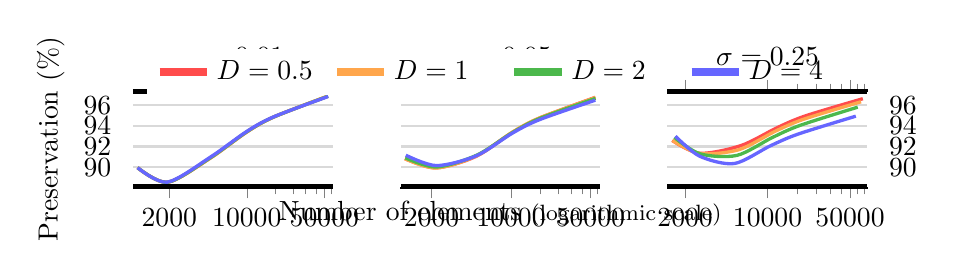
\begin{tikzpicture}
\begin{scope}[shift={(0.0\linewidth,0)}]
\begin{axis}[
 width=0.34\linewidth,height=0.23\linewidth,
 title=\normalsize\mbox{$\sigma=0.01$},
 xmode=log,enlarge x limits=0.025,
 ylabel=Preservation (\%),
 axis y line*=left,
 ymin=88.1171833333,ymax=97.3373908333,
 tick align=outside,
 x axis line style = ultra thick,y axis line style={white},
 xtick={2000,10000,50000},xticklabels={2000,10000,50000},
 minor xtick={18000,26000,34000,42000,58000,66000}, every y tick/.style={white},ymajorgrids,grid style={gray!30,thick}]
\addplot[very thick,mark=none,smooth,color=red!70] table[] {
	1036.16033333 89.9523333333
	1926.05033333 88.5353333333
	4681.20233333 90.8853333333
	9930.996 93.399
	17403.444 94.8616666667
	53726.3493333 96.885
};
\addplot[very thick,mark=none,smooth,color=orange!70] table[] {
	1036.16033333 89.9523333333
	1926.05033333 88.5353333333
	4680.99133333 90.8813333333
	9936.874 93.3996666667
	17410.171 94.863
	53781.8253333 96.8983333333
};
\addplot[very thick,mark=none,smooth,color=green!60!black!70] table[] {
	1036.16033333 89.9523333333
	1926.50133333 88.536
	4686.797 90.912
	9985.02666667 93.4346666667
	17498.657 94.8743333333
	54022.9776667 96.884
};
\addplot[very thick,mark=none,smooth,color=blue!60!] table[] {
	1036.16033333 89.9523333333
	1917.234 88.5486666667
	4693.193 90.976
	9995.812 93.474
	17515.7216667 94.892
	54124.1396667 96.8606666667
};
!\end{axis}
\end{scope}
\begin{scope}[shift={(0.28\linewidth,0)}]
\begin{axis}[
 width=0.34\linewidth,height=0.23\linewidth,
 title=\normalsize\mbox{$\sigma=0.05$},
 xmode=log,enlarge x limits=0.025,
 xlabel=Number of elements \footnotesize(logarithmic scale),x label style={at={(axis description cs:0.5,-0.05)},anchor=north},
 yticklabels={},
 legend style={at={(0.55,1.45)},legend style={text width=4em},legend style={draw=none},anchor=north,legend columns=-1},
 axis y line*=left,
 ymin=88.1171833333,ymax=97.3373908333,
 tick align=outside,
 x axis line style = ultra thick,y axis line style={white},
 xtick={2000,10000,50000},xticklabels={2000,10000,50000},
 minor xtick={18000,26000,34000,42000,58000,66000}, every y tick/.style={white},ymajorgrids,grid style={gray!30,thick}]
\addlegendimage{line width=3pt,mark=none,red!70}
\addlegendentry{$D=0.5$}
\addlegendimage{line width=3pt,mark=none,orange!70}
\addlegendentry{$D=1$}
\addlegendimage{line width=3pt,mark=none,green!60!black!70}
\addlegendentry{$D=2$}
\addlegendimage{line width=3pt,mark=none,blue!60!}
\addlegendentry{$D=4$}
\addplot[very thick,mark=none,smooth,color=red!70] table[] {
	1163.49166667 90.8273333333
	2177.14966667 89.939
	4885.092 91.0303333333
	10297.0083333 93.3843333333
	17952.9826667 94.7843333333
	55333.2983333 96.7773333333
};
\addplot[very thick,mark=none,smooth,color=orange!70] table[] {
	1163.74866667 90.8273333333
	2177.909 89.9183333333
	4930.84733333 91.0886666667
	10320.457 93.416
	18010.387 94.7963333333
	55424.09 96.7586666667
};
\addplot[very thick,mark=none,smooth,color=green!60!black!70] table[] {
	1172.79533333 90.9116666667
	2194.68166667 90.0166666667
	5002.62133333 91.1726666667
	10387.2886667 93.3883333333
	18071.808 94.7496666667
	55454.5933333 96.676
};
\addplot[very thick,mark=none,smooth,color=blue!60!] table[] {
	1184.77533333 91.1646666667
	2197.44466667 90.158
	4945.073 91.1046666667
	10276.6613333 93.305
	17925.9466667 94.6233333333
	55178.0426667 96.4986666667
};
!\end{axis}
\end{scope}
\begin{scope}[shift={(0.56\linewidth,0)}]
\begin{axis}[
 width=0.34\linewidth,height=0.23\linewidth,
 title=\normalsize\mbox{$\sigma=0.25$},
 xmode=log,enlarge x limits=0.025,
 axis y line*=right,
 ymin=88.1171833333,ymax=97.3373908333,
 tick align=outside,
 x axis line style = ultra thick,y axis line style={white},
 xtick={2000,10000,50000},xticklabels={2000,10000,50000},
 minor xtick={18000,26000,34000,42000,58000,66000}, every y tick/.style={white},ymajorgrids,grid style={gray!30,thick}]
\addplot[very thick,mark=none,smooth,color=red!70] table[] {
	1556.41833333 92.5956666667
	2657.71066667 91.3543333333
	5945.90766667 92.0966666667
	12147.856 93.8533333333
	21002.088 94.9846666667
	64168.1893333 96.6466666667
};
\addplot[very thick,mark=none,smooth,color=orange!70] table[] {
	1564.24866667 92.594
	2666.779 91.3296666667
	5704.51666667 91.6983333333
	11594.5613333 93.4843333333
	20113.86 94.6456666667
	61973.142 96.349
};
\addplot[very thick,mark=none,smooth,color=green!60!black!70] table[] {
	1623.46766667 92.8856666667
	2673.40233333 91.2983333333
	5489.90866667 91.1463333333
	11039.2793333 92.896
	19017.0963333 94.0743333333
	58137.1513333 95.827
};
\addplot[very thick,mark=none,smooth,color=blue!60!] table[] {
	1656.86533333 93.0056666667
	2657.24066667 91.0693333333
	5226.841 90.358
	10537.8956667 92.072
	18229.81 93.2213333333
	55998.5563333 94.9526666667
};
!\end{axis}
\end{scope}
\end{tikzpicture}
\end{center}
\caption{Element preservation results using mesh remodelling - Gottingen 459 airfoil}\centering\sffamily\footnotesize
Average of thirty optimisation scenarios\end{figure}

\begin{figure}[!h]
\begin{center}
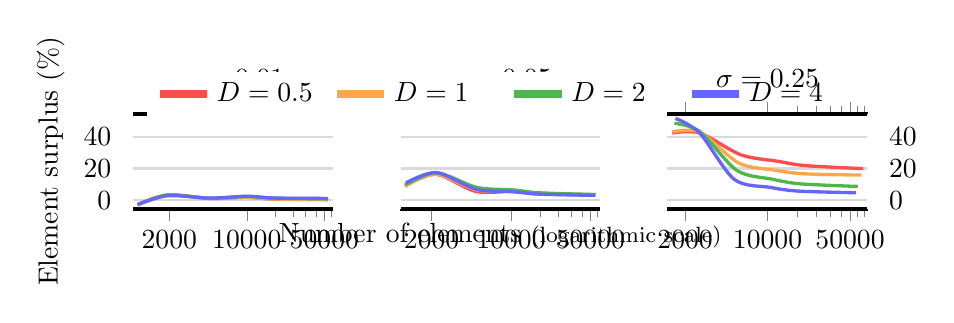
\begin{tikzpicture}
\begin{scope}[shift={(0.0\linewidth,0)}]
\begin{axis}[
 width=0.34\linewidth,height=0.23\linewidth,
 title=\normalsize\mbox{$\sigma=0.01$},
 xmode=log,enlarge x limits=0.025,
 ylabel=Element surplus (\%),
 axis y line*=left,
 ymin=-5.59784247357,ymax=54.4202499872,
 tick align=outside,
 x axis line style = ultra thick,y axis line style={white},
 xtick={2000,10000,50000},xticklabels={2000,10000,50000},
 minor xtick={18000,26000,34000,42000,58000,66000}, every y tick/.style={white},ymajorgrids,grid style={gray!30,thick}]
\addplot[very thick,mark=none,smooth,color=red!70] table[] {
	1036.16033333 -2.87593351843
	1926.05033333 3.21204716406
	4681.20233333 1.01837630643
	9930.996 1.76670319744
	17403.444 0.662798908144
	53726.3493333 0.310376501956
};
\addplot[very thick,mark=none,smooth,color=orange!70] table[] {
	1036.16033333 -2.87593351843
	1926.05033333 3.21204716406
	4680.99133333 1.01382301523
	9936.874 1.82693730502
	17410.171 0.701708370447
	53781.8253333 0.413953583144
};
\addplot[very thick,mark=none,smooth,color=green!60!black!70] table[] {
	1036.16033333 -2.87593351843
	1926.50133333 3.23621508557
	4686.797 1.13910685862
	9985.02666667 2.32037604337
	17498.657 1.21351789643
	54022.9776667 0.864199722164
};
\addplot[very thick,mark=none,smooth,color=blue!60!] table[] {
	1036.16033333 -2.87593351843
	1917.234 2.73960270295
	4693.193 1.27712984692
	9995.812 2.43089746702
	17515.7216667 1.31222118235
	54124.1396667 1.05307535644
};
!\end{axis}
\end{scope}
\begin{scope}[shift={(0.28\linewidth,0)}]
\begin{axis}[
 width=0.34\linewidth,height=0.23\linewidth,
 title=\normalsize\mbox{$\sigma=0.05$},
 xmode=log,enlarge x limits=0.025,
 xlabel=Number of elements \footnotesize(logarithmic scale),x label style={at={(axis description cs:0.5,-0.05)},anchor=north},
 yticklabels={},
 legend style={at={(0.55,1.45)},legend style={text width=4em},legend style={draw=none},anchor=north,legend columns=-1},
 axis y line*=left,
 ymin=-5.59784247357,ymax=54.4202499872,
 tick align=outside,
 x axis line style = ultra thick,y axis line style={white},
 xtick={2000,10000,50000},xticklabels={2000,10000,50000},
 minor xtick={18000,26000,34000,42000,58000,66000}, every y tick/.style={white},ymajorgrids,grid style={gray!30,thick}]
\addlegendimage{line width=3pt,mark=none,red!70}
\addlegendentry{$D=0.5$}
\addlegendimage{line width=3pt,mark=none,orange!70}
\addlegendentry{$D=1$}
\addlegendimage{line width=3pt,mark=none,green!60!black!70}
\addlegendentry{$D=2$}
\addlegendimage{line width=3pt,mark=none,blue!60!}
\addlegendentry{$D=4$}
\addplot[very thick,mark=none,smooth,color=red!70] table[] {
	1163.49166667 8.82242721425
	2177.14966667 16.3361322026
	4885.092 5.46439188348
	10297.0083333 5.51095957445
	17952.9826667 3.89163763232
	55333.2983333 3.28924690375
};
\addplot[very thick,mark=none,smooth,color=orange!70] table[] {
	1163.74866667 8.84646465654
	2177.909 16.376707228
	4930.84733333 6.45220509261
	10320.457 5.75123240328
	18010.387 4.22382924125
	55424.09 3.45872537616
};
\addplot[very thick,mark=none,smooth,color=green!60!black!70] table[] {
	1172.79533333 9.69260756677
	2194.68166667 17.2729557481
	5002.62133333 8.00173604577
	10387.2886667 6.43604036417
	18071.808 4.57926479162
	55454.5933333 3.5156651651
};
\addplot[very thick,mark=none,smooth,color=blue!60!] table[] {
	1184.77533333 10.813107795
	2197.44466667 17.4205968305
	4945.073 6.75932341999
	10276.6613333 5.30246877548
	17925.9466667 3.73518372339
	55178.0426667 2.99943513813
};
!\end{axis}
\end{scope}
\begin{scope}[shift={(0.56\linewidth,0)}]
\begin{axis}[
 width=0.34\linewidth,height=0.23\linewidth,
 title=\normalsize\mbox{$\sigma=0.25$},
 xmode=log,enlarge x limits=0.025,
 axis y line*=right,
 ymin=-5.59784247357,ymax=54.4202499872,
 tick align=outside,
 x axis line style = ultra thick,y axis line style={white},
 xtick={2000,10000,50000},xticklabels={2000,10000,50000},
 minor xtick={18000,26000,34000,42000,58000,66000}, every y tick/.style={white},ymajorgrids,grid style={gray!30,thick}]
\addplot[very thick,mark=none,smooth,color=red!70] table[] {
	1556.41833333 42.3738266006
	2657.71066667 42.3641376158
	5945.90766667 28.5837788446
	12147.856 24.5255422874
	21002.088 21.7544745104
	64168.1893333 19.8888272685
};
\addplot[very thick,mark=none,smooth,color=orange!70] table[] {
	1564.24866667 43.0901086544
	2666.779 42.8498960811
	5704.51666667 23.3635553397
	11594.5613333 18.8538156542
	20113.86 16.6051896685
	61973.142 15.7877040589
};
\addplot[very thick,mark=none,smooth,color=green!60!black!70] table[] {
	1623.46766667 48.5071841648
	2673.40233333 43.204684565
	5489.90866667 18.7225300906
	11039.2793333 13.1617172154
	19017.0963333 10.2469702431
	58137.1513333 8.62071949513
};
\addplot[very thick,mark=none,smooth,color=blue!60!] table[] {
	1656.86533333 51.5622455843
	2657.24066667 42.3389613822
	5226.841 13.0335358162
	10537.8956667 8.02212114302
	18229.81 5.68287005434
	55998.5563333 4.62506917032
};
!\end{axis}
\end{scope}
\end{tikzpicture}
\end{center}
\caption{Element surplus results on meshes from mesh remodelling - Gottingen 459 airfoil}\centering\sffamily\footnotesize
Average of thirty optimisation scenarios\end{figure}

\begin{figure}[!h]
\begin{center}
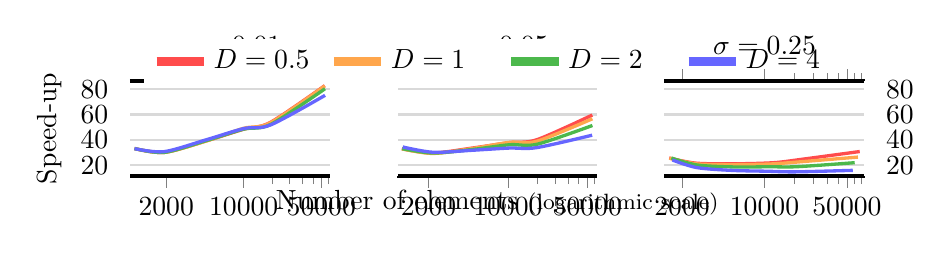
\begin{tikzpicture}
\begin{scope}[shift={(0.0\linewidth,0)}]
\begin{axis}[
 width=0.34\linewidth,height=0.23\linewidth,
 title=\normalsize\mbox{$\sigma=0.01$},
 xmode=log,enlarge x limits=0.025,
 ylabel=Speed-up,
 axis y line*=left,
 ymin=11.306562195,ymax=86.3569465468,
 tick align=outside,
 x axis line style = ultra thick,y axis line style={white},
 xtick={2000,10000,50000},xticklabels={2000,10000,50000},
 minor xtick={18000,26000,34000,42000,58000,66000}, every y tick/.style={white},ymajorgrids,grid style={gray!30,thick}]
\addplot[very thick,mark=none,smooth,color=red!70] table[] {
	1036.16033333 33.1281540505
	1926.05033333 30.0858381503
	4681.20233333 39.365481542
	9930.996 48.3273577553
	17403.444 53.7921724053
	53726.3493333 82.7831187206
};
\addplot[very thick,mark=none,smooth,color=orange!70] table[] {
	1036.16033333 33.1061712011
	1926.05033333 30.0771453337
	4680.99133333 39.3012375901
	9936.874 49.069325736
	17410.171 53.4374231015
	53781.8253333 82.5259502598
};
\addplot[very thick,mark=none,smooth,color=green!60!black!70] table[] {
	1036.16033333 33.1281540505
	1926.50133333 30.0858381503
	4686.797 39.591998904
	9985.02666667 48.4330573348
	17498.657 52.1465277111
	54022.9776667 80.3274190185
};
\addplot[very thick,mark=none,smooth,color=blue!60!] table[] {
	1036.16033333 33.0622929092
	1917.234 30.6618556701
	4693.193 40.2874668897
	9995.812 48.8913420596
	17515.7216667 51.7982539834
	54124.1396667 75.1285797874
};
!\end{axis}
\end{scope}
\begin{scope}[shift={(0.28\linewidth,0)}]
\begin{axis}[
 width=0.34\linewidth,height=0.23\linewidth,
 title=\normalsize\mbox{$\sigma=0.05$},
 xmode=log,enlarge x limits=0.025,
 xlabel=Number of elements \footnotesize(logarithmic scale),x label style={at={(axis description cs:0.5,-0.05)},anchor=north},
 yticklabels={},
 legend style={at={(0.55,1.45)},legend style={text width=4em},legend style={draw=none},anchor=north,legend columns=-1},
 axis y line*=left,
 ymin=11.306562195,ymax=86.3569465468,
 tick align=outside,
 x axis line style = ultra thick,y axis line style={white},
 xtick={2000,10000,50000},xticklabels={2000,10000,50000},
 minor xtick={18000,26000,34000,42000,58000,66000}, every y tick/.style={white},ymajorgrids,grid style={gray!30,thick}]
\addlegendimage{line width=3pt,mark=none,red!70}
\addlegendentry{$D=0.5$}
\addlegendimage{line width=3pt,mark=none,orange!70}
\addlegendentry{$D=1$}
\addlegendimage{line width=3pt,mark=none,green!60!black!70}
\addlegendentry{$D=2$}
\addlegendimage{line width=3pt,mark=none,blue!60!}
\addlegendentry{$D=4$}
\addplot[very thick,mark=none,smooth,color=red!70] table[] {
	1163.49166667 32.9511873351
	2177.14966667 29.5927293383
	4885.092 33.5371900826
	10297.0083333 37.7851198915
	17952.9826667 40.059654573
	55333.2983333 59.584514947
};
\addplot[very thick,mark=none,smooth,color=orange!70] table[] {
	1163.74866667 32.8861092824
	2177.909 29.2356902357
	4930.84733333 33.2086214846
	10320.457 38.0124023316
	18010.387 38.939245785
	55424.09 56.6006520167
};
\addplot[very thick,mark=none,smooth,color=green!60!black!70] table[] {
	1172.79533333 33.0165234633
	2194.68166667 29.5675368899
	5002.62133333 32.5042870036
	10387.2886667 36.1474230452
	18071.808 36.5270452553
	55454.5933333 51.3095314809
};
\addplot[very thick,mark=none,smooth,color=blue!60!] table[] {
	1184.77533333 34.356258597
	2197.44466667 30.1667631731
	4945.073 31.7870697264
	10276.6613333 33.4838040094
	17925.9466667 33.8364675747
	55178.0426667 43.6504442344
};
!\end{axis}
\end{scope}
\begin{scope}[shift={(0.56\linewidth,0)}]
\begin{axis}[
 width=0.34\linewidth,height=0.23\linewidth,
 title=\normalsize\mbox{$\sigma=0.25$},
 xmode=log,enlarge x limits=0.025,
 axis y line*=right,
 ymin=11.306562195,ymax=86.3569465468,
 tick align=outside,
 x axis line style = ultra thick,y axis line style={white},
 xtick={2000,10000,50000},xticklabels={2000,10000,50000},
 minor xtick={18000,26000,34000,42000,58000,66000}, every y tick/.style={white},ymajorgrids,grid style={gray!30,thick}]
\addplot[very thick,mark=none,smooth,color=red!70] table[] {
	1556.41833333 25.6236068896
	2657.71066667 21.5349080268
	5945.90766667 21.0973834959
	12147.856 21.9918791743
	21002.088 24.6988434885
	64168.1893333 30.7508832614
};
\addplot[very thick,mark=none,smooth,color=orange!70] table[] {
	1564.24866667 25.533064109
	2666.779 21.0165238678
	5704.51666667 20.382619101
	11594.5613333 20.9936605687
	20113.86 22.6470800748
	61973.142 26.3740512649
};
\addplot[very thick,mark=none,smooth,color=green!60!black!70] table[] {
	1623.46766667 25.6236068896
	2673.40233333 20.1374120407
	5489.90866667 18.5853791598
	11039.2793333 18.7277427694
	19017.0963333 18.7887833001
	58137.1513333 21.9512838373
};
\addplot[very thick,mark=none,smooth,color=blue!60!] table[] {
	1656.86533333 24.0632730733
	2657.24066667 18.0964342175
	5226.841 15.8718770019
	10537.8956667 15.1944102147
	18229.81 14.7102077438
	55998.5563333 15.8957546284
};
!\end{axis}
\end{scope}
\end{tikzpicture}
\end{center}
\caption{Speed-up results by mesh remodelling - Gottingen 459 airfoil}\centering\sffamily\footnotesize
Average of thirty optimisation scenarios\end{figure}

\pagebreak
\subsubsection{NACA 2412}
\vspace*{\fill} \begin{table}[!hp]
\begin{center}
\begin{tabular}{c|cc?c|c?c?c|c|c||c|c}
\multirow{2}{*}{\textbf{\large $\boldsymbol{\sigma}$}} & \multirow{2}{*}{\textbf{\large $\boldsymbol{I}$}} & \multirow{2}{*}{\textbf{\large $\boldsymbol{G}$}} & \multicolumn{2}{c?}{\textbf{\large Generation}} & \multirow{2}{*}{\textbf{\large $\boldsymbol{D}$}} & \multicolumn{5}{c}{\textbf{{\large Remodelling} }} \\\cline{4-5}\cline{7-11}
 & & & \textbf{\# Tri.} & \textbf{Time} & &\textbf{\# Tri.} & \textbf{Time} & \textbf{Preserv.} & \textbf{+ Tri.} & \textbf{Sp.-up} \\\toprule
\multirow{24}[13]{*}{.01} & \multirow{4}{*}{50} & \multirow{4}{*}{1} & \multirow{4}{*}{1048} & \multirow{4}{*}{1.64 ms} & .5 & 1115 & 0.05 ms & 90.49 \% & 6.45 \% & 32.23 \\\cline{6-11}
 & & & &  & 1 & 1115 & 0.05 ms & 90.49 \% & 6.45 \% & 32.23 \\\cline{6-11}
 & & & &  & 2 & 1115 & 0.05 ms & 90.52 \% & 6.43 \% & 32.31 \\\cline{6-11}
 & & & &  & 4 & 1114 & 0.05 ms & 90.58 \% & 6.37 \% & 33.25 \\\cmidrule[1.5pt]{2-11}
 & \multirow{4}{*}{100} & \multirow{4}{*}{2} & \multirow{4}{*}{1823} & \multirow{4}{*}{3.39 ms} & .5 & 2154 & 0.12 ms & 89.75 \% & 18.16 \% & 28.42 \\\cline{6-11}
 & & & &  & 1 & 2153 & 0.12 ms & 89.77 \% & 18.14 \% & 28.68 \\\cline{6-11}
 & & & &  & 2 & 2147 & 0.12 ms & 89.76 \% & 17.80 \% & 28.75 \\\cline{6-11}
 & & & &  & 4 & 2130 & 0.11 ms & 89.87 \% & 16.86 \% & 29.74 \\\cmidrule[1.5pt]{2-11}
 & \multirow{4}{*}{200} & \multirow{4}{*}{4} & \multirow{4}{*}{4618} & \multirow{4}{*}{9.49 ms} & .5 & 4981 & 0.29 ms & 91.19 \% & 7.86 \% & 32.36 \\\cline{6-11}
 & & & &  & 1 & 4967 & 0.29 ms & 91.17 \% & 7.54 \% & 32.64 \\\cline{6-11}
 & & & &  & 2 & 4982 & 0.30 ms & 91.18 \% & 7.88 \% & 32.02 \\\cline{6-11}
 & & & &  & 4 & 4907 & 0.29 ms & 91.12 \% & 6.26 \% & 32.18 \\\cmidrule[1.5pt]{2-11}
 & \multirow{4}{*}{300} & \multirow{4}{*}{6} & \multirow{4}{*}{9781} & \multirow{4}{*}{20.52 ms} & .5 & 10377 & 0.55 ms & 93.47 \% & 6.08 \% & 37.12 \\\cline{6-11}
 & & & &  & 1 & 10369 & 0.56 ms & 93.48 \% & 6.01 \% & 36.85 \\\cline{6-11}
 & & & &  & 2 & 10390 & 0.58 ms & 93.46 \% & 6.23 \% & 35.13 \\\cline{6-11}
 & & & &  & 4 & 10286 & 0.59 ms & 93.37 \% & 5.16 \% & 34.81 \\\cmidrule[1.5pt]{2-11}
 & \multirow{4}{*}{400} & \multirow{4}{*}{8} & \multirow{4}{*}{17288} & \multirow{4}{*}{35.91 ms} & .5 & 18148 & 0.96 ms & 94.86 \% & 4.97 \% & 37.22 \\\cline{6-11}
 & & & &  & 1 & 18134 & 0.98 ms & 94.86 \% & 4.89 \% & 36.78 \\\cline{6-11}
 & & & &  & 2 & 18107 & 1.02 ms & 94.80 \% & 4.74 \% & 35.30 \\\cline{6-11}
 & & & &  & 4 & 17957 & 1.07 ms & 94.68 \% & 3.87 \% & 33.61 \\\cmidrule[1.5pt]{2-11}
 & \multirow{4}{*}{700} & \multirow{4}{*}{14} & \multirow{4}{*}{53632} & \multirow{4}{*}{153.47 ms} & .5 & 55929 & 2.85 ms & 96.84 \% & 4.28 \% & 53.91 \\\cline{6-11}
 & & & &  & 1 & 55791 & 2.97 ms & 96.81 \% & 4.03 \% & 51.60 \\\cline{6-11}
 & & & &  & 2 & 55631 & 3.26 ms & 96.71 \% & 3.73 \% & 47.03 \\\cline{6-11}
 & & & &  & 4 & 55294 & 3.75 ms & 96.53 \% & 3.10 \% & 40.91\\\bottomrule
\end{tabular}\end{center}
\caption{Full results of mesh remodelling for $\sigma=0.01$ - NACA 2412 airfoil}\centering\sffamily\footnotesize
Average of thirty optimisation scenarios\end{table}
 \vspace*{\fill}
\begin{table}[!hp]
\begin{center}
\begin{tabular}{c|cc?c|c?c?c|c|c||c|c}
\multirow{2}{*}{\textbf{\large $\boldsymbol{\sigma}$}} & \multirow{2}{*}{\textbf{\large $\boldsymbol{I}$}} & \multirow{2}{*}{\textbf{\large $\boldsymbol{G}$}} & \multicolumn{2}{c?}{\textbf{\large Generation}} & \multirow{2}{*}{\textbf{\large $\boldsymbol{D}$}} & \multicolumn{5}{c}{\textbf{{\large Remodelling} }} \\\cline{4-5}\cline{7-11}
 & & & \textbf{\# Tri.} & \textbf{Time} & &\textbf{\# Tri.} & \textbf{Time} & \textbf{Preserv.} & \textbf{+ Tri.} & \textbf{Sp.-up} \\\toprule
\multirow{24}[13]{*}{.05} & \multirow{4}{*}{50} & \multirow{4}{*}{1} & \multirow{4}{*}{1062} & \multirow{4}{*}{1.65 ms} & .5 & 1295 & 0.05 ms & 91.44 \% & 21.95 \% & 31.17 \\\cline{6-11}
 & & & &  & 1 & 1303 & 0.05 ms & 91.48 \% & 22.73 \% & 31.25 \\\cline{6-11}
 & & & &  & 2 & 1298 & 0.05 ms & 91.52 \% & 22.18 \% & 31.21 \\\cline{6-11}
 & & & &  & 4 & 1299 & 0.05 ms & 91.62 \% & 22.29 \% & 32.14 \\\cmidrule[1.5pt]{2-11}
 & \multirow{4}{*}{100} & \multirow{4}{*}{2} & \multirow{4}{*}{1818} & \multirow{4}{*}{3.37 ms} & .5 & 2320 & 0.13 ms & 90.38 \% & 27.60 \% & 25.82 \\\cline{6-11}
 & & & &  & 1 & 2326 & 0.13 ms & 90.42 \% & 27.94 \% & 25.94 \\\cline{6-11}
 & & & &  & 2 & 2346 & 0.13 ms & 90.51 \% & 29.07 \% & 25.98 \\\cline{6-11}
 & & & &  & 4 & 2311 & 0.13 ms & 90.49 \% & 27.14 \% & 26.42 \\\cmidrule[1.5pt]{2-11}
 & \multirow{4}{*}{200} & \multirow{4}{*}{4} & \multirow{4}{*}{4617} & \multirow{4}{*}{9.38 ms} & .5 & 5139 & 0.33 ms & 91.28 \% & 11.29 \% & 28.84 \\\cline{6-11}
 & & & &  & 1 & 5118 & 0.32 ms & 91.27 \% & 10.84 \% & 28.89 \\\cline{6-11}
 & & & &  & 2 & 5136 & 0.34 ms & 91.24 \% & 11.24 \% & 27.89 \\\cline{6-11}
 & & & &  & 4 & 5030 & 0.35 ms & 91.06 \% & 8.94 \% & 26.97 \\\cmidrule[1.5pt]{2-11}
 & \multirow{4}{*}{300} & \multirow{4}{*}{6} & \multirow{4}{*}{9783} & \multirow{4}{*}{19.84 ms} & .5 & 10653 & 0.63 ms & 93.48 \% & 8.89 \% & 31.27 \\\cline{6-11}
 & & & &  & 1 & 10642 & 0.64 ms & 93.46 \% & 8.78 \% & 30.86 \\\cline{6-11}
 & & & &  & 2 & 10592 & 0.70 ms & 93.36 \% & 8.27 \% & 28.38 \\\cline{6-11}
 & & & &  & 4 & 10376 & 0.73 ms & 93.12 \% & 6.07 \% & 27.23 \\\cmidrule[1.5pt]{2-11}
 & \multirow{4}{*}{400} & \multirow{4}{*}{8} & \multirow{4}{*}{17288} & \multirow{4}{*}{35.80 ms} & .5 & 18583 & 1.11 ms & 94.83 \% & 7.49 \% & 32.13 \\\cline{6-11}
 & & & &  & 1 & 18521 & 1.13 ms & 94.79 \% & 7.13 \% & 31.60 \\\cline{6-11}
 & & & &  & 2 & 18418 & 1.22 ms & 94.66 \% & 6.54 \% & 29.31 \\\cline{6-11}
 & & & &  & 4 & 18060 & 1.34 ms & 94.40 \% & 4.46 \% & 26.72 \\\cmidrule[1.5pt]{2-11}
 & \multirow{4}{*}{700} & \multirow{4}{*}{14} & \multirow{4}{*}{53646} & \multirow{4}{*}{153.45 ms} & .5 & 57211 & 3.39 ms & 96.75 \% & 6.65 \% & 45.32 \\\cline{6-11}
 & & & &  & 1 & 56982 & 3.59 ms & 96.69 \% & 6.22 \% & 42.78 \\\cline{6-11}
 & & & &  & 2 & 56504 & 4.08 ms & 96.54 \% & 5.33 \% & 37.61 \\\cline{6-11}
 & & & &  & 4 & 55566 & 4.90 ms & 96.23 \% & 3.58 \% & 31.33\\\bottomrule
\end{tabular}\end{center}
\caption{Full results of mesh remodelling for $\sigma=0.05$ - NACA 2412 airfoil}\centering\sffamily\footnotesize
Average of thirty optimisation scenarios\end{table}

\begin{table}[!hp]
\begin{center}
\begin{tabular}{c|cc?c|c?c?c|c|c||c|c}
\multirow{2}{*}{\textbf{\large $\boldsymbol{\sigma}$}} & \multirow{2}{*}{\textbf{\large $\boldsymbol{I}$}} & \multirow{2}{*}{\textbf{\large $\boldsymbol{G}$}} & \multicolumn{2}{c?}{\textbf{\large Generation}} & \multirow{2}{*}{\textbf{\large $\boldsymbol{D}$}} & \multicolumn{5}{c}{\textbf{{\large Remodelling} }} \\\cline{4-5}\cline{7-11}
 & & & \textbf{\# Tri.} & \textbf{Time} & &\textbf{\# Tri.} & \textbf{Time} & \textbf{Preserv.} & \textbf{+ Tri.} & \textbf{Sp.-up} \\\toprule
\multirow{24}[13]{*}{.25} & \multirow{4}{*}{50} & \multirow{4}{*}{1} & \multirow{4}{*}{1084} & \multirow{4}{*}{1.67 ms} & .5 & 1570 & 0.07 ms & 92.66 \% & 44.88 \% & 25.39 \\\cline{6-11}
 & & & &  & 1 & 1592 & 0.07 ms & 92.72 \% & 46.85 \% & 25.20 \\\cline{6-11}
 & & & &  & 2 & 1610 & 0.07 ms & 92.78 \% & 48.57 \% & 24.96 \\\cline{6-11}
 & & & &  & 4 & 1664 & 0.07 ms & 93.04 \% & 53.51 \% & 23.36 \\\cmidrule[1.5pt]{2-11}
 & \multirow{4}{*}{100} & \multirow{4}{*}{2} & \multirow{4}{*}{1822} & \multirow{4}{*}{3.34 ms} & .5 & 2669 & 0.16 ms & 91.37 \% & 46.44 \% & 20.34 \\\cline{6-11}
 & & & &  & 1 & 2668 & 0.17 ms & 91.29 \% & 46.42 \% & 19.96 \\\cline{6-11}
 & & & &  & 2 & 2668 & 0.17 ms & 91.25 \% & 46.39 \% & 19.17 \\\cline{6-11}
 & & & &  & 4 & 2645 & 0.19 ms & 90.99 \% & 45.11 \% & 17.19 \\\cmidrule[1.5pt]{2-11}
 & \multirow{4}{*}{200} & \multirow{4}{*}{4} & \multirow{4}{*}{4610} & \multirow{4}{*}{8.98 ms} & .5 & 5943 & 0.44 ms & 92.09 \% & 28.91 \% & 20.40 \\\cline{6-11}
 & & & &  & 1 & 5717 & 0.46 ms & 91.68 \% & 24.01 \% & 19.67 \\\cline{6-11}
 & & & &  & 2 & 5463 & 0.51 ms & 91.06 \% & 18.50 \% & 17.76 \\\cline{6-11}
 & & & &  & 4 & 5240 & 0.60 ms & 90.29 \% & 13.67 \% & 15.07 \\\cmidrule[1.5pt]{2-11}
 & \multirow{4}{*}{300} & \multirow{4}{*}{6} & \multirow{4}{*}{9778} & \multirow{4}{*}{19.19 ms} & .5 & 12118 & 0.91 ms & 93.84 \% & 23.94 \% & 21.20 \\\cline{6-11}
 & & & &  & 1 & 11591 & 0.95 ms & 93.45 \% & 18.55 \% & 20.17 \\\cline{6-11}
 & & & &  & 2 & 10997 & 1.08 ms & 92.86 \% & 12.47 \% & 17.79 \\\cline{6-11}
 & & & &  & 4 & 10558 & 1.33 ms & 91.99 \% & 7.99 \% & 14.46 \\\cmidrule[1.5pt]{2-11}
 & \multirow{4}{*}{400} & \multirow{4}{*}{8} & \multirow{4}{*}{17273} & \multirow{4}{*}{35.35 ms} & .5 & 20974 & 1.51 ms & 94.97 \% & 21.43 \% & 23.36 \\\cline{6-11}
 & & & &  & 1 & 20113 & 1.69 ms & 94.61 \% & 16.45 \% & 20.90 \\\cline{6-11}
 & & & &  & 2 & 18937 & 1.99 ms & 94.02 \% & 9.64 \% & 17.81 \\\cline{6-11}
 & & & &  & 4 & 18201 & 2.55 ms & 93.12 \% & 5.37 \% & 13.86 \\\cmidrule[1.5pt]{2-11}
 & \multirow{4}{*}{700} & \multirow{4}{*}{14} & \multirow{4}{*}{53607} & \multirow{4}{*}{151.91 ms} & .5 & 64172 & 5.29 ms & 96.62 \% & 19.71 \% & 28.70 \\\cline{6-11}
 & & & &  & 1 & 61833 & 6.15 ms & 96.32 \% & 15.34 \% & 24.69 \\\cline{6-11}
 & & & &  & 2 & 57864 & 7.40 ms & 95.76 \% & 7.94 \% & 20.54 \\\cline{6-11}
 & & & &  & 4 & 55940 & 10.16 ms & 94.86 \% & 4.35 \% & 14.95\\\bottomrule
\end{tabular}\end{center}
\caption{Full results of mesh remodelling for $\sigma=0.25$ - NACA 2412 airfoil}\centering\sffamily\footnotesize
Average of thirty optimisation scenarios\end{table}
 \newpage
\begin{figure}[!h]
\begin{center}
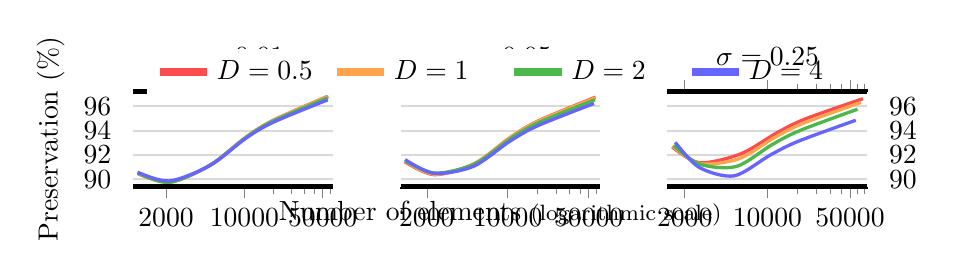
\begin{tikzpicture}
\begin{scope}[shift={(0.0\linewidth,0)}]
\begin{axis}[
 width=0.34\linewidth,height=0.23\linewidth,
 title=\normalsize\mbox{$\sigma=0.01$},
 xmode=log,enlarge x limits=0.025,
 ylabel=Preservation (\%),
 axis y line*=left,
 ymin=89.4003666667,ymax=97.2126816667,
 tick align=outside,
 x axis line style = ultra thick,y axis line style={white},
 xtick={2000,10000,50000},xticklabels={2000,10000,50000},
 minor xtick={18000,26000,34000,42000,58000,66000}, every y tick/.style={white},ymajorgrids,grid style={gray!30,thick}]
\addplot[very thick,mark=none,smooth,color=red!70] table[] {
	1115.258 90.4886666667
	2153.71966667 89.7546666667
	4981.13166667 91.187
	10376.6173333 93.4746666667
	18148.2636667 94.8566666667
	55929.1186667 96.8406666667
};
\addplot[very thick,mark=none,smooth,color=orange!70] table[] {
	1115.258 90.4886666667
	2153.35533333 89.765
	4966.71566667 91.173
	10369.0493333 93.477
	18133.7363333 94.8606666667
	55791.018 96.809
};
\addplot[very thick,mark=none,smooth,color=green!60!black!70] table[] {
	1115.04066667 90.516
	2147.23566667 89.7583333333
	4982.24466667 91.1813333333
	10390.4563333 93.456
	18107.314 94.7993333333
	55630.722 96.7063333333
};
\addplot[very thick,mark=none,smooth,color=blue!60!] table[] {
	1114.39433333 90.584
	2129.97033333 89.867
	4907.451 91.1223333333
	10285.6763333 93.369
	17956.7793333 94.6793333333
	55294.329 96.532
};
!\end{axis}
\end{scope}
\begin{scope}[shift={(0.28\linewidth,0)}]
\begin{axis}[
 width=0.34\linewidth,height=0.23\linewidth,
 title=\normalsize\mbox{$\sigma=0.05$},
 xmode=log,enlarge x limits=0.025,
 xlabel=Number of elements \footnotesize(logarithmic scale),x label style={at={(axis description cs:0.5,-0.05)},anchor=north},
 yticklabels={},
 legend style={at={(0.55,1.45)},legend style={text width=4em},legend style={draw=none},anchor=north,legend columns=-1},
 axis y line*=left,
 ymin=89.4003666667,ymax=97.2126816667,
 tick align=outside,
 x axis line style = ultra thick,y axis line style={white},
 xtick={2000,10000,50000},xticklabels={2000,10000,50000},
 minor xtick={18000,26000,34000,42000,58000,66000}, every y tick/.style={white},ymajorgrids,grid style={gray!30,thick}]
\addlegendimage{line width=3pt,mark=none,red!70}
\addlegendentry{$D=0.5$}
\addlegendimage{line width=3pt,mark=none,orange!70}
\addlegendentry{$D=1$}
\addlegendimage{line width=3pt,mark=none,green!60!black!70}
\addlegendentry{$D=2$}
\addlegendimage{line width=3pt,mark=none,blue!60!}
\addlegendentry{$D=4$}
\addplot[very thick,mark=none,smooth,color=red!70] table[] {
	1295.23666667 91.4383333333
	2319.814 90.383
	5138.91666667 91.278
	10652.52 93.4846666667
	18583.1506667 94.827
	57210.9673333 96.7516666667
};
\addplot[very thick,mark=none,smooth,color=orange!70] table[] {
	1303.43733333 91.4796666667
	2325.93266667 90.4166666667
	5118.09633333 91.2683333333
	10641.6626667 93.463
	18521.3283333 94.7893333333
	56982.0486667 96.688
};
\addplot[very thick,mark=none,smooth,color=green!60!black!70] table[] {
	1297.58333333 91.5216666667
	2346.43866667 90.5123333333
	5136.495 91.243
	10591.5073333 93.3576666667
	18417.8746667 94.661
	56504.481 96.5383333333
};
\addplot[very thick,mark=none,smooth,color=blue!60!] table[] {
	1298.755 91.6193333333
	2311.45166667 90.4946666667
	5030.275 91.057
	10376.187 93.117
	18059.9306667 94.3973333333
	55565.6503333 96.232
};
!\end{axis}
\end{scope}
\begin{scope}[shift={(0.56\linewidth,0)}]
\begin{axis}[
 width=0.34\linewidth,height=0.23\linewidth,
 title=\normalsize\mbox{$\sigma=0.25$},
 xmode=log,enlarge x limits=0.025,
 axis y line*=right,
 ymin=89.4003666667,ymax=97.2126816667,
 tick align=outside,
 x axis line style = ultra thick,y axis line style={white},
 xtick={2000,10000,50000},xticklabels={2000,10000,50000},
 minor xtick={18000,26000,34000,42000,58000,66000}, every y tick/.style={white},ymajorgrids,grid style={gray!30,thick}]
\addplot[very thick,mark=none,smooth,color=red!70] table[] {
	1570.24733333 92.6633333333
	2668.77166667 91.3656666667
	5942.79166667 92.089
	12118.3263333 93.8403333333
	20973.5136667 94.9653333333
	64172.085 96.6246666667
};
\addplot[very thick,mark=none,smooth,color=orange!70] table[] {
	1591.61966667 92.7176666667
	2668.32066667 91.2916666667
	5716.86733333 91.683
	11591.0006667 93.4543333333
	20113.2883333 94.611
	61832.7416667 96.32
};
\addplot[very thick,mark=none,smooth,color=green!60!black!70] table[] {
	1610.32533333 92.78
	2667.697 91.254
	5462.71833333 91.0553333333
	10996.7966667 92.86
	18937.3753333 94.0186666667
	57864.3813333 95.763
};
\addplot[very thick,mark=none,smooth,color=blue!60!] table[] {
	1663.819 93.043
	2644.519 90.9866666667
	5240.154 90.2863333333
	10558.453 91.991
	18200.8403333 93.1233333333
	55939.5143333 94.8556666667
};
!\end{axis}
\end{scope}
\end{tikzpicture}
\end{center}
\caption{Element preservation results using mesh remodelling - NACA 2412 airfoil}\centering\sffamily\footnotesize
Average of thirty optimisation scenarios\end{figure}

\begin{figure}[!h]
\begin{center}
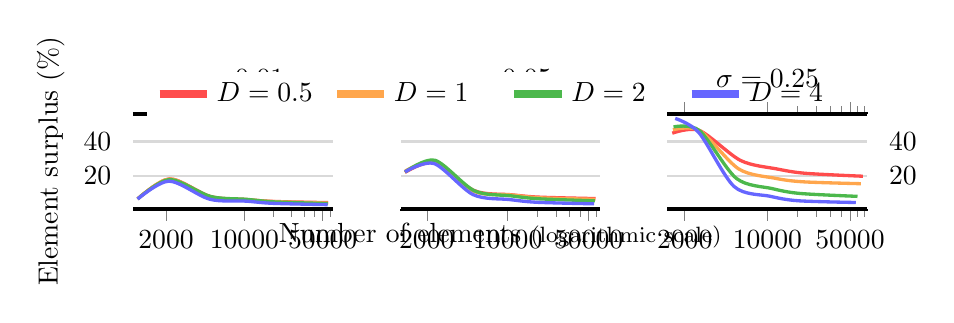
\begin{tikzpicture}
\begin{scope}[shift={(0.0\linewidth,0)}]
\begin{axis}[
 width=0.34\linewidth,height=0.23\linewidth,
 title=\normalsize\mbox{$\sigma=0.01$},
 xmode=log,enlarge x limits=0.025,
 ylabel=Element surplus (\%),
 axis y line*=left,
 ymin=0.579218231148,ymax=56.1570690355,
 tick align=outside,
 x axis line style = ultra thick,y axis line style={white},
 xtick={2000,10000,50000},xticklabels={2000,10000,50000},
 minor xtick={18000,26000,34000,42000,58000,66000}, every y tick/.style={white},ymajorgrids,grid style={gray!30,thick}]
\addplot[very thick,mark=none,smooth,color=red!70] table[] {
	1115.258 6.45076001623
	2153.71966667 18.1595471241
	4981.13166667 7.85570510779
	10376.6173333 6.08478719539
	18148.2636667 4.97346703252
	55929.1186667 4.2833609587
};
\addplot[very thick,mark=none,smooth,color=orange!70] table[] {
	1115.258 6.45076001623
	2153.35533333 18.1395587002
	4966.71566667 7.54355759817
	10369.0493333 6.0074161559
	18133.7363333 4.88943780665
	55791.018 4.02586357605
};
\addplot[very thick,mark=none,smooth,color=green!60!black!70] table[] {
	1115.04066667 6.43001566962
	2147.23566667 17.8038153567
	4982.24466667 7.8798047317
	10390.4563333 6.22626946489
	18107.314 4.73660533804
	55630.722 3.72698159781
};
\addplot[very thick,mark=none,smooth,color=blue!60!] table[] {
	1114.39433333 6.36832350999
	2129.97033333 16.8565871732
	4907.451 6.2603085618
	10285.6763333 5.15505679073
	17956.7793333 3.86588039384
	55294.329 3.09975568259
};
!\end{axis}
\end{scope}
\begin{scope}[shift={(0.28\linewidth,0)}]
\begin{axis}[
 width=0.34\linewidth,height=0.23\linewidth,
 title=\normalsize\mbox{$\sigma=0.05$},
 xmode=log,enlarge x limits=0.025,
 xlabel=Number of elements \footnotesize(logarithmic scale),x label style={at={(axis description cs:0.5,-0.05)},anchor=north},
 yticklabels={},
 legend style={at={(0.55,1.45)},legend style={text width=4em},legend style={draw=none},anchor=north,legend columns=-1},
 axis y line*=left,
 ymin=0.579218231148,ymax=56.1570690355,
 tick align=outside,
 x axis line style = ultra thick,y axis line style={white},
 xtick={2000,10000,50000},xticklabels={2000,10000,50000},
 minor xtick={18000,26000,34000,42000,58000,66000}, every y tick/.style={white},ymajorgrids,grid style={gray!30,thick}]
\addlegendimage{line width=3pt,mark=none,red!70}
\addlegendentry{$D=0.5$}
\addlegendimage{line width=3pt,mark=none,orange!70}
\addlegendentry{$D=1$}
\addlegendimage{line width=3pt,mark=none,green!60!black!70}
\addlegendentry{$D=2$}
\addlegendimage{line width=3pt,mark=none,blue!60!}
\addlegendentry{$D=4$}
\addplot[very thick,mark=none,smooth,color=red!70] table[] {
	1295.23666667 21.9546719093
	2319.814 27.6019219564
	5138.91666667 11.2929085986
	10652.52 8.89356238619
	18583.1506667 7.49118337079
	57210.9673333 6.64526523409
};
\addplot[very thick,mark=none,smooth,color=orange!70] table[] {
	1303.43733333 22.726816212
	2325.93266667 27.9384806746
	5118.09633333 10.8420051096
	10641.6626667 8.78257515456
	18521.3283333 7.13358223587
	56982.0486667 6.21854474567
};
\addplot[very thick,mark=none,smooth,color=green!60!black!70] table[] {
	1297.58333333 22.1756253233
	2346.43866667 29.0664180919
	5136.495 11.2404628509
	10591.5073333 8.26987084428
	18417.8746667 6.53517148984
	56504.481 5.32832504037
};
\addplot[very thick,mark=none,smooth,color=blue!60!] table[] {
	1298.755 22.2859451031
	2311.45166667 27.1419498184
	5030.275 8.9400689122
	10376.187 6.06879559159
	18059.9306667 4.46470320216
	55565.6503333 3.57827867473
};
!\end{axis}
\end{scope}
\begin{scope}[shift={(0.56\linewidth,0)}]
\begin{axis}[
 width=0.34\linewidth,height=0.23\linewidth,
 title=\normalsize\mbox{$\sigma=0.25$},
 xmode=log,enlarge x limits=0.025,
 axis y line*=right,
 ymin=0.579218231148,ymax=56.1570690355,
 tick align=outside,
 x axis line style = ultra thick,y axis line style={white},
 xtick={2000,10000,50000},xticklabels={2000,10000,50000},
 minor xtick={18000,26000,34000,42000,58000,66000}, every y tick/.style={white},ymajorgrids,grid style={gray!30,thick}]
\addplot[very thick,mark=none,smooth,color=red!70] table[] {
	1570.24733333 44.8772136043
	2668.77166667 46.4446499962
	5942.79166667 28.9147971233
	12118.3263333 23.9403241058
	20973.5136667 21.4256425054
	64172.085 19.7086445581
};
\addplot[very thick,mark=none,smooth,color=orange!70] table[] {
	1591.61966667 46.8491093915
	2668.32066667 46.4199020802
	5716.86733333 24.0139035314
	11591.0006667 18.5470946912
	20113.2883333 16.4453890553
	61832.7416667 15.3447592396
};
\addplot[very thick,mark=none,smooth,color=green!60!black!70] table[] {
	1610.32533333 48.5749679921
	2667.697 46.3856793522
	5462.71833333 18.5007426111
	10996.7966667 12.4698663414
	18937.3753333 9.63746960863
	57864.3813333 7.9420538947
};
\addplot[very thick,mark=none,smooth,color=blue!60!] table[] {
	1663.819 53.5105047115
	2644.519 45.1138230372
	5240.154 13.6727362653
	10558.453 7.98670137111
	18200.8403333 5.37331830694
	55939.5143333 4.35134588631
};
!\end{axis}
\end{scope}
\end{tikzpicture}
\end{center}
\caption{Element surplus results on meshes from mesh remodelling - NACA 2412 airfoil}\centering\sffamily\footnotesize
Average of thirty optimisation scenarios\end{figure}

\begin{figure}[!h]
\begin{center}
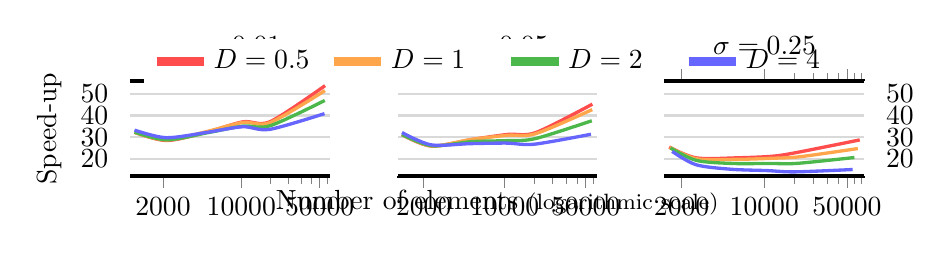
\begin{tikzpicture}
\begin{scope}[shift={(0.0\linewidth,0)}]
\begin{axis}[
 width=0.34\linewidth,height=0.23\linewidth,
 title=\normalsize\mbox{$\sigma=0.01$},
 xmode=log,enlarge x limits=0.025,
 ylabel=Speed-up,
 axis y line*=left,
 ymin=11.8624839129,ymax=56.0132621464,
 tick align=outside,
 x axis line style = ultra thick,y axis line style={white},
 xtick={2000,10000,50000},xticklabels={2000,10000,50000},
 minor xtick={18000,26000,34000,42000,58000,66000}, every y tick/.style={white},ymajorgrids,grid style={gray!30,thick}]
\addplot[very thick,mark=none,smooth,color=red!70] table[] {
	1115.258 32.2252783235
	2153.71966667 28.4233025985
	4981.13166667 32.3616513135
	10376.6173333 37.1198070546
	18148.2636667 37.2211013612
	55929.1186667 53.9108441353
};
\addplot[very thick,mark=none,smooth,color=orange!70] table[] {
	1115.258 32.2252783235
	2153.35533333 28.6797293487
	4966.71566667 32.6400550585
	10369.0493333 36.8487460346
	18133.7363333 36.781442032
	55791.018 51.602071238
};
\addplot[very thick,mark=none,smooth,color=green!60!black!70] table[] {
	1115.04066667 32.3099146422
	2147.23566667 28.7526851328
	4982.24466667 32.0229574612
	10390.4563333 35.1327968955
	18107.314 35.2980375455
	55630.722 47.0337528604
};
\addplot[very thick,mark=none,smooth,color=blue!60!] table[] {
	1114.39433333 33.2486486486
	2129.97033333 29.736042093
	4907.451 32.1786723962
	10285.6763333 34.8070334144
	17956.7793333 33.6131407357
	55294.329 40.9142532147
};
!\end{axis}
\end{scope}
\begin{scope}[shift={(0.28\linewidth,0)}]
\begin{axis}[
 width=0.34\linewidth,height=0.23\linewidth,
 title=\normalsize\mbox{$\sigma=0.05$},
 xmode=log,enlarge x limits=0.025,
 xlabel=Number of elements \footnotesize(logarithmic scale),x label style={at={(axis description cs:0.5,-0.05)},anchor=north},
 yticklabels={},
 legend style={at={(0.55,1.45)},legend style={text width=4em},legend style={draw=none},anchor=north,legend columns=-1},
 axis y line*=left,
 ymin=11.8624839129,ymax=56.0132621464,
 tick align=outside,
 x axis line style = ultra thick,y axis line style={white},
 xtick={2000,10000,50000},xticklabels={2000,10000,50000},
 minor xtick={18000,26000,34000,42000,58000,66000}, every y tick/.style={white},ymajorgrids,grid style={gray!30,thick}]
\addlegendimage{line width=3pt,mark=none,red!70}
\addlegendentry{$D=0.5$}
\addlegendimage{line width=3pt,mark=none,orange!70}
\addlegendentry{$D=1$}
\addlegendimage{line width=3pt,mark=none,green!60!black!70}
\addlegendentry{$D=2$}
\addlegendimage{line width=3pt,mark=none,blue!60!}
\addlegendentry{$D=4$}
\addplot[very thick,mark=none,smooth,color=red!70] table[] {
	1295.23666667 31.1677135678
	2319.814 25.819110884
	5138.91666667 28.8439934399
	10652.52 31.2666106413
	18583.1506667 32.1278454129
	57210.9673333 45.322070276
};
\addplot[very thick,mark=none,smooth,color=orange!70] table[] {
	1303.43733333 31.2462216625
	2325.93266667 25.9383983573
	5118.09633333 28.8854444673
	10641.6626667 30.8565726726
	18521.3283333 31.5976112026
	56982.0486667 42.7786265217
};
\addplot[very thick,mark=none,smooth,color=green!60!black!70] table[] {
	1297.58333333 31.206918239
	2346.43866667 25.9784061697
	5136.495 27.8947264076
	10591.5073333 28.3847510967
	18417.8746667 29.3148284615
	56504.481 37.6052412306
};
\addplot[very thick,mark=none,smooth,color=blue!60!] table[] {
	1298.755 32.1366580311
	2311.45166667 26.419869281
	5030.275 26.9671298515
	10376.187 27.2292105022
	18059.9306667 26.7213832566
	55565.6503333 31.3293406653
};
!\end{axis}
\end{scope}
\begin{scope}[shift={(0.56\linewidth,0)}]
\begin{axis}[
 width=0.34\linewidth,height=0.23\linewidth,
 title=\normalsize\mbox{$\sigma=0.25$},
 xmode=log,enlarge x limits=0.025,
 axis y line*=right,
 ymin=11.8624839129,ymax=56.0132621464,
 tick align=outside,
 x axis line style = ultra thick,y axis line style={white},
 xtick={2000,10000,50000},xticklabels={2000,10000,50000},
 minor xtick={18000,26000,34000,42000,58000,66000}, every y tick/.style={white},ymajorgrids,grid style={gray!30,thick}]
\addplot[very thick,mark=none,smooth,color=red!70] table[] {
	1570.24733333 25.3942307692
	2668.77166667 20.3444849959
	5942.79166667 20.3993484355
	12118.3263333 21.1972603749
	20973.5136667 23.3575518654
	64172.085 28.7048664038
};
\addplot[very thick,mark=none,smooth,color=orange!70] table[] {
	1591.61966667 25.202913109
	2668.32066667 19.9560461416
	5716.86733333 19.6677136596
	11591.0006667 20.1707838397
	20113.2883333 20.9037567014
	61832.7416667 24.6911307363
};
\addplot[very thick,mark=none,smooth,color=green!60!black!70] table[] {
	1610.32533333 24.9646766169
	2667.697 19.1742786165
	5462.71833333 17.7571061136
	10996.7966667 17.7863123745
	18937.3753333 17.8070988432
	57864.3813333 20.5389416945
};
\addplot[very thick,mark=none,smooth,color=blue!60!] table[] {
	1663.819 23.3608007449
	2644.519 17.1872216513
	5240.154 15.073955884
	10558.453 14.4611249278
	18200.8403333 13.8647867807
	55939.5143333 14.9547214638
};
!\end{axis}
\end{scope}
\end{tikzpicture}
\end{center}
\caption{Speed-up results by mesh remodelling - NACA 2412 airfoil}\centering\sffamily\footnotesize
Average of thirty optimisation scenarios\end{figure}

\pagebreak
\subsubsection{Clark-Y}
\vspace*{\fill} \begin{table}[!hp]
\begin{center}
\begin{tabular}{c|cc?c|c?c?c|c|c||c|c}
\multirow{2}{*}{\textbf{\large $\boldsymbol{\sigma}$}} & \multirow{2}{*}{\textbf{\large $\boldsymbol{I}$}} & \multirow{2}{*}{\textbf{\large $\boldsymbol{G}$}} & \multicolumn{2}{c?}{\textbf{\large Generation}} & \multirow{2}{*}{\textbf{\large $\boldsymbol{D}$}} & \multicolumn{5}{c}{\textbf{{\large Remodelling} }} \\\cline{4-5}\cline{7-11}
 & & & \textbf{\# Tri.} & \textbf{Time} & &\textbf{\# Tri.} & \textbf{Time} & \textbf{Preserv.} & \textbf{+ Tri.} & \textbf{Sp.-up} \\\toprule
\multirow{24}[11]{*}{.01} & \multirow{4}{*}{50} & \multirow{4}{*}{1} & \multirow{4}{*}{1052} & \multirow{4}{*}{1.68 ms} & .5 & 1269 & 0.05 ms & 91.31 \% & 20.65 \% & 31.69 \\\cline{6-11}
 & & & &  & 1 & 1264 & 0.05 ms & 91.27 \% & 20.14 \% & 31.61 \\\cline{6-11}
 & & & &  & 2 & 1268 & 0.05 ms & 91.35 \% & 20.56 \% & 31.97 \\\cline{6-11}
 & & & &  & 4 & 1271 & 0.05 ms & 91.50 \% & 20.87 \% & 32.95 \\\cmidrule[1.5pt]{2-11}
 & \multirow{4}{*}{100} & \multirow{4}{*}{2} & \multirow{4}{*}{1850} & \multirow{4}{*}{3.52 ms} & .5 & 2276 & 0.13 ms & 90.20 \% & 23.05 \% & 26.87 \\\cline{6-11}
 & & & &  & 1 & 2292 & 0.13 ms & 90.29 \% & 23.87 \% & 26.88 \\\cline{6-11}
 & & & &  & 2 & 2317 & 0.13 ms & 90.39 \% & 25.25 \% & 26.82 \\\cline{6-11}
 & & & &  & 4 & 2295 & 0.13 ms & 90.40 \% & 24.07 \% & 27.41 \\\cmidrule[1.5pt]{2-11}
 & \multirow{4}{*}{200} & \multirow{4}{*}{4} & \multirow{4}{*}{4627} & \multirow{4}{*}{9.81 ms} & .5 & 5182 & 0.34 ms & 91.36 \% & 12.00 \% & 29.25 \\\cline{6-11}
 & & & &  & 1 & 5161 & 0.33 ms & 91.33 \% & 11.54 \% & 29.44 \\\cline{6-11}
 & & & &  & 2 & 5159 & 0.35 ms & 91.24 \% & 11.50 \% & 28.17 \\\cline{6-11}
 & & & &  & 4 & 5047 & 0.36 ms & 91.05 \% & 9.08 \% & 27.11 \\\cmidrule[1.5pt]{2-11}
 & \multirow{4}{*}{300} & \multirow{4}{*}{6} & \multirow{4}{*}{9833} & \multirow{4}{*}{20.79 ms} & .5 & 10781 & 0.66 ms & 93.53 \% & 9.64 \% & 31.71 \\\cline{6-11}
 & & & &  & 1 & 10724 & 0.67 ms & 93.48 \% & 9.06 \% & 31.07 \\\cline{6-11}
 & & & &  & 2 & 10662 & 0.70 ms & 93.37 \% & 8.43 \% & 29.90 \\\cline{6-11}
 & & & &  & 4 & 10421 & 0.76 ms & 93.10 \% & 5.97 \% & 27.42 \\\cmidrule[1.5pt]{2-11}
 & \multirow{4}{*}{400} & \multirow{4}{*}{8} & \multirow{4}{*}{17337} & \multirow{4}{*}{37.37 ms} & .5 & 18828 & 1.13 ms & 94.86 \% & 8.60 \% & 32.94 \\\cline{6-11}
 & & & &  & 1 & 18701 & 1.16 ms & 94.80 \% & 7.86 \% & 32.28 \\\cline{6-11}
 & & & &  & 2 & 18531 & 1.26 ms & 94.66 \% & 6.88 \% & 29.72 \\\cline{6-11}
 & & & &  & 4 & 18138 & 1.38 ms & 94.37 \% & 4.62 \% & 27.00 \\\cmidrule[1.5pt]{2-11}
 & \multirow{4}{*}{700} & \multirow{4}{*}{14} & \multirow{4}{*}{53738} & \multirow{4}{*}{157.90 ms} & .5 & 57984 & 3.49 ms & 96.77 \% & 7.90 \% & 45.20 \\\cline{6-11}
 & & & &  & 1 & 57488 & 3.72 ms & 96.69 \% & 6.98 \% & 42.39 \\\cline{6-11}
 & & & &  & 2 & 56804 & 4.23 ms & 96.52 \% & 5.71 \% & 37.35 \\\cline{6-11}
 & & & &  & 4 & 55824 & 5.07 ms & 96.18 \% & 3.88 \% & 31.14\\\bottomrule
\end{tabular}\end{center}
\caption{Full results of mesh remodelling for $\sigma=0.01$ - Clark-Y airfoil}\centering\sffamily\footnotesize
Average of thirty optimisation scenarios\end{table}
 \vspace*{\fill}
\begin{table}[!hp]
\begin{center}
\begin{tabular}{c|cc?c|c?c?c|c|c||c|c}
\multirow{2}{*}{\textbf{\large $\boldsymbol{\sigma}$}} & \multirow{2}{*}{\textbf{\large $\boldsymbol{I}$}} & \multirow{2}{*}{\textbf{\large $\boldsymbol{G}$}} & \multicolumn{2}{c?}{\textbf{\large Generation}} & \multirow{2}{*}{\textbf{\large $\boldsymbol{D}$}} & \multicolumn{5}{c}{\textbf{{\large Remodelling} }} \\\cline{4-5}\cline{7-11}
 & & & \textbf{\# Tri.} & \textbf{Time} & &\textbf{\# Tri.} & \textbf{Time} & \textbf{Preserv.} & \textbf{+ Tri.} & \textbf{Sp.-up} \\\toprule
\multirow{24}[13]{*}{.05} & \multirow{4}{*}{50} & \multirow{4}{*}{1} & \multirow{4}{*}{1057} & \multirow{4}{*}{1.68 ms} & .5 & 1386 & 0.06 ms & 91.85 \% & 31.09 \% & 29.81 \\\cline{6-11}
 & & & &  & 1 & 1384 & 0.06 ms & 91.85 \% & 30.87 \% & 29.60 \\\cline{6-11}
 & & & &  & 2 & 1397 & 0.06 ms & 91.97 \% & 32.13 \% & 30.38 \\\cline{6-11}
 & & & &  & 4 & 1381 & 0.05 ms & 91.99 \% & 30.63 \% & 31.08 \\\cmidrule[1.5pt]{2-11}
 & \multirow{4}{*}{100} & \multirow{4}{*}{2} & \multirow{4}{*}{1844} & \multirow{4}{*}{3.49 ms} & .5 & 2377 & 0.14 ms & 90.54 \% & 28.93 \% & 25.43 \\\cline{6-11}
 & & & &  & 1 & 2384 & 0.13 ms & 90.59 \% & 29.33 \% & 26.00 \\\cline{6-11}
 & & & &  & 2 & 2420 & 0.14 ms & 90.75 \% & 31.26 \% & 25.39 \\\cline{6-11}
 & & & &  & 4 & 2398 & 0.14 ms & 90.74 \% & 30.05 \% & 25.37 \\\cmidrule[1.5pt]{2-11}
 & \multirow{4}{*}{200} & \multirow{4}{*}{4} & \multirow{4}{*}{4627} & \multirow{4}{*}{9.55 ms} & .5 & 5279 & 0.35 ms & 91.44 \% & 14.09 \% & 27.40 \\\cline{6-11}
 & & & &  & 1 & 5254 & 0.35 ms & 91.40 \% & 13.56 \% & 27.21 \\\cline{6-11}
 & & & &  & 2 & 5228 & 0.37 ms & 91.28 \% & 13.01 \% & 25.98 \\\cline{6-11}
 & & & &  & 4 & 5081 & 0.39 ms & 90.96 \% & 9.83 \% & 24.26 \\\cmidrule[1.5pt]{2-11}
 & \multirow{4}{*}{300} & \multirow{4}{*}{6} & \multirow{4}{*}{9834} & \multirow{4}{*}{20.30 ms} & .5 & 10966 & 0.69 ms & 93.56 \% & 11.51 \% & 29.28 \\\cline{6-11}
 & & & &  & 1 & 10885 & 0.71 ms & 93.49 \% & 10.69 \% & 28.75 \\\cline{6-11}
 & & & &  & 2 & 10717 & 0.75 ms & 93.29 \% & 8.98 \% & 27.12 \\\cline{6-11}
 & & & &  & 4 & 10439 & 0.83 ms & 92.94 \% & 6.16 \% & 24.37 \\\cmidrule[1.5pt]{2-11}
 & \multirow{4}{*}{400} & \multirow{4}{*}{8} & \multirow{4}{*}{17336} & \multirow{4}{*}{37.06 ms} & .5 & 19098 & 1.19 ms & 94.86 \% & 10.16 \% & 31.21 \\\cline{6-11}
 & & & &  & 1 & 18943 & 1.24 ms & 94.77 \% & 9.27 \% & 29.79 \\\cline{6-11}
 & & & &  & 2 & 18604 & 1.35 ms & 94.57 \% & 7.31 \% & 27.46 \\\cline{6-11}
 & & & &  & 4 & 18175 & 1.55 ms & 94.20 \% & 4.84 \% & 23.86 \\\cmidrule[1.5pt]{2-11}
 & \multirow{4}{*}{700} & \multirow{4}{*}{14} & \multirow{4}{*}{53740} & \multirow{4}{*}{157.14 ms} & .5 & 58814 & 3.72 ms & 96.74 \% & 9.44 \% & 42.21 \\\cline{6-11}
 & & & &  & 1 & 58424 & 4.09 ms & 96.63 \% & 8.72 \% & 38.46 \\\cline{6-11}
 & & & &  & 2 & 56995 & 4.65 ms & 96.41 \% & 6.06 \% & 33.81 \\\cline{6-11}
 & & & &  & 4 & 55852 & 5.81 ms & 96.00 \% & 3.93 \% & 27.05\\\bottomrule
\end{tabular}\end{center}
\caption{Full results of mesh remodelling for $\sigma=0.05$ - Clark-Y airfoil}\centering\sffamily\footnotesize
Average of thirty optimisation scenarios\end{table}

\begin{table}[!hp]
\begin{center}
\begin{tabular}{c|cc?c|c?c?c|c|c||c|c}
\multirow{2}{*}{\textbf{\large $\boldsymbol{\sigma}$}} & \multirow{2}{*}{\textbf{\large $\boldsymbol{I}$}} & \multirow{2}{*}{\textbf{\large $\boldsymbol{G}$}} & \multicolumn{2}{c?}{\textbf{\large Generation}} & \multirow{2}{*}{\textbf{\large $\boldsymbol{D}$}} & \multicolumn{5}{c}{\textbf{{\large Remodelling} }} \\\cline{4-5}\cline{7-11}
 & & & \textbf{\# Tri.} & \textbf{Time} & &\textbf{\# Tri.} & \textbf{Time} & \textbf{Preserv.} & \textbf{+ Tri.} & \textbf{Sp.-up} \\\toprule
\multirow{24}[11]{*}{.25} & \multirow{4}{*}{50} & \multirow{4}{*}{1} & \multirow{4}{*}{1061} & \multirow{4}{*}{1.67 ms} & .5 & 1568 & 0.07 ms & 92.55 \% & 47.84 \% & 24.36 \\\cline{6-11}
 & & & &  & 1 & 1588 & 0.07 ms & 92.64 \% & 49.75 \% & 24.67 \\\cline{6-11}
 & & & &  & 2 & 1607 & 0.07 ms & 92.77 \% & 51.58 \% & 24.35 \\\cline{6-11}
 & & & &  & 4 & 1694 & 0.07 ms & 93.12 \% & 59.69 \% & 22.85 \\\cmidrule[1.5pt]{2-11}
 & \multirow{4}{*}{100} & \multirow{4}{*}{2} & \multirow{4}{*}{1860} & \multirow{4}{*}{3.48 ms} & .5 & 2702 & 0.17 ms & 91.46 \% & 45.28 \% & 20.74 \\\cline{6-11}
 & & & &  & 1 & 2687 & 0.17 ms & 91.38 \% & 44.47 \% & 20.69 \\\cline{6-11}
 & & & &  & 2 & 2684 & 0.18 ms & 91.29 \% & 44.30 \% & 19.69 \\\cline{6-11}
 & & & &  & 4 & 2676 & 0.20 ms & 91.04 \% & 43.88 \% & 17.37 \\\cmidrule[1.5pt]{2-11}
 & \multirow{4}{*}{200} & \multirow{4}{*}{4} & \multirow{4}{*}{4617} & \multirow{4}{*}{9.28 ms} & .5 & 6014 & 0.45 ms & 92.14 \% & 30.27 \% & 20.67 \\\cline{6-11}
 & & & &  & 1 & 5772 & 0.47 ms & 91.72 \% & 25.01 \% & 19.70 \\\cline{6-11}
 & & & &  & 2 & 5507 & 0.52 ms & 91.09 \% & 19.28 \% & 17.84 \\\cline{6-11}
 & & & &  & 4 & 5274 & 0.61 ms & 90.27 \% & 14.24 \% & 15.23 \\\cmidrule[1.5pt]{2-11}
 & \multirow{4}{*}{300} & \multirow{4}{*}{6} & \multirow{4}{*}{9822} & \multirow{4}{*}{19.84 ms} & .5 & 12278 & 0.92 ms & 93.88 \% & 25.00 \% & 21.51 \\\cline{6-11}
 & & & &  & 1 & 11711 & 0.99 ms & 93.47 \% & 19.23 \% & 20.11 \\\cline{6-11}
 & & & &  & 2 & 11073 & 1.11 ms & 92.82 \% & 12.73 \% & 17.82 \\\cline{6-11}
 & & & &  & 4 & 10604 & 1.37 ms & 91.95 \% & 7.96 \% & 14.47 \\\cmidrule[1.5pt]{2-11}
 & \multirow{4}{*}{400} & \multirow{4}{*}{8} & \multirow{4}{*}{17313} & \multirow{4}{*}{36.42 ms} & .5 & 21270 & 1.54 ms & 95.00 \% & 22.86 \% & 23.60 \\\cline{6-11}
 & & & &  & 1 & 20286 & 1.70 ms & 94.63 \% & 17.17 \% & 21.43 \\\cline{6-11}
 & & & &  & 2 & 19096 & 2.07 ms & 93.99 \% & 10.30 \% & 17.58 \\\cline{6-11}
 & & & &  & 4 & 18295 & 2.63 ms & 93.09 \% & 5.67 \% & 13.86 \\\cmidrule[1.5pt]{2-11}
 & \multirow{4}{*}{700} & \multirow{4}{*}{14} & \multirow{4}{*}{53661} & \multirow{4}{*}{154.67 ms} & .5 & 64968 & 5.46 ms & 96.64 \% & 21.07 \% & 28.32 \\\cline{6-11}
 & & & &  & 1 & 62456 & 6.32 ms & 96.31 \% & 16.39 \% & 24.47 \\\cline{6-11}
 & & & &  & 2 & 58286 & 7.58 ms & 95.73 \% & 8.62 \% & 20.41 \\\cline{6-11}
 & & & &  & 4 & 56173 & 10.48 ms & 94.80 \% & 4.68 \% & 14.76\\\bottomrule
\end{tabular}\end{center}
\caption{Full results of mesh remodelling for $\sigma=0.25$ - Clark-Y airfoil}\centering\sffamily\footnotesize
Average of thirty optimisation scenarios\end{table}
 \newpage
\begin{figure}[!h]
\begin{center}
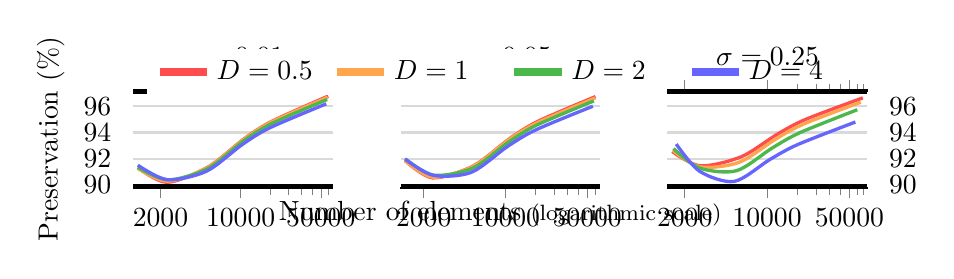
\begin{tikzpicture}
\begin{scope}[shift={(0.0\linewidth,0)}]
\begin{axis}[
 width=0.34\linewidth,height=0.23\linewidth,
 title=\normalsize\mbox{$\sigma=0.01$},
 xmode=log,enlarge x limits=0.025,
 ylabel=Preservation (\%),
 axis y line*=left,
 ymin=89.8717166667,ymax=97.1177141667,
 tick align=outside,
 x axis line style = ultra thick,y axis line style={white},
 xtick={2000,10000,50000},xticklabels={2000,10000,50000},
 minor xtick={18000,26000,34000,42000,58000,66000}, every y tick/.style={white},ymajorgrids,grid style={gray!30,thick}]
\addplot[very thick,mark=none,smooth,color=red!70] table[] {
	1269.16833333 91.3126666667
	2276.448 90.2003333333
	5182.04633333 91.3596666667
	10781.034 93.53
	18828.409 94.8593333333
	57983.79 96.7726666667
};
\addplot[very thick,mark=none,smooth,color=orange!70] table[] {
	1263.86633333 91.2736666667
	2291.61833333 90.285
	5160.89366667 91.328
	10724.269 93.4833333333
	18700.9823333 94.8033333333
	57488.1266667 96.687
};
\addplot[very thick,mark=none,smooth,color=green!60!black!70] table[] {
	1268.27666667 91.35
	2317.154 90.388
	5158.744 91.244
	10661.7936667 93.3703333333
	18531.0873333 94.6646666667
	56804.2343333 96.516
};
\addplot[very thick,mark=none,smooth,color=blue!60!] table[] {
	1271.49233333 91.503
	2295.37766667 90.4013333333
	5046.867 91.0493333333
	10420.654 93.102
	18138.199 94.3706666667
	55823.631 96.183
};
!\end{axis}
\end{scope}
\begin{scope}[shift={(0.28\linewidth,0)}]
\begin{axis}[
 width=0.34\linewidth,height=0.23\linewidth,
 title=\normalsize\mbox{$\sigma=0.05$},
 xmode=log,enlarge x limits=0.025,
 xlabel=Number of elements \footnotesize(logarithmic scale),x label style={at={(axis description cs:0.5,-0.05)},anchor=north},
 yticklabels={},
 legend style={at={(0.55,1.45)},legend style={text width=4em},legend style={draw=none},anchor=north,legend columns=-1},
 axis y line*=left,
 ymin=89.8717166667,ymax=97.1177141667,
 tick align=outside,
 x axis line style = ultra thick,y axis line style={white},
 xtick={2000,10000,50000},xticklabels={2000,10000,50000},
 minor xtick={18000,26000,34000,42000,58000,66000}, every y tick/.style={white},ymajorgrids,grid style={gray!30,thick}]
\addlegendimage{line width=3pt,mark=none,red!70}
\addlegendentry{$D=0.5$}
\addlegendimage{line width=3pt,mark=none,orange!70}
\addlegendentry{$D=1$}
\addlegendimage{line width=3pt,mark=none,green!60!black!70}
\addlegendentry{$D=2$}
\addlegendimage{line width=3pt,mark=none,blue!60!}
\addlegendentry{$D=4$}
\addplot[very thick,mark=none,smooth,color=red!70] table[] {
	1385.864 91.852
	2376.925 90.54
	5278.774 91.4403333333
	10966.038 93.558
	19097.6056667 94.865
	58814.4653333 96.7353333333
};
\addplot[very thick,mark=none,smooth,color=orange!70] table[] {
	1383.557 91.852
	2384.27766667 90.5893333333
	5254.04566667 91.3993333333
	10884.6076667 93.4913333333
	18943.0066667 94.768
	58423.8133333 96.626
};
\addplot[very thick,mark=none,smooth,color=green!60!black!70] table[] {
	1396.929 91.9713333333
	2419.80333333 90.7483333333
	5228.412 91.276
	10716.7823333 93.2896666667
	18603.7346667 94.57
	56994.5426667 96.4066666667
};
\addplot[very thick,mark=none,smooth,color=blue!60!] table[] {
	1381.061 91.9853333333
	2397.538 90.7393333333
	5081.389 90.9563333333
	10439.4216667 92.9413333333
	18174.898 94.1976666667
	55852.1183333 96.0006666667
};
!\end{axis}
\end{scope}
\begin{scope}[shift={(0.56\linewidth,0)}]
\begin{axis}[
 width=0.34\linewidth,height=0.23\linewidth,
 title=\normalsize\mbox{$\sigma=0.25$},
 xmode=log,enlarge x limits=0.025,
 axis y line*=right,
 ymin=89.8717166667,ymax=97.1177141667,
 tick align=outside,
 x axis line style = ultra thick,y axis line style={white},
 xtick={2000,10000,50000},xticklabels={2000,10000,50000},
 minor xtick={18000,26000,34000,42000,58000,66000}, every y tick/.style={white},ymajorgrids,grid style={gray!30,thick}]
\addplot[very thick,mark=none,smooth,color=red!70] table[] {
	1567.82 92.5526666667
	2702.218 91.4586666667
	6014.308 92.141
	12277.662 93.88
	21270.3676667 94.9986666667
	64968.27 96.637
};
\addplot[very thick,mark=none,smooth,color=orange!70] table[] {
	1588.167 92.6406666667
	2687.20233333 91.3796666667
	5771.60766667 91.7186666667
	11710.9023333 93.4676666667
	20285.6003333 94.6296666667
	62456.379 96.3103333333
};
\addplot[very thick,mark=none,smooth,color=green!60!black!70] table[] {
	1607.47966667 92.7696666667
	2683.991 91.286
	5506.855 91.086
	11072.7156667 92.8193333333
	19096.4883333 93.9936666667
	58285.7603333 95.732
};
\addplot[very thick,mark=none,smooth,color=blue!60!] table[] {
	1693.51233333 93.116
	2676.17366667 91.041
	5274.201 90.2713333333
	10604.068 91.9496666667
	18295.141 93.0873333333
	56172.5003333 94.795
};
!\end{axis}
\end{scope}
\end{tikzpicture}
\end{center}
\caption{Element preservation results using mesh remodelling - Clark-Y airfoil}\centering\sffamily\footnotesize
Average of thirty optimisation scenarios\end{figure}

\begin{figure}[!h]
\begin{center}
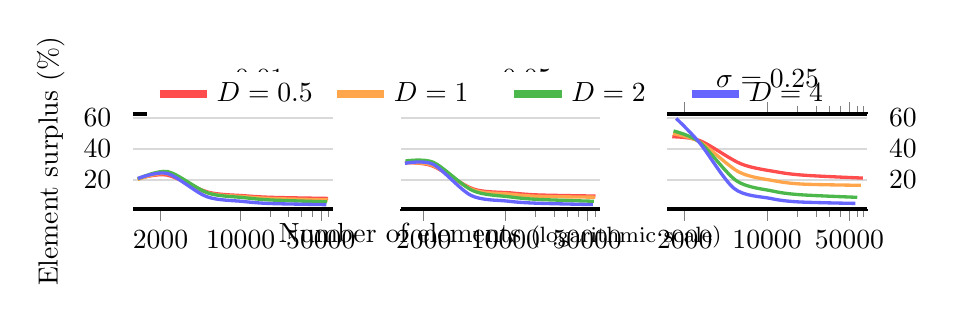
\begin{tikzpicture}
\begin{scope}[shift={(0.0\linewidth,0)}]
\begin{axis}[
 width=0.34\linewidth,height=0.23\linewidth,
 title=\normalsize\mbox{$\sigma=0.01$},
 xmode=log,enlarge x limits=0.025,
 ylabel=Element surplus (\%),
 axis y line*=left,
 ymin=1.09145085224,ymax=62.6174916048,
 tick align=outside,
 x axis line style = ultra thick,y axis line style={white},
 xtick={2000,10000,50000},xticklabels={2000,10000,50000},
 minor xtick={18000,26000,34000,42000,58000,66000}, every y tick/.style={white},ymajorgrids,grid style={gray!30,thick}]
\addplot[very thick,mark=none,smooth,color=red!70] table[] {
	1269.16833333 20.6488825853
	2276.448 23.0503120517
	5182.04633333 11.9998487086
	10781.034 9.63920601302
	18828.409 8.59936224928
	57983.79 7.9015700538
};
\addplot[very thick,mark=none,smooth,color=orange!70] table[] {
	1263.86633333 20.1448671929
	2291.61833333 23.8703238642
	5160.89366667 11.5426749757
	10724.269 9.06192654898
	18700.9823333 7.86438486836
	57488.1266667 6.97919412968
};
\addplot[very thick,mark=none,smooth,color=green!60!black!70] table[] {
	1268.27666667 20.5641195289
	2317.154 25.250619725
	5158.744 11.4962141133
	10661.7936667 8.42657506581
	18531.0873333 6.88445668381
	56804.2343333 5.70654436818
};
\addplot[very thick,mark=none,smooth,color=blue!60!] table[] {
	1271.49233333 20.8698052129
	2295.37766667 24.0735295337
	5046.867 9.07821043911
	10420.654 5.97427210566
	18138.199 4.61833730882
	55823.631 3.88174748501
};
!\end{axis}
\end{scope}
\begin{scope}[shift={(0.28\linewidth,0)}]
\begin{axis}[
 width=0.34\linewidth,height=0.23\linewidth,
 title=\normalsize\mbox{$\sigma=0.05$},
 xmode=log,enlarge x limits=0.025,
 xlabel=Number of elements \footnotesize(logarithmic scale),x label style={at={(axis description cs:0.5,-0.05)},anchor=north},
 yticklabels={},
 legend style={at={(0.55,1.45)},legend style={text width=4em},legend style={draw=none},anchor=north,legend columns=-1},
 axis y line*=left,
 ymin=1.09145085224,ymax=62.6174916048,
 tick align=outside,
 x axis line style = ultra thick,y axis line style={white},
 xtick={2000,10000,50000},xticklabels={2000,10000,50000},
 minor xtick={18000,26000,34000,42000,58000,66000}, every y tick/.style={white},ymajorgrids,grid style={gray!30,thick}]
\addlegendimage{line width=3pt,mark=none,red!70}
\addlegendentry{$D=0.5$}
\addlegendimage{line width=3pt,mark=none,orange!70}
\addlegendentry{$D=1$}
\addlegendimage{line width=3pt,mark=none,green!60!black!70}
\addlegendentry{$D=2$}
\addlegendimage{line width=3pt,mark=none,blue!60!}
\addlegendentry{$D=4$}
\addplot[very thick,mark=none,smooth,color=red!70] table[] {
	1385.864 31.0869587836
	2376.925 28.9324181874
	5278.774 14.0945389049
	10966.038 11.5141957066
	19097.6056667 10.1602245812
	58814.4653333 9.44232992405
};
\addplot[very thick,mark=none,smooth,color=orange!70] table[] {
	1383.557 30.8687428448
	2384.27766667 29.3312515934
	5254.04566667 13.5600648415
	10884.6076667 10.6861265235
	18943.0066667 9.26845517005
	58423.8133333 8.71540220606
};
\addplot[very thick,mark=none,smooth,color=green!60!black!70] table[] {
	1396.929 32.1335818281
	2419.80333333 31.2582834144
	5228.412 13.0060230548
	10716.7823333 8.97950221073
	18603.7346667 7.31144127174
	56994.5426667 6.05580628922
};
\addplot[very thick,mark=none,smooth,color=blue!60!] table[] {
	1381.061 30.6326496573
	2397.538 30.0505367381
	5081.389 9.8282925072
	10439.4216667 6.15900754676
	18174.898 4.83779382435
	55852.1183333 3.92997584779
};
!\end{axis}
\end{scope}
\begin{scope}[shift={(0.56\linewidth,0)}]
\begin{axis}[
 width=0.34\linewidth,height=0.23\linewidth,
 title=\normalsize\mbox{$\sigma=0.25$},
 xmode=log,enlarge x limits=0.025,
 axis y line*=right,
 ymin=1.09145085224,ymax=62.6174916048,
 tick align=outside,
 x axis line style = ultra thick,y axis line style={white},
 xtick={2000,10000,50000},xticklabels={2000,10000,50000},
 minor xtick={18000,26000,34000,42000,58000,66000}, every y tick/.style={white},ymajorgrids,grid style={gray!30,thick}]
\addplot[very thick,mark=none,smooth,color=red!70] table[] {
	1567.82 47.8356748574
	2702.218 45.2785068596
	6014.308 30.2691730707
	12277.662 24.9988537893
	21270.3676667 22.8580201517
	64968.27 21.0714976824
};
\addplot[very thick,mark=none,smooth,color=orange!70] table[] {
	1588.167 49.7542704082
	2687.20233333 44.4712242374
	5771.60766667 25.0123136402
	11710.9023333 19.2286746862
	20285.6003333 17.1699866029
	62456.379 16.3904679215
};
\addplot[very thick,mark=none,smooth,color=green!60!black!70] table[] {
	1607.47966667 51.5753347586
	2683.991 44.298574321
	5506.855 19.2778033765
	11072.7156667 12.7312974301
	19096.4883333 10.3016546423
	58285.7603333 8.61831932906
};
\addplot[very thick,mark=none,smooth,color=blue!60!] table[] {
	1693.51233333 59.6876801404
	2676.17366667 43.8782934575
	5274.201 14.238546293
	10604.068 7.95999641493
	18295.141 5.67305826025
	56172.5003333 4.68015762039
};
!\end{axis}
\end{scope}
\end{tikzpicture}
\end{center}
\caption{Element surplus results on meshes from mesh remodelling - Clark-Y airfoil}\centering\sffamily\footnotesize
Average of thirty optimisation scenarios\end{figure}

\begin{figure}[!h]
\begin{center}
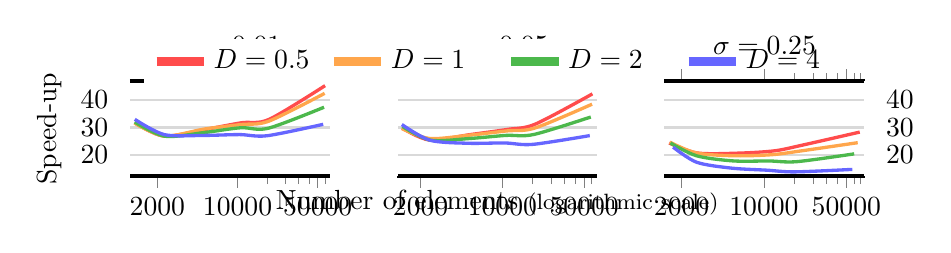
\begin{tikzpicture}
\begin{scope}[shift={(0.0\linewidth,0)}]
\begin{axis}[
 width=0.34\linewidth,height=0.23\linewidth,
 title=\normalsize\mbox{$\sigma=0.01$},
 xmode=log,enlarge x limits=0.025,
 ylabel=Speed-up,
 axis y line*=left,
 ymin=12.298001935,ymax=46.8477530579,
 tick align=outside,
 x axis line style = ultra thick,y axis line style={white},
 xtick={2000,10000,50000},xticklabels={2000,10000,50000},
 minor xtick={18000,26000,34000,42000,58000,66000}, every y tick/.style={white},ymajorgrids,grid style={gray!30,thick}]
\addplot[very thick,mark=none,smooth,color=red!70] table[] {
	1269.16833333 31.6855345912
	2276.448 26.8707707962
	5182.04633333 29.2477146264
	10781.034 31.7074162558
	18828.409 32.9383318154
	57983.79 45.202526814
};
\addplot[very thick,mark=none,smooth,color=orange!70] table[] {
	1263.86633333 31.6060225847
	2291.61833333 26.8776081425
	5160.89366667 29.4407881576
	10724.269 31.0678354418
	18700.9823333 32.2773651178
	57488.1266667 42.3926903045
};
\addplot[very thick,mark=none,smooth,color=green!60!black!70] table[] {
	1268.27666667 31.9670050761
	2317.154 26.8161970043
	5158.744 28.1727603369
	10661.7936667 29.8974309816
	18531.0873333 29.7190647863
	56804.2343333 37.3539723219
};
\addplot[very thick,mark=none,smooth,color=blue!60!] table[] {
	1271.49233333 32.9496402878
	2295.37766667 27.407628438
	5046.867 27.1089519248
	10420.654 27.4152858964
	18138.199 27.0006743413
	55823.631 31.1383365433
};
!\end{axis}
\end{scope}
\begin{scope}[shift={(0.28\linewidth,0)}]
\begin{axis}[
 width=0.34\linewidth,height=0.23\linewidth,
 title=\normalsize\mbox{$\sigma=0.05$},
 xmode=log,enlarge x limits=0.025,
 xlabel=Number of elements \footnotesize(logarithmic scale),x label style={at={(axis description cs:0.5,-0.05)},anchor=north},
 yticklabels={},
 legend style={at={(0.55,1.45)},legend style={text width=4em},legend style={draw=none},anchor=north,legend columns=-1},
 axis y line*=left,
 ymin=12.298001935,ymax=46.8477530579,
 tick align=outside,
 x axis line style = ultra thick,y axis line style={white},
 xtick={2000,10000,50000},xticklabels={2000,10000,50000},
 minor xtick={18000,26000,34000,42000,58000,66000}, every y tick/.style={white},ymajorgrids,grid style={gray!30,thick}]
\addlegendimage{line width=3pt,mark=none,red!70}
\addlegendentry{$D=0.5$}
\addlegendimage{line width=3pt,mark=none,orange!70}
\addlegendentry{$D=1$}
\addlegendimage{line width=3pt,mark=none,green!60!black!70}
\addlegendentry{$D=2$}
\addlegendimage{line width=3pt,mark=none,blue!60!}
\addlegendentry{$D=4$}
\addplot[very thick,mark=none,smooth,color=red!70] table[] {
	1385.864 29.8071005917
	2376.925 25.4262493935
	5278.774 27.4042288557
	10966.038 29.2777323652
	19097.6056667 31.2138004604
	58814.4653333 42.2111672218
};
\addplot[very thick,mark=none,smooth,color=orange!70] table[] {
	1383.557 29.5969447709
	2384.27766667 26.0002480774
	5254.04566667 27.2115713471
	10884.6076667 28.746943015
	18943.0066667 29.7920261508
	58423.8133333 38.4640840704
};
\addplot[very thick,mark=none,smooth,color=green!60!black!70] table[] {
	1396.929 30.3823884198
	2419.80333333 25.3892926357
	5228.412 25.9846684206
	10716.7823333 27.1159652639
	18603.7346667 27.459017608
	56994.5426667 33.8062258428
};
\addplot[very thick,mark=none,smooth,color=blue!60!] table[] {
	1381.061 31.075879087
	2397.538 25.3708545146
	5081.389 24.2571985095
	10439.4216667 24.367256283
	18174.898 23.8584241696
	55852.1183333 27.0495972092
};
!\end{axis}
\end{scope}
\begin{scope}[shift={(0.56\linewidth,0)}]
\begin{axis}[
 width=0.34\linewidth,height=0.23\linewidth,
 title=\normalsize\mbox{$\sigma=0.25$},
 xmode=log,enlarge x limits=0.025,
 axis y line*=right,
 ymin=12.298001935,ymax=46.8477530579,
 tick align=outside,
 x axis line style = ultra thick,y axis line style={white},
 xtick={2000,10000,50000},xticklabels={2000,10000,50000},
 minor xtick={18000,26000,34000,42000,58000,66000}, every y tick/.style={white},ymajorgrids,grid style={gray!30,thick}]
\addplot[very thick,mark=none,smooth,color=red!70] table[] {
	1567.82 24.3597087379
	2702.218 20.7384125721
	6014.308 20.6685714286
	12277.662 21.5144055236
	21270.3676667 23.5989934336
	64968.27 28.321400669
};
\addplot[very thick,mark=none,smooth,color=orange!70] table[] {
	1588.167 24.6710914454
	2687.20233333 20.6931321953
	5771.60766667 19.7048959955
	11710.9023333 20.1133153092
	20285.6003333 21.433680576
	62456.379 24.4699482658
};
\addplot[very thick,mark=none,smooth,color=green!60!black!70] table[] {
	1607.47966667 24.3478893741
	2683.991 19.6924820552
	5506.855 17.8394183961
	11072.7156667 17.8210863576
	19096.4883333 17.5816127838
	58285.7603333 20.4091672825
};
\addplot[very thick,mark=none,smooth,color=blue!60!] table[] {
	1693.51233333 22.8510928962
	2676.17366667 17.372437927
	5274.201 15.234055355
	10604.068 14.470046195
	18295.141 13.8648840721
	56172.5003333 14.7614343841
};
!\end{axis}
\end{scope}
\end{tikzpicture}
\end{center}
\caption{Speed-up results by mesh remodelling - Clark-Y airfoil}\centering\sffamily\footnotesize
Average of thirty optimisation scenarios\end{figure}

\pagebreak
\subsubsection{Boeing 737}
\vspace*{\fill} \begin{table}[!hp]
\begin{center}
\begin{tabular}{c|cc?c|c?c?c|c|c||c|c}
\multirow{2}{*}{\textbf{\large $\boldsymbol{\sigma}$}} & \multirow{2}{*}{\textbf{\large $\boldsymbol{I}$}} & \multirow{2}{*}{\textbf{\large $\boldsymbol{G}$}} & \multicolumn{2}{c?}{\textbf{\large Generation}} & \multirow{2}{*}{\textbf{\large $\boldsymbol{D}$}} & \multicolumn{5}{c}{\textbf{{\large Remodelling} }} \\\cline{4-5}\cline{7-11}
 & & & \textbf{\# Tri.} & \textbf{Time} & &\textbf{\# Tri.} & \textbf{Time} & \textbf{Preserv.} & \textbf{+ Tri.} & \textbf{Sp.-up} \\\toprule
\multirow{24}[11]{*}{.01} & \multirow{4}{*}{50} & \multirow{4}{*}{1} & \multirow{4}{*}{1167} & \multirow{4}{*}{1.78 ms} & .5 & 1182 & 0.05 ms & 90.97 \% & 1.24 \% & 34.92 \\\cline{6-11}
 & & & &  & 1 & 1182 & 0.05 ms & 90.97 \% & 1.24 \% & 34.99 \\\cline{6-11}
 & & & &  & 2 & 1184 & 0.05 ms & 90.99 \% & 1.47 \% & 35.11 \\\cline{6-11}
 & & & &  & 4 & 1192 & 0.05 ms & 91.15 \% & 2.11 \% & 36.38 \\\cmidrule[1.5pt]{2-11}
 & \multirow{4}{*}{100} & \multirow{4}{*}{2} & \multirow{4}{*}{1864} & \multirow{4}{*}{3.42 ms} & .5 & 2215 & 0.12 ms & 89.98 \% & 18.86 \% & 27.65 \\\cline{6-11}
 & & & &  & 1 & 2217 & 0.12 ms & 90.00 \% & 18.95 \% & 27.64 \\\cline{6-11}
 & & & &  & 2 & 2229 & 0.12 ms & 90.07 \% & 19.60 \% & 27.86 \\\cline{6-11}
 & & & &  & 4 & 2228 & 0.12 ms & 90.19 \% & 19.53 \% & 28.44 \\\cmidrule[1.5pt]{2-11}
 & \multirow{4}{*}{200} & \multirow{4}{*}{4} & \multirow{4}{*}{4716} & \multirow{4}{*}{9.56 ms} & .5 & 5182 & 0.32 ms & 91.46 \% & 9.87 \% & 30.26 \\\cline{6-11}
 & & & &  & 1 & 5156 & 0.31 ms & 91.43 \% & 9.32 \% & 30.80 \\\cline{6-11}
 & & & &  & 2 & 5150 & 0.32 ms & 91.38 \% & 9.21 \% & 29.66 \\\cline{6-11}
 & & & &  & 4 & 5054 & 0.31 ms & 91.30 \% & 7.16 \% & 30.63 \\\cmidrule[1.5pt]{2-11}
 & \multirow{4}{*}{300} & \multirow{4}{*}{6} & \multirow{4}{*}{9982} & \multirow{4}{*}{20.06 ms} & .5 & 10894 & 0.62 ms & 93.71 \% & 9.14 \% & 32.25 \\\cline{6-11}
 & & & &  & 1 & 10845 & 0.63 ms & 93.66 \% & 8.65 \% & 32.01 \\\cline{6-11}
 & & & &  & 2 & 10788 & 0.66 ms & 93.60 \% & 8.08 \% & 30.42 \\\cline{6-11}
 & & & &  & 4 & 10584 & 0.68 ms & 93.45 \% & 6.04 \% & 29.38 \\\cmidrule[1.5pt]{2-11}
 & \multirow{4}{*}{400} & \multirow{4}{*}{8} & \multirow{4}{*}{17626} & \multirow{4}{*}{36.61 ms} & .5 & 19120 & 1.09 ms & 95.04 \% & 8.47 \% & 33.47 \\\cline{6-11}
 & & & &  & 1 & 18986 & 1.11 ms & 94.99 \% & 7.71 \% & 32.94 \\\cline{6-11}
 & & & &  & 2 & 18838 & 1.17 ms & 94.90 \% & 6.88 \% & 31.31 \\\cline{6-11}
 & & & &  & 4 & 18490 & 1.25 ms & 94.72 \% & 4.90 \% & 29.31 \\\cmidrule[1.5pt]{2-11}
 & \multirow{4}{*}{700} & \multirow{4}{*}{14} & \multirow{4}{*}{54768} & \multirow{4}{*}{158.33 ms} & .5 & 59055 & 3.31 ms & 96.89 \% & 7.83 \% & 47.84 \\\cline{6-11}
 & & & &  & 1 & 58578 & 3.44 ms & 96.84 \% & 6.96 \% & 45.97 \\\cline{6-11}
 & & & &  & 2 & 57903 & 3.71 ms & 96.73 \% & 5.72 \% & 42.68 \\\cline{6-11}
 & & & &  & 4 & 56903 & 4.32 ms & 96.51 \% & 3.90 \% & 36.68\\\bottomrule
\end{tabular}\end{center}
\caption{Full results of mesh remodelling for $\sigma=0.01$ - Boeing 737 airfoil}\centering\sffamily\footnotesize
Average of thirty optimisation scenarios\end{table}
 \vspace*{\fill}
\begin{table}[!hp]
\begin{center}
\begin{tabular}{c|cc?c|c?c?c|c|c||c|c}
\multirow{2}{*}{\textbf{\large $\boldsymbol{\sigma}$}} & \multirow{2}{*}{\textbf{\large $\boldsymbol{I}$}} & \multirow{2}{*}{\textbf{\large $\boldsymbol{G}$}} & \multicolumn{2}{c?}{\textbf{\large Generation}} & \multirow{2}{*}{\textbf{\large $\boldsymbol{D}$}} & \multicolumn{5}{c}{\textbf{{\large Remodelling} }} \\\cline{4-5}\cline{7-11}
 & & & \textbf{\# Tri.} & \textbf{Time} & &\textbf{\# Tri.} & \textbf{Time} & \textbf{Preserv.} & \textbf{+ Tri.} & \textbf{Sp.-up} \\\toprule
\multirow{24}[13]{*}{.05} & \multirow{4}{*}{50} & \multirow{4}{*}{1} & \multirow{4}{*}{1165} & \multirow{4}{*}{1.78 ms} & .5 & 1280 & 0.05 ms & 91.48 \% & 9.81 \% & 33.55 \\\cline{6-11}
 & & & &  & 1 & 1279 & 0.05 ms & 91.47 \% & 9.73 \% & 33.46 \\\cline{6-11}
 & & & &  & 2 & 1317 & 0.05 ms & 91.71 \% & 12.99 \% & 34.04 \\\cline{6-11}
 & & & &  & 4 & 1310 & 0.05 ms & 91.78 \% & 12.44 \% & 34.50 \\\cmidrule[1.5pt]{2-11}
 & \multirow{4}{*}{100} & \multirow{4}{*}{2} & \multirow{4}{*}{1864} & \multirow{4}{*}{3.41 ms} & .5 & 2390 & 0.13 ms & 90.59 \% & 28.20 \% & 25.95 \\\cline{6-11}
 & & & &  & 1 & 2411 & 0.13 ms & 90.67 \% & 29.31 \% & 26.13 \\\cline{6-11}
 & & & &  & 2 & 2404 & 0.13 ms & 90.69 \% & 28.93 \% & 26.03 \\\cline{6-11}
 & & & &  & 4 & 2416 & 0.13 ms & 90.83 \% & 29.58 \% & 26.55 \\\cmidrule[1.5pt]{2-11}
 & \multirow{4}{*}{200} & \multirow{4}{*}{4} & \multirow{4}{*}{4717} & \multirow{4}{*}{9.20 ms} & .5 & 5291 & 0.34 ms & 91.50 \% & 12.16 \% & 27.31 \\\cline{6-11}
 & & & &  & 1 & 5293 & 0.34 ms & 91.50 \% & 12.20 \% & 26.80 \\\cline{6-11}
 & & & &  & 2 & 5296 & 0.35 ms & 91.46 \% & 12.27 \% & 26.09 \\\cline{6-11}
 & & & &  & 4 & 5161 & 0.36 ms & 91.27 \% & 9.41 \% & 25.91 \\\cmidrule[1.5pt]{2-11}
 & \multirow{4}{*}{300} & \multirow{4}{*}{6} & \multirow{4}{*}{9982} & \multirow{4}{*}{19.73 ms} & .5 & 11085 & 0.69 ms & 93.68 \% & 11.06 \% & 28.43 \\\cline{6-11}
 & & & &  & 1 & 11011 & 0.70 ms & 93.63 \% & 10.31 \% & 28.25 \\\cline{6-11}
 & & & &  & 2 & 10928 & 0.73 ms & 93.54 \% & 9.48 \% & 27.21 \\\cline{6-11}
 & & & &  & 4 & 10652 & 0.77 ms & 93.27 \% & 6.71 \% & 25.47 \\\cmidrule[1.5pt]{2-11}
 & \multirow{4}{*}{400} & \multirow{4}{*}{8} & \multirow{4}{*}{17627} & \multirow{4}{*}{36.40 ms} & .5 & 19376 & 1.22 ms & 94.97 \% & 9.92 \% & 29.74 \\\cline{6-11}
 & & & &  & 1 & 19272 & 1.25 ms & 94.92 \% & 9.33 \% & 29.20 \\\cline{6-11}
 & & & &  & 2 & 18999 & 1.32 ms & 94.79 \% & 7.78 \% & 27.49 \\\cline{6-11}
 & & & &  & 4 & 18521 & 1.46 ms & 94.50 \% & 5.07 \% & 24.99 \\\cmidrule[1.5pt]{2-11}
 & \multirow{4}{*}{700} & \multirow{4}{*}{14} & \multirow{4}{*}{54755} & \multirow{4}{*}{157.51 ms} & .5 & 59893 & 3.69 ms & 96.82 \% & 9.38 \% & 42.66 \\\cline{6-11}
 & & & &  & 1 & 59538 & 3.96 ms & 96.74 \% & 8.74 \% & 39.81 \\\cline{6-11}
 & & & &  & 2 & 58279 & 4.30 ms & 96.60 \% & 6.44 \% & 36.62 \\\cline{6-11}
 & & & &  & 4 & 56986 & 5.19 ms & 96.27 \% & 4.08 \% & 30.35\\\bottomrule
\end{tabular}\end{center}
\caption{Full results of mesh remodelling for $\sigma=0.05$ - Boeing 737 airfoil}\centering\sffamily\footnotesize
Average of thirty optimisation scenarios\end{table}

\begin{table}[!hp]
\begin{center}
\begin{tabular}{c|cc?c|c?c?c|c|c||c|c}
\multirow{2}{*}{\textbf{\large $\boldsymbol{\sigma}$}} & \multirow{2}{*}{\textbf{\large $\boldsymbol{I}$}} & \multirow{2}{*}{\textbf{\large $\boldsymbol{G}$}} & \multicolumn{2}{c?}{\textbf{\large Generation}} & \multirow{2}{*}{\textbf{\large $\boldsymbol{D}$}} & \multicolumn{5}{c}{\textbf{{\large Remodelling} }} \\\cline{4-5}\cline{7-11}
 & & & \textbf{\# Tri.} & \textbf{Time} & &\textbf{\# Tri.} & \textbf{Time} & \textbf{Preserv.} & \textbf{+ Tri.} & \textbf{Sp.-up} \\\toprule
\multirow{24}[13]{*}{.25} & \multirow{4}{*}{50} & \multirow{4}{*}{1} & \multirow{4}{*}{1172} & \multirow{4}{*}{1.78 ms} & .5 & 1646 & 0.07 ms & 92.82 \% & 40.50 \% & 26.26 \\\cline{6-11}
 & & & &  & 1 & 1663 & 0.07 ms & 92.94 \% & 41.94 \% & 25.52 \\\cline{6-11}
 & & & &  & 2 & 1689 & 0.07 ms & 92.99 \% & 44.13 \% & 25.79 \\\cline{6-11}
 & & & &  & 4 & 1801 & 0.08 ms & 93.38 \% & 53.73 \% & 23.76 \\\cmidrule[1.5pt]{2-11}
 & \multirow{4}{*}{100} & \multirow{4}{*}{2} & \multirow{4}{*}{1859} & \multirow{4}{*}{3.39 ms} & .5 & 2810 & 0.17 ms & 91.71 \% & 51.15 \% & 20.31 \\\cline{6-11}
 & & & &  & 1 & 2790 & 0.17 ms & 91.62 \% & 50.07 \% & 19.89 \\\cline{6-11}
 & & & &  & 2 & 2773 & 0.18 ms & 91.48 \% & 49.11 \% & 19.13 \\\cline{6-11}
 & & & &  & 4 & 2773 & 0.20 ms & 91.23 \% & 49.14 \% & 16.82 \\\cmidrule[1.5pt]{2-11}
 & \multirow{4}{*}{200} & \multirow{4}{*}{4} & \multirow{4}{*}{4715} & \multirow{4}{*}{9.06 ms} & .5 & 6177 & 0.45 ms & 92.32 \% & 31.02 \% & 19.92 \\\cline{6-11}
 & & & &  & 1 & 5894 & 0.47 ms & 91.88 \% & 25.02 \% & 19.37 \\\cline{6-11}
 & & & &  & 2 & 5655 & 0.52 ms & 91.28 \% & 19.94 \% & 17.57 \\\cline{6-11}
 & & & &  & 4 & 5387 & 0.60 ms & 90.45 \% & 14.26 \% & 15.04 \\\cmidrule[1.5pt]{2-11}
 & \multirow{4}{*}{300} & \multirow{4}{*}{6} & \multirow{4}{*}{9974} & \multirow{4}{*}{19.53 ms} & .5 & 12514 & 0.92 ms & 94.00 \% & 25.47 \% & 21.22 \\\cline{6-11}
 & & & &  & 1 & 11932 & 0.99 ms & 93.59 \% & 19.63 \% & 19.82 \\\cline{6-11}
 & & & &  & 2 & 11316 & 1.11 ms & 92.97 \% & 13.45 \% & 17.57 \\\cline{6-11}
 & & & &  & 4 & 10820 & 1.36 ms & 92.10 \% & 8.48 \% & 14.34 \\\cmidrule[1.5pt]{2-11}
 & \multirow{4}{*}{400} & \multirow{4}{*}{8} & \multirow{4}{*}{17610} & \multirow{4}{*}{36.04 ms} & .5 & 21685 & 1.57 ms & 95.09 \% & 23.14 \% & 22.99 \\\cline{6-11}
 & & & &  & 1 & 20686 & 1.72 ms & 94.71 \% & 17.47 \% & 20.99 \\\cline{6-11}
 & & & &  & 2 & 19525 & 2.03 ms & 94.11 \% & 10.87 \% & 17.78 \\\cline{6-11}
 & & & &  & 4 & 18649 & 2.62 ms & 93.21 \% & 5.90 \% & 13.78 \\\cmidrule[1.5pt]{2-11}
 & \multirow{4}{*}{700} & \multirow{4}{*}{14} & \multirow{4}{*}{54727} & \multirow{4}{*}{156.47 ms} & .5 & 66406 & 5.46 ms & 96.69 \% & 21.34 \% & 28.66 \\\cline{6-11}
 & & & &  & 1 & 63703 & 6.31 ms & 96.35 \% & 16.40 \% & 24.80 \\\cline{6-11}
 & & & &  & 2 & 59598 & 7.52 ms & 95.81 \% & 8.90 \% & 20.82 \\\cline{6-11}
 & & & &  & 4 & 57326 & 10.38 ms & 94.88 \% & 4.75 \% & 15.08\\\bottomrule
\end{tabular}\end{center}
\caption{Full results of mesh remodelling for $\sigma=0.25$ - Boeing 737 airfoil}\centering\sffamily\footnotesize
Average of thirty optimisation scenarios\end{table}
 \newpage
\begin{figure}[!h]
\begin{center}
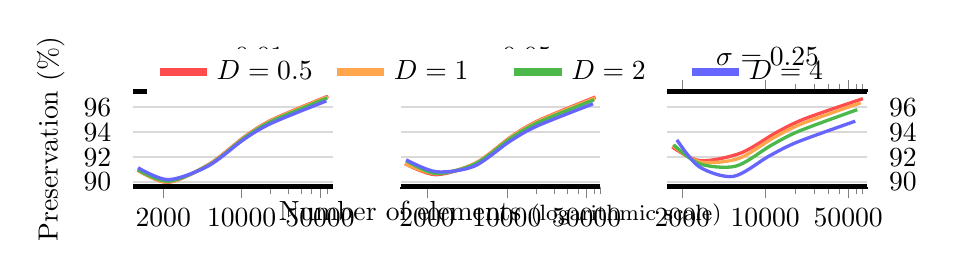
\begin{tikzpicture}
\begin{scope}[shift={(0.0\linewidth,0)}]
\begin{axis}[
 width=0.34\linewidth,height=0.23\linewidth,
 title=\normalsize\mbox{$\sigma=0.01$},
 xmode=log,enlarge x limits=0.025,
 ylabel=Preservation (\%),
 axis y line*=left,
 ymin=89.635,ymax=97.25695,
 tick align=outside,
 x axis line style = ultra thick,y axis line style={white},
 xtick={2000,10000,50000},xticklabels={2000,10000,50000},
 minor xtick={18000,26000,34000,42000,58000,66000}, every y tick/.style={white},ymajorgrids,grid style={gray!30,thick}]
\addplot[very thick,mark=none,smooth,color=red!70] table[] {
	1181.62066667 90.969
	2215.46 89.9806666667
	5181.616 91.459
	10893.6296667 93.7076666667
	19119.5003333 95.038
	59054.826 96.894
};
\addplot[very thick,mark=none,smooth,color=orange!70] table[] {
	1181.62066667 90.969
	2217.06433333 90.001
	5155.626 91.4273333333
	10845.362 93.662
	18986.0146667 94.9903333333
	58578.4676667 96.8403333333
};
\addplot[very thick,mark=none,smooth,color=green!60!black!70] table[] {
	1184.32666667 90.989
	2229.279 90.0676666667
	5150.313 91.38
	10787.995 93.599
	18838.031 94.905
	57902.6766667 96.7316666667
};
\addplot[very thick,mark=none,smooth,color=blue!60!] table[] {
	1191.78133333 91.146
	2227.87566667 90.1936666667
	5053.76633333 91.3006666667
	10584.265 93.4486666667
	18489.5223333 94.724
	56902.9196667 96.5066666667
};
!\end{axis}
\end{scope}
\begin{scope}[shift={(0.28\linewidth,0)}]
\begin{axis}[
 width=0.34\linewidth,height=0.23\linewidth,
 title=\normalsize\mbox{$\sigma=0.05$},
 xmode=log,enlarge x limits=0.025,
 xlabel=Number of elements \footnotesize(logarithmic scale),x label style={at={(axis description cs:0.5,-0.05)},anchor=north},
 yticklabels={},
 legend style={at={(0.55,1.45)},legend style={text width=4em},legend style={draw=none},anchor=north,legend columns=-1},
 axis y line*=left,
 ymin=89.635,ymax=97.25695,
 tick align=outside,
 x axis line style = ultra thick,y axis line style={white},
 xtick={2000,10000,50000},xticklabels={2000,10000,50000},
 minor xtick={18000,26000,34000,42000,58000,66000}, every y tick/.style={white},ymajorgrids,grid style={gray!30,thick}]
\addlegendimage{line width=3pt,mark=none,red!70}
\addlegendentry{$D=0.5$}
\addlegendimage{line width=3pt,mark=none,orange!70}
\addlegendentry{$D=1$}
\addlegendimage{line width=3pt,mark=none,green!60!black!70}
\addlegendentry{$D=2$}
\addlegendimage{line width=3pt,mark=none,blue!60!}
\addlegendentry{$D=4$}
\addplot[very thick,mark=none,smooth,color=red!70] table[] {
	1279.641 91.4773333333
	2390.32533333 90.5906666667
	5290.78533333 91.504
	11085.4573333 93.683
	19376.218 94.9713333333
	59892.9113333 96.8196666667
};
\addplot[very thick,mark=none,smooth,color=orange!70] table[] {
	1278.69166667 91.4746666667
	2410.959 90.6716666667
	5292.737 91.501
	11011.373 93.633
	19272.0743333 94.9203333333
	59537.7083333 96.7386666667
};
\addplot[very thick,mark=none,smooth,color=green!60!black!70] table[] {
	1316.78633333 91.7136666667
	2403.786 90.687
	5295.75033333 91.459
	10928.2076667 93.538
	18998.6893333 94.7936666667
	58278.8796667 96.599
};
\addplot[very thick,mark=none,smooth,color=blue!60!] table[] {
	1310.299 91.7836666667
	2415.94733333 90.8263333333
	5160.93433333 91.268
	10652.052 93.2716666667
	18520.5773333 94.5046666667
	56986.4536667 96.2736666667
};
!\end{axis}
\end{scope}
\begin{scope}[shift={(0.56\linewidth,0)}]
\begin{axis}[
 width=0.34\linewidth,height=0.23\linewidth,
 title=\normalsize\mbox{$\sigma=0.25$},
 xmode=log,enlarge x limits=0.025,
 axis y line*=right,
 ymin=89.635,ymax=97.25695,
 tick align=outside,
 x axis line style = ultra thick,y axis line style={white},
 xtick={2000,10000,50000},xticklabels={2000,10000,50000},
 minor xtick={18000,26000,34000,42000,58000,66000}, every y tick/.style={white},ymajorgrids,grid style={gray!30,thick}]
\addplot[very thick,mark=none,smooth,color=red!70] table[] {
	1646.15933333 92.8183333333
	2810.362 91.7126666667
	6177.13333333 92.3163333333
	12514.3133333 93.997
	21685.3016667 95.088
	66406.0556667 96.6856666667
};
\addplot[very thick,mark=none,smooth,color=orange!70] table[] {
	1663.08533333 92.936
	2790.36366667 91.6196666667
	5894.47266667 91.875
	11932.3566667 93.5886666667
	20686.2586667 94.706
	63703.007 96.3536666667
};
\addplot[very thick,mark=none,smooth,color=green!60!black!70] table[] {
	1688.79933333 92.9936666667
	2772.61566667 91.4773333333
	5654.935 91.2786666667
	11315.806 92.968
	19524.696 94.1093333333
	59597.5723333 95.8066666667
};
\addplot[very thick,mark=none,smooth,color=blue!60!] table[] {
	1801.26033333 93.3823333333
	2773.10966667 91.2313333333
	5387.17566667 90.4546666667
	10819.9246667 92.096
	18649.48 93.2103333333
	57325.7383333 94.8823333333
};
!\end{axis}
\end{scope}
\end{tikzpicture}
\end{center}
\caption{Element preservation results using mesh remodelling - Boeing 737 airfoil}\centering\sffamily\footnotesize
Average of thirty optimisation scenarios\end{figure}

\begin{figure}[!h]
\begin{center}
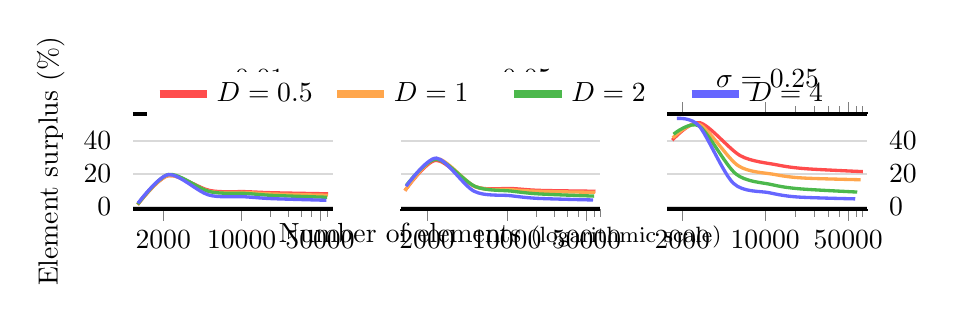
\begin{tikzpicture}
\begin{scope}[shift={(0.0\linewidth,0)}]
\begin{axis}[
 width=0.34\linewidth,height=0.23\linewidth,
 title=\normalsize\mbox{$\sigma=0.01$},
 xmode=log,enlarge x limits=0.025,
 ylabel=Element surplus (\%),
 axis y line*=left,
 ymin=-1.38849385705,ymax=56.4888893543,
 tick align=outside,
 x axis line style = ultra thick,y axis line style={white},
 xtick={2000,10000,50000},xticklabels={2000,10000,50000},
 minor xtick={18000,26000,34000,42000,58000,66000}, every y tick/.style={white},ymajorgrids,grid style={gray!30,thick}]
\addplot[very thick,mark=none,smooth,color=red!70] table[] {
	1181.62066667 1.23633077838
	2215.46 18.8601239751
	5181.616 9.8721420683
	10893.6296667 9.13811486868
	19119.5003333 8.47199379817
	59054.826 7.82769866292
};
\addplot[very thick,mark=none,smooth,color=orange!70] table[] {
	1181.62066667 1.23633077838
	2217.06433333 18.9461969617
	5155.626 9.32104430799
	10845.362 8.65454398273
	18986.0146667 7.71468026203
	58578.4676667 6.95792008086
};
\addplot[very thick,mark=none,smooth,color=green!60!black!70] table[] {
	1184.32666667 1.46816957303
	2229.279 19.6015176601
	5150.313 9.20838627027
	10787.995 8.07981118685
	18838.031 6.87511421202
	57902.6766667 5.72399910872
};
\addplot[very thick,mark=none,smooth,color=blue!60!] table[] {
	1191.78133333 2.10685432339
	2227.87566667 19.5262283865
	5053.76633333 7.16118920352
	10584.265 6.03873683215
	18489.5223333 4.89789570368
	56902.9196667 3.89855140472
};
!\end{axis}
\end{scope}
\begin{scope}[shift={(0.28\linewidth,0)}]
\begin{axis}[
 width=0.34\linewidth,height=0.23\linewidth,
 title=\normalsize\mbox{$\sigma=0.05$},
 xmode=log,enlarge x limits=0.025,
 xlabel=Number of elements \footnotesize(logarithmic scale),x label style={at={(axis description cs:0.5,-0.05)},anchor=north},
 yticklabels={},
 legend style={at={(0.55,1.45)},legend style={text width=4em},legend style={draw=none},anchor=north,legend columns=-1},
 axis y line*=left,
 ymin=-1.38849385705,ymax=56.4888893543,
 tick align=outside,
 x axis line style = ultra thick,y axis line style={white},
 xtick={2000,10000,50000},xticklabels={2000,10000,50000},
 minor xtick={18000,26000,34000,42000,58000,66000}, every y tick/.style={white},ymajorgrids,grid style={gray!30,thick}]
\addlegendimage{line width=3pt,mark=none,red!70}
\addlegendentry{$D=0.5$}
\addlegendimage{line width=3pt,mark=none,orange!70}
\addlegendentry{$D=1$}
\addlegendimage{line width=3pt,mark=none,green!60!black!70}
\addlegendentry{$D=2$}
\addlegendimage{line width=3pt,mark=none,blue!60!}
\addlegendentry{$D=4$}
\addplot[very thick,mark=none,smooth,color=red!70] table[] {
	1279.641 9.80665460552
	2390.32533333 28.2047908097
	5290.78533333 12.1616006639
	11085.4573333 11.0568597014
	19376.218 9.92389130736
	59892.9113333 9.3842464256
};
\addplot[very thick,mark=none,smooth,color=orange!70] table[] {
	1278.69166667 9.72519182226
	2410.959 29.3114748588
	5292.737 12.2029748727
	11011.373 10.3146644842
	19272.0743333 9.33307027639
	59537.7083333 8.73552837837
};
\addplot[very thick,mark=none,smooth,color=green!60!black!70] table[] {
	1316.78633333 12.9941148288
	2403.786 28.9267519294
	5295.75033333 12.2668558032
	10928.2076667 9.4814935578
	18998.6893333 7.78212039416
	58278.8796667 6.43649128004
};
\addplot[very thick,mark=none,smooth,color=blue!60!] table[] {
	1310.299 12.4374334075
	2415.94733333 29.5790234735
	5160.93433333 9.40883428043
	10652.052 6.71489762887
	18520.5773333 5.06972669996
	56986.4536667 4.07609434952
};
!\end{axis}
\end{scope}
\begin{scope}[shift={(0.56\linewidth,0)}]
\begin{axis}[
 width=0.34\linewidth,height=0.23\linewidth,
 title=\normalsize\mbox{$\sigma=0.25$},
 xmode=log,enlarge x limits=0.025,
 axis y line*=right,
 ymin=-1.38849385705,ymax=56.4888893543,
 tick align=outside,
 x axis line style = ultra thick,y axis line style={white},
 xtick={2000,10000,50000},xticklabels={2000,10000,50000},
 minor xtick={18000,26000,34000,42000,58000,66000}, every y tick/.style={white},ymajorgrids,grid style={gray!30,thick}]
\addplot[very thick,mark=none,smooth,color=red!70] table[] {
	1646.15933333 40.4953617974
	2810.362 51.1450315992
	6177.13333333 31.0158454274
	12514.3133333 25.4674709279
	21685.3016667 23.140689939
	66406.0556667 21.3397524168
};
\addplot[very thick,mark=none,smooth,color=orange!70] table[] {
	1663.08533333 41.9399513008
	2790.36366667 50.0694944536
	5894.47266667 25.0206654282
	11932.3566667 19.632821498
	20686.2586667 17.4675918107
	63703.007 16.400635755
};
\addplot[very thick,mark=none,smooth,color=green!60!black!70] table[] {
	1688.79933333 44.1345734495
	2772.61566667 49.114983248
	5654.935 19.9401162128
	11315.806 13.4513354839
	19524.696 10.8716204758
	59597.5723333 8.89902432793
};
\addplot[very thick,mark=none,smooth,color=blue!60!] table[] {
	1801.26033333 53.7328234871
	2773.10966667 49.1415512295
	5387.17566667 14.2609907132
	10819.9246667 8.4796702302
	18649.48 5.90167798931
	57325.7383333 4.74784003721
};
!\end{axis}
\end{scope}
\end{tikzpicture}
\end{center}
\caption{Element surplus results on meshes from mesh remodelling - Boeing 737 airfoil}\centering\sffamily\footnotesize
Average of thirty optimisation scenarios\end{figure}

\begin{figure}[!h]
\begin{center}
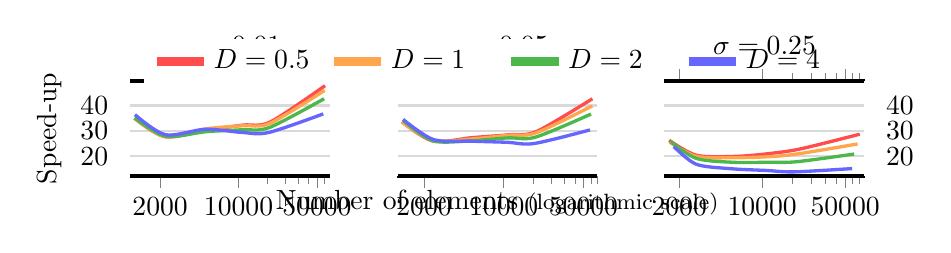
\begin{tikzpicture}
\begin{scope}[shift={(0.0\linewidth,0)}]
\begin{axis}[
 width=0.34\linewidth,height=0.23\linewidth,
 title=\normalsize\mbox{$\sigma=0.01$},
 xmode=log,enlarge x limits=0.025,
 ylabel=Speed-up,
 axis y line*=left,
 ymin=12.0793620886,ymax=49.6291431477,
 tick align=outside,
 x axis line style = ultra thick,y axis line style={white},
 xtick={2000,10000,50000},xticklabels={2000,10000,50000},
 minor xtick={18000,26000,34000,42000,58000,66000}, every y tick/.style={white},ymajorgrids,grid style={gray!30,thick}]
\addplot[very thick,mark=none,smooth,color=red!70] table[] {
	1181.62066667 34.9247874428
	2215.46 27.6488159311
	5181.616 30.264035458
	10893.6296667 32.2484055952
	19119.5003333 33.4710920118
	59054.826 47.8410583353
};
\addplot[very thick,mark=none,smooth,color=orange!70] table[] {
	1181.62066667 34.9934469201
	2217.06433333 27.6413774549
	5155.626 30.7970360825
	10845.362 32.0099478668
	18986.0146667 32.9400119976
	58578.4676667 45.9683063494
};
\addplot[very thick,mark=none,smooth,color=green!60!black!70] table[] {
	1184.32666667 35.1084812623
	2229.279 27.8587310195
	5150.313 29.6630119983
	10787.995 30.4238547881
	18838.031 31.3061573546
	57902.6766667 42.6751507093
};
\addplot[very thick,mark=none,smooth,color=blue!60!] table[] {
	1191.78133333 36.3760217984
	2227.87566667 28.4449058693
	5053.76633333 30.6260145237
	10584.265 29.3838753785
	18489.5223333 29.3124432819
	56902.9196667 36.6790190189
};
!\end{axis}
\end{scope}
\begin{scope}[shift={(0.28\linewidth,0)}]
\begin{axis}[
 width=0.34\linewidth,height=0.23\linewidth,
 title=\normalsize\mbox{$\sigma=0.05$},
 xmode=log,enlarge x limits=0.025,
 xlabel=Number of elements \footnotesize(logarithmic scale),x label style={at={(axis description cs:0.5,-0.05)},anchor=north},
 yticklabels={},
 legend style={at={(0.55,1.45)},legend style={text width=4em},legend style={draw=none},anchor=north,legend columns=-1},
 axis y line*=left,
 ymin=12.0793620886,ymax=49.6291431477,
 tick align=outside,
 x axis line style = ultra thick,y axis line style={white},
 xtick={2000,10000,50000},xticklabels={2000,10000,50000},
 minor xtick={18000,26000,34000,42000,58000,66000}, every y tick/.style={white},ymajorgrids,grid style={gray!30,thick}]
\addlegendimage{line width=3pt,mark=none,red!70}
\addlegendentry{$D=0.5$}
\addlegendimage{line width=3pt,mark=none,orange!70}
\addlegendentry{$D=1$}
\addlegendimage{line width=3pt,mark=none,green!60!black!70}
\addlegendentry{$D=2$}
\addlegendimage{line width=3pt,mark=none,blue!60!}
\addlegendentry{$D=4$}
\addplot[very thick,mark=none,smooth,color=red!70] table[] {
	1279.641 33.5481434865
	2390.32533333 25.94882189
	5290.78533333 27.3147946561
	11085.4573333 28.4281185456
	19376.218 29.738855758
	59892.9113333 42.6625314879
};
\addplot[very thick,mark=none,smooth,color=orange!70] table[] {
	1278.69166667 33.4639045825
	2410.959 26.1275510204
	5292.737 26.8002718711
	11011.373 28.2517065254
	19272.0743333 29.2044390961
	59537.7083333 39.8134020879
};
\addplot[very thick,mark=none,smooth,color=green!60!black!70] table[] {
	1316.78633333 34.0408684547
	2403.786 26.0279542567
	5295.75033333 26.0884688091
	10928.2076667 27.2050103425
	18998.6893333 27.4921961535
	58278.8796667 36.6218746609
};
\addplot[very thick,mark=none,smooth,color=blue!60!] table[] {
	1310.299 34.5035598706
	2415.94733333 26.5543168265
	5160.93433333 25.9121291776
	10652.052 25.4688441346
	18520.5773333 24.9919904801
	56986.4536667 30.3469638098
};
!\end{axis}
\end{scope}
\begin{scope}[shift={(0.56\linewidth,0)}]
\begin{axis}[
 width=0.34\linewidth,height=0.23\linewidth,
 title=\normalsize\mbox{$\sigma=0.25$},
 xmode=log,enlarge x limits=0.025,
 axis y line*=right,
 ymin=12.0793620886,ymax=49.6291431477,
 tick align=outside,
 x axis line style = ultra thick,y axis line style={white},
 xtick={2000,10000,50000},xticklabels={2000,10000,50000},
 minor xtick={18000,26000,34000,42000,58000,66000}, every y tick/.style={white},ymajorgrids,grid style={gray!30,thick}]
\addplot[very thick,mark=none,smooth,color=red!70] table[] {
	1646.15933333 26.2552773687
	2810.362 20.3094430026
	6177.13333333 19.9247177833
	12514.3133333 21.2175424619
	21685.3016667 22.9935564818
	66406.0556667 28.6586405206
};
\addplot[very thick,mark=none,smooth,color=orange!70] table[] {
	1663.08533333 25.516221374
	2790.36366667 19.8924520923
	5894.47266667 19.3723184377
	11932.3566667 19.8233801387
	20686.2586667 20.9873832955
	63703.007 24.8033266758
};
\addplot[very thick,mark=none,smooth,color=green!60!black!70] table[] {
	1688.79933333 25.7868852459
	2772.61566667 19.1257755217
	5654.935 17.5703296703
	11315.806 17.5734125199
	19524.696 17.7848707152
	59597.5723333 20.8215000155
};
\addplot[very thick,mark=none,smooth,color=blue!60!] table[] {
	1801.26033333 23.7592181253
	2773.10966667 16.8232181247
	5387.17566667 15.0388956512
	10819.9246667 14.3352091999
	18649.48 13.7823000051
	57325.7383333 15.0790955552
};
!\end{axis}
\end{scope}
\end{tikzpicture}
\end{center}
\caption{Speed-up results by mesh remodelling - Boeing 737 airfoil}\centering\sffamily\footnotesize
Average of thirty optimisation scenarios\end{figure}

\pagebreak
\subsubsection{RAE 2822}
\vspace*{\fill} \begin{table}[!hp]
\begin{center}
\begin{tabular}{c|cc?c|c?c?c|c|c||c|c}
\multirow{2}{*}{\textbf{\large $\boldsymbol{\sigma}$}} & \multirow{2}{*}{\textbf{\large $\boldsymbol{I}$}} & \multirow{2}{*}{\textbf{\large $\boldsymbol{G}$}} & \multicolumn{2}{c?}{\textbf{\large Generation}} & \multirow{2}{*}{\textbf{\large $\boldsymbol{D}$}} & \multicolumn{5}{c}{\textbf{{\large Remodelling} }} \\\cline{4-5}\cline{7-11}
 & & & \textbf{\# Tri.} & \textbf{Time} & &\textbf{\# Tri.} & \textbf{Time} & \textbf{Preserv.} & \textbf{+ Tri.} & \textbf{Sp.-up} \\\toprule
\multirow{24}[11]{*}{.01} & \multirow{4}{*}{50} & \multirow{4}{*}{1} & \multirow{4}{*}{1231} & \multirow{4}{*}{1.87 ms} & .5 & 1143 & 0.05 ms & 90.62 \% & -7.19 \% & 36.29 \\\cline{6-11}
 & & & &  & 1 & 1143 & 0.05 ms & 90.62 \% & -7.19 \% & 36.29 \\\cline{6-11}
 & & & &  & 2 & 1147 & 0.05 ms & 90.65 \% & -6.81 \% & 36.17 \\\cline{6-11}
 & & & &  & 4 & 1149 & 0.05 ms & 90.82 \% & -6.72 \% & 38.17 \\\cmidrule[1.5pt]{2-11}
 & \multirow{4}{*}{100} & \multirow{4}{*}{2} & \multirow{4}{*}{1856} & \multirow{4}{*}{3.47 ms} & .5 & 2190 & 0.12 ms & 89.93 \% & 18.03 \% & 28.77 \\\cline{6-11}
 & & & &  & 1 & 2204 & 0.12 ms & 89.98 \% & 18.76 \% & 28.60 \\\cline{6-11}
 & & & &  & 2 & 2198 & 0.12 ms & 89.99 \% & 18.44 \% & 29.39 \\\cline{6-11}
 & & & &  & 4 & 2180 & 0.12 ms & 90.00 \% & 17.46 \% & 29.83 \\\cmidrule[1.5pt]{2-11}
 & \multirow{4}{*}{200} & \multirow{4}{*}{4} & \multirow{4}{*}{4656} & \multirow{4}{*}{9.76 ms} & .5 & 5024 & 0.29 ms & 91.23 \% & 7.90 \% & 33.61 \\\cline{6-11}
 & & & &  & 1 & 5020 & 0.29 ms & 91.24 \% & 7.81 \% & 33.61 \\\cline{6-11}
 & & & &  & 2 & 5049 & 0.29 ms & 91.28 \% & 8.43 \% & 33.47 \\\cline{6-11}
 & & & &  & 4 & 4988 & 0.30 ms & 91.24 \% & 7.13 \% & 33.04 \\\cmidrule[1.5pt]{2-11}
 & \multirow{4}{*}{300} & \multirow{4}{*}{6} & \multirow{4}{*}{9904} & \multirow{4}{*}{20.91 ms} & .5 & 10557 & 0.54 ms & 93.56 \% & 6.59 \% & 38.76 \\\cline{6-11}
 & & & &  & 1 & 10559 & 0.54 ms & 93.57 \% & 6.61 \% & 39.04 \\\cline{6-11}
 & & & &  & 2 & 10575 & 0.56 ms & 93.55 \% & 6.77 \% & 37.53 \\\cline{6-11}
 & & & &  & 4 & 10445 & 0.58 ms & 93.44 \% & 5.46 \% & 36.24 \\\cmidrule[1.5pt]{2-11}
 & \multirow{4}{*}{400} & \multirow{4}{*}{8} & \multirow{4}{*}{17522} & \multirow{4}{*}{37.35 ms} & .5 & 18518 & 0.91 ms & 94.95 \% & 5.69 \% & 41.25 \\\cline{6-11}
 & & & &  & 1 & 18496 & 0.89 ms & 94.93 \% & 5.56 \% & 41.78 \\\cline{6-11}
 & & & &  & 2 & 18463 & 0.95 ms & 94.89 \% & 5.37 \% & 39.32 \\\cline{6-11}
 & & & &  & 4 & 18253 & 1.03 ms & 94.75 \% & 4.18 \% & 36.39 \\\cmidrule[1.5pt]{2-11}
 & \multirow{4}{*}{700} & \multirow{4}{*}{14} & \multirow{4}{*}{54517} & \multirow{4}{*}{161.17 ms} & .5 & 57160 & 2.54 ms & 96.89 \% & 4.85 \% & 63.50 \\\cline{6-11}
 & & & &  & 1 & 56994 & 2.62 ms & 96.87 \% & 4.54 \% & 61.50 \\\cline{6-11}
 & & & &  & 2 & 56796 & 2.88 ms & 96.77 \% & 4.18 \% & 55.86 \\\cline{6-11}
 & & & &  & 4 & 56235 & 3.42 ms & 96.59 \% & 3.15 \% & 47.12\\\bottomrule
\end{tabular}\end{center}
\caption{Full results of mesh remodelling for $\sigma=0.01$ - RAE 2822 airfoil}\centering\sffamily\footnotesize
Average of thirty optimisation scenarios\end{table}
 \vspace*{\fill}
\begin{table}[!hp]
\begin{center}
\begin{tabular}{c|cc?c|c?c?c|c|c||c|c}
\multirow{2}{*}{\textbf{\large $\boldsymbol{\sigma}$}} & \multirow{2}{*}{\textbf{\large $\boldsymbol{I}$}} & \multirow{2}{*}{\textbf{\large $\boldsymbol{G}$}} & \multicolumn{2}{c?}{\textbf{\large Generation}} & \multirow{2}{*}{\textbf{\large $\boldsymbol{D}$}} & \multicolumn{5}{c}{\textbf{{\large Remodelling} }} \\\cline{4-5}\cline{7-11}
 & & & \textbf{\# Tri.} & \textbf{Time} & &\textbf{\# Tri.} & \textbf{Time} & \textbf{Preserv.} & \textbf{+ Tri.} & \textbf{Sp.-up} \\\toprule
\multirow{24}[13]{*}{.05} & \multirow{4}{*}{50} & \multirow{4}{*}{1} & \multirow{4}{*}{1224} & \multirow{4}{*}{1.86 ms} & .5 & 1298 & 0.05 ms & 91.49 \% & 6.06 \% & 34.92 \\\cline{6-11}
 & & & &  & 1 & 1298 & 0.05 ms & 91.50 \% & 6.02 \% & 34.90 \\\cline{6-11}
 & & & &  & 2 & 1303 & 0.05 ms & 91.53 \% & 6.45 \% & 35.43 \\\cline{6-11}
 & & & &  & 4 & 1300 & 0.05 ms & 91.61 \% & 6.19 \% & 36.15 \\\cmidrule[1.5pt]{2-11}
 & \multirow{4}{*}{100} & \multirow{4}{*}{2} & \multirow{4}{*}{1852} & \multirow{4}{*}{3.46 ms} & .5 & 2341 & 0.13 ms & 90.46 \% & 26.41 \% & 27.25 \\\cline{6-11}
 & & & &  & 1 & 2350 & 0.13 ms & 90.48 \% & 26.91 \% & 26.92 \\\cline{6-11}
 & & & &  & 2 & 2350 & 0.13 ms & 90.48 \% & 26.89 \% & 27.13 \\\cline{6-11}
 & & & &  & 4 & 2328 & 0.13 ms & 90.51 \% & 25.71 \% & 27.46 \\\cmidrule[1.5pt]{2-11}
 & \multirow{4}{*}{200} & \multirow{4}{*}{4} & \multirow{4}{*}{4659} & \multirow{4}{*}{9.60 ms} & .5 & 5187 & 0.32 ms & 91.39 \% & 11.34 \% & 30.25 \\\cline{6-11}
 & & & &  & 1 & 5212 & 0.32 ms & 91.42 \% & 11.87 \% & 30.00 \\\cline{6-11}
 & & & &  & 2 & 5219 & 0.33 ms & 91.41 \% & 12.03 \% & 29.47 \\\cline{6-11}
 & & & &  & 4 & 5087 & 0.34 ms & 91.22 \% & 9.20 \% & 28.55 \\\cmidrule[1.5pt]{2-11}
 & \multirow{4}{*}{300} & \multirow{4}{*}{6} & \multirow{4}{*}{9904} & \multirow{4}{*}{20.25 ms} & .5 & 10853 & 0.60 ms & 93.60 \% & 9.58 \% & 34.00 \\\cline{6-11}
 & & & &  & 1 & 10822 & 0.61 ms & 93.58 \% & 9.27 \% & 33.44 \\\cline{6-11}
 & & & &  & 2 & 10752 & 0.63 ms & 93.51 \% & 8.56 \% & 31.92 \\\cline{6-11}
 & & & &  & 4 & 10537 & 0.69 ms & 93.27 \% & 6.38 \% & 29.37 \\\cmidrule[1.5pt]{2-11}
 & \multirow{4}{*}{400} & \multirow{4}{*}{8} & \multirow{4}{*}{17522} & \multirow{4}{*}{37.31 ms} & .5 & 18944 & 1.00 ms & 94.93 \% & 8.11 \% & 37.48 \\\cline{6-11}
 & & & &  & 1 & 18923 & 1.04 ms & 94.90 \% & 7.99 \% & 35.82 \\\cline{6-11}
 & & & &  & 2 & 18722 & 1.11 ms & 94.79 \% & 6.84 \% & 33.71 \\\cline{6-11}
 & & & &  & 4 & 18361 & 1.23 ms & 94.55 \% & 4.79 \% & 30.36 \\\cmidrule[1.5pt]{2-11}
 & \multirow{4}{*}{700} & \multirow{4}{*}{14} & \multirow{4}{*}{54516} & \multirow{4}{*}{160.95 ms} & .5 & 58605 & 2.92 ms & 96.83 \% & 7.50 \% & 55.16 \\\cline{6-11}
 & & & &  & 1 & 58453 & 3.12 ms & 96.77 \% & 7.22 \% & 51.51 \\\cline{6-11}
 & & & &  & 2 & 57464 & 3.48 ms & 96.65 \% & 5.41 \% & 46.29 \\\cline{6-11}
 & & & &  & 4 & 56479 & 4.26 ms & 96.37 \% & 3.60 \% & 37.75\\\bottomrule
\end{tabular}\end{center}
\caption{Full results of mesh remodelling for $\sigma=0.05$ - RAE 2822 airfoil}\centering\sffamily\footnotesize
Average of thirty optimisation scenarios\end{table}

\begin{table}[!hp]
\begin{center}
\begin{tabular}{c|cc?c|c?c?c|c|c||c|c}
\multirow{2}{*}{\textbf{\large $\boldsymbol{\sigma}$}} & \multirow{2}{*}{\textbf{\large $\boldsymbol{I}$}} & \multirow{2}{*}{\textbf{\large $\boldsymbol{G}$}} & \multicolumn{2}{c?}{\textbf{\large Generation}} & \multirow{2}{*}{\textbf{\large $\boldsymbol{D}$}} & \multicolumn{5}{c}{\textbf{{\large Remodelling} }} \\\cline{4-5}\cline{7-11}
 & & & \textbf{\# Tri.} & \textbf{Time} & &\textbf{\# Tri.} & \textbf{Time} & \textbf{Preserv.} & \textbf{+ Tri.} & \textbf{Sp.-up} \\\toprule
\multirow{24}[13]{*}{.25} & \multirow{4}{*}{50} & \multirow{4}{*}{1} & \multirow{4}{*}{1214} & \multirow{4}{*}{1.84 ms} & .5 & 1596 & 0.07 ms & 92.69 \% & 31.53 \% & 27.27 \\\cline{6-11}
 & & & &  & 1 & 1608 & 0.07 ms & 92.79 \% & 32.47 \% & 27.14 \\\cline{6-11}
 & & & &  & 2 & 1657 & 0.07 ms & 92.88 \% & 36.52 \% & 26.39 \\\cline{6-11}
 & & & &  & 4 & 1715 & 0.07 ms & 93.15 \% & 41.31 \% & 24.72 \\\cmidrule[1.5pt]{2-11}
 & \multirow{4}{*}{100} & \multirow{4}{*}{2} & \multirow{4}{*}{1854} & \multirow{4}{*}{3.42 ms} & .5 & 2757 & 0.17 ms & 91.56 \% & 48.72 \% & 20.33 \\\cline{6-11}
 & & & &  & 1 & 2758 & 0.17 ms & 91.51 \% & 48.77 \% & 19.90 \\\cline{6-11}
 & & & &  & 2 & 2746 & 0.18 ms & 91.40 \% & 48.17 \% & 19.02 \\\cline{6-11}
 & & & &  & 4 & 2716 & 0.20 ms & 91.09 \% & 46.55 \% & 17.06 \\\cmidrule[1.5pt]{2-11}
 & \multirow{4}{*}{200} & \multirow{4}{*}{4} & \multirow{4}{*}{4656} & \multirow{4}{*}{9.14 ms} & .5 & 6060 & 0.44 ms & 92.17 \% & 30.16 \% & 20.56 \\\cline{6-11}
 & & & &  & 1 & 5836 & 0.46 ms & 91.78 \% & 25.35 \% & 19.71 \\\cline{6-11}
 & & & &  & 2 & 5559 & 0.51 ms & 91.14 \% & 19.40 \% & 17.92 \\\cline{6-11}
 & & & &  & 4 & 5316 & 0.61 ms & 90.33 \% & 14.18 \% & 15.04 \\\cmidrule[1.5pt]{2-11}
 & \multirow{4}{*}{300} & \multirow{4}{*}{6} & \multirow{4}{*}{9895} & \multirow{4}{*}{19.76 ms} & .5 & 12338 & 0.90 ms & 93.89 \% & 24.70 \% & 21.85 \\\cline{6-11}
 & & & &  & 1 & 11813 & 0.96 ms & 93.51 \% & 19.39 \% & 20.63 \\\cline{6-11}
 & & & &  & 2 & 11210 & 1.09 ms & 92.90 \% & 13.29 \% & 18.11 \\\cline{6-11}
 & & & &  & 4 & 10719 & 1.36 ms & 92.00 \% & 8.33 \% & 14.58 \\\cmidrule[1.5pt]{2-11}
 & \multirow{4}{*}{400} & \multirow{4}{*}{8} & \multirow{4}{*}{17501} & \multirow{4}{*}{36.46 ms} & .5 & 21384 & 1.49 ms & 95.01 \% & 22.19 \% & 24.53 \\\cline{6-11}
 & & & &  & 1 & 20455 & 1.65 ms & 94.64 \% & 16.88 \% & 22.08 \\\cline{6-11}
 & & & &  & 2 & 19330 & 1.99 ms & 94.04 \% & 10.46 \% & 18.31 \\\cline{6-11}
 & & & &  & 4 & 18519 & 2.58 ms & 93.12 \% & 5.82 \% & 14.14 \\\cmidrule[1.5pt]{2-11}
 & \multirow{4}{*}{700} & \multirow{4}{*}{14} & \multirow{4}{*}{54443} & \multirow{4}{*}{158.33 ms} & .5 & 65427 & 5.23 ms & 96.64 \% & 20.18 \% & 30.28 \\\cline{6-11}
 & & & &  & 1 & 63005 & 6.08 ms & 96.32 \% & 15.73 \% & 26.03 \\\cline{6-11}
 & & & &  & 2 & 59103 & 7.36 ms & 95.77 \% & 8.56 \% & 21.52 \\\cline{6-11}
 & & & &  & 4 & 56886 & 10.33 ms & 94.82 \% & 4.49 \% & 15.33\\\bottomrule
\end{tabular}\end{center}
\caption{Full results of mesh remodelling for $\sigma=0.25$ - RAE 2822 airfoil}\centering\sffamily\footnotesize
Average of thirty optimisation scenarios\end{table}
 \newpage
\begin{figure}[!h]
\begin{center}
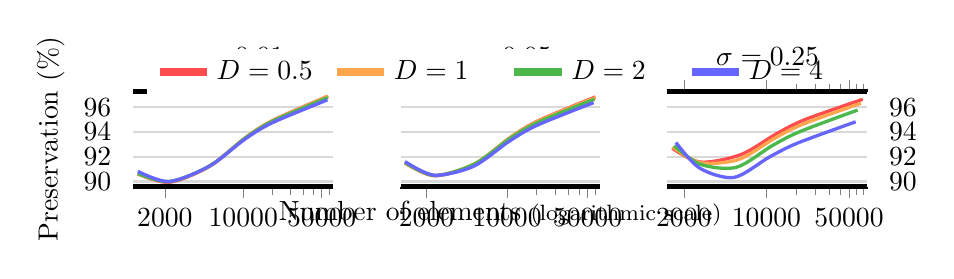
\begin{tikzpicture}
\begin{scope}[shift={(0.0\linewidth,0)}]
\begin{axis}[
 width=0.34\linewidth,height=0.23\linewidth,
 title=\normalsize\mbox{$\sigma=0.01$},
 xmode=log,enlarge x limits=0.025,
 ylabel=Preservation (\%),
 axis y line*=left,
 ymin=89.5852833333,ymax=97.2597858333,
 tick align=outside,
 x axis line style = ultra thick,y axis line style={white},
 xtick={2000,10000,50000},xticklabels={2000,10000,50000},
 minor xtick={18000,26000,34000,42000,58000,66000}, every y tick/.style={white},ymajorgrids,grid style={gray!30,thick}]
\addplot[very thick,mark=none,smooth,color=red!70] table[] {
	1142.66433333 90.6223333333
	2190.331 89.9333333333
	5024.068 91.2336666667
	10557.4073333 93.559
	18518.477 94.946
	57160.1013333 96.8943333333
};
\addplot[very thick,mark=none,smooth,color=orange!70] table[] {
	1142.66433333 90.6223333333
	2203.91966667 89.983
	5019.90933333 91.2416666667
	10559.26 93.5726666667
	18496.2383333 94.9303333333
	56994.2803333 96.8676666667
};
\addplot[very thick,mark=none,smooth,color=green!60!black!70] table[] {
	1147.421 90.6463333333
	2198.01033333 89.9903333333
	5048.57 91.277
	10575.013 93.5463333333
	18463.3696667 94.888
	56796.2563333 96.7726666667
};
\addplot[very thick,mark=none,smooth,color=blue!60!] table[] {
	1148.51366667 90.8193333333
	2179.72533333 89.9976666667
	4988.35566667 91.237
	10445.26 93.4446666667
	18253.313 94.7536666667
	56234.555 96.5863333333
};
!\end{axis}
\end{scope}
\begin{scope}[shift={(0.28\linewidth,0)}]
\begin{axis}[
 width=0.34\linewidth,height=0.23\linewidth,
 title=\normalsize\mbox{$\sigma=0.05$},
 xmode=log,enlarge x limits=0.025,
 xlabel=Number of elements \footnotesize(logarithmic scale),x label style={at={(axis description cs:0.5,-0.05)},anchor=north},
 yticklabels={},
 legend style={at={(0.55,1.45)},legend style={text width=4em},legend style={draw=none},anchor=north,legend columns=-1},
 axis y line*=left,
 ymin=89.5852833333,ymax=97.2597858333,
 tick align=outside,
 x axis line style = ultra thick,y axis line style={white},
 xtick={2000,10000,50000},xticklabels={2000,10000,50000},
 minor xtick={18000,26000,34000,42000,58000,66000}, every y tick/.style={white},ymajorgrids,grid style={gray!30,thick}]
\addlegendimage{line width=3pt,mark=none,red!70}
\addlegendentry{$D=0.5$}
\addlegendimage{line width=3pt,mark=none,orange!70}
\addlegendentry{$D=1$}
\addlegendimage{line width=3pt,mark=none,green!60!black!70}
\addlegendentry{$D=2$}
\addlegendimage{line width=3pt,mark=none,blue!60!}
\addlegendentry{$D=4$}
\addplot[very thick,mark=none,smooth,color=red!70] table[] {
	1298.20533333 91.495
	2340.633 90.4603333333
	5186.95033333 91.389
	10853.1023333 93.6036666667
	18943.9993333 94.9333333333
	58604.5323333 96.8286666667
};
\addplot[very thick,mark=none,smooth,color=orange!70] table[] {
	1297.63266667 91.496
	2349.96633333 90.4843333333
	5211.535 91.4193333333
	10822.068 93.583
	18923.0946667 94.8986666667
	58453.4236667 96.7666666667
};
\addplot[very thick,mark=none,smooth,color=green!60!black!70] table[] {
	1302.89433333 91.533
	2349.60333333 90.4793333333
	5219.07066667 91.411
	10751.7493333 93.5096666667
	18721.5463333 94.7916666667
	57464.189 96.6476666667
};
\addplot[very thick,mark=none,smooth,color=blue!60!] table[] {
	1299.731 91.6113333333
	2327.66833333 90.506
	5087.395 91.215
	10536.52 93.2713333333
	18361.0733333 94.5533333333
	56479.5 96.3676666667
};
!\end{axis}
\end{scope}
\begin{scope}[shift={(0.56\linewidth,0)}]
\begin{axis}[
 width=0.34\linewidth,height=0.23\linewidth,
 title=\normalsize\mbox{$\sigma=0.25$},
 xmode=log,enlarge x limits=0.025,
 axis y line*=right,
 ymin=89.5852833333,ymax=97.2597858333,
 tick align=outside,
 x axis line style = ultra thick,y axis line style={white},
 xtick={2000,10000,50000},xticklabels={2000,10000,50000},
 minor xtick={18000,26000,34000,42000,58000,66000}, every y tick/.style={white},ymajorgrids,grid style={gray!30,thick}]
\addplot[very thick,mark=none,smooth,color=red!70] table[] {
	1596.30333333 92.689
	2756.53766667 91.5646666667
	6060.21733333 92.1663333333
	12338.161 93.8876666667
	21383.8163333 95.011
	65427.1206667 96.6373333333
};
\addplot[very thick,mark=none,smooth,color=orange!70] table[] {
	1607.67666667 92.7946666667
	2757.58366667 91.5123333333
	5836.15333333 91.7793333333
	11813.4666667 93.507
	20455.343 94.6356666667
	63005.4993333 96.319
};
\addplot[very thick,mark=none,smooth,color=green!60!black!70] table[] {
	1656.74966667 92.8756666667
	2746.29366667 91.396
	5559.30066667 91.1436666667
	11210.0 92.8956666667
	19330.474 94.0383333333
	59102.68 95.7656666667
};
\addplot[very thick,mark=none,smooth,color=blue!60!] table[] {
	1714.92766667 93.146
	2716.32133333 91.086
	5316.24133333 90.3253333333
	10718.991 92.003
	18519.036 93.117
	56886.458 94.8183333333
};
!\end{axis}
\end{scope}
\end{tikzpicture}
\end{center}
\caption{Element preservation results using mesh remodelling - RAE 2822 airfoil}\centering\sffamily\footnotesize
Average of thirty optimisation scenarios\end{figure}

\begin{figure}[!h]
\begin{center}
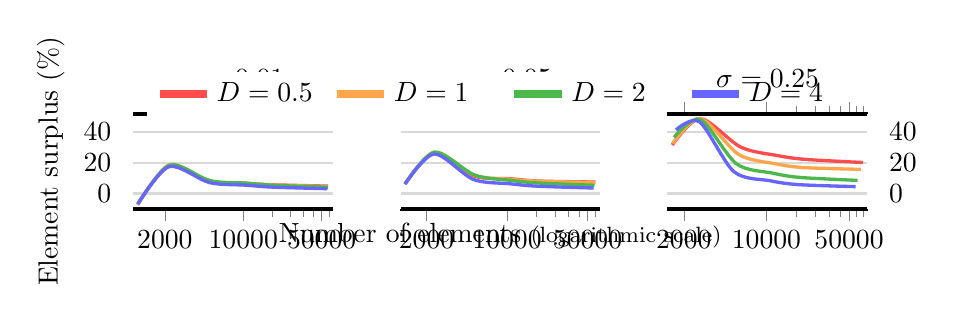
\begin{tikzpicture}
\begin{scope}[shift={(0.0\linewidth,0)}]
\begin{axis}[
 width=0.34\linewidth,height=0.23\linewidth,
 title=\normalsize\mbox{$\sigma=0.01$},
 xmode=log,enlarge x limits=0.025,
 ylabel=Element surplus (\%),
 axis y line*=left,
 ymin=-9.99254435348,ymax=51.7132290624,
 tick align=outside,
 x axis line style = ultra thick,y axis line style={white},
 xtick={2000,10000,50000},xticklabels={2000,10000,50000},
 minor xtick={18000,26000,34000,42000,58000,66000}, every y tick/.style={white},ymajorgrids,grid style={gray!30,thick}]
\addplot[very thick,mark=none,smooth,color=red!70] table[] {
	1142.66433333 -7.19409657952
	2190.331 18.0292948627
	5024.068 7.89971733263
	10557.4073333 6.5949868196
	18518.477 5.68929699423
	57160.1013333 4.84824826573
};
\addplot[very thick,mark=none,smooth,color=orange!70] table[] {
	1142.66433333 -7.19409657952
	2203.91966667 18.7615406944
	5019.90933333 7.81040346231
	10559.26 6.61369264127
	18496.2383333 5.56237570118
	56994.2803333 4.54408433022
};
\addplot[very thick,mark=none,smooth,color=green!60!black!70] table[] {
	1147.421 -6.80776549839
	2198.01033333 18.4431073405
	5048.57 8.42593610078
	10575.013 6.77274597457
	18463.3696667 5.37478650186
	56796.2563333 4.18085072793
};
\addplot[very thick,mark=none,smooth,color=blue!60!] table[] {
	1148.51366667 -6.71902034885
	2179.72533333 17.4577924924
	4988.35566667 7.13273912454
	10445.26 5.46266870957
	18253.313 4.17594377689
	56234.555 3.15052713727
};
!\end{axis}
\end{scope}
\begin{scope}[shift={(0.28\linewidth,0)}]
\begin{axis}[
 width=0.34\linewidth,height=0.23\linewidth,
 title=\normalsize\mbox{$\sigma=0.05$},
 xmode=log,enlarge x limits=0.025,
 xlabel=Number of elements \footnotesize(logarithmic scale),x label style={at={(axis description cs:0.5,-0.05)},anchor=north},
 yticklabels={},
 legend style={at={(0.55,1.45)},legend style={text width=4em},legend style={draw=none},anchor=north,legend columns=-1},
 axis y line*=left,
 ymin=-9.99254435348,ymax=51.7132290624,
 tick align=outside,
 x axis line style = ultra thick,y axis line style={white},
 xtick={2000,10000,50000},xticklabels={2000,10000,50000},
 minor xtick={18000,26000,34000,42000,58000,66000}, every y tick/.style={white},ymajorgrids,grid style={gray!30,thick}]
\addlegendimage{line width=3pt,mark=none,red!70}
\addlegendentry{$D=0.5$}
\addlegendimage{line width=3pt,mark=none,orange!70}
\addlegendentry{$D=1$}
\addlegendimage{line width=3pt,mark=none,green!60!black!70}
\addlegendentry{$D=2$}
\addlegendimage{line width=3pt,mark=none,blue!60!}
\addlegendentry{$D=4$}
\addplot[very thick,mark=none,smooth,color=red!70] table[] {
	1298.20533333 6.06322045678
	2340.633 26.4079832236
	5186.95033333 11.3377964278
	10853.1023333 9.57867583198
	18943.9993333 8.11295780414
	58604.5323333 7.50044176941
};
\addplot[very thick,mark=none,smooth,color=orange!70] table[] {
	1297.63266667 6.01643365861
	2349.96633333 26.9120382563
	5211.535 11.8655058595
	10822.068 9.26533674722
	18923.0946667 7.99365536406
	58453.4236667 7.22325760336
};
\addplot[very thick,mark=none,smooth,color=green!60!black!70] table[] {
	1302.89433333 6.44631119593
	2349.60333333 26.892434116
	5219.07066667 12.0272588102
	10751.7493333 8.55536220326
	18721.5463333 6.84342377496
	57464.189 5.40866819455
};
\addplot[very thick,mark=none,smooth,color=blue!60!] table[] {
	1299.731 6.18786724096
	2327.66833333 25.7078147792
	5087.395 9.20084297278
	10536.52 6.3822927322
	18361.0733333 4.78621285805
	56479.5 3.60241706872
};
!\end{axis}
\end{scope}
\begin{scope}[shift={(0.56\linewidth,0)}]
\begin{axis}[
 width=0.34\linewidth,height=0.23\linewidth,
 title=\normalsize\mbox{$\sigma=0.25$},
 xmode=log,enlarge x limits=0.025,
 axis y line*=right,
 ymin=-9.99254435348,ymax=51.7132290624,
 tick align=outside,
 x axis line style = ultra thick,y axis line style={white},
 xtick={2000,10000,50000},xticklabels={2000,10000,50000},
 minor xtick={18000,26000,34000,42000,58000,66000}, every y tick/.style={white},ymajorgrids,grid style={gray!30,thick}]
\addplot[very thick,mark=none,smooth,color=red!70] table[] {
	1596.30333333 31.5342999505
	2756.53766667 48.7184259783
	6060.21733333 30.1597822272
	12338.161 24.6954469507
	21383.8163333 22.1880437805
	65427.1206667 20.1757517151
};
\addplot[very thick,mark=none,smooth,color=orange!70] table[] {
	1607.67666667 32.4714548176
	2757.58366667 48.7748588997
	5836.15333333 25.3473935221
	11813.4666667 19.3926312064
	20455.343 16.8827073272
	63005.4993333 15.7277466503
};
\addplot[very thick,mark=none,smooth,color=green!60!black!70] table[] {
	1656.74966667 36.5150363642
	2746.29366667 48.1657502162
	5559.30066667 19.4012234724
	11210.0 13.2937040064
	19330.474 10.4551576103
	59102.68 8.55909483723
};
\addplot[very thick,mark=none,smooth,color=blue!60!] table[] {
	1714.92766667 41.3088636668
	2716.32133333 46.5487078336
	5316.24133333 14.1808579055
	10718.991 8.33132859961
	18519.036 5.81856607198
	56886.458 4.48836480809
};
!\end{axis}
\end{scope}
\end{tikzpicture}
\end{center}
\caption{Element surplus results on meshes from mesh remodelling - RAE 2822 airfoil}\centering\sffamily\footnotesize
Average of thirty optimisation scenarios\end{figure}

\input{figures/plots/rae2822_su}
\pagebreak
\subsubsection{NACA 63206}
\vspace*{\fill} \begin{table}[!hp]
\begin{center}
\begin{tabular}{c|cc?c|c?c?c|c|c||c|c}
\multirow{2}{*}{\textbf{\large $\boldsymbol{\sigma}$}} & \multirow{2}{*}{\textbf{\large $\boldsymbol{I}$}} & \multirow{2}{*}{\textbf{\large $\boldsymbol{G}$}} & \multicolumn{2}{c?}{\textbf{\large Generation}} & \multirow{2}{*}{\textbf{\large $\boldsymbol{D}$}} & \multicolumn{5}{c}{\textbf{{\large Remodelling} }} \\\cline{4-5}\cline{7-11}
 & & & \textbf{\# Tri.} & \textbf{Time} & &\textbf{\# Tri.} & \textbf{Time} & \textbf{Preserv.} & \textbf{+ Tri.} & \textbf{Sp.-up} \\\toprule
\multirow{24}[11]{*}{.01} & \multirow{4}{*}{50} & \multirow{4}{*}{1} & \multirow{4}{*}{1218} & \multirow{4}{*}{1.89 ms} & .5 & 1340 & 0.05 ms & 91.71 \% & 10.01 \% & 34.31 \\\cline{6-11}
 & & & &  & 1 & 1340 & 0.06 ms & 91.71 \% & 10.01 \% & 34.25 \\\cline{6-11}
 & & & &  & 2 & 1353 & 0.05 ms & 91.77 \% & 11.12 \% & 34.46 \\\cline{6-11}
 & & & &  & 4 & 1350 & 0.05 ms & 91.81 \% & 10.89 \% & 34.35 \\\cmidrule[1.5pt]{2-11}
 & \multirow{4}{*}{100} & \multirow{4}{*}{2} & \multirow{4}{*}{1913} & \multirow{4}{*}{3.53 ms} & .5 & 2421 & 0.14 ms & 90.63 \% & 26.54 \% & 26.01 \\\cline{6-11}
 & & & &  & 1 & 2437 & 0.14 ms & 90.68 \% & 27.39 \% & 25.98 \\\cline{6-11}
 & & & &  & 2 & 2476 & 0.14 ms & 90.84 \% & 29.42 \% & 25.97 \\\cline{6-11}
 & & & &  & 4 & 2465 & 0.14 ms & 90.86 \% & 28.85 \% & 25.64 \\\cmidrule[1.5pt]{2-11}
 & \multirow{4}{*}{200} & \multirow{4}{*}{4} & \multirow{4}{*}{4824} & \multirow{4}{*}{9.46 ms} & .5 & 5621 & 0.34 ms & 91.96 \% & 16.52 \% & 28.13 \\\cline{6-11}
 & & & &  & 1 & 5562 & 0.34 ms & 91.87 \% & 15.31 \% & 28.06 \\\cline{6-11}
 & & & &  & 2 & 5481 & 0.35 ms & 91.70 \% & 13.62 \% & 26.69 \\\cline{6-11}
 & & & &  & 4 & 5298 & 0.37 ms & 91.38 \% & 9.83 \% & 25.46 \\\cmidrule[1.5pt]{2-11}
 & \multirow{4}{*}{300} & \multirow{4}{*}{6} & \multirow{4}{*}{10184} & \multirow{4}{*}{20.50 ms} & .5 & 11779 & 0.65 ms & 94.03 \% & 15.66 \% & 31.56 \\\cline{6-11}
 & & & &  & 1 & 11592 & 0.66 ms & 93.92 \% & 13.83 \% & 31.25 \\\cline{6-11}
 & & & &  & 2 & 11371 & 0.70 ms & 93.72 \% & 11.66 \% & 29.46 \\\cline{6-11}
 & & & &  & 4 & 10943 & 0.77 ms & 93.33 \% & 7.45 \% & 26.49 \\\cmidrule[1.5pt]{2-11}
 & \multirow{4}{*}{400} & \multirow{4}{*}{8} & \multirow{4}{*}{17993} & \multirow{4}{*}{37.82 ms} & .5 & 20727 & 1.06 ms & 95.28 \% & 15.19 \% & 35.70 \\\cline{6-11}
 & & & &  & 1 & 20333 & 1.08 ms & 95.16 \% & 13.00 \% & 34.89 \\\cline{6-11}
 & & & &  & 2 & 19843 & 1.17 ms & 94.94 \% & 10.28 \% & 32.27 \\\cline{6-11}
 & & & &  & 4 & 19079 & 1.39 ms & 94.54 \% & 6.04 \% & 27.26 \\\cmidrule[1.5pt]{2-11}
 & \multirow{4}{*}{700} & \multirow{4}{*}{14} & \multirow{4}{*}{55800} & \multirow{4}{*}{164.74 ms} & .5 & 64357 & 3.31 ms & 97.01 \% & 15.34 \% & 49.70 \\\cline{6-11}
 & & & &  & 1 & 63204 & 3.59 ms & 96.90 \% & 13.27 \% & 45.88 \\\cline{6-11}
 & & & &  & 2 & 60989 & 4.05 ms & 96.68 \% & 9.30 \% & 40.69 \\\cline{6-11}
 & & & &  & 4 & 58687 & 5.10 ms & 96.28 \% & 5.17 \% & 32.28\\\bottomrule
\end{tabular}\end{center}
\caption{Full results of mesh remodelling for $\sigma=0.01$ - NACA 63206 airfoil}\centering\sffamily\footnotesize
Average of thirty optimisation scenarios\end{table}
 \vspace*{\fill}
\begin{table}[!hp]
\begin{center}
\begin{tabular}{c|cc?c|c?c?c|c|c||c|c}
\multirow{2}{*}{\textbf{\large $\boldsymbol{\sigma}$}} & \multirow{2}{*}{\textbf{\large $\boldsymbol{I}$}} & \multirow{2}{*}{\textbf{\large $\boldsymbol{G}$}} & \multicolumn{2}{c?}{\textbf{\large Generation}} & \multirow{2}{*}{\textbf{\large $\boldsymbol{D}$}} & \multicolumn{5}{c}{\textbf{{\large Remodelling} }} \\\cline{4-5}\cline{7-11}
 & & & \textbf{\# Tri.} & \textbf{Time} & &\textbf{\# Tri.} & \textbf{Time} & \textbf{Preserv.} & \textbf{+ Tri.} & \textbf{Sp.-up} \\\toprule
\multirow{24}[13]{*}{.05} & \multirow{4}{*}{50} & \multirow{4}{*}{1} & \multirow{4}{*}{1234} & \multirow{4}{*}{1.90 ms} & .5 & 1443 & 0.06 ms & 92.05 \% & 16.93 \% & 32.73 \\\cline{6-11}
 & & & &  & 1 & 1444 & 0.06 ms & 92.07 \% & 17.01 \% & 32.94 \\\cline{6-11}
 & & & &  & 2 & 1453 & 0.06 ms & 92.17 \% & 17.72 \% & 33.38 \\\cline{6-11}
 & & & &  & 4 & 1456 & 0.06 ms & 92.20 \% & 18.03 \% & 32.83 \\\cmidrule[1.5pt]{2-11}
 & \multirow{4}{*}{100} & \multirow{4}{*}{2} & \multirow{4}{*}{1918} & \multirow{4}{*}{3.54 ms} & .5 & 2533 & 0.14 ms & 91.00 \% & 32.09 \% & 25.42 \\\cline{6-11}
 & & & &  & 1 & 2542 & 0.14 ms & 90.99 \% & 32.54 \% & 25.11 \\\cline{6-11}
 & & & &  & 2 & 2570 & 0.14 ms & 91.12 \% & 34.01 \% & 25.15 \\\cline{6-11}
 & & & &  & 4 & 2594 & 0.15 ms & 91.20 \% & 35.25 \% & 24.21 \\\cmidrule[1.5pt]{2-11}
 & \multirow{4}{*}{200} & \multirow{4}{*}{4} & \multirow{4}{*}{4825} & \multirow{4}{*}{9.40 ms} & .5 & 5669 & 0.35 ms & 91.98 \% & 17.49 \% & 26.82 \\\cline{6-11}
 & & & &  & 1 & 5601 & 0.36 ms & 91.86 \% & 16.07 \% & 26.46 \\\cline{6-11}
 & & & &  & 2 & 5537 & 0.37 ms & 91.67 \% & 14.74 \% & 25.10 \\\cline{6-11}
 & & & &  & 4 & 5339 & 0.41 ms & 91.27 \% & 10.65 \% & 23.20 \\\cmidrule[1.5pt]{2-11}
 & \multirow{4}{*}{300} & \multirow{4}{*}{6} & \multirow{4}{*}{10189} & \multirow{4}{*}{20.36 ms} & .5 & 11837 & 0.69 ms & 93.98 \% & 16.17 \% & 29.47 \\\cline{6-11}
 & & & &  & 1 & 11628 & 0.70 ms & 93.86 \% & 14.12 \% & 29.25 \\\cline{6-11}
 & & & &  & 2 & 11369 & 0.75 ms & 93.61 \% & 11.58 \% & 27.07 \\\cline{6-11}
 & & & &  & 4 & 10950 & 0.86 ms & 93.19 \% & 7.46 \% & 23.80 \\\cmidrule[1.5pt]{2-11}
 & \multirow{4}{*}{400} & \multirow{4}{*}{8} & \multirow{4}{*}{17999} & \multirow{4}{*}{37.58 ms} & .5 & 20681 & 1.11 ms & 95.22 \% & 14.90 \% & 33.88 \\\cline{6-11}
 & & & &  & 1 & 20296 & 1.17 ms & 95.07 \% & 12.76 \% & 32.16 \\\cline{6-11}
 & & & &  & 2 & 19780 & 1.29 ms & 94.82 \% & 9.90 \% & 29.09 \\\cline{6-11}
 & & & &  & 4 & 19063 & 1.55 ms & 94.39 \% & 5.91 \% & 24.30 \\\cmidrule[1.5pt]{2-11}
 & \multirow{4}{*}{700} & \multirow{4}{*}{14} & \multirow{4}{*}{55826} & \multirow{4}{*}{164.24 ms} & .5 & 63874 & 3.54 ms & 96.94 \% & 14.41 \% & 46.38 \\\cline{6-11}
 & & & &  & 1 & 62901 & 3.91 ms & 96.80 \% & 12.67 \% & 42.01 \\\cline{6-11}
 & & & &  & 2 & 60739 & 4.47 ms & 96.56 \% & 8.80 \% & 36.73 \\\cline{6-11}
 & & & &  & 4 & 58617 & 5.71 ms & 96.11 \% & 5.00 \% & 28.77\\\bottomrule
\end{tabular}\end{center}
\caption{Full results of mesh remodelling for $\sigma=0.05$ - NACA 63206 airfoil}\centering\sffamily\footnotesize
Average of thirty optimisation scenarios\end{table}

\begin{table}[!hp]
\begin{center}
\begin{tabular}{c|cc?c|c?c?c|c|c||c|c}
\multirow{2}{*}{\textbf{\large $\boldsymbol{\sigma}$}} & \multirow{2}{*}{\textbf{\large $\boldsymbol{I}$}} & \multirow{2}{*}{\textbf{\large $\boldsymbol{G}$}} & \multicolumn{2}{c?}{\textbf{\large Generation}} & \multirow{2}{*}{\textbf{\large $\boldsymbol{D}$}} & \multicolumn{5}{c}{\textbf{{\large Remodelling} }} \\\cline{4-5}\cline{7-11}
 & & & \textbf{\# Tri.} & \textbf{Time} & &\textbf{\# Tri.} & \textbf{Time} & \textbf{Preserv.} & \textbf{+ Tri.} & \textbf{Sp.-up} \\\toprule
\multirow{24}[11]{*}{.25} & \multirow{4}{*}{50} & \multirow{4}{*}{1} & \multirow{4}{*}{1234} & \multirow{4}{*}{1.89 ms} & .5 & 1691 & 0.07 ms & 92.97 \% & 37.02 \% & 27.05 \\\cline{6-11}
 & & & &  & 1 & 1677 & 0.07 ms & 92.95 \% & 35.87 \% & 27.28 \\\cline{6-11}
 & & & &  & 2 & 1735 & 0.07 ms & 93.11 \% & 40.57 \% & 26.39 \\\cline{6-11}
 & & & &  & 4 & 1805 & 0.08 ms & 93.32 \% & 46.22 \% & 24.49 \\\cmidrule[1.5pt]{2-11}
 & \multirow{4}{*}{100} & \multirow{4}{*}{2} & \multirow{4}{*}{1923} & \multirow{4}{*}{3.50 ms} & .5 & 2904 & 0.17 ms & 91.89 \% & 51.05 \% & 20.39 \\\cline{6-11}
 & & & &  & 1 & 2901 & 0.17 ms & 91.86 \% & 50.88 \% & 20.12 \\\cline{6-11}
 & & & &  & 2 & 2861 & 0.18 ms & 91.64 \% & 48.78 \% & 19.11 \\\cline{6-11}
 & & & &  & 4 & 2875 & 0.21 ms & 91.45 \% & 49.54 \% & 16.89 \\\cmidrule[1.5pt]{2-11}
 & \multirow{4}{*}{200} & \multirow{4}{*}{4} & \multirow{4}{*}{4815} & \multirow{4}{*}{9.20 ms} & .5 & 6401 & 0.45 ms & 92.54 \% & 32.94 \% & 20.32 \\\cline{6-11}
 & & & &  & 1 & 6100 & 0.46 ms & 92.09 \% & 26.70 \% & 19.88 \\\cline{6-11}
 & & & &  & 2 & 5784 & 0.51 ms & 91.42 \% & 20.12 \% & 17.96 \\\cline{6-11}
 & & & &  & 4 & 5506 & 0.62 ms & 90.53 \% & 14.34 \% & 14.93 \\\cmidrule[1.5pt]{2-11}
 & \multirow{4}{*}{300} & \multirow{4}{*}{6} & \multirow{4}{*}{10166} & \multirow{4}{*}{19.89 ms} & .5 & 13004 & 0.90 ms & 94.19 \% & 27.92 \% & 22.00 \\\cline{6-11}
 & & & &  & 1 & 12252 & 0.96 ms & 93.72 \% & 20.52 \% & 20.72 \\\cline{6-11}
 & & & &  & 2 & 11598 & 1.08 ms & 93.09 \% & 14.09 \% & 18.37 \\\cline{6-11}
 & & & &  & 4 & 11007 & 1.37 ms & 92.13 \% & 8.27 \% & 14.52 \\\cmidrule[1.5pt]{2-11}
 & \multirow{4}{*}{400} & \multirow{4}{*}{8} & \multirow{4}{*}{17955} & \multirow{4}{*}{36.72 ms} & .5 & 22482 & 1.49 ms & 95.24 \% & 25.21 \% & 24.63 \\\cline{6-11}
 & & & &  & 1 & 21241 & 1.64 ms & 94.83 \% & 18.30 \% & 22.45 \\\cline{6-11}
 & & & &  & 2 & 20042 & 1.94 ms & 94.19 \% & 11.62 \% & 18.89 \\\cline{6-11}
 & & & &  & 4 & 19061 & 2.59 ms & 93.25 \% & 6.16 \% & 14.20 \\\cmidrule[1.5pt]{2-11}
 & \multirow{4}{*}{700} & \multirow{4}{*}{14} & \multirow{4}{*}{55701} & \multirow{4}{*}{160.93 ms} & .5 & 68776 & 5.16 ms & 96.78 \% & 23.47 \% & 31.19 \\\cline{6-11}
 & & & &  & 1 & 65460 & 5.98 ms & 96.44 \% & 17.52 \% & 26.92 \\\cline{6-11}
 & & & &  & 2 & 61283 & 7.33 ms & 95.86 \% & 10.02 \% & 21.94 \\\cline{6-11}
 & & & &  & 4 & 58546 & 10.33 ms & 94.91 \% & 5.11 \% & 15.58\\\bottomrule
\end{tabular}\end{center}
\caption{Full results of mesh remodelling for $\sigma=0.25$ - NACA 63206 airfoil}\centering\sffamily\footnotesize
Average of thirty optimisation scenarios\end{table}
 \newpage
\begin{figure}[!h]
\begin{center}
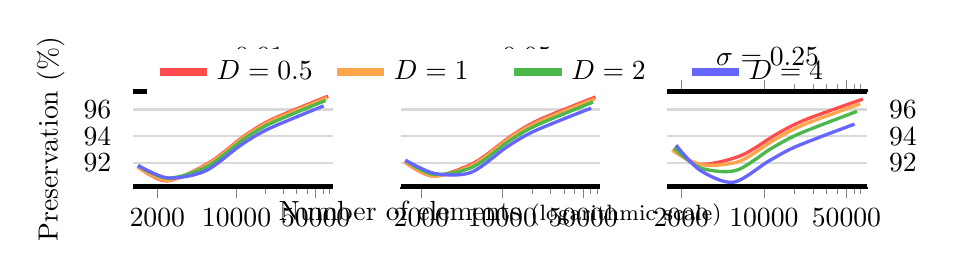
\begin{tikzpicture}
\begin{scope}[shift={(0.0\linewidth,0)}]
\begin{axis}[
 width=0.34\linewidth,height=0.23\linewidth,
 title=\normalsize\mbox{$\sigma=0.01$},
 xmode=log,enlarge x limits=0.025,
 ylabel=Preservation (\%),
 axis y line*=left,
 ymin=90.2097333333,ymax=97.3524633333,
 tick align=outside,
 x axis line style = ultra thick,y axis line style={white},
 xtick={2000,10000,50000},xticklabels={2000,10000,50000},
 minor xtick={18000,26000,34000,42000,58000,66000}, every y tick/.style={white},ymajorgrids,grid style={gray!30,thick}]
\addplot[very thick,mark=none,smooth,color=red!70] table[] {
	1339.73733333 91.7086666667
	2420.84133333 90.6346666667
	5620.72233333 91.9593333333
	11779.2613333 94.029
	20726.7736667 95.2753333333
	64356.625 97.0123333333
};
\addplot[very thick,mark=none,smooth,color=orange!70] table[] {
	1339.73733333 91.7086666667
	2437.06033333 90.6763333333
	5562.499 91.8696666667
	11592.331 93.9196666667
	20332.638 95.1583333333
	63204.0066667 96.8966666667
};
\addplot[very thick,mark=none,smooth,color=green!60!black!70] table[] {
	1353.29366667 91.7726666667
	2475.988 90.8416666667
	5481.227 91.701
	11371.3873333 93.7236666667
	19843.1426667 94.9446666667
	60989.174 96.6806666667
};
\addplot[very thick,mark=none,smooth,color=blue!60!] table[] {
	1350.39633333 91.8063333333
	2464.98566667 90.864
	5298.02166667 91.3796666667
	10942.5643333 93.3313333333
	19078.9953333 94.5446666667
	58686.548 96.2783333333
};
!\end{axis}
\end{scope}
\begin{scope}[shift={(0.28\linewidth,0)}]
\begin{axis}[
 width=0.34\linewidth,height=0.23\linewidth,
 title=\normalsize\mbox{$\sigma=0.05$},
 xmode=log,enlarge x limits=0.025,
 xlabel=Number of elements \footnotesize(logarithmic scale),x label style={at={(axis description cs:0.5,-0.05)},anchor=north},
 yticklabels={},
 legend style={at={(0.55,1.45)},legend style={text width=4em},legend style={draw=none},anchor=north,legend columns=-1},
 axis y line*=left,
 ymin=90.2097333333,ymax=97.3524633333,
 tick align=outside,
 x axis line style = ultra thick,y axis line style={white},
 xtick={2000,10000,50000},xticklabels={2000,10000,50000},
 minor xtick={18000,26000,34000,42000,58000,66000}, every y tick/.style={white},ymajorgrids,grid style={gray!30,thick}]
\addlegendimage{line width=3pt,mark=none,red!70}
\addlegendentry{$D=0.5$}
\addlegendimage{line width=3pt,mark=none,orange!70}
\addlegendentry{$D=1$}
\addlegendimage{line width=3pt,mark=none,green!60!black!70}
\addlegendentry{$D=2$}
\addlegendimage{line width=3pt,mark=none,blue!60!}
\addlegendentry{$D=4$}
\addplot[very thick,mark=none,smooth,color=red!70] table[] {
	1442.82566667 92.0543333333
	2533.24266667 90.9963333333
	5669.485 91.983
	11836.8396667 93.9843333333
	20680.5333333 95.2166666667
	63873.5883333 96.9416666667
};
\addplot[very thick,mark=none,smooth,color=orange!70] table[] {
	1443.78666667 92.0696666667
	2541.81733333 90.9933333333
	5600.65033333 91.8566666667
	11628.1293333 93.8593333333
	20296.073 95.074
	62900.56 96.801
};
\addplot[very thick,mark=none,smooth,color=green!60!black!70] table[] {
	1452.51766667 92.1703333333
	2569.98533333 91.1246666667
	5536.68233333 91.6723333333
	11369.2346667 93.61
	19779.881 94.817
	60739.4833333 96.559
};
\addplot[very thick,mark=none,smooth,color=blue!60!] table[] {
	1456.36 92.2006666667
	2593.726 91.2006666667
	5339.311 91.2663333333
	10949.7836667 93.186
	19062.5516667 94.393
	58616.6363333 96.111
};
!\end{axis}
\end{scope}
\begin{scope}[shift={(0.56\linewidth,0)}]
\begin{axis}[
 width=0.34\linewidth,height=0.23\linewidth,
 title=\normalsize\mbox{$\sigma=0.25$},
 xmode=log,enlarge x limits=0.025,
 axis y line*=right,
 ymin=90.2097333333,ymax=97.3524633333,
 tick align=outside,
 x axis line style = ultra thick,y axis line style={white},
 xtick={2000,10000,50000},xticklabels={2000,10000,50000},
 minor xtick={18000,26000,34000,42000,58000,66000}, every y tick/.style={white},ymajorgrids,grid style={gray!30,thick}]
\addplot[very thick,mark=none,smooth,color=red!70] table[] {
	1691.36433333 92.969
	2904.43666667 91.887
	6401.041 92.5416666667
	13004.1206667 94.1873333333
	22482.168 95.2403333333
	68776.005 96.7843333333
};
\addplot[very thick,mark=none,smooth,color=orange!70] table[] {
	1677.166 92.9476666667
	2901.14533333 91.8643333333
	6100.39133333 92.0893333333
	12251.9936667 93.7186666667
	21241.4256667 94.8286666667
	65459.851 96.4363333333
};
\addplot[very thick,mark=none,smooth,color=green!60!black!70] table[] {
	1735.20633333 93.112
	2860.799 91.636
	5783.71433333 91.421
	11598.037 93.0873333333
	20041.686 94.1946666667
	61282.9063333 95.8633333333
};
\addplot[very thick,mark=none,smooth,color=blue!60!] table[] {
	1804.86366667 93.32
	2875.374 91.4466666667
	5505.542 90.5336666667
	11006.7543333 92.1323333333
	19061.131 93.2513333333
	58545.6053333 94.9093333333
};
!\end{axis}
\end{scope}
\end{tikzpicture}
\end{center}
\caption{Element preservation results using mesh remodelling - NACA 63206 airfoil}\centering\sffamily\footnotesize
Average of thirty optimisation scenarios\end{figure}

\begin{figure}[!h]
\begin{center}
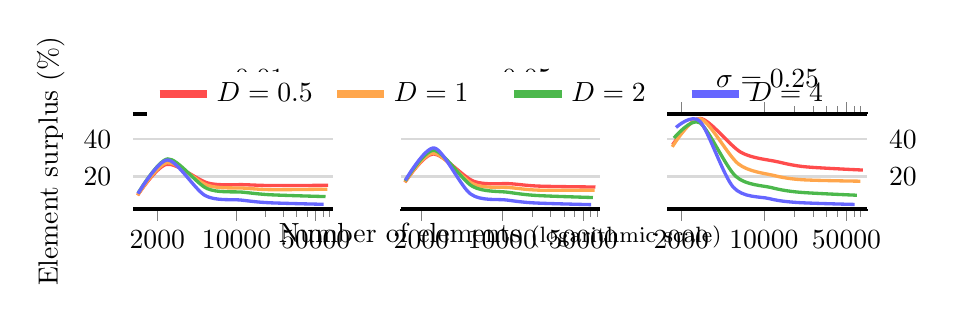
\begin{tikzpicture}
\begin{scope}[shift={(0.0\linewidth,0)}]
\begin{axis}[
 width=0.34\linewidth,height=0.23\linewidth,
 title=\normalsize\mbox{$\sigma=0.01$},
 xmode=log,enlarge x limits=0.025,
 ylabel=Element surplus (\%),
 axis y line*=left,
 ymin=2.69563655211,ymax=53.4657626752,
 tick align=outside,
 x axis line style = ultra thick,y axis line style={white},
 xtick={2000,10000,50000},xticklabels={2000,10000,50000},
 minor xtick={18000,26000,34000,42000,58000,66000}, every y tick/.style={white},ymajorgrids,grid style={gray!30,thick}]
\addplot[very thick,mark=none,smooth,color=red!70] table[] {
	1339.73733333 10.0115945393
	2420.84133333 26.5423126474
	5620.72233333 16.5157546231
	11779.2613333 15.6630938473
	20726.7736667 15.1934227081
	64356.625 15.3350590174
};
\addplot[very thick,mark=none,smooth,color=orange!70] table[] {
	1339.73733333 10.0115945393
	2437.06033333 27.3901128484
	5562.499 15.3088037692
	11592.331 13.8275848051
	20332.638 13.0029304885
	63204.0066667 13.2694239177
};
\addplot[very thick,mark=none,smooth,color=green!60!black!70] table[] {
	1353.29366667 11.124763374
	2475.988 29.4249413595
	5481.227 13.6240615157
	11371.3873333 11.6580915466
	19843.1426667 10.2824567788
	60989.174 9.3001689059
};
\addplot[very thick,mark=none,smooth,color=blue!60!] table[] {
	1350.39633333 10.8868508728
	2464.98566667 28.8498269621
	5298.02166667 9.82627425666
	10942.5643333 7.44738652114
	19078.9953333 6.03554656524
	58686.548 5.17357734513
};
!\end{axis}
\end{scope}
\begin{scope}[shift={(0.28\linewidth,0)}]
\begin{axis}[
 width=0.34\linewidth,height=0.23\linewidth,
 title=\normalsize\mbox{$\sigma=0.05$},
 xmode=log,enlarge x limits=0.025,
 xlabel=Number of elements \footnotesize(logarithmic scale),x label style={at={(axis description cs:0.5,-0.05)},anchor=north},
 yticklabels={},
 legend style={at={(0.55,1.45)},legend style={text width=4em},legend style={draw=none},anchor=north,legend columns=-1},
 axis y line*=left,
 ymin=2.69563655211,ymax=53.4657626752,
 tick align=outside,
 x axis line style = ultra thick,y axis line style={white},
 xtick={2000,10000,50000},xticklabels={2000,10000,50000},
 minor xtick={18000,26000,34000,42000,58000,66000}, every y tick/.style={white},ymajorgrids,grid style={gray!30,thick}]
\addlegendimage{line width=3pt,mark=none,red!70}
\addlegendentry{$D=0.5$}
\addlegendimage{line width=3pt,mark=none,orange!70}
\addlegendentry{$D=1$}
\addlegendimage{line width=3pt,mark=none,green!60!black!70}
\addlegendentry{$D=2$}
\addlegendimage{line width=3pt,mark=none,blue!60!}
\addlegendentry{$D=4$}
\addplot[very thick,mark=none,smooth,color=red!70] table[] {
	1442.82566667 16.9301492289
	2533.24266667 32.0927985122
	5669.485 17.4920768538
	11836.8396667 16.1708317658
	20680.5333333 14.9003842693
	63873.5883333 14.4147493386
};
\addplot[very thick,mark=none,smooth,color=orange!70] table[] {
	1443.78666667 17.0080310382
	2541.81733333 32.5399138759
	5600.65033333 16.0655755144
	11628.1293333 14.1224764865
	20296.073 12.7643349071
	62900.56 12.6717942963
};
\addplot[very thick,mark=none,smooth,color=green!60!black!70] table[] {
	1452.51766667 17.715612804
	2569.98533333 34.0086993174
	5536.68233333 14.7399289747
	11369.2346667 11.5815948311
	19779.881 9.89638860219
	60739.4833333 8.80072565005
};
\addplot[very thick,mark=none,smooth,color=blue!60!] table[] {
	1456.36 18.0270049703
	2593.726 35.2466269505
	5339.311 10.6496865868
	10949.7836667 7.4649578801
	19062.5516667 5.910929682
	58616.6363333 4.99813660305
};
!\end{axis}
\end{scope}
\begin{scope}[shift={(0.56\linewidth,0)}]
\begin{axis}[
 width=0.34\linewidth,height=0.23\linewidth,
 title=\normalsize\mbox{$\sigma=0.25$},
 xmode=log,enlarge x limits=0.025,
 axis y line*=right,
 ymin=2.69563655211,ymax=53.4657626752,
 tick align=outside,
 x axis line style = ultra thick,y axis line style={white},
 xtick={2000,10000,50000},xticklabels={2000,10000,50000},
 minor xtick={18000,26000,34000,42000,58000,66000}, every y tick/.style={white},ymajorgrids,grid style={gray!30,thick}]
\addplot[very thick,mark=none,smooth,color=red!70] table[] {
	1691.36433333 37.0212546477
	2904.43666667 51.0481376217
	6401.041 32.9434040507
	13004.1206667 27.9211229909
	22482.168 25.210606989
	68776.005 23.473751043
};
\addplot[very thick,mark=none,smooth,color=orange!70] table[] {
	1677.166 35.871015513
	2901.14533333 50.8769685355
	6100.39133333 26.6992025039
	12251.9936667 20.5224735214
	21241.4256667 18.3005038053
	65459.851 17.520250641
};
\addplot[very thick,mark=none,smooth,color=green!60!black!70] table[] {
	1735.20633333 40.5729943456
	2860.799 48.7787170639
	5783.71433333 20.1221288116
	11598.037 14.0895225106
	20041.686 11.6187579927
	61282.9063333 10.0213703863
};
\addplot[very thick,mark=none,smooth,color=blue!60!] table[] {
	1804.86366667 46.2160926543
	2875.374 49.5367045357
	5505.542 14.3447596452
	11006.7543333 8.2730936521
	19061.131 6.15772386394
	58545.6053333 5.10708636816
};
!\end{axis}
\end{scope}
\end{tikzpicture}
\end{center}
\caption{Element surplus results on meshes from mesh remodelling - NACA 63206 airfoil}\centering\sffamily\footnotesize
Average of thirty optimisation scenarios\end{figure}

\begin{figure}[!h]
\begin{center}
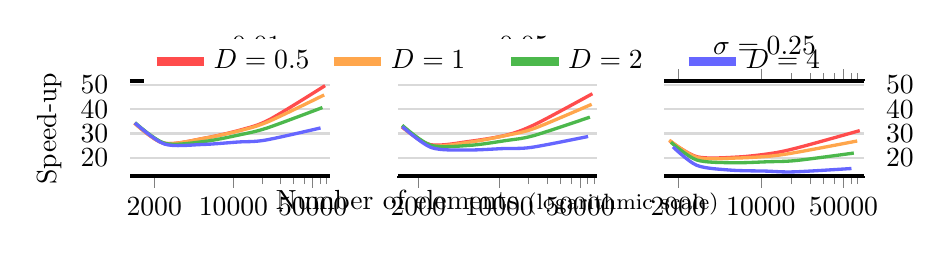
\begin{tikzpicture}
\begin{scope}[shift={(0.0\linewidth,0)}]
\begin{axis}[
 width=0.34\linewidth,height=0.23\linewidth,
 title=\normalsize\mbox{$\sigma=0.01$},
 xmode=log,enlarge x limits=0.025,
 ylabel=Speed-up,
 axis y line*=left,
 ymin=12.4251522816,ymax=51.5637276034,
 tick align=outside,
 x axis line style = ultra thick,y axis line style={white},
 xtick={2000,10000,50000},xticklabels={2000,10000,50000},
 minor xtick={18000,26000,34000,42000,58000,66000}, every y tick/.style={white},ymajorgrids,grid style={gray!30,thick}]
\addplot[very thick,mark=none,smooth,color=red!70] table[] {
	1339.73733333 34.3104912068
	2420.84133333 26.0095823096
	5620.72233333 28.1277017648
	11779.2613333 31.5643828586
	20726.7736667 35.6966932008
	64356.625 49.6999859214
};
\addplot[very thick,mark=none,smooth,color=orange!70] table[] {
	1339.73733333 34.2481840194
	2437.06033333 25.9840451645
	5562.499 28.0581544852
	11592.331 31.2516260163
	20332.638 34.8855543939
	63204.0066667 45.8764132554
};
\addplot[very thick,mark=none,smooth,color=green!60!black!70] table[] {
	1353.29366667 34.4567600487
	2475.988 25.9712953876
	5481.227 26.690751717
	11371.3873333 29.4583772392
	19843.1426667 32.2736530694
	60989.174 40.6851229873
};
\addplot[very thick,mark=none,smooth,color=blue!60!] table[] {
	1350.39633333 34.3521554341
	2464.98566667 25.6441375969
	5298.02166667 25.4641414595
	10942.5643333 26.4860255803
	19078.9953333 27.2636132071
	58686.548 32.2760228571
};
!\end{axis}
\end{scope}
\begin{scope}[shift={(0.28\linewidth,0)}]
\begin{axis}[
 width=0.34\linewidth,height=0.23\linewidth,
 title=\normalsize\mbox{$\sigma=0.05$},
 xmode=log,enlarge x limits=0.025,
 xlabel=Number of elements \footnotesize(logarithmic scale),x label style={at={(axis description cs:0.5,-0.05)},anchor=north},
 yticklabels={},
 legend style={at={(0.55,1.45)},legend style={text width=4em},legend style={draw=none},anchor=north,legend columns=-1},
 axis y line*=left,
 ymin=12.4251522816,ymax=51.5637276034,
 tick align=outside,
 x axis line style = ultra thick,y axis line style={white},
 xtick={2000,10000,50000},xticklabels={2000,10000,50000},
 minor xtick={18000,26000,34000,42000,58000,66000}, every y tick/.style={white},ymajorgrids,grid style={gray!30,thick}]
\addlegendimage{line width=3pt,mark=none,red!70}
\addlegendentry{$D=0.5$}
\addlegendimage{line width=3pt,mark=none,orange!70}
\addlegendentry{$D=1$}
\addlegendimage{line width=3pt,mark=none,green!60!black!70}
\addlegendentry{$D=2$}
\addlegendimage{line width=3pt,mark=none,blue!60!}
\addlegendentry{$D=4$}
\addplot[very thick,mark=none,smooth,color=red!70] table[] {
	1442.82566667 32.7310779817
	2533.24266667 25.4191774271
	5669.485 26.8229473885
	11836.8396667 29.467033232
	20680.5333333 33.8771708431
	63873.5883333 46.3767106526
};
\addplot[very thick,mark=none,smooth,color=orange!70] table[] {
	1443.78666667 32.9388343912
	2541.81733333 25.106991025
	5600.65033333 26.4629247231
	11628.1293333 29.2469720906
	20296.073 32.1646602385
	62900.56 42.0141885094
};
\addplot[very thick,mark=none,smooth,color=green!60!black!70] table[] {
	1452.51766667 33.381871345
	2569.98533333 25.1545196403
	5536.68233333 25.098905012
	11369.2346667 27.0746731664
	19779.881 29.0930202555
	60739.4833333 36.7308996847
};
\addplot[very thick,mark=none,smooth,color=blue!60!] table[] {
	1456.36 32.825186889
	2593.726 24.2092917331
	5339.311 23.2026993663
	10949.7836667 23.8044028833
	19062.5516667 24.2953801069
	58616.6363333 28.7689244656
};
!\end{axis}
\end{scope}
\begin{scope}[shift={(0.56\linewidth,0)}]
\begin{axis}[
 width=0.34\linewidth,height=0.23\linewidth,
 title=\normalsize\mbox{$\sigma=0.25$},
 xmode=log,enlarge x limits=0.025,
 axis y line*=right,
 ymin=12.4251522816,ymax=51.5637276034,
 tick align=outside,
 x axis line style = ultra thick,y axis line style={white},
 xtick={2000,10000,50000},xticklabels={2000,10000,50000},
 minor xtick={18000,26000,34000,42000,58000,66000}, every y tick/.style={white},ymajorgrids,grid style={gray!30,thick}]
\addplot[very thick,mark=none,smooth,color=red!70] table[] {
	1691.36433333 27.0462345091
	2904.43666667 20.3891912908
	6401.041 20.315700412
	13004.1206667 22.0015482729
	22482.168 24.6333959395
	68776.005 31.1853215513
};
\addplot[very thick,mark=none,smooth,color=orange!70] table[] {
	1677.166 27.2802884615
	2901.14533333 20.1193170919
	6100.39133333 19.8755488375
	12251.9936667 20.7241918122
	21241.4256667 22.4516812717
	65459.851 26.9171610169
};
\addplot[very thick,mark=none,smooth,color=green!60!black!70] table[] {
	1735.20633333 26.3920930233
	2860.799 19.1146345909
	5783.71433333 17.9597398374
	11598.037 18.3726643066
	20041.686 18.8864622084
	61282.9063333 21.9434308726
};
\addplot[very thick,mark=none,smooth,color=blue!60!] table[] {
	1804.86366667 24.4898575744
	2875.374 16.8864917083
	5505.542 14.9324572788
	11006.7543333 14.5173185445
	19061.131 14.2001443597
	58545.6053333 15.5812877199
};
!\end{axis}
\end{scope}
\end{tikzpicture}
\end{center}
\caption{Speed-up results by mesh remodelling - NACA 63206 airfoil}\centering\sffamily\footnotesize
Average of thirty optimisation scenarios\end{figure}

\pagebreak
\subsubsection{Eppler 376}
\vspace*{\fill} \begin{table}[!hp]
\begin{center}
\begin{tabular}{c|cc?c|c?c?c|c|c||c|c}
\multirow{2}{*}{\textbf{\large $\boldsymbol{\sigma}$}} & \multirow{2}{*}{\textbf{\large $\boldsymbol{I}$}} & \multirow{2}{*}{\textbf{\large $\boldsymbol{G}$}} & \multicolumn{2}{c?}{\textbf{\large Generation}} & \multirow{2}{*}{\textbf{\large $\boldsymbol{D}$}} & \multicolumn{5}{c}{\textbf{{\large Remodelling} }} \\\cline{4-5}\cline{7-11}
 & & & \textbf{\# Tri.} & \textbf{Time} & &\textbf{\# Tri.} & \textbf{Time} & \textbf{Preserv.} & \textbf{+ Tri.} & \textbf{Sp.-up} \\\toprule
\multirow{24}[13]{*}{.01} & \multirow{4}{*}{50} & \multirow{4}{*}{1} & \multirow{4}{*}{1210} & \multirow{4}{*}{1.78 ms} & .5 & 1598 & 0.07 ms & 92.70 \% & 32.00 \% & 25.53 \\\cline{6-11}
 & & & &  & 1 & 1585 & 0.07 ms & 92.66 \% & 30.99 \% & 25.95 \\\cline{6-11}
 & & & &  & 2 & 1616 & 0.07 ms & 92.77 \% & 33.51 \% & 25.71 \\\cline{6-11}
 & & & &  & 4 & 1614 & 0.07 ms & 92.70 \% & 33.39 \% & 24.76 \\\cmidrule[1.5pt]{2-11}
 & \multirow{4}{*}{100} & \multirow{4}{*}{2} & \multirow{4}{*}{1934} & \multirow{4}{*}{3.27 ms} & .5 & 2740 & 0.17 ms & 91.52 \% & 41.65 \% & 18.78 \\\cline{6-11}
 & & & &  & 1 & 2714 & 0.17 ms & 91.44 \% & 40.30 \% & 18.72 \\\cline{6-11}
 & & & &  & 2 & 2715 & 0.18 ms & 91.42 \% & 40.35 \% & 18.41 \\\cline{6-11}
 & & & &  & 4 & 2738 & 0.19 ms & 91.33 \% & 41.56 \% & 17.38 \\\cmidrule[1.5pt]{2-11}
 & \multirow{4}{*}{200} & \multirow{4}{*}{4} & \multirow{4}{*}{4768} & \multirow{4}{*}{8.41 ms} & .5 & 6220 & 0.48 ms & 92.43 \% & 30.44 \% & 17.58 \\\cline{6-11}
 & & & &  & 1 & 5987 & 0.48 ms & 92.11 \% & 25.55 \% & 17.63 \\\cline{6-11}
 & & & &  & 2 & 5687 & 0.51 ms & 91.54 \% & 19.26 \% & 16.48 \\\cline{6-11}
 & & & &  & 4 & 5399 & 0.58 ms & 90.73 \% & 13.22 \% & 14.58 \\\cmidrule[1.5pt]{2-11}
 & \multirow{4}{*}{300} & \multirow{4}{*}{6} & \multirow{4}{*}{10103} & \multirow{4}{*}{18.17 ms} & .5 & 12841 & 0.97 ms & 94.19 \% & 27.10 \% & 18.68 \\\cline{6-11}
 & & & &  & 1 & 12307 & 1.00 ms & 93.88 \% & 21.82 \% & 18.09 \\\cline{6-11}
 & & & &  & 2 & 11575 & 1.10 ms & 93.29 \% & 14.57 \% & 16.47 \\\cline{6-11}
 & & & &  & 4 & 11013 & 1.31 ms & 92.48 \% & 9.01 \% & 13.91 \\\cmidrule[1.5pt]{2-11}
 & \multirow{4}{*}{400} & \multirow{4}{*}{8} & \multirow{4}{*}{17867} & \multirow{4}{*}{33.71 ms} & .5 & 22453 & 1.62 ms & 95.31 \% & 25.67 \% & 20.76 \\\cline{6-11}
 & & & &  & 1 & 21450 & 1.72 ms & 94.98 \% & 20.05 \% & 19.56 \\\cline{6-11}
 & & & &  & 2 & 20057 & 1.93 ms & 94.42 \% & 12.26 \% & 17.50 \\\cline{6-11}
 & & & &  & 4 & 19064 & 2.45 ms & 93.58 \% & 6.70 \% & 13.78 \\\cmidrule[1.5pt]{2-11}
 & \multirow{4}{*}{700} & \multirow{4}{*}{14} & \multirow{4}{*}{55533} & \multirow{4}{*}{151.14 ms} & .5 & 69114 & 5.52 ms & 96.85 \% & 24.46 \% & 27.37 \\\cline{6-11}
 & & & &  & 1 & 66056 & 6.13 ms & 96.55 \% & 18.95 \% & 24.66 \\\cline{6-11}
 & & & &  & 2 & 61394 & 7.01 ms & 96.06 \% & 10.55 \% & 21.56 \\\cline{6-11}
 & & & &  & 4 & 58530 & 9.56 ms & 95.19 \% & 5.40 \% & 15.82\\\bottomrule
\end{tabular}\end{center}
\caption{Full results of mesh remodelling for $\sigma=0.01$ - Eppler 376 airfoil}\centering\sffamily\footnotesize
Average of thirty optimisation scenarios\end{table}
 \vspace*{\fill}
\begin{table}[!hp]
\begin{center}
\begin{tabular}{c|cc?c|c?c?c|c|c||c|c}
\multirow{2}{*}{\textbf{\large $\boldsymbol{\sigma}$}} & \multirow{2}{*}{\textbf{\large $\boldsymbol{I}$}} & \multirow{2}{*}{\textbf{\large $\boldsymbol{G}$}} & \multicolumn{2}{c?}{\textbf{\large Generation}} & \multirow{2}{*}{\textbf{\large $\boldsymbol{D}$}} & \multicolumn{5}{c}{\textbf{{\large Remodelling} }} \\\cline{4-5}\cline{7-11}
 & & & \textbf{\# Tri.} & \textbf{Time} & &\textbf{\# Tri.} & \textbf{Time} & \textbf{Preserv.} & \textbf{+ Tri.} & \textbf{Sp.-up} \\\toprule
\multirow{24}[11]{*}{.05} & \multirow{4}{*}{50} & \multirow{4}{*}{1} & \multirow{4}{*}{1210} & \multirow{4}{*}{1.77 ms} & .5 & 1608 & 0.07 ms & 92.70 \% & 32.95 \% & 24.47 \\\cline{6-11}
 & & & &  & 1 & 1594 & 0.07 ms & 92.61 \% & 31.80 \% & 24.49 \\\cline{6-11}
 & & & &  & 2 & 1605 & 0.07 ms & 92.63 \% & 32.66 \% & 24.61 \\\cline{6-11}
 & & & &  & 4 & 1647 & 0.07 ms & 92.82 \% & 36.17 \% & 23.77 \\\cmidrule[1.5pt]{2-11}
 & \multirow{4}{*}{100} & \multirow{4}{*}{2} & \multirow{4}{*}{1936} & \multirow{4}{*}{3.27 ms} & .5 & 2816 & 0.18 ms & 91.71 \% & 45.45 \% & 18.20 \\\cline{6-11}
 & & & &  & 1 & 2784 & 0.18 ms & 91.63 \% & 43.83 \% & 18.02 \\\cline{6-11}
 & & & &  & 2 & 2771 & 0.18 ms & 91.55 \% & 43.15 \% & 17.83 \\\cline{6-11}
 & & & &  & 4 & 2748 & 0.20 ms & 91.28 \% & 41.97 \% & 16.31 \\\cmidrule[1.5pt]{2-11}
 & \multirow{4}{*}{200} & \multirow{4}{*}{4} & \multirow{4}{*}{4767} & \multirow{4}{*}{8.37 ms} & .5 & 6255 & 0.49 ms & 92.41 \% & 31.20 \% & 16.99 \\\cline{6-11}
 & & & &  & 1 & 6009 & 0.49 ms & 92.06 \% & 26.04 \% & 16.95 \\\cline{6-11}
 & & & &  & 2 & 5749 & 0.54 ms & 91.52 \% & 20.60 \% & 15.56 \\\cline{6-11}
 & & & &  & 4 & 5426 & 0.61 ms & 90.63 \% & 13.83 \% & 13.79 \\\cmidrule[1.5pt]{2-11}
 & \multirow{4}{*}{300} & \multirow{4}{*}{6} & \multirow{4}{*}{10101} & \multirow{4}{*}{18.10 ms} & .5 & 12940 & 1.01 ms & 94.17 \% & 28.10 \% & 17.90 \\\cline{6-11}
 & & & &  & 1 & 12319 & 1.05 ms & 93.80 \% & 21.95 \% & 17.31 \\\cline{6-11}
 & & & &  & 2 & 11598 & 1.15 ms & 93.19 \% & 14.82 \% & 15.76 \\\cline{6-11}
 & & & &  & 4 & 11030 & 1.38 ms & 92.33 \% & 9.20 \% & 13.11 \\\cmidrule[1.5pt]{2-11}
 & \multirow{4}{*}{400} & \multirow{4}{*}{8} & \multirow{4}{*}{17863} & \multirow{4}{*}{33.60 ms} & .5 & 22515 & 1.67 ms & 95.25 \% & 26.04 \% & 20.14 \\\cline{6-11}
 & & & &  & 1 & 21445 & 1.78 ms & 94.90 \% & 20.05 \% & 18.86 \\\cline{6-11}
 & & & &  & 2 & 20081 & 2.02 ms & 94.31 \% & 12.42 \% & 16.66 \\\cline{6-11}
 & & & &  & 4 & 19092 & 2.60 ms & 93.42 \% & 6.88 \% & 12.93 \\\cmidrule[1.5pt]{2-11}
 & \multirow{4}{*}{700} & \multirow{4}{*}{14} & \multirow{4}{*}{55526} & \multirow{4}{*}{151.14 ms} & .5 & 69029 & 5.74 ms & 96.79 \% & 24.32 \% & 26.34 \\\cline{6-11}
 & & & &  & 1 & 65971 & 6.41 ms & 96.47 \% & 18.81 \% & 23.57 \\\cline{6-11}
 & & & &  & 2 & 61432 & 7.47 ms & 95.94 \% & 10.64 \% & 20.24 \\\cline{6-11}
 & & & &  & 4 & 58570 & 10.22 ms & 95.01 \% & 5.48 \% & 14.79\\\bottomrule
\end{tabular}\end{center}
\caption{Full results of mesh remodelling for $\sigma=0.05$ - Eppler 376 airfoil}\centering\sffamily\footnotesize
Average of thirty optimisation scenarios\end{table}

\begin{table}[!hp]
\begin{center}
\begin{tabular}{c|cc?c|c?c?c|c|c||c|c}
\multirow{2}{*}{\textbf{\large $\boldsymbol{\sigma}$}} & \multirow{2}{*}{\textbf{\large $\boldsymbol{I}$}} & \multirow{2}{*}{\textbf{\large $\boldsymbol{G}$}} & \multicolumn{2}{c?}{\textbf{\large Generation}} & \multirow{2}{*}{\textbf{\large $\boldsymbol{D}$}} & \multicolumn{5}{c}{\textbf{{\large Remodelling} }} \\\cline{4-5}\cline{7-11}
 & & & \textbf{\# Tri.} & \textbf{Time} & &\textbf{\# Tri.} & \textbf{Time} & \textbf{Preserv.} & \textbf{+ Tri.} & \textbf{Sp.-up} \\\toprule
\multirow{24}[13]{*}{.25} & \multirow{4}{*}{50} & \multirow{4}{*}{1} & \multirow{4}{*}{1207} & \multirow{4}{*}{1.77 ms} & .5 & 1730 & 0.08 ms & 93.15 \% & 43.27 \% & 23.10 \\\cline{6-11}
 & & & &  & 1 & 1730 & 0.08 ms & 93.15 \% & 43.31 \% & 22.96 \\\cline{6-11}
 & & & &  & 2 & 1773 & 0.08 ms & 93.24 \% & 46.83 \% & 22.07 \\\cline{6-11}
 & & & &  & 4 & 1825 & 0.09 ms & 93.32 \% & 51.15 \% & 20.51 \\\cmidrule[1.5pt]{2-11}
 & \multirow{4}{*}{100} & \multirow{4}{*}{2} & \multirow{4}{*}{1938} & \multirow{4}{*}{3.25 ms} & .5 & 2962 & 0.19 ms & 92.05 \% & 52.85 \% & 17.55 \\\cline{6-11}
 & & & &  & 1 & 2923 & 0.19 ms & 91.90 \% & 50.82 \% & 17.34 \\\cline{6-11}
 & & & &  & 2 & 2923 & 0.20 ms & 91.78 \% & 50.84 \% & 16.22 \\\cline{6-11}
 & & & &  & 4 & 2863 & 0.23 ms & 91.27 \% & 47.74 \% & 13.87 \\\cmidrule[1.5pt]{2-11}
 & \multirow{4}{*}{200} & \multirow{4}{*}{4} & \multirow{4}{*}{4764} & \multirow{4}{*}{8.34 ms} & .5 & 6693 & 0.52 ms & 92.77 \% & 40.50 \% & 16.11 \\\cline{6-11}
 & & & &  & 1 & 6279 & 0.53 ms & 92.19 \% & 31.81 \% & 15.75 \\\cline{6-11}
 & & & &  & 2 & 5860 & 0.59 ms & 91.38 \% & 23.01 \% & 14.14 \\\cline{6-11}
 & & & &  & 4 & 5562 & 0.71 ms & 90.32 \% & 16.76 \% & 11.76 \\\cmidrule[1.5pt]{2-11}
 & \multirow{4}{*}{300} & \multirow{4}{*}{6} & \multirow{4}{*}{10089} & \multirow{4}{*}{18.02 ms} & .5 & 13606 & 1.07 ms & 94.31 \% & 34.86 \% & 16.90 \\\cline{6-11}
 & & & &  & 1 & 12649 & 1.12 ms & 93.77 \% & 25.38 \% & 16.05 \\\cline{6-11}
 & & & &  & 2 & 11707 & 1.28 ms & 92.95 \% & 16.04 \% & 14.10 \\\cline{6-11}
 & & & &  & 4 & 11066 & 1.61 ms & 91.80 \% & 9.69 \% & 11.21 \\\cmidrule[1.5pt]{2-11}
 & \multirow{4}{*}{400} & \multirow{4}{*}{8} & \multirow{4}{*}{17845} & \multirow{4}{*}{33.46 ms} & .5 & 23499 & 1.77 ms & 95.31 \% & 31.68 \% & 18.87 \\\cline{6-11}
 & & & &  & 1 & 21894 & 1.94 ms & 94.81 \% & 22.69 \% & 17.26 \\\cline{6-11}
 & & & &  & 2 & 20180 & 2.31 ms & 94.03 \% & 13.09 \% & 14.50 \\\cline{6-11}
 & & & &  & 4 & 19062 & 3.09 ms & 92.85 \% & 6.82 \% & 10.83 \\\cmidrule[1.5pt]{2-11}
 & \multirow{4}{*}{700} & \multirow{4}{*}{14} & \multirow{4}{*}{55458} & \multirow{4}{*}{150.16 ms} & .5 & 71718 & 6.26 ms & 96.77 \% & 29.32 \% & 23.98 \\\cline{6-11}
 & & & &  & 1 & 67278 & 7.18 ms & 96.35 \% & 21.31 \% & 20.93 \\\cline{6-11}
 & & & &  & 2 & 61629 & 8.65 ms & 95.64 \% & 11.13 \% & 17.36 \\\cline{6-11}
 & & & &  & 4 & 58557 & 12.39 ms & 94.44 \% & 5.59 \% & 12.12\\\bottomrule
\end{tabular}\end{center}
\caption{Full results of mesh remodelling for $\sigma=0.25$ - Eppler 376 airfoil}\centering\sffamily\footnotesize
Average of thirty optimisation scenarios\end{table}
 \newpage
\begin{figure}[!h]
\begin{center}
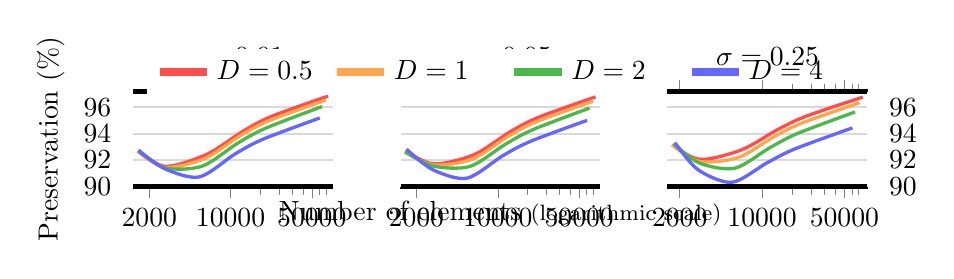
\begin{tikzpicture}
\begin{scope}[shift={(0.0\linewidth,0)}]
\begin{axis}[
 width=0.34\linewidth,height=0.23\linewidth,
 title=\normalsize\mbox{$\sigma=0.01$},
 xmode=log,enlarge x limits=0.025,
 ylabel=Preservation (\%),
 axis y line*=left,
 ymin=89.9891,ymax=97.189895,
 tick align=outside,
 x axis line style = ultra thick,y axis line style={white},
 xtick={2000,10000,50000},xticklabels={2000,10000,50000},
 minor xtick={18000,26000,34000,42000,58000,66000}, every y tick/.style={white},ymajorgrids,grid style={gray!30,thick}]
\addplot[very thick,mark=none,smooth,color=red!70] table[] {
	1597.56966667 92.6966666667
	2740.0 91.5226666667
	6219.95666667 92.427
	12841.0846667 94.191
	22453.2753333 95.3053333333
	69114.4313333 96.847
};
\addplot[very thick,mark=none,smooth,color=orange!70] table[] {
	1585.37333333 92.6606666667
	2713.76166667 91.445
	5986.56433333 92.1116666667
	12307.4733333 93.88
	21449.891 94.9793333333
	66056.1383333 96.5516666667
};
\addplot[very thick,mark=none,smooth,color=green!60!black!70] table[] {
	1615.85633333 92.7716666667
	2714.83633333 91.417
	5686.62733333 91.5383333333
	11574.5646667 93.2903333333
	20057.094 94.4156666667
	61394.3783333 96.057
};
\addplot[very thick,mark=none,smooth,color=blue!60!] table[] {
	1614.35233333 92.7013333333
	2738.08866667 91.332
	5399.01866667 90.7253333333
	11013.093 92.482
	19064.4793333 93.584
	58529.946 95.1883333333
};
!\end{axis}
\end{scope}
\begin{scope}[shift={(0.28\linewidth,0)}]
\begin{axis}[
 width=0.34\linewidth,height=0.23\linewidth,
 title=\normalsize\mbox{$\sigma=0.05$},
 xmode=log,enlarge x limits=0.025,
 xlabel=Number of elements \footnotesize(logarithmic scale),x label style={at={(axis description cs:0.5,-0.05)},anchor=north},
 yticklabels={},
 legend style={at={(0.55,1.45)},legend style={text width=4em},legend style={draw=none},anchor=north,legend columns=-1},
 axis y line*=left,
 ymin=89.9891,ymax=97.189895,
 tick align=outside,
 x axis line style = ultra thick,y axis line style={white},
 xtick={2000,10000,50000},xticklabels={2000,10000,50000},
 minor xtick={18000,26000,34000,42000,58000,66000}, every y tick/.style={white},ymajorgrids,grid style={gray!30,thick}]
\addlegendimage{line width=3pt,mark=none,red!70}
\addlegendentry{$D=0.5$}
\addlegendimage{line width=3pt,mark=none,orange!70}
\addlegendentry{$D=1$}
\addlegendimage{line width=3pt,mark=none,green!60!black!70}
\addlegendentry{$D=2$}
\addlegendimage{line width=3pt,mark=none,blue!60!}
\addlegendentry{$D=4$}
\addplot[very thick,mark=none,smooth,color=red!70] table[] {
	1608.38566667 92.7036666667
	2815.783 91.7103333333
	6254.791 92.4063333333
	12939.9666667 94.1726666667
	22515.0153333 95.248
	69028.7106667 96.7856666667
};
\addplot[very thick,mark=none,smooth,color=orange!70] table[] {
	1594.41933333 92.6116666667
	2784.365 91.634
	6008.57 92.062
	12318.54 93.797
	21444.6516667 94.9023333333
	65971.1733333 96.4693333333
};
\addplot[very thick,mark=none,smooth,color=green!60!black!70] table[] {
	1604.80333333 92.6296666667
	2771.266 91.5523333333
	5749.36966667 91.5163333333
	11597.869 93.193
	20081.009 94.3106666667
	61432.4436667 95.94
};
\addplot[very thick,mark=none,smooth,color=blue!60!] table[] {
	1647.27933333 92.823
	2748.387 91.2833333333
	5426.47433333 90.6263333333
	11030.181 92.3283333333
	19092.137 93.4203333333
	58569.6863333 95.0116666667
};
!\end{axis}
\end{scope}
\begin{scope}[shift={(0.56\linewidth,0)}]
\begin{axis}[
 width=0.34\linewidth,height=0.23\linewidth,
 title=\normalsize\mbox{$\sigma=0.25$},
 xmode=log,enlarge x limits=0.025,
 axis y line*=right,
 ymin=89.9891,ymax=97.189895,
 tick align=outside,
 x axis line style = ultra thick,y axis line style={white},
 xtick={2000,10000,50000},xticklabels={2000,10000,50000},
 minor xtick={18000,26000,34000,42000,58000,66000}, every y tick/.style={white},ymajorgrids,grid style={gray!30,thick}]
\addplot[very thick,mark=none,smooth,color=red!70] table[] {
	1729.68166667 93.151
	2962.25533333 92.0506666667
	6692.924 92.771
	13605.839 94.3123333333
	23499.072 95.31
	71717.803 96.7676666667
};
\addplot[very thick,mark=none,smooth,color=orange!70] table[] {
	1730.17 93.152
	2922.996 91.9006666667
	6278.947 92.192
	12649.4086667 93.773
	21893.7756667 94.8106666667
	67277.523 96.3466666667
};
\addplot[very thick,mark=none,smooth,color=green!60!black!70] table[] {
	1772.74233333 93.2436666667
	2923.30333333 91.7846666667
	5859.619 91.3836666667
	11707.061 92.9486666667
	20179.976 94.029
	61628.7326667 95.643
};
\addplot[very thick,mark=none,smooth,color=blue!60!] table[] {
	1824.84966667 93.317
	2863.199 91.269
	5561.88933333 90.3156666667
	11065.8646667 91.8006666667
	19061.8436667 92.8496666667
	58557.4696667 94.4393333333
};
!\end{axis}
\end{scope}
\end{tikzpicture}
\end{center}
\caption{Element preservation results using mesh remodelling - Eppler 376 airfoil}\centering\sffamily\footnotesize
Average of thirty optimisation scenarios\end{figure}

\begin{figure}[!h]
\begin{center}
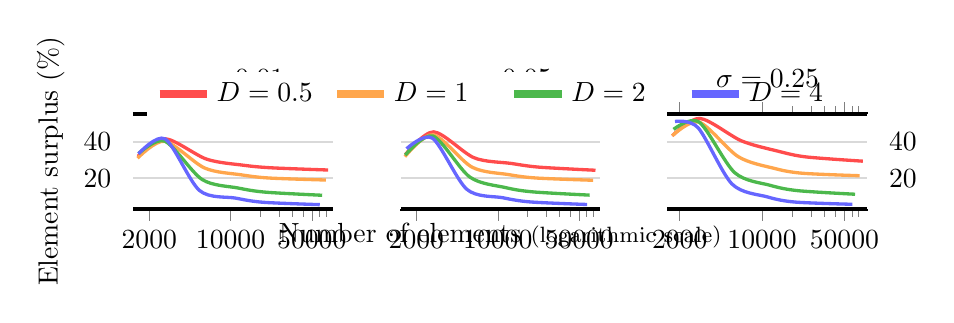
\begin{tikzpicture}
\begin{scope}[shift={(0.0\linewidth,0)}]
\begin{axis}[
 width=0.34\linewidth,height=0.23\linewidth,
 title=\normalsize\mbox{$\sigma=0.01$},
 xmode=log,enlarge x limits=0.025,
 ylabel=Element surplus (\%),
 axis y line*=left,
 ymin=3.02435880427,ymax=55.3384618855,
 tick align=outside,
 x axis line style = ultra thick,y axis line style={white},
 xtick={2000,10000,50000},xticklabels={2000,10000,50000},
 minor xtick={18000,26000,34000,42000,58000,66000}, every y tick/.style={white},ymajorgrids,grid style={gray!30,thick}]
\addplot[very thick,mark=none,smooth,color=red!70] table[] {
	1597.56966667 31.9986240243
	2740.0 41.6548979938
	6219.95666667 30.4411864834
	12841.0846667 27.1014265864
	22453.2753333 25.6667617441
	69114.4313333 24.4567261192
};
\addplot[very thick,mark=none,smooth,color=orange!70] table[] {
	1585.37333333 30.9909063317
	2713.76166667 40.2984058654
	5986.56433333 25.5466229828
	12307.4733333 21.8197262106
	21449.891 20.0510082256
	66056.1383333 18.9495530593
};
\addplot[very thick,mark=none,smooth,color=green!60!black!70] table[] {
	1615.85633333 33.5095533367
	2714.83633333 40.3539649154
	5686.62733333 19.2565247961
	11574.5646667 14.5653750784
	20057.094 12.2557852054
	61394.3783333 10.5549619969
};
\addplot[very thick,mark=none,smooth,color=blue!60!] table[] {
	1614.35233333 33.385285873
	2738.08866667 41.5560842243
	5399.01866667 13.2249689938
	11013.093 9.0079123193
	19064.4793333 6.70030748699
	58529.946 5.39688048596
};
!\end{axis}
\end{scope}
\begin{scope}[shift={(0.28\linewidth,0)}]
\begin{axis}[
 width=0.34\linewidth,height=0.23\linewidth,
 title=\normalsize\mbox{$\sigma=0.05$},
 xmode=log,enlarge x limits=0.025,
 xlabel=Number of elements \footnotesize(logarithmic scale),x label style={at={(axis description cs:0.5,-0.05)},anchor=north},
 yticklabels={},
 legend style={at={(0.55,1.45)},legend style={text width=4em},legend style={draw=none},anchor=north,legend columns=-1},
 axis y line*=left,
 ymin=3.02435880427,ymax=55.3384618855,
 tick align=outside,
 x axis line style = ultra thick,y axis line style={white},
 xtick={2000,10000,50000},xticklabels={2000,10000,50000},
 minor xtick={18000,26000,34000,42000,58000,66000}, every y tick/.style={white},ymajorgrids,grid style={gray!30,thick}]
\addlegendimage{line width=3pt,mark=none,red!70}
\addlegendentry{$D=0.5$}
\addlegendimage{line width=3pt,mark=none,orange!70}
\addlegendentry{$D=1$}
\addlegendimage{line width=3pt,mark=none,green!60!black!70}
\addlegendentry{$D=2$}
\addlegendimage{line width=3pt,mark=none,blue!60!}
\addlegendentry{$D=4$}
\addplot[very thick,mark=none,smooth,color=red!70] table[] {
	1608.38566667 32.9528205058
	2815.783 45.4530787272
	6254.791 31.2000785898
	12939.9666667 28.103553345
	22515.0153333 26.0419465148
	69028.7106667 24.3168789276
};
\addplot[very thick,mark=none,smooth,color=orange!70] table[] {
	1594.41933333 31.7983315997
	2784.365 43.8301394498
	6008.57 26.0353633259
	12318.54 21.9515309949
	21444.6516667 20.0499132859
	65971.1733333 18.8104237901
};
\addplot[very thick,mark=none,smooth,color=green!60!black!70] table[] {
	1604.80333333 32.6566966777
	2771.266 43.1534928906
	5749.36966667 20.5983944321
	11597.869 14.8170059786
	20081.009 12.4160665613
	61432.4436667 10.6364234212
};
\addplot[very thick,mark=none,smooth,color=blue!60!] table[] {
	1647.27933333 36.1678595292
	2748.387 41.9716472057
	5426.47433333 13.8253634692
	11030.181 9.19698763817
	19092.137 6.88023414508
	58569.6863333 5.48075625935
};
!\end{axis}
\end{scope}
\begin{scope}[shift={(0.56\linewidth,0)}]
\begin{axis}[
 width=0.34\linewidth,height=0.23\linewidth,
 title=\normalsize\mbox{$\sigma=0.25$},
 xmode=log,enlarge x limits=0.025,
 axis y line*=right,
 ymin=3.02435880427,ymax=55.3384618855,
 tick align=outside,
 x axis line style = ultra thick,y axis line style={white},
 xtick={2000,10000,50000},xticklabels={2000,10000,50000},
 minor xtick={18000,26000,34000,42000,58000,66000}, every y tick/.style={white},ymajorgrids,grid style={gray!30,thick}]
\addplot[very thick,mark=none,smooth,color=red!70] table[] {
	1729.68166667 43.2665314173
	2962.25533333 52.8473141197
	6692.924 40.5041679038
	13605.839 34.8624344269
	23499.072 31.6848749521
	71717.803 29.319428268
};
\addplot[very thick,mark=none,smooth,color=orange!70] table[] {
	1730.17 43.30697922
	2922.996 50.8215995952
	6278.947 31.813572595
	12649.4086667 25.3822014833
	21893.7756667 22.6890623977
	67277.523 21.3128462628
};
\addplot[very thick,mark=none,smooth,color=green!60!black!70] table[] {
	1772.74233333 46.8331717262
	2923.30333333 50.8374574701
	5859.619 23.0106440516
	11707.061 16.0415573376
	20179.976 13.0852152841
	61628.7326667 11.1271140491
};
\addplot[very thick,mark=none,smooth,color=blue!60!] table[] {
	1824.84966667 51.1491317389
	2863.199 47.7361765597
	5561.88933333 16.7604223136
	11065.8646667 9.68595527152
	19061.8436667 6.81938842531
	58557.4696667 5.58910314241
};
!\end{axis}
\end{scope}
\end{tikzpicture}
\end{center}
\caption{Element surplus results on meshes from mesh remodelling - Eppler 376 airfoil}\centering\sffamily\footnotesize
Average of thirty optimisation scenarios\end{figure}

\begin{figure}[!h]
\begin{center}
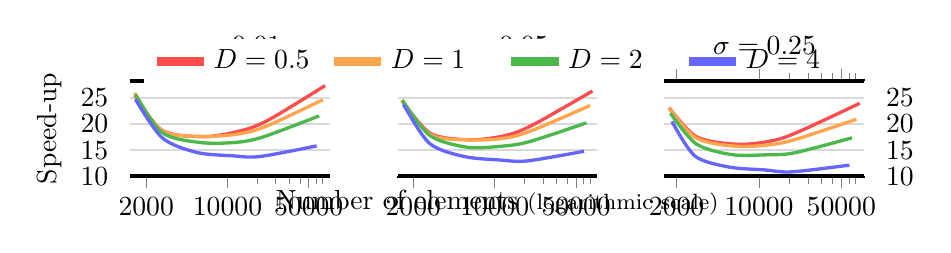
\begin{tikzpicture}
\begin{scope}[shift={(0.0\linewidth,0)}]
\begin{axis}[
 width=0.34\linewidth,height=0.23\linewidth,
 title=\normalsize\mbox{$\sigma=0.01$},
 xmode=log,enlarge x limits=0.025,
 ylabel=Speed-up,
 axis y line*=left,
 ymin=10.0051597471,ymax=28.2408860444,
 tick align=outside,
 x axis line style = ultra thick,y axis line style={white},
 xtick={2000,10000,50000},xticklabels={2000,10000,50000},
 minor xtick={18000,26000,34000,42000,58000,66000}, every y tick/.style={white},ymajorgrids,grid style={gray!30,thick}]
\addplot[very thick,mark=none,smooth,color=red!70] table[] {
	1597.56966667 25.5275251316
	2740.0 18.7841823056
	6219.95666667 17.5804429586
	12841.0846667 18.6768877621
	22453.2753333 20.7637856703
	69114.4313333 27.3725181255
};
\addplot[very thick,mark=none,smooth,color=orange!70] table[] {
	1585.37333333 25.9498783455
	2713.76166667 18.7160847167
	5986.56433333 17.6344837222
	12307.4733333 18.0905621557
	21449.891 19.5640752848
	66056.1383333 24.6605445211
};
\addplot[very thick,mark=none,smooth,color=green!60!black!70] table[] {
	1615.85633333 25.7121504339
	2714.83633333 18.4070182023
	5686.62733333 16.4818805093
	11574.5646667 16.4744938048
	20057.094 17.5046989391
	61394.3783333 21.5595966032
};
\addplot[very thick,mark=none,smooth,color=blue!60!] table[] {
	1614.35233333 24.7571959146
	2738.08866667 17.3827751196
	5399.01866667 14.5755860954
	11013.093 13.9126917286
	19064.4793333 13.7776566906
	58529.946 15.816096244
};
!\end{axis}
\end{scope}
\begin{scope}[shift={(0.28\linewidth,0)}]
\begin{axis}[
 width=0.34\linewidth,height=0.23\linewidth,
 title=\normalsize\mbox{$\sigma=0.05$},
 xmode=log,enlarge x limits=0.025,
 xlabel=Number of elements \footnotesize(logarithmic scale),x label style={at={(axis description cs:0.5,-0.05)},anchor=north},
 yticklabels={},
 legend style={at={(0.55,1.45)},legend style={text width=4em},legend style={draw=none},anchor=north,legend columns=-1},
 axis y line*=left,
 ymin=10.0051597471,ymax=28.2408860444,
 tick align=outside,
 x axis line style = ultra thick,y axis line style={white},
 xtick={2000,10000,50000},xticklabels={2000,10000,50000},
 minor xtick={18000,26000,34000,42000,58000,66000}, every y tick/.style={white},ymajorgrids,grid style={gray!30,thick}]
\addlegendimage{line width=3pt,mark=none,red!70}
\addlegendentry{$D=0.5$}
\addlegendimage{line width=3pt,mark=none,orange!70}
\addlegendentry{$D=1$}
\addlegendimage{line width=3pt,mark=none,green!60!black!70}
\addlegendentry{$D=2$}
\addlegendimage{line width=3pt,mark=none,blue!60!}
\addlegendentry{$D=4$}
\addplot[very thick,mark=none,smooth,color=red!70] table[] {
	1608.38566667 24.4659926471
	2815.783 18.1956562094
	6254.791 16.9864033011
	12939.9666667 17.9005473851
	22515.0153333 20.1360757597
	69028.7106667 26.3398551188
};
\addplot[very thick,mark=none,smooth,color=orange!70] table[] {
	1594.41933333 24.48850046
	2784.365 18.0216951646
	6008.57 16.9497131286
	12318.54 17.3141964086
	21444.6516667 18.8633913532
	65971.1733333 23.5688169248
};
\addplot[very thick,mark=none,smooth,color=green!60!black!70] table[] {
	1604.80333333 24.613037448
	2771.266 17.8250591017
	5749.36966667 15.5649910122
	11597.869 15.7636263321
	20081.009 16.6576481283
	61432.4436667 20.2351410695
};
\addplot[very thick,mark=none,smooth,color=blue!60!] table[] {
	1647.27933333 23.7669642857
	2748.387 16.3149134487
	5426.47433333 13.7889187853
	11030.181 13.1104670821
	19092.137 12.9336935041
	58569.6863333 14.7860408541
};
!\end{axis}
\end{scope}
\begin{scope}[shift={(0.56\linewidth,0)}]
\begin{axis}[
 width=0.34\linewidth,height=0.23\linewidth,
 title=\normalsize\mbox{$\sigma=0.25$},
 xmode=log,enlarge x limits=0.025,
 axis y line*=right,
 ymin=10.0051597471,ymax=28.2408860444,
 tick align=outside,
 x axis line style = ultra thick,y axis line style={white},
 xtick={2000,10000,50000},xticklabels={2000,10000,50000},
 minor xtick={18000,26000,34000,42000,58000,66000}, every y tick/.style={white},ymajorgrids,grid style={gray!30,thick}]
\addplot[very thick,mark=none,smooth,color=red!70] table[] {
	1729.68166667 23.1013043478
	2962.25533333 17.5472851492
	6692.924 16.1123559333
	13605.839 16.9014445626
	23499.072 18.8669761847
	71717.803 23.9846285726
};
\addplot[very thick,mark=none,smooth,color=orange!70] table[] {
	1730.17 22.9615384615
	2922.996 17.3384260082
	6278.947 15.7532892666
	12649.4086667 16.0460118146
	21893.7756667 17.2565072379
	67277.523 20.9260917837
};
\addplot[very thick,mark=none,smooth,color=green!60!black!70] table[] {
	1772.74233333 22.0743664312
	2923.30333333 16.2176802925
	5859.619 14.1387084016
	11707.061 14.1041617743
	20179.976 14.4976095905
	61628.7326667 17.358070408
};
\addplot[very thick,mark=none,smooth,color=blue!60!] table[] {
	1824.84966667 20.5146718147
	2863.199 13.8692624698
	5561.88933333 11.7583403815
	11065.8646667 11.2106103656
	19061.8436667 10.8321768128
	58557.4696667 12.1215546771
};
!\end{axis}
\end{scope}
\end{tikzpicture}
\end{center}
\caption{Speed-up results by mesh remodelling - Eppler 376 airfoil}\centering\sffamily\footnotesize
Average of thirty optimisation scenarios\end{figure}

\pagebreak
\subsubsection{Eppler 545}
\vspace*{\fill} \begin{table}[!hp]
\begin{center}
\begin{tabular}{c|cc?c|c?c?c|c|c||c|c}
\multirow{2}{*}{\textbf{\large $\boldsymbol{\sigma}$}} & \multirow{2}{*}{\textbf{\large $\boldsymbol{I}$}} & \multirow{2}{*}{\textbf{\large $\boldsymbol{G}$}} & \multicolumn{2}{c?}{\textbf{\large Generation}} & \multirow{2}{*}{\textbf{\large $\boldsymbol{D}$}} & \multicolumn{5}{c}{\textbf{{\large Remodelling} }} \\\cline{4-5}\cline{7-11}
 & & & \textbf{\# Tri.} & \textbf{Time} & &\textbf{\# Tri.} & \textbf{Time} & \textbf{Preserv.} & \textbf{+ Tri.} & \textbf{Sp.-up} \\\toprule
\multirow{24}[11]{*}{.01} & \multirow{4}{*}{50} & \multirow{4}{*}{1} & \multirow{4}{*}{1175} & \multirow{4}{*}{1.79 ms} & .5 & 1286 & 0.05 ms & 91.41 \% & 9.46 \% & 32.61 \\\cline{6-11}
 & & & &  & 1 & 1288 & 0.05 ms & 91.42 \% & 9.61 \% & 32.55 \\\cline{6-11}
 & & & &  & 2 & 1299 & 0.05 ms & 91.50 \% & 10.59 \% & 33.19 \\\cline{6-11}
 & & & &  & 4 & 1298 & 0.05 ms & 91.59 \% & 10.47 \% & 34.17 \\\cmidrule[1.5pt]{2-11}
 & \multirow{4}{*}{100} & \multirow{4}{*}{2} & \multirow{4}{*}{1832} & \multirow{4}{*}{3.38 ms} & .5 & 2338 & 0.14 ms & 90.42 \% & 27.63 \% & 24.88 \\\cline{6-11}
 & & & &  & 1 & 2340 & 0.13 ms & 90.46 \% & 27.72 \% & 25.31 \\\cline{6-11}
 & & & &  & 2 & 2327 & 0.13 ms & 90.39 \% & 27.04 \% & 25.33 \\\cline{6-11}
 & & & &  & 4 & 2329 & 0.13 ms & 90.52 \% & 27.16 \% & 25.86 \\\cmidrule[1.5pt]{2-11}
 & \multirow{4}{*}{200} & \multirow{4}{*}{4} & \multirow{4}{*}{4635} & \multirow{4}{*}{9.43 ms} & .5 & 5061 & 0.35 ms & 91.13 \% & 9.19 \% & 26.68 \\\cline{6-11}
 & & & &  & 1 & 5079 & 0.35 ms & 91.16 \% & 9.59 \% & 26.70 \\\cline{6-11}
 & & & &  & 2 & 5118 & 0.37 ms & 91.19 \% & 10.42 \% & 25.70 \\\cline{6-11}
 & & & &  & 4 & 5019 & 0.37 ms & 90.99 \% & 8.30 \% & 25.39 \\\cmidrule[1.5pt]{2-11}
 & \multirow{4}{*}{300} & \multirow{4}{*}{6} & \multirow{4}{*}{9838} & \multirow{4}{*}{20.09 ms} & .5 & 10481 & 0.73 ms & 93.31 \% & 6.54 \% & 27.60 \\\cline{6-11}
 & & & &  & 1 & 10513 & 0.73 ms & 93.33 \% & 6.86 \% & 27.41 \\\cline{6-11}
 & & & &  & 2 & 10530 & 0.78 ms & 93.26 \% & 7.04 \% & 25.86 \\\cline{6-11}
 & & & &  & 4 & 10373 & 0.82 ms & 93.03 \% & 5.45 \% & 24.53 \\\cmidrule[1.5pt]{2-11}
 & \multirow{4}{*}{400} & \multirow{4}{*}{8} & \multirow{4}{*}{17344} & \multirow{4}{*}{36.17 ms} & .5 & 18260 & 1.28 ms & 94.67 \% & 5.28 \% & 28.27 \\\cline{6-11}
 & & & &  & 1 & 18295 & 1.32 ms & 94.65 \% & 5.48 \% & 27.32 \\\cline{6-11}
 & & & &  & 2 & 18304 & 1.40 ms & 94.55 \% & 5.54 \% & 25.76 \\\cline{6-11}
 & & & &  & 4 & 18062 & 1.55 ms & 94.27 \% & 4.14 \% & 23.27 \\\cmidrule[1.5pt]{2-11}
 & \multirow{4}{*}{700} & \multirow{4}{*}{14} & \multirow{4}{*}{53884} & \multirow{4}{*}{155.74 ms} & .5 & 56146 & 3.83 ms & 96.61 \% & 4.20 \% & 40.65 \\\cline{6-11}
 & & & &  & 1 & 56228 & 4.08 ms & 96.56 \% & 4.35 \% & 38.16 \\\cline{6-11}
 & & & &  & 2 & 56051 & 4.59 ms & 96.41 \% & 4.02 \% & 33.91 \\\cline{6-11}
 & & & &  & 4 & 55541 & 5.57 ms & 96.08 \% & 3.07 \% & 27.96\\\bottomrule
\end{tabular}\end{center}
\caption{Full results of mesh remodelling for $\sigma=0.01$ - Eppler 545 airfoil}\centering\sffamily\footnotesize
Average of thirty optimisation scenarios\end{table}
 \vspace*{\fill}
\begin{table}[!hp]
\begin{center}
\begin{tabular}{c|cc?c|c?c?c|c|c||c|c}
\multirow{2}{*}{\textbf{\large $\boldsymbol{\sigma}$}} & \multirow{2}{*}{\textbf{\large $\boldsymbol{I}$}} & \multirow{2}{*}{\textbf{\large $\boldsymbol{G}$}} & \multicolumn{2}{c?}{\textbf{\large Generation}} & \multirow{2}{*}{\textbf{\large $\boldsymbol{D}$}} & \multicolumn{5}{c}{\textbf{{\large Remodelling} }} \\\cline{4-5}\cline{7-11}
 & & & \textbf{\# Tri.} & \textbf{Time} & &\textbf{\# Tri.} & \textbf{Time} & \textbf{Preserv.} & \textbf{+ Tri.} & \textbf{Sp.-up} \\\toprule
\multirow{24}[11]{*}{.05} & \multirow{4}{*}{50} & \multirow{4}{*}{1} & \multirow{4}{*}{1170} & \multirow{4}{*}{1.78 ms} & .5 & 1403 & 0.06 ms & 91.95 \% & 19.90 \% & 30.78 \\\cline{6-11}
 & & & &  & 1 & 1403 & 0.06 ms & 91.94 \% & 19.89 \% & 30.31 \\\cline{6-11}
 & & & &  & 2 & 1401 & 0.06 ms & 91.98 \% & 19.75 \% & 31.16 \\\cline{6-11}
 & & & &  & 4 & 1387 & 0.05 ms & 91.97 \% & 18.52 \% & 32.31 \\\cmidrule[1.5pt]{2-11}
 & \multirow{4}{*}{100} & \multirow{4}{*}{2} & \multirow{4}{*}{1832} & \multirow{4}{*}{3.37 ms} & .5 & 2398 & 0.14 ms & 90.62 \% & 30.87 \% & 24.20 \\\cline{6-11}
 & & & &  & 1 & 2419 & 0.14 ms & 90.71 \% & 32.02 \% & 23.99 \\\cline{6-11}
 & & & &  & 2 & 2444 & 0.14 ms & 90.77 \% & 33.37 \% & 23.74 \\\cline{6-11}
 & & & &  & 4 & 2413 & 0.14 ms & 90.75 \% & 31.66 \% & 23.83 \\\cmidrule[1.5pt]{2-11}
 & \multirow{4}{*}{200} & \multirow{4}{*}{4} & \multirow{4}{*}{4635} & \multirow{4}{*}{9.29 ms} & .5 & 5191 & 0.37 ms & 91.26 \% & 11.98 \% & 24.87 \\\cline{6-11}
 & & & &  & 1 & 5204 & 0.38 ms & 91.30 \% & 12.27 \% & 24.71 \\\cline{6-11}
 & & & &  & 2 & 5219 & 0.39 ms & 91.21 \% & 12.59 \% & 23.80 \\\cline{6-11}
 & & & &  & 4 & 5078 & 0.42 ms & 90.88 \% & 9.55 \% & 22.28 \\\cmidrule[1.5pt]{2-11}
 & \multirow{4}{*}{300} & \multirow{4}{*}{6} & \multirow{4}{*}{9838} & \multirow{4}{*}{19.59 ms} & .5 & 10684 & 0.77 ms & 93.36 \% & 8.60 \% & 25.32 \\\cline{6-11}
 & & & &  & 1 & 10707 & 0.77 ms & 93.35 \% & 8.84 \% & 25.30 \\\cline{6-11}
 & & & &  & 2 & 10668 & 0.83 ms & 93.20 \% & 8.44 \% & 23.58 \\\cline{6-11}
 & & & &  & 4 & 10451 & 0.92 ms & 92.85 \% & 6.23 \% & 21.33 \\\cmidrule[1.5pt]{2-11}
 & \multirow{4}{*}{400} & \multirow{4}{*}{8} & \multirow{4}{*}{17342} & \multirow{4}{*}{35.98 ms} & .5 & 18661 & 1.35 ms & 94.68 \% & 7.61 \% & 26.56 \\\cline{6-11}
 & & & &  & 1 & 18670 & 1.44 ms & 94.63 \% & 7.66 \% & 25.05 \\\cline{6-11}
 & & & &  & 2 & 18483 & 1.54 ms & 94.46 \% & 6.58 \% & 23.31 \\\cline{6-11}
 & & & &  & 4 & 18153 & 1.72 ms & 94.08 \% & 4.68 \% & 20.90 \\\cmidrule[1.5pt]{2-11}
 & \multirow{4}{*}{700} & \multirow{4}{*}{14} & \multirow{4}{*}{53880} & \multirow{4}{*}{155.27 ms} & .5 & 57379 & 4.16 ms & 96.58 \% & 6.49 \% & 37.33 \\\cline{6-11}
 & & & &  & 1 & 57488 & 4.55 ms & 96.49 \% & 6.70 \% & 34.13 \\\cline{6-11}
 & & & &  & 2 & 56548 & 5.19 ms & 96.29 \% & 4.95 \% & 29.94 \\\cline{6-11}
 & & & &  & 4 & 55799 & 6.40 ms & 95.87 \% & 3.56 \% & 24.25\\\bottomrule
\end{tabular}\end{center}
\caption{Full results of mesh remodelling for $\sigma=0.05$ - Eppler 545 airfoil}\centering\sffamily\footnotesize
Average of thirty optimisation scenarios\end{table}

\begin{table}[!hp]
\begin{center}
\begin{tabular}{c|cc?c|c?c?c|c|c||c|c}
\multirow{2}{*}{\textbf{\large $\boldsymbol{\sigma}$}} & \multirow{2}{*}{\textbf{\large $\boldsymbol{I}$}} & \multirow{2}{*}{\textbf{\large $\boldsymbol{G}$}} & \multicolumn{2}{c?}{\textbf{\large Generation}} & \multirow{2}{*}{\textbf{\large $\boldsymbol{D}$}} & \multicolumn{5}{c}{\textbf{{\large Remodelling} }} \\\cline{4-5}\cline{7-11}
 & & & \textbf{\# Tri.} & \textbf{Time} & &\textbf{\# Tri.} & \textbf{Time} & \textbf{Preserv.} & \textbf{+ Tri.} & \textbf{Sp.-up} \\\toprule
\multirow{24}[11]{*}{.25} & \multirow{4}{*}{50} & \multirow{4}{*}{1} & \multirow{4}{*}{1168} & \multirow{4}{*}{1.77 ms} & .5 & 1571 & 0.07 ms & 92.58 \% & 34.53 \% & 26.10 \\\cline{6-11}
 & & & &  & 1 & 1577 & 0.07 ms & 92.63 \% & 35.07 \% & 26.03 \\\cline{6-11}
 & & & &  & 2 & 1631 & 0.07 ms & 92.81 \% & 39.68 \% & 25.06 \\\cline{6-11}
 & & & &  & 4 & 1680 & 0.07 ms & 93.01 \% & 43.92 \% & 23.97 \\\cmidrule[1.5pt]{2-11}
 & \multirow{4}{*}{100} & \multirow{4}{*}{2} & \multirow{4}{*}{1832} & \multirow{4}{*}{3.35 ms} & .5 & 2706 & 0.17 ms & 91.48 \% & 47.69 \% & 19.77 \\\cline{6-11}
 & & & &  & 1 & 2695 & 0.17 ms & 91.37 \% & 47.06 \% & 19.76 \\\cline{6-11}
 & & & &  & 2 & 2694 & 0.18 ms & 91.32 \% & 47.01 \% & 18.79 \\\cline{6-11}
 & & & &  & 4 & 2707 & 0.20 ms & 91.12 \% & 47.75 \% & 16.76 \\\cmidrule[1.5pt]{2-11}
 & \multirow{4}{*}{200} & \multirow{4}{*}{4} & \multirow{4}{*}{4635} & \multirow{4}{*}{9.01 ms} & .5 & 6004 & 0.46 ms & 92.11 \% & 29.53 \% & 19.52 \\\cline{6-11}
 & & & &  & 1 & 5761 & 0.49 ms & 91.69 \% & 24.30 \% & 18.45 \\\cline{6-11}
 & & & &  & 2 & 5526 & 0.53 ms & 91.10 \% & 19.21 \% & 17.07 \\\cline{6-11}
 & & & &  & 4 & 5279 & 0.61 ms & 90.28 \% & 13.90 \% & 14.69 \\\cmidrule[1.5pt]{2-11}
 & \multirow{4}{*}{300} & \multirow{4}{*}{6} & \multirow{4}{*}{9829} & \multirow{4}{*}{19.33 ms} & .5 & 12189 & 0.97 ms & 93.82 \% & 24.01 \% & 19.88 \\\cline{6-11}
 & & & &  & 1 & 11659 & 1.04 ms & 93.42 \% & 18.62 \% & 18.63 \\\cline{6-11}
 & & & &  & 2 & 11109 & 1.15 ms & 92.84 \% & 13.02 \% & 16.85 \\\cline{6-11}
 & & & &  & 4 & 10617 & 1.40 ms & 91.94 \% & 8.01 \% & 13.80 \\\cmidrule[1.5pt]{2-11}
 & \multirow{4}{*}{400} & \multirow{4}{*}{8} & \multirow{4}{*}{17325} & \multirow{4}{*}{35.58 ms} & .5 & 21086 & 1.64 ms & 94.93 \% & 21.71 \% & 21.75 \\\cline{6-11}
 & & & &  & 1 & 20235 & 1.82 ms & 94.58 \% & 16.80 \% & 19.57 \\\cline{6-11}
 & & & &  & 2 & 19145 & 2.14 ms & 93.98 \% & 10.51 \% & 16.61 \\\cline{6-11}
 & & & &  & 4 & 18310 & 2.68 ms & 93.07 \% & 5.68 \% & 13.27 \\\cmidrule[1.5pt]{2-11}
 & \multirow{4}{*}{700} & \multirow{4}{*}{14} & \multirow{4}{*}{53838} & \multirow{4}{*}{153.88 ms} & .5 & 64501 & 5.75 ms & 96.57 \% & 19.81 \% & 26.75 \\\cline{6-11}
 & & & &  & 1 & 62186 & 6.62 ms & 96.26 \% & 15.51 \% & 23.24 \\\cline{6-11}
 & & & &  & 2 & 58572 & 7.93 ms & 95.70 \% & 8.79 \% & 19.41 \\\cline{6-11}
 & & & &  & 4 & 56245 & 10.76 ms & 94.77 \% & 4.47 \% & 14.30\\\bottomrule
\end{tabular}\end{center}
\caption{Full results of mesh remodelling for $\sigma=0.25$ - Eppler 545 airfoil}\centering\sffamily\footnotesize
Average of thirty optimisation scenarios\end{table}
 \newpage
\begin{figure}[!h]
\begin{center}
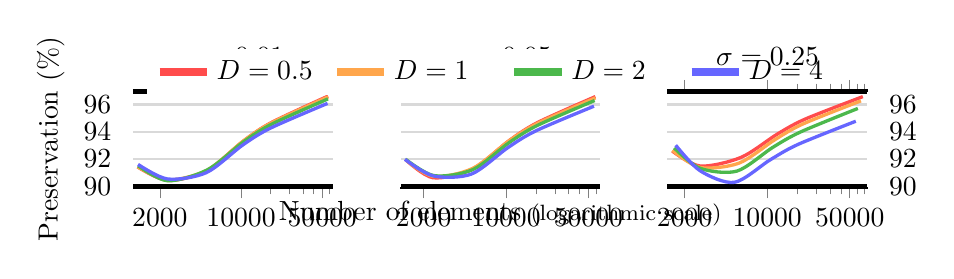
\begin{tikzpicture}
\begin{scope}[shift={(0.0\linewidth,0)}]
\begin{axis}[
 width=0.34\linewidth,height=0.23\linewidth,
 title=\normalsize\mbox{$\sigma=0.01$},
 xmode=log,enlarge x limits=0.025,
 ylabel=Preservation (\%),
 axis y line*=left,
 ymin=89.9630333333,ymax=96.9447983333,
 tick align=outside,
 x axis line style = ultra thick,y axis line style={white},
 xtick={2000,10000,50000},xticklabels={2000,10000,50000},
 minor xtick={18000,26000,34000,42000,58000,66000}, every y tick/.style={white},ymajorgrids,grid style={gray!30,thick}]
\addplot[very thick,mark=none,smooth,color=red!70] table[] {
	1286.178 91.41
	2338.11333333 90.4156666667
	5060.638 91.1263333333
	10480.9623333 93.3123333333
	18259.5173333 94.6713333333
	56146.2446667 96.6123333333
};
\addplot[very thick,mark=none,smooth,color=orange!70] table[] {
	1287.868 91.4186666667
	2339.78233333 90.4593333333
	5079.43933333 91.1566666667
	10512.7686667 93.33
	18294.7776667 94.65
	56228.2326667 96.555
};
\addplot[very thick,mark=none,smooth,color=green!60!black!70] table[] {
	1299.39333333 91.497
	2327.37133333 90.3943333333
	5117.85666667 91.1903333333
	10530.3903333 93.2626666667
	18304.1026667 94.5473333333
	56051.353 96.407
};
\addplot[very thick,mark=none,smooth,color=blue!60!] table[] {
	1297.967 91.5946666667
	2329.49466667 90.524
	5019.41733333 90.9893333333
	10373.4046667 93.0296666667
	18062.391 94.2743333333
	55540.5183333 96.0763333333
};
!\end{axis}
\end{scope}
\begin{scope}[shift={(0.28\linewidth,0)}]
\begin{axis}[
 width=0.34\linewidth,height=0.23\linewidth,
 title=\normalsize\mbox{$\sigma=0.05$},
 xmode=log,enlarge x limits=0.025,
 xlabel=Number of elements \footnotesize(logarithmic scale),x label style={at={(axis description cs:0.5,-0.05)},anchor=north},
 yticklabels={},
 legend style={at={(0.55,1.45)},legend style={text width=4em},legend style={draw=none},anchor=north,legend columns=-1},
 axis y line*=left,
 ymin=89.9630333333,ymax=96.9447983333,
 tick align=outside,
 x axis line style = ultra thick,y axis line style={white},
 xtick={2000,10000,50000},xticklabels={2000,10000,50000},
 minor xtick={18000,26000,34000,42000,58000,66000}, every y tick/.style={white},ymajorgrids,grid style={gray!30,thick}]
\addlegendimage{line width=3pt,mark=none,red!70}
\addlegendentry{$D=0.5$}
\addlegendimage{line width=3pt,mark=none,orange!70}
\addlegendentry{$D=1$}
\addlegendimage{line width=3pt,mark=none,green!60!black!70}
\addlegendentry{$D=2$}
\addlegendimage{line width=3pt,mark=none,blue!60!}
\addlegendentry{$D=4$}
\addplot[very thick,mark=none,smooth,color=red!70] table[] {
	1402.64766667 91.9493333333
	2398.12266667 90.616
	5190.80333333 91.2553333333
	10683.699 93.3583333333
	18660.8343333 94.6833333333
	57378.944 96.5756666667
};
\addplot[very thick,mark=none,smooth,color=orange!70] table[] {
	1402.59766667 91.9443333333
	2419.20233333 90.7136666667
	5204.22733333 91.2983333333
	10707.4293333 93.35
	18670.1523333 94.6266666667
	57488.2726667 96.4856666667
};
\addplot[very thick,mark=none,smooth,color=green!60!black!70] table[] {
	1400.94966667 91.9796666667
	2443.80233333 90.7723333333
	5218.954 91.2083333333
	10668.4646667 93.205
	18483.2026667 94.4606666667
	56547.8526667 96.2876666667
};
\addplot[very thick,mark=none,smooth,color=blue!60!] table[] {
	1386.54 91.9713333333
	2412.582 90.7493333333
	5078.19633333 90.8846666667
	10451.0006667 92.849
	18152.829 94.0823333333
	55798.5793333 95.87
};
!\end{axis}
\end{scope}
\begin{scope}[shift={(0.56\linewidth,0)}]
\begin{axis}[
 width=0.34\linewidth,height=0.23\linewidth,
 title=\normalsize\mbox{$\sigma=0.25$},
 xmode=log,enlarge x limits=0.025,
 axis y line*=right,
 ymin=89.9630333333,ymax=96.9447983333,
 tick align=outside,
 x axis line style = ultra thick,y axis line style={white},
 xtick={2000,10000,50000},xticklabels={2000,10000,50000},
 minor xtick={18000,26000,34000,42000,58000,66000}, every y tick/.style={white},ymajorgrids,grid style={gray!30,thick}]
\addplot[very thick,mark=none,smooth,color=red!70] table[] {
	1570.67133333 92.5796666667
	2706.189 91.476
	6003.85266667 92.1096666667
	12189.182 93.8243333333
	21086.423 94.9326666667
	64500.948 96.5733333333
};
\addplot[very thick,mark=none,smooth,color=orange!70] table[] {
	1576.92233333 92.63
	2694.657 91.373
	5761.26466667 91.687
	11659.3953333 93.42
	20235.336 94.5796666667
	62185.5713333 96.262
};
\addplot[very thick,mark=none,smooth,color=green!60!black!70] table[] {
	1630.739 92.8083333333
	2693.75533333 91.3153333333
	5525.561 91.1013333333
	11109.2813333 92.838
	19145.2023333 93.9766666667
	58572.3666667 95.7046666667
};
\addplot[very thick,mark=none,smooth,color=blue!60!] table[] {
	1680.32233333 93.006
	2707.413 91.1243333333
	5279.23033333 90.2796666667
	10616.6283333 91.937
	18309.9606667 93.0703333333
	56245.1786667 94.7656666667
};
!\end{axis}
\end{scope}
\end{tikzpicture}
\end{center}
\caption{Element preservation results using mesh remodelling - Eppler 545 airfoil}\centering\sffamily\footnotesize
Average of thirty optimisation scenarios\end{figure}

\begin{figure}[!h]
\begin{center}
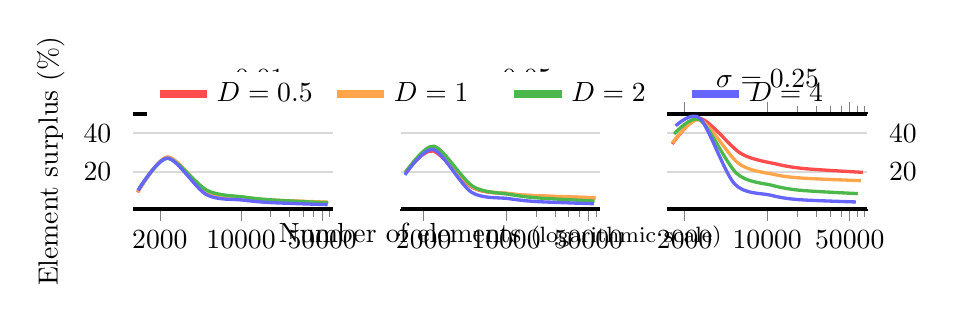
\begin{tikzpicture}
\begin{scope}[shift={(0.0\linewidth,0)}]
\begin{axis}[
 width=0.34\linewidth,height=0.23\linewidth,
 title=\normalsize\mbox{$\sigma=0.01$},
 xmode=log,enlarge x limits=0.025,
 ylabel=Element surplus (\%),
 axis y line*=left,
 ymin=0.839814325036,ymax=50.0990448367,
 tick align=outside,
 x axis line style = ultra thick,y axis line style={white},
 xtick={2000,10000,50000},xticklabels={2000,10000,50000},
 minor xtick={18000,26000,34000,42000,58000,66000}, every y tick/.style={white},ymajorgrids,grid style={gray!30,thick}]
\addplot[very thick,mark=none,smooth,color=red!70] table[] {
	1286.178 9.46363433653
	2338.11333333 27.6288977557
	5060.638 9.18724301441
	10480.9623333 6.54053412093
	18259.5173333 5.27945447888
	56146.2446667 4.19791849298
};
\addplot[very thick,mark=none,smooth,color=orange!70] table[] {
	1287.868 9.60746632714
	2339.78233333 27.720002249
	5079.43933333 9.59289656079
	10512.7686667 6.86385020909
	18294.7776667 5.48275605527
	56228.2326667 4.35007433158
};
\addplot[very thick,mark=none,smooth,color=green!60!black!70] table[] {
	1299.39333333 10.5883607862
	2327.37133333 27.042531988
	5117.85666667 10.4217807273
	10530.3903333 7.04297706014
	18304.1026667 5.5365214914
	56051.353 4.02181563503
};
\addplot[very thick,mark=none,smooth,color=blue!60!] table[] {
	1297.967 10.4669688557
	2329.49466667 27.1584368456
	5019.41733333 8.29787472753
	10373.4046667 5.44719451231
	18062.391 4.14287718289
	55540.5183333 3.07379303305
};
!\end{axis}
\end{scope}
\begin{scope}[shift={(0.28\linewidth,0)}]
\begin{axis}[
 width=0.34\linewidth,height=0.23\linewidth,
 title=\normalsize\mbox{$\sigma=0.05$},
 xmode=log,enlarge x limits=0.025,
 xlabel=Number of elements \footnotesize(logarithmic scale),x label style={at={(axis description cs:0.5,-0.05)},anchor=north},
 yticklabels={},
 legend style={at={(0.55,1.45)},legend style={text width=4em},legend style={draw=none},anchor=north,legend columns=-1},
 axis y line*=left,
 ymin=0.839814325036,ymax=50.0990448367,
 tick align=outside,
 x axis line style = ultra thick,y axis line style={white},
 xtick={2000,10000,50000},xticklabels={2000,10000,50000},
 minor xtick={18000,26000,34000,42000,58000,66000}, every y tick/.style={white},ymajorgrids,grid style={gray!30,thick}]
\addlegendimage{line width=3pt,mark=none,red!70}
\addlegendentry{$D=0.5$}
\addlegendimage{line width=3pt,mark=none,orange!70}
\addlegendentry{$D=1$}
\addlegendimage{line width=3pt,mark=none,green!60!black!70}
\addlegendentry{$D=2$}
\addlegendimage{line width=3pt,mark=none,blue!60!}
\addlegendentry{$D=4$}
\addplot[very thick,mark=none,smooth,color=red!70] table[] {
	1402.64766667 19.8985578356
	2398.12266667 30.872579304
	5190.80333333 11.9820033867
	10683.699 8.59910827089
	18660.8343333 7.60503919662
	57378.944 6.4940432487
};
\addplot[very thick,mark=none,smooth,color=orange!70] table[] {
	1402.59766667 19.8942838272
	2419.20233333 32.0229584676
	5204.22733333 12.2716014155
	10707.4293333 8.84032557203
	18670.1523333 7.6587701144
	57488.2726667 6.69695482121
};
\addplot[very thick,mark=none,smooth,color=green!60!black!70] table[] {
	1400.94966667 19.7534125108
	2443.80233333 33.3654525342
	5218.954 12.5893020739
	10668.4646667 8.4442522594
	18483.2026667 6.58075153012
	56547.8526667 4.95155622775
};
\addplot[very thick,mark=none,smooth,color=blue!60!] table[] {
	1386.54 18.5216717869
	2412.582 31.6616674831
	5078.19633333 9.55271515411
	10451.0006667 6.23374478619
	18152.829 4.67569890942
	55798.5793333 3.56092159416
};
!\end{axis}
\end{scope}
\begin{scope}[shift={(0.56\linewidth,0)}]
\begin{axis}[
 width=0.34\linewidth,height=0.23\linewidth,
 title=\normalsize\mbox{$\sigma=0.25$},
 xmode=log,enlarge x limits=0.025,
 axis y line*=right,
 ymin=0.839814325036,ymax=50.0990448367,
 tick align=outside,
 x axis line style = ultra thick,y axis line style={white},
 xtick={2000,10000,50000},xticklabels={2000,10000,50000},
 minor xtick={18000,26000,34000,42000,58000,66000}, every y tick/.style={white},ymajorgrids,grid style={gray!30,thick}]
\addplot[very thick,mark=none,smooth,color=red!70] table[] {
	1570.67133333 34.5323387715
	2706.189 47.6865690648
	6003.85266667 29.533117732
	12189.182 24.0115914702
	21086.423 21.710381548
	64500.948 19.8058475403
};
\addplot[very thick,mark=none,smooth,color=orange!70] table[] {
	1576.92233333 35.0677541903
	2694.657 47.057225913
	5761.26466667 24.2992817755
	11659.3953333 18.6215917415
	20235.336 16.7979256279
	62185.5713333 15.5052027819
};
\addplot[very thick,mark=none,smooth,color=green!60!black!70] table[] {
	1630.739 39.677300362
	2693.75533333 47.008018686
	5525.561 19.2139753066
	11109.2813333 13.0247836349
	19145.2023333 10.5056974719
	58572.3666667 8.79393634554
};
\addplot[very thick,mark=none,smooth,color=blue!60!] table[] {
	1680.32233333 43.9242498388
	2707.413 47.7533671932
	5279.23033333 13.8993913189
	10616.6283333 8.01257833908
	18309.9606667 5.68470047616
	56245.1786667 4.47135288948
};
!\end{axis}
\end{scope}
\end{tikzpicture}
\end{center}
\caption{Element surplus results on meshes from mesh remodelling - Eppler 545 airfoil}\centering\sffamily\footnotesize
Average of thirty optimisation scenarios\end{figure}

\begin{figure}[!h]
\begin{center}
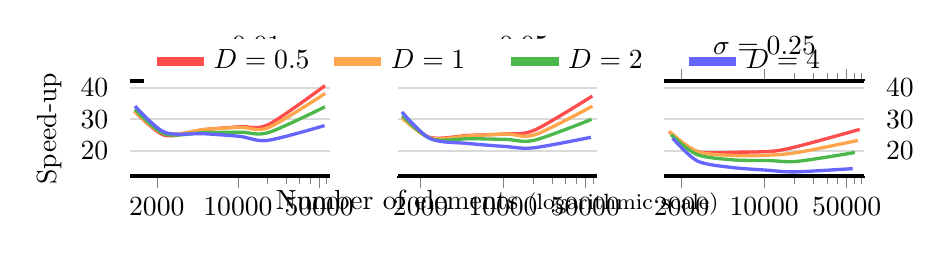
\begin{tikzpicture}
\begin{scope}[shift={(0.0\linewidth,0)}]
\begin{axis}[
 width=0.34\linewidth,height=0.23\linewidth,
 title=\normalsize\mbox{$\sigma=0.01$},
 xmode=log,enlarge x limits=0.025,
 ylabel=Speed-up,
 axis y line*=left,
 ymin=11.9003817799,ymax=42.0848725132,
 tick align=outside,
 x axis line style = ultra thick,y axis line style={white},
 xtick={2000,10000,50000},xticklabels={2000,10000,50000},
 minor xtick={18000,26000,34000,42000,58000,66000}, every y tick/.style={white},ymajorgrids,grid style={gray!30,thick}]
\addplot[very thick,mark=none,smooth,color=red!70] table[] {
	1286.178 32.6086427267
	2338.11333333 24.8843888071
	5060.638 26.6782075472
	10480.9623333 27.6003663004
	18259.5173333 28.2661821781
	56146.2446667 40.6475158116
};
\addplot[very thick,mark=none,smooth,color=orange!70] table[] {
	1287.868 32.5492102066
	2339.78233333 25.3067898153
	5079.43933333 26.7033994334
	10512.7686667 27.4133430352
	18294.7776667 27.3204179255
	56228.2326667 38.1584384826
};
\addplot[very thick,mark=none,smooth,color=green!60!black!70] table[] {
	1299.39333333 33.1945477076
	2327.37133333 25.3257556832
	5117.85666667 25.7034175604
	10530.3903333 25.8620216235
	18304.1026667 25.7630872961
	56051.353 33.9133495921
};
\addplot[very thick,mark=none,smooth,color=blue!60!] table[] {
	1297.967 34.1683673469
	2329.49466667 25.8619897959
	5019.41733333 25.3872879074
	10373.4046667 24.5336589337
	18062.391 23.2723626927
	55540.5183333 27.9554728541
};
!\end{axis}
\end{scope}
\begin{scope}[shift={(0.28\linewidth,0)}]
\begin{axis}[
 width=0.34\linewidth,height=0.23\linewidth,
 title=\normalsize\mbox{$\sigma=0.05$},
 xmode=log,enlarge x limits=0.025,
 xlabel=Number of elements \footnotesize(logarithmic scale),x label style={at={(axis description cs:0.5,-0.05)},anchor=north},
 yticklabels={},
 legend style={at={(0.55,1.45)},legend style={text width=4em},legend style={draw=none},anchor=north,legend columns=-1},
 axis y line*=left,
 ymin=11.9003817799,ymax=42.0848725132,
 tick align=outside,
 x axis line style = ultra thick,y axis line style={white},
 xtick={2000,10000,50000},xticklabels={2000,10000,50000},
 minor xtick={18000,26000,34000,42000,58000,66000}, every y tick/.style={white},ymajorgrids,grid style={gray!30,thick}]
\addlegendimage{line width=3pt,mark=none,red!70}
\addlegendentry{$D=0.5$}
\addlegendimage{line width=3pt,mark=none,orange!70}
\addlegendentry{$D=1$}
\addlegendimage{line width=3pt,mark=none,green!60!black!70}
\addlegendentry{$D=2$}
\addlegendimage{line width=3pt,mark=none,blue!60!}
\addlegendentry{$D=4$}
\addplot[very thick,mark=none,smooth,color=red!70] table[] {
	1402.64766667 30.7782909931
	2398.12266667 24.2023923445
	5190.80333333 24.8666904613
	10683.699 25.3229503253
	18660.8343333 26.5596102266
	57378.944 37.3333119605
};
\addplot[very thick,mark=none,smooth,color=orange!70] table[] {
	1402.59766667 30.3058555998
	2419.20233333 23.990040313
	5204.22733333 24.7057624113
	10707.4293333 25.2978824137
	18670.1523333 25.0523628261
	57488.2726667 34.1300859473
};
\addplot[very thick,mark=none,smooth,color=green!60!black!70] table[] {
	1400.94966667 31.1560490941
	2443.80233333 23.7423140108
	5218.954 23.8026135975
	10668.4646667 23.5768551945
	18483.2026667 23.3137352312
	56547.8526667 29.9408002571
};
\addplot[very thick,mark=none,smooth,color=blue!60!] table[] {
	1386.54 32.3078787879
	2412.582 23.8318021201
	5078.19633333 22.2837837838
	10451.0006667 21.3308292506
	18152.829 20.8983116481
	55798.5793333 24.2490056848
};
!\end{axis}
\end{scope}
\begin{scope}[shift={(0.56\linewidth,0)}]
\begin{axis}[
 width=0.34\linewidth,height=0.23\linewidth,
 title=\normalsize\mbox{$\sigma=0.25$},
 xmode=log,enlarge x limits=0.025,
 axis y line*=right,
 ymin=11.9003817799,ymax=42.0848725132,
 tick align=outside,
 x axis line style = ultra thick,y axis line style={white},
 xtick={2000,10000,50000},xticklabels={2000,10000,50000},
 minor xtick={18000,26000,34000,42000,58000,66000}, every y tick/.style={white},ymajorgrids,grid style={gray!30,thick}]
\addplot[very thick,mark=none,smooth,color=red!70] table[] {
	1570.67133333 26.1032448378
	2706.189 19.7699271797
	6003.85266667 19.523472483
	12189.182 19.8811327871
	21086.423 21.7471070002
	64500.948 26.7545088903
};
\addplot[very thick,mark=none,smooth,color=orange!70] table[] {
	1576.92233333 26.0264705882
	2694.657 19.7582612116
	5761.26466667 18.4457181849
	11659.3953333 18.62686711
	20235.336 19.5680109991
	62185.5713333 23.2406864818
};
\addplot[very thick,mark=none,smooth,color=green!60!black!70] table[] {
	1630.739 25.0561585654
	2693.75533333 18.7934518241
	5525.561 17.0711714556
	11109.2813333 16.8484469884
	19145.2023333 16.6140329032
	58572.3666667 19.4062526273
};
\addplot[very thick,mark=none,smooth,color=blue!60!] table[] {
	1680.32233333 23.9702031603
	2707.413 16.7641855808
	5279.23033333 14.686623927
	10616.6283333 13.7956605524
	18309.9606667 13.2692929243
	56245.1786667 14.2970665296
};
!\end{axis}
\end{scope}
\end{tikzpicture}
\end{center}
\caption{Speed-up results by mesh remodelling - Eppler 545 airfoil}\centering\sffamily\footnotesize
Average of thirty optimisation scenarios\end{figure}

\pagebreak
\subsubsection{Gottingen 702}
\vspace*{\fill} \begin{table}[!hp]
\begin{center}
\begin{tabular}{c|cc?c|c?c?c|c|c||c|c}
\multirow{2}{*}{\textbf{\large $\boldsymbol{\sigma}$}} & \multirow{2}{*}{\textbf{\large $\boldsymbol{I}$}} & \multirow{2}{*}{\textbf{\large $\boldsymbol{G}$}} & \multicolumn{2}{c?}{\textbf{\large Generation}} & \multirow{2}{*}{\textbf{\large $\boldsymbol{D}$}} & \multicolumn{5}{c}{\textbf{{\large Remodelling} }} \\\cline{4-5}\cline{7-11}
 & & & \textbf{\# Tri.} & \textbf{Time} & &\textbf{\# Tri.} & \textbf{Time} & \textbf{Preserv.} & \textbf{+ Tri.} & \textbf{Sp.-up} \\\toprule
\multirow{24}[11]{*}{.01} & \multirow{4}{*}{50} & \multirow{4}{*}{1} & \multirow{4}{*}{1122} & \multirow{4}{*}{1.72 ms} & .5 & 1338 & 0.06 ms & 91.61 \% & 19.24 \% & 30.37 \\\cline{6-11}
 & & & &  & 1 & 1343 & 0.06 ms & 91.64 \% & 19.64 \% & 30.38 \\\cline{6-11}
 & & & &  & 2 & 1342 & 0.06 ms & 91.67 \% & 19.54 \% & 31.04 \\\cline{6-11}
 & & & &  & 4 & 1326 & 0.05 ms & 91.74 \% & 18.14 \% & 32.30 \\\cmidrule[1.5pt]{2-11}
 & \multirow{4}{*}{100} & \multirow{4}{*}{2} & \multirow{4}{*}{1891} & \multirow{4}{*}{3.51 ms} & .5 & 2354 & 0.14 ms & 90.46 \% & 24.52 \% & 24.44 \\\cline{6-11}
 & & & &  & 1 & 2336 & 0.14 ms & 90.40 \% & 23.54 \% & 24.51 \\\cline{6-11}
 & & & &  & 2 & 2364 & 0.14 ms & 90.54 \% & 25.05 \% & 24.64 \\\cline{6-11}
 & & & &  & 4 & 2351 & 0.14 ms & 90.55 \% & 24.35 \% & 24.59 \\\cmidrule[1.5pt]{2-11}
 & \multirow{4}{*}{200} & \multirow{4}{*}{4} & \multirow{4}{*}{4598} & \multirow{4}{*}{9.63 ms} & .5 & 5224 & 0.39 ms & 91.33 \% & 13.61 \% & 24.89 \\\cline{6-11}
 & & & &  & 1 & 5220 & 0.39 ms & 91.31 \% & 13.52 \% & 24.71 \\\cline{6-11}
 & & & &  & 2 & 5178 & 0.41 ms & 91.15 \% & 12.61 \% & 23.72 \\\cline{6-11}
 & & & &  & 4 & 5045 & 0.43 ms & 90.83 \% & 9.72 \% & 22.46 \\\cmidrule[1.5pt]{2-11}
 & \multirow{4}{*}{300} & \multirow{4}{*}{6} & \multirow{4}{*}{9724} & \multirow{4}{*}{20.76 ms} & .5 & 10833 & 0.83 ms & 93.44 \% & 11.41 \% & 24.86 \\\cline{6-11}
 & & & &  & 1 & 10744 & 0.83 ms & 93.37 \% & 10.49 \% & 24.99 \\\cline{6-11}
 & & & &  & 2 & 10623 & 0.89 ms & 93.18 \% & 9.24 \% & 23.37 \\\cline{6-11}
 & & & &  & 4 & 10365 & 0.95 ms & 92.81 \% & 6.59 \% & 21.84 \\\cmidrule[1.5pt]{2-11}
 & \multirow{4}{*}{400} & \multirow{4}{*}{8} & \multirow{4}{*}{17197} & \multirow{4}{*}{36.76 ms} & .5 & 18899 & 1.52 ms & 94.76 \% & 9.90 \% & 24.24 \\\cline{6-11}
 & & & &  & 1 & 18702 & 1.58 ms & 94.66 \% & 8.75 \% & 23.31 \\\cline{6-11}
 & & & &  & 2 & 18427 & 1.70 ms & 94.44 \% & 7.15 \% & 21.61 \\\cline{6-11}
 & & & &  & 4 & 18010 & 1.85 ms & 94.03 \% & 4.73 \% & 19.89 \\\cmidrule[1.5pt]{2-11}
 & \multirow{4}{*}{700} & \multirow{4}{*}{14} & \multirow{4}{*}{53404} & \multirow{4}{*}{157.23 ms} & .5 & 57909 & 4.97 ms & 96.63 \% & 8.43 \% & 31.61 \\\cline{6-11}
 & & & &  & 1 & 57364 & 5.35 ms & 96.51 \% & 7.41 \% & 29.38 \\\cline{6-11}
 & & & &  & 2 & 56478 & 5.99 ms & 96.26 \% & 5.76 \% & 26.23 \\\cline{6-11}
 & & & &  & 4 & 55401 & 7.20 ms & 95.82 \% & 3.74 \% & 21.85\\\bottomrule
\end{tabular}\end{center}
\caption{Full results of mesh remodelling for $\sigma=0.01$ - Gottingen 702 airfoil}\centering\sffamily\footnotesize
Average of thirty optimisation scenarios\end{table}
 \vspace*{\fill}
\begin{table}[!hp]
\begin{center}
\begin{tabular}{c|cc?c|c?c?c|c|c||c|c}
\multirow{2}{*}{\textbf{\large $\boldsymbol{\sigma}$}} & \multirow{2}{*}{\textbf{\large $\boldsymbol{I}$}} & \multirow{2}{*}{\textbf{\large $\boldsymbol{G}$}} & \multicolumn{2}{c?}{\textbf{\large Generation}} & \multirow{2}{*}{\textbf{\large $\boldsymbol{D}$}} & \multicolumn{5}{c}{\textbf{{\large Remodelling} }} \\\cline{4-5}\cline{7-11}
 & & & \textbf{\# Tri.} & \textbf{Time} & &\textbf{\# Tri.} & \textbf{Time} & \textbf{Preserv.} & \textbf{+ Tri.} & \textbf{Sp.-up} \\\toprule
\multirow{24}[11]{*}{.05} & \multirow{4}{*}{50} & \multirow{4}{*}{1} & \multirow{4}{*}{1122} & \multirow{4}{*}{1.72 ms} & .5 & 1390 & 0.06 ms & 91.92 \% & 23.89 \% & 29.21 \\\cline{6-11}
 & & & &  & 1 & 1390 & 0.06 ms & 91.96 \% & 23.90 \% & 29.65 \\\cline{6-11}
 & & & &  & 2 & 1404 & 0.06 ms & 92.09 \% & 25.15 \% & 30.10 \\\cline{6-11}
 & & & &  & 4 & 1367 & 0.06 ms & 91.93 \% & 21.91 \% & 30.80 \\\cmidrule[1.5pt]{2-11}
 & \multirow{4}{*}{100} & \multirow{4}{*}{2} & \multirow{4}{*}{1892} & \multirow{4}{*}{3.51 ms} & .5 & 2433 & 0.15 ms & 90.75 \% & 28.64 \% & 23.93 \\\cline{6-11}
 & & & &  & 1 & 2448 & 0.15 ms & 90.82 \% & 29.43 \% & 24.14 \\\cline{6-11}
 & & & &  & 2 & 2451 & 0.15 ms & 90.82 \% & 29.58 \% & 23.97 \\\cline{6-11}
 & & & &  & 4 & 2382 & 0.15 ms & 90.60 \% & 25.91 \% & 23.40 \\\cmidrule[1.5pt]{2-11}
 & \multirow{4}{*}{200} & \multirow{4}{*}{4} & \multirow{4}{*}{4598} & \multirow{4}{*}{9.59 ms} & .5 & 5326 & 0.40 ms & 91.40 \% & 15.83 \% & 23.79 \\\cline{6-11}
 & & & &  & 1 & 5287 & 0.41 ms & 91.32 \% & 14.98 \% & 23.46 \\\cline{6-11}
 & & & &  & 2 & 5244 & 0.42 ms & 91.16 \% & 14.06 \% & 22.76 \\\cline{6-11}
 & & & &  & 4 & 5067 & 0.45 ms & 90.74 \% & 10.20 \% & 21.22 \\\cmidrule[1.5pt]{2-11}
 & \multirow{4}{*}{300} & \multirow{4}{*}{6} & \multirow{4}{*}{9724} & \multirow{4}{*}{20.47 ms} & .5 & 11021 & 0.85 ms & 93.49 \% & 13.34 \% & 23.95 \\\cline{6-11}
 & & & &  & 1 & 10911 & 0.87 ms & 93.39 \% & 12.21 \% & 23.59 \\\cline{6-11}
 & & & &  & 2 & 10719 & 0.93 ms & 93.14 \% & 10.23 \% & 21.95 \\\cline{6-11}
 & & & &  & 4 & 10410 & 1.01 ms & 92.70 \% & 7.06 \% & 20.35 \\\cmidrule[1.5pt]{2-11}
 & \multirow{4}{*}{400} & \multirow{4}{*}{8} & \multirow{4}{*}{17197} & \multirow{4}{*}{36.71 ms} & .5 & 19167 & 1.57 ms & 94.78 \% & 11.46 \% & 23.36 \\\cline{6-11}
 & & & &  & 1 & 18933 & 1.64 ms & 94.65 \% & 10.10 \% & 22.35 \\\cline{6-11}
 & & & &  & 2 & 18579 & 1.76 ms & 94.38 \% & 8.04 \% & 20.80 \\\cline{6-11}
 & & & &  & 4 & 18073 & 1.98 ms & 93.92 \% & 5.10 \% & 18.50 \\\cmidrule[1.5pt]{2-11}
 & \multirow{4}{*}{700} & \multirow{4}{*}{14} & \multirow{4}{*}{53397} & \multirow{4}{*}{156.93 ms} & .5 & 58808 & 5.18 ms & 96.62 \% & 10.13 \% & 30.29 \\\cline{6-11}
 & & & &  & 1 & 58120 & 5.66 ms & 96.47 \% & 8.84 \% & 27.73 \\\cline{6-11}
 & & & &  & 2 & 56917 & 6.32 ms & 96.20 \% & 6.59 \% & 24.82 \\\cline{6-11}
 & & & &  & 4 & 55583 & 7.72 ms & 95.70 \% & 4.09 \% & 20.33\\\bottomrule
\end{tabular}\end{center}
\caption{Full results of mesh remodelling for $\sigma=0.05$ - Gottingen 702 airfoil}\centering\sffamily\footnotesize
Average of thirty optimisation scenarios\end{table}

\begin{table}[!hp]
\begin{center}
\begin{tabular}{c|cc?c|c?c?c|c|c||c|c}
\multirow{2}{*}{\textbf{\large $\boldsymbol{\sigma}$}} & \multirow{2}{*}{\textbf{\large $\boldsymbol{I}$}} & \multirow{2}{*}{\textbf{\large $\boldsymbol{G}$}} & \multicolumn{2}{c?}{\textbf{\large Generation}} & \multirow{2}{*}{\textbf{\large $\boldsymbol{D}$}} & \multicolumn{5}{c}{\textbf{{\large Remodelling} }} \\\cline{4-5}\cline{7-11}
 & & & \textbf{\# Tri.} & \textbf{Time} & &\textbf{\# Tri.} & \textbf{Time} & \textbf{Preserv.} & \textbf{+ Tri.} & \textbf{Sp.-up} \\\toprule
\multirow{24}[13]{*}{.25} & \multirow{4}{*}{50} & \multirow{4}{*}{1} & \multirow{4}{*}{1121} & \multirow{4}{*}{1.72 ms} & .5 & 1543 & 0.07 ms & 92.55 \% & 37.72 \% & 25.41 \\\cline{6-11}
 & & & &  & 1 & 1541 & 0.07 ms & 92.55 \% & 37.55 \% & 25.34 \\\cline{6-11}
 & & & &  & 2 & 1600 & 0.07 ms & 92.75 \% & 42.79 \% & 25.10 \\\cline{6-11}
 & & & &  & 4 & 1619 & 0.07 ms & 92.83 \% & 44.47 \% & 23.83 \\\cmidrule[1.5pt]{2-11}
 & \multirow{4}{*}{100} & \multirow{4}{*}{2} & \multirow{4}{*}{1884} & \multirow{4}{*}{3.48 ms} & .5 & 2673 & 0.17 ms & 91.39 \% & 41.86 \% & 20.62 \\\cline{6-11}
 & & & &  & 1 & 2655 & 0.17 ms & 91.28 \% & 40.93 \% & 20.22 \\\cline{6-11}
 & & & &  & 2 & 2644 & 0.18 ms & 91.19 \% & 40.36 \% & 19.40 \\\cline{6-11}
 & & & &  & 4 & 2621 & 0.20 ms & 90.88 \% & 39.13 \% & 17.48 \\\cmidrule[1.5pt]{2-11}
 & \multirow{4}{*}{200} & \multirow{4}{*}{4} & \multirow{4}{*}{4593} & \multirow{4}{*}{9.31 ms} & .5 & 5964 & 0.49 ms & 92.06 \% & 29.85 \% & 19.16 \\\cline{6-11}
 & & & &  & 1 & 5720 & 0.49 ms & 91.65 \% & 24.52 \% & 18.84 \\\cline{6-11}
 & & & &  & 2 & 5442 & 0.54 ms & 91.02 \% & 18.46 \% & 17.35 \\\cline{6-11}
 & & & &  & 4 & 5228 & 0.62 ms & 90.21 \% & 13.81 \% & 15.01 \\\cmidrule[1.5pt]{2-11}
 & \multirow{4}{*}{300} & \multirow{4}{*}{6} & \multirow{4}{*}{9715} & \multirow{4}{*}{19.76 ms} & .5 & 12115 & 1.02 ms & 93.81 \% & 24.70 \% & 19.45 \\\cline{6-11}
 & & & &  & 1 & 11573 & 1.09 ms & 93.39 \% & 19.13 \% & 18.06 \\\cline{6-11}
 & & & &  & 2 & 10962 & 1.20 ms & 92.78 \% & 12.84 \% & 16.42 \\\cline{6-11}
 & & & &  & 4 & 10509 & 1.43 ms & 91.89 \% & 8.17 \% & 13.82 \\\cmidrule[1.5pt]{2-11}
 & \multirow{4}{*}{400} & \multirow{4}{*}{8} & \multirow{4}{*}{17179} & \multirow{4}{*}{36.42 ms} & .5 & 20964 & 1.80 ms & 94.92 \% & 22.03 \% & 20.23 \\\cline{6-11}
 & & & &  & 1 & 20060 & 2.01 ms & 94.54 \% & 16.77 \% & 18.09 \\\cline{6-11}
 & & & &  & 2 & 18906 & 2.28 ms & 93.95 \% & 10.05 \% & 16.01 \\\cline{6-11}
 & & & &  & 4 & 18156 & 2.81 ms & 93.04 \% & 5.68 \% & 12.95 \\\cmidrule[1.5pt]{2-11}
 & \multirow{4}{*}{700} & \multirow{4}{*}{14} & \multirow{4}{*}{53353} & \multirow{4}{*}{156.36 ms} & .5 & 64139 & 6.59 ms & 96.58 \% & 20.22 \% & 23.74 \\\cline{6-11}
 & & & &  & 1 & 61691 & 7.51 ms & 96.25 \% & 15.63 \% & 20.83 \\\cline{6-11}
 & & & &  & 2 & 57769 & 8.64 ms & 95.69 \% & 8.28 \% & 18.09 \\\cline{6-11}
 & & & &  & 4 & 55778 & 11.45 ms & 94.75 \% & 4.55 \% & 13.65\\\bottomrule
\end{tabular}\end{center}
\caption{Full results of mesh remodelling for $\sigma=0.25$ - Gottingen 702 airfoil}\centering\sffamily\footnotesize
Average of thirty optimisation scenarios\end{table}
 \newpage
\begin{figure}[!h]
\begin{center}
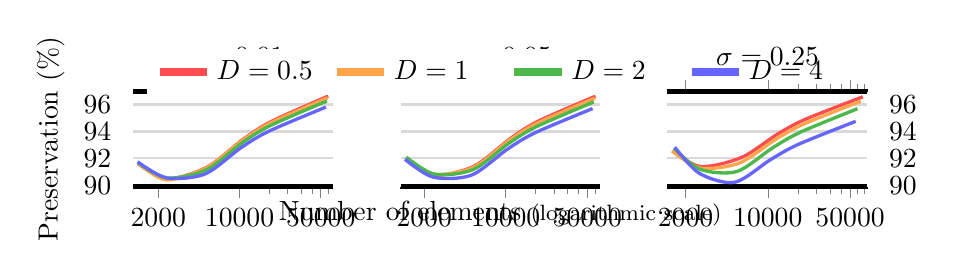
\begin{tikzpicture}
\begin{scope}[shift={(0.0\linewidth,0)}]
\begin{axis}[
 width=0.34\linewidth,height=0.23\linewidth,
 title=\normalsize\mbox{$\sigma=0.01$},
 xmode=log,enlarge x limits=0.025,
 ylabel=Preservation (\%),
 axis y line*=left,
 ymin=89.8934333333,ymax=96.9692783333,
 tick align=outside,
 x axis line style = ultra thick,y axis line style={white},
 xtick={2000,10000,50000},xticklabels={2000,10000,50000},
 minor xtick={18000,26000,34000,42000,58000,66000}, every y tick/.style={white},ymajorgrids,grid style={gray!30,thick}]
\addplot[very thick,mark=none,smooth,color=red!70] table[] {
	1338.169 91.6106666667
	2354.46133333 90.4623333333
	5223.685 91.333
	10833.4676667 93.441
	18899.4443333 94.7553333333
	57908.6903333 96.6323333333
};
\addplot[very thick,mark=none,smooth,color=orange!70] table[] {
	1342.68933333 91.6423333333
	2335.97666667 90.3963333333
	5219.54733333 91.3053333333
	10744.268 93.3693333333
	18701.6783333 94.6576666667
	57363.9423333 96.5106666667
};
\addplot[very thick,mark=none,smooth,color=green!60!black!70] table[] {
	1341.55466667 91.6686666667
	2364.473 90.539
	5177.77766667 91.147
	10622.5566667 93.1793333333
	18426.7493333 94.4386666667
	56478.105 96.264
};
\addplot[very thick,mark=none,smooth,color=blue!60!] table[] {
	1325.89833333 91.7403333333
	2351.403 90.5453333333
	5044.948 90.8346666667
	10364.783 92.8076666667
	18009.931 94.03
	55400.5926667 95.816
};
!\end{axis}
\end{scope}
\begin{scope}[shift={(0.28\linewidth,0)}]
\begin{axis}[
 width=0.34\linewidth,height=0.23\linewidth,
 title=\normalsize\mbox{$\sigma=0.05$},
 xmode=log,enlarge x limits=0.025,
 xlabel=Number of elements \footnotesize(logarithmic scale),x label style={at={(axis description cs:0.5,-0.05)},anchor=north},
 yticklabels={},
 legend style={at={(0.55,1.45)},legend style={text width=4em},legend style={draw=none},anchor=north,legend columns=-1},
 axis y line*=left,
 ymin=89.8934333333,ymax=96.9692783333,
 tick align=outside,
 x axis line style = ultra thick,y axis line style={white},
 xtick={2000,10000,50000},xticklabels={2000,10000,50000},
 minor xtick={18000,26000,34000,42000,58000,66000}, every y tick/.style={white},ymajorgrids,grid style={gray!30,thick}]
\addlegendimage{line width=3pt,mark=none,red!70}
\addlegendentry{$D=0.5$}
\addlegendimage{line width=3pt,mark=none,orange!70}
\addlegendentry{$D=1$}
\addlegendimage{line width=3pt,mark=none,green!60!black!70}
\addlegendentry{$D=2$}
\addlegendimage{line width=3pt,mark=none,blue!60!}
\addlegendentry{$D=4$}
\addplot[very thick,mark=none,smooth,color=red!70] table[] {
	1389.68533333 91.9216666667
	2433.372 90.7496666667
	5325.79166667 91.4043333333
	11020.5346667 93.489
	19167.226 94.7833333333
	58807.7403333 96.6226666667
};
\addplot[very thick,mark=none,smooth,color=orange!70] table[] {
	1389.75633333 91.9636666667
	2448.31266667 90.8216666667
	5286.70233333 91.3246666667
	10910.716 93.391
	18933.2866667 94.65
	58119.686 96.4736666667
};
\addplot[very thick,mark=none,smooth,color=green!60!black!70] table[] {
	1403.82133333 92.09
	2451.14066667 90.8156666667
	5244.49666667 91.161
	10718.5286667 93.1426666667
	18578.6793333 94.3823333333
	56916.5403333 96.201
};
\addplot[very thick,mark=none,smooth,color=blue!60!] table[] {
	1367.433 91.9293333333
	2381.80266667 90.602
	5067.15766667 90.7416666667
	10410.4156667 92.6993333333
	18073.1136667 93.9243333333
	55582.7506667 95.7033333333
};
!\end{axis}
\end{scope}
\begin{scope}[shift={(0.56\linewidth,0)}]
\begin{axis}[
 width=0.34\linewidth,height=0.23\linewidth,
 title=\normalsize\mbox{$\sigma=0.25$},
 xmode=log,enlarge x limits=0.025,
 axis y line*=right,
 ymin=89.8934333333,ymax=96.9692783333,
 tick align=outside,
 x axis line style = ultra thick,y axis line style={white},
 xtick={2000,10000,50000},xticklabels={2000,10000,50000},
 minor xtick={18000,26000,34000,42000,58000,66000}, every y tick/.style={white},ymajorgrids,grid style={gray!30,thick}]
\addplot[very thick,mark=none,smooth,color=red!70] table[] {
	1543.42233333 92.5516666667
	2672.75166667 91.3916666667
	5964.386 92.061
	12114.8056667 93.809
	20963.569 94.9156666667
	64139.478 96.5773333333
};
\addplot[very thick,mark=none,smooth,color=orange!70] table[] {
	1541.49866667 92.5463333333
	2655.24966667 91.2773333333
	5719.593 91.647
	11573.3 93.391
	20059.5583333 94.5443333333
	61690.9613333 96.25
};
\addplot[very thick,mark=none,smooth,color=green!60!black!70] table[] {
	1600.20833333 92.7543333333
	2644.44833333 91.191
	5441.57733333 91.0163333333
	10962.2683333 92.776
	18905.9213333 93.9466666667
	57769.0083333 95.6916666667
};
\addplot[very thick,mark=none,smooth,color=blue!60!] table[] {
	1619.01366667 92.8313333333
	2621.24833333 90.8813333333
	5227.893 90.2143333333
	10509.0943333 91.8943333333
	18155.882 93.0393333333
	55778.1196667 94.7523333333
};
!\end{axis}
\end{scope}
\end{tikzpicture}
\end{center}
\caption{Element preservation results using mesh remodelling - Gottingen 702 airfoil}\centering\sffamily\footnotesize
Average of thirty optimisation scenarios\end{figure}

\begin{figure}[!h]
\begin{center}
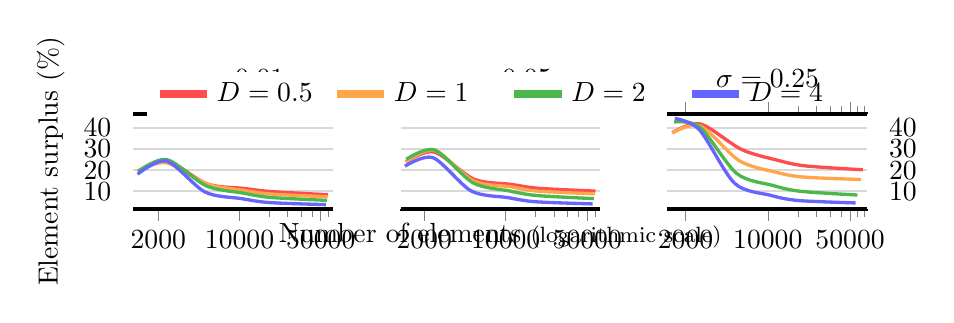
\begin{tikzpicture}
\begin{scope}[shift={(0.0\linewidth,0)}]
\begin{axis}[
 width=0.34\linewidth,height=0.23\linewidth,
 title=\normalsize\mbox{$\sigma=0.01$},
 xmode=log,enlarge x limits=0.025,
 ylabel=Element surplus (\%),
 axis y line*=left,
 ymin=1.70186602962,ymax=46.6055657785,
 tick align=outside,
 x axis line style = ultra thick,y axis line style={white},
 xtick={2000,10000,50000},xticklabels={2000,10000,50000},
 minor xtick={18000,26000,34000,42000,58000,66000}, every y tick/.style={white},ymajorgrids,grid style={gray!30,thick}]
\addplot[very thick,mark=none,smooth,color=red!70] table[] {
	1338.169 19.2370328282
	2354.46133333 24.5164123383
	5223.685 13.6058041046
	10833.4676667 11.40924121
	18899.4443333 9.90127996887
	57908.6903333 8.43475980583
};
\addplot[very thick,mark=none,smooth,color=orange!70] table[] {
	1342.68933333 19.6398153871
	2335.97666667 23.5388450519
	5219.54733333 13.5158172565
	10744.268 10.4919294604
	18701.6783333 8.75126009786
	57363.9423333 7.41471224139
};
\addplot[very thick,mark=none,smooth,color=green!60!black!70] table[] {
	1341.55466667 19.5387113512
	2364.473 25.0458824116
	5177.77766667 12.6074017282
	10622.5566667 9.24027415383
	18426.7493333 7.15253325343
	56478.105 5.75597055833
};
\addplot[very thick,mark=none,smooth,color=blue!60!] table[] {
	1325.89833333 18.1436598057
	2351.403 24.3546714386
	5044.948 9.71859409704
	10364.783 6.58938069193
	18009.931 4.72871234421
	55400.5926667 3.73831499782
};
!\end{axis}
\end{scope}
\begin{scope}[shift={(0.28\linewidth,0)}]
\begin{axis}[
 width=0.34\linewidth,height=0.23\linewidth,
 title=\normalsize\mbox{$\sigma=0.05$},
 xmode=log,enlarge x limits=0.025,
 xlabel=Number of elements \footnotesize(logarithmic scale),x label style={at={(axis description cs:0.5,-0.05)},anchor=north},
 yticklabels={},
 legend style={at={(0.55,1.45)},legend style={text width=4em},legend style={draw=none},anchor=north,legend columns=-1},
 axis y line*=left,
 ymin=1.70186602962,ymax=46.6055657785,
 tick align=outside,
 x axis line style = ultra thick,y axis line style={white},
 xtick={2000,10000,50000},xticklabels={2000,10000,50000},
 minor xtick={18000,26000,34000,42000,58000,66000}, every y tick/.style={white},ymajorgrids,grid style={gray!30,thick}]
\addlegendimage{line width=3pt,mark=none,red!70}
\addlegendentry{$D=0.5$}
\addlegendimage{line width=3pt,mark=none,orange!70}
\addlegendentry{$D=1$}
\addlegendimage{line width=3pt,mark=none,green!60!black!70}
\addlegendentry{$D=2$}
\addlegendimage{line width=3pt,mark=none,blue!60!}
\addlegendentry{$D=4$}
\addplot[very thick,mark=none,smooth,color=red!70] table[] {
	1389.68533333 23.8910724145
	2433.372 28.6410068942
	5325.79166667 15.8262567184
	11020.5346667 13.3356159331
	19167.226 11.4575545868
	58807.7403333 10.1324072375
};
\addplot[very thick,mark=none,smooth,color=orange!70] table[] {
	1389.75633333 23.8974020965
	2448.31266667 29.4308501256
	5286.70233333 14.9761350011
	10910.716 12.2062364062
	18933.2866667 10.0971957109
	58119.686 8.84385100989
};
\addplot[very thick,mark=none,smooth,color=green!60!black!70] table[] {
	1403.82133333 25.1513031716
	2451.14066667 29.5803532708
	5244.49666667 14.0582387167
	10718.5286667 10.229774242
	18578.6793333 8.03515156263
	56916.5403333 6.59065563499
};
\addplot[very thick,mark=none,smooth,color=blue!60!] table[] {
	1367.433 21.9072668909
	2381.80266667 25.9147772158
	5067.15766667 10.2014388594
	10410.4156667 7.06112792056
	18073.1136667 5.09528363967
	55582.7506667 4.09279623917
};
!\end{axis}
\end{scope}
\begin{scope}[shift={(0.56\linewidth,0)}]
\begin{axis}[
 width=0.34\linewidth,height=0.23\linewidth,
 title=\normalsize\mbox{$\sigma=0.25$},
 xmode=log,enlarge x limits=0.025,
 axis y line*=right,
 ymin=1.70186602962,ymax=46.6055657785,
 tick align=outside,
 x axis line style = ultra thick,y axis line style={white},
 xtick={2000,10000,50000},xticklabels={2000,10000,50000},
 minor xtick={18000,26000,34000,42000,58000,66000}, every y tick/.style={white},ymajorgrids,grid style={gray!30,thick}]
\addplot[very thick,mark=none,smooth,color=red!70] table[] {
	1543.42233333 37.7221533982
	2672.75166667 41.860579087
	5964.386 29.8461416995
	12114.8056667 24.7018644369
	20963.569 22.0282568008
	64139.478 20.2176493216
};
\addplot[very thick,mark=none,smooth,color=orange!70] table[] {
	1541.49866667 37.5505014076
	2655.24966667 40.9316323815
	5719.593 24.5169382299
	11573.3 19.1279602328
	20059.5583333 16.7660399625
	61690.9613333 15.6283553771
};
\addplot[very thick,mark=none,smooth,color=green!60!black!70] table[] {
	1600.20833333 42.7892630505
	2644.44833333 40.3583343005
	5441.57733333 18.464469183
	10962.2683333 12.8384009811
	18905.9213333 10.0507563154
	57769.0083333 8.27737615004
};
\addplot[very thick,mark=none,smooth,color=blue!60!] table[] {
	1619.01366667 44.4672943619
	2621.24833333 39.1269571113
	5227.893 13.8125089938
	10509.0943333 8.17372502436
	18155.882 5.68480162618
	55778.1196667 4.5458216842
};
!\end{axis}
\end{scope}
\end{tikzpicture}
\end{center}
\caption{Element surplus results on meshes from mesh remodelling - Gottingen 702 airfoil}\centering\sffamily\footnotesize
Average of thirty optimisation scenarios\end{figure}

\begin{figure}[!h]
\begin{center}
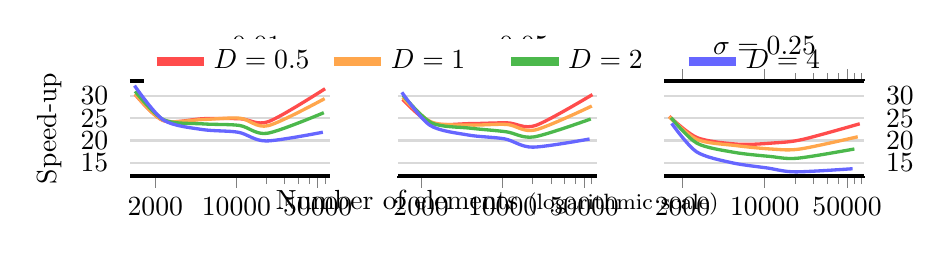
\begin{tikzpicture}
\begin{scope}[shift={(0.0\linewidth,0)}]
\begin{axis}[
 width=0.34\linewidth,height=0.23\linewidth,
 title=\normalsize\mbox{$\sigma=0.01$},
 xmode=log,enlarge x limits=0.025,
 ylabel=Speed-up,
 axis y line*=left,
 ymin=11.9849393289,ymax=33.3198899942,
 tick align=outside,
 x axis line style = ultra thick,y axis line style={white},
 xtick={2000,10000,50000},xticklabels={2000,10000,50000},
 minor xtick={18000,26000,34000,42000,58000,66000}, every y tick/.style={white},ymajorgrids,grid style={gray!30,thick}]
\addplot[very thick,mark=none,smooth,color=red!70] table[] {
	1338.169 30.3668430335
	2354.46133333 24.4443670151
	5223.685 24.8900370275
	10833.4676667 24.8648303393
	18899.4443333 24.2410472862
	57908.6903333 31.6099916234
};
\addplot[very thick,mark=none,smooth,color=orange!70] table[] {
	1342.68933333 30.3847058824
	2335.97666667 24.512695085
	5219.54733333 24.7112934941
	10744.268 24.9905312149
	18701.6783333 23.3148892084
	57363.9423333 29.3826407619
};
\addplot[very thick,mark=none,smooth,color=green!60!black!70] table[] {
	1341.55466667 31.0420673077
	2364.473 24.6447306792
	5177.77766667 23.7177320095
	10622.5566667 23.3685000375
	18426.7493333 21.6109946105
	56478.105 26.2297507702
};
\addplot[very thick,mark=none,smooth,color=blue!60!] table[] {
	1325.89833333 32.3039399625
	2351.403 24.5928955363
	5044.948 22.4625427417
	10364.783 21.8410828249
	18009.931 19.8889129376
	55400.5926667 21.8514224036
};
!\end{axis}
\end{scope}
\begin{scope}[shift={(0.28\linewidth,0)}]
\begin{axis}[
 width=0.34\linewidth,height=0.23\linewidth,
 title=\normalsize\mbox{$\sigma=0.05$},
 xmode=log,enlarge x limits=0.025,
 xlabel=Number of elements \footnotesize(logarithmic scale),x label style={at={(axis description cs:0.5,-0.05)},anchor=north},
 yticklabels={},
 legend style={at={(0.55,1.45)},legend style={text width=4em},legend style={draw=none},anchor=north,legend columns=-1},
 axis y line*=left,
 ymin=11.9849393289,ymax=33.3198899942,
 tick align=outside,
 x axis line style = ultra thick,y axis line style={white},
 xtick={2000,10000,50000},xticklabels={2000,10000,50000},
 minor xtick={18000,26000,34000,42000,58000,66000}, every y tick/.style={white},ymajorgrids,grid style={gray!30,thick}]
\addlegendimage{line width=3pt,mark=none,red!70}
\addlegendentry{$D=0.5$}
\addlegendimage{line width=3pt,mark=none,orange!70}
\addlegendentry{$D=1$}
\addlegendimage{line width=3pt,mark=none,green!60!black!70}
\addlegendentry{$D=2$}
\addlegendimage{line width=3pt,mark=none,blue!60!}
\addlegendentry{$D=4$}
\addplot[very thick,mark=none,smooth,color=red!70] table[] {
	1389.68533333 29.2139219015
	2433.372 23.9292699568
	5325.79166667 23.7874452072
	11020.5346667 23.9501150591
	19167.226 23.3643190496
	58807.7403333 30.2942660241
};
\addplot[very thick,mark=none,smooth,color=orange!70] table[] {
	1389.75633333 29.6502010339
	2448.31266667 24.1378756596
	5286.70233333 23.4557168488
	10910.716 23.5876387662
	18933.2866667 22.3460882974
	58119.686 27.7335764273
};
\addplot[very thick,mark=none,smooth,color=green!60!black!70] table[] {
	1403.82133333 30.0997084548
	2451.14066667 23.9674259681
	5244.49666667 22.7632766126
	10718.5286667 21.9502055407
	18578.6793333 20.8010349582
	56916.5403333 24.8204396879
};
\addplot[very thick,mark=none,smooth,color=blue!60!] table[] {
	1367.433 30.8001193317
	2381.80266667 23.4023576512
	5067.15766667 21.2214269903
	10410.4156667 20.3532316871
	18073.1136667 18.4980769554
	55582.7506667 20.3268440323
};
!\end{axis}
\end{scope}
\begin{scope}[shift={(0.56\linewidth,0)}]
\begin{axis}[
 width=0.34\linewidth,height=0.23\linewidth,
 title=\normalsize\mbox{$\sigma=0.25$},
 xmode=log,enlarge x limits=0.025,
 axis y line*=right,
 ymin=11.9849393289,ymax=33.3198899942,
 tick align=outside,
 x axis line style = ultra thick,y axis line style={white},
 xtick={2000,10000,50000},xticklabels={2000,10000,50000},
 minor xtick={18000,26000,34000,42000,58000,66000}, every y tick/.style={white},ymajorgrids,grid style={gray!30,thick}]
\addplot[very thick,mark=none,smooth,color=red!70] table[] {
	1543.42233333 25.4111549852
	2672.75166667 20.6213496448
	5964.386 19.157638508
	12114.8056667 19.4548587181
	20963.569 20.2277473341
	64139.478 23.7393722545
};
\addplot[very thick,mark=none,smooth,color=orange!70] table[] {
	1541.49866667 25.3361220472
	2655.24966667 20.2223297214
	5719.593 18.8411221256
	11573.3 18.0618811127
	20059.5583333 18.0882708385
	61690.9613333 20.8269176124
};
\addplot[very thick,mark=none,smooth,color=green!60!black!70] table[] {
	1600.20833333 25.1014139444
	2644.44833333 19.4038247308
	5441.57733333 17.3515712334
	10962.2683333 16.4244867426
	18905.9213333 16.0088789908
	57769.0083333 18.0872628141
};
\addplot[very thick,mark=none,smooth,color=blue!60!] table[] {
	1619.01366667 23.8347222222
	2621.24833333 17.4822683172
	5227.893 15.0107451781
	10509.0943333 13.8216134297
	18155.882 12.9525107876
	55778.1196667 13.6547966978
};
!\end{axis}
\end{scope}
\end{tikzpicture}
\end{center}
\caption{Speed-up results by mesh remodelling - Gottingen 702 airfoil}\centering\sffamily\footnotesize
Average of thirty optimisation scenarios\end{figure}

\pagebreak

\end{document}